\documentclass[letterpaper]{book}
\PassOptionsToPackage{usenames,dvipsnames,svgnames,table,xcdraw}{xcolor}
\PassOptionsToPackage{dvipsnames,svgnames,table,xcdraw}{enumitems}


\usepackage{tabularray}
\usepackage{xcolor}


%**************************************************************
%References for commands and symbols:
%1. https://en.wikibooks.org/wiki/LaTeX/Mathematics
%2. http://latex.wikia.com/wiki/List_of_LaTeX_symbols
%**************************************************************
\usepackage{scalerel}
\usepackage{setspace}

%\usepackage{url}
\usepackage{amsmath,amssymb}
\let\proof\relax 
\let\endproof\relax
\usepackage[cm]{fullpage}
%\usepackage{epsfig}
\usepackage{float}
\usepackage{alltt}
%\usepackage{psfrag,xr}
\usepackage[T1]{fontenc}
\usepackage{url}
\usepackage[utf8]{inputenc} % for boxes
\usepackage{pdfpages}
\usepackage{enumerate}
%\includepdfset{pagecommand=\thispagestyle{fancy}}
\usepackage{tcolorbox}
\usepackage[linewidth=1pt]{mdframed}

\usepackage{mathdots}
\usepackage{xfrac}
\usepackage{fix-cm} % Fixes warnings about missing fonts; see http://tex.stackexchange.com/questions/32378/xfrac-siunitx-gives-me-a-font-warning


% Font Settings
\usepackage{avant} % Use the Avantgarde font for headings
%\usepackage{mathptmx} % Use the Adobe Times Roman as the default text font together with math symbols from the Sym­bol, Chancery and Com­puter Modern fonts

\usepackage{subcaption}
%\usepackage{subfig}
\usepackage{graphicx} 
\graphicspath{{graphics/}}
%\usepackage[T1]{fontenc}
%\usepackage[usenames,dvipsnames,svgnames,table, xcdraw]{xcolor}
%\usepackage[caption=false,font=footnotesize]{subfig}
%\usepackage[utf8]{inputenc}
%\usepackage{bmpsize}
% \usepackage{caption}
% \captionsetup{size=footnotesize,
%     %justification=centering, %% not needed
%     skip=5pt, position = bottom}
% \let\proof\relax 
% \let\endproof\relax
%\usepackage{amsthm}
%\usepackage{algorithm}
\usepackage{algorithmicx}
%\usepackage{algpseudocode}
\usepackage{mathrsfs}
\usepackage[ruled,vlined]{algorithm2e}
\usepackage{times}
\usepackage{multicol}
%\usepackage[caption=false,font=footnotesize]{subfig}
\usepackage{amsfonts}
\usepackage[utf8]{inputenc}
\usepackage[T1]{fontenc}
\usepackage{textcomp}
\usepackage{balance}
%\usepackage[sort,numbers]{natbib}
\usepackage{multirow}
\usepackage{booktabs}
\usepackage{dblfloatfix} 

\usepackage{bbm}
\usepackage{bbold}
\usepackage{makecell}
\usepackage{hhline} % double-line in a table
% \usepackage[]{hyperref}
\usepackage[colorlinks]{hyperref}
\definecolor{BrickRed}{rgb}{0.7,0.15,0.15}
\hypersetup{
  colorlinks=true,pdfpagemode=UseNone,citecolor=black,linkcolor=black,urlcolor=BrickRed
}

\usepackage{comment}


\usepackage{xparse}
\usepackage{lipsum}
%\usepackage{subcaption}
\usepackage{soul} 
\usepackage{times}
%\usepackage{cite} % to group references
\usepackage[usenames,dvipsnames,svgnames,table,xcdraw]{xcolor}
% \usepackage[sort, numbers]{natbib}
%\usepackage{balance}
\usepackage{enumitem}


\usepackage{bbding}
%\usepackage{tikz}

% \usepackage{hyperref}
% \usepackage{breakurl}[preserveurlmacro]


\usepackage{listings}
\usepackage{xcolor}
\lstset{literate=
  {á}{{\'a}}1 {é}{{\'e}}1 {í}{{\'i}}1 {ó}{{\'o}}1 {ú}{{\'u}}1
  {Á}{{\'A}}1 {É}{{\'E}}1 {Í}{{\'I}}1 {Ó}{{\'O}}1 {Ú}{{\'U}}1
  {à}{{\`a}}1 {è}{{\`e}}1 {ì}{{\`i}}1 {ò}{{\`o}}1 {ù}{{\`u}}1
  {À}{{\`A}}1 {È}{{\'E}}1 {Ì}{{\`I}}1 {Ò}{{\`O}}1 {Ù}{{\`U}}1
  {ä}{{\"a}}1 {ë}{{\"e}}1 {ï}{{\"i}}1 {ö}{{\"o}}1 {ü}{{\"u}}1
  {Ä}{{\"A}}1 {Ë}{{\"E}}1 {Ï}{{\"I}}1 {Ö}{{\"O}}1 {Ü}{{\"U}}1
  {â}{{\^a}}1 {ê}{{\^e}}1 {î}{{\^i}}1 {ô}{{\^o}}1 {û}{{\^u}}1
  {Â}{{\^A}}1 {Ê}{{\^E}}1 {Î}{{\^I}}1 {Ô}{{\^O}}1 {Û}{{\^U}}1
  {Ã}{{\~A}}1 {ã}{{\~a}}1 {Õ}{{\~O}}1 {õ}{{\~o}}1
  {œ}{{\oe}}1 {Œ}{{\OE}}1 {æ}{{\ae}}1 {Æ}{{\AE}}1 {ß}{{\ss}}1
  {ű}{{\H{u}}}1 {Ű}{{\H{U}}}1 {ő}{{\H{o}}}1 {Ő}{{\H{O}}}1
  {ç}{{\c c}}1 {Ç}{{\c C}}1 {ø}{{\o}}1 {å}{{\r a}}1 {Å}{{\r A}}1
  {€}{{\euro}}1 {£}{{\pounds}}1 {«}{{\guillemotleft}}1
  {»}{{\guillemotright}}1 {ñ}{{\~n}}1 {Ñ}{{\~N}}1 {¿}{{?`}}1
}
\definecolor{codegreen}{rgb}{0,0.6,0}
\definecolor{codegray}{rgb}{0.5,0.5,0.5}
\definecolor{codepurple}{rgb}{0.58,0,0.82}
\definecolor{backcolour}{rgb}{0.95,0.95,0.92}

\lstdefinestyle{mystyle}{
    backgroundcolor=\color{backcolour},   
    commentstyle=\color{codegreen},
    keywordstyle=\color{magenta},
    numberstyle=\tiny\color{black},
    stringstyle=\color{black},
    basicstyle=\ttfamily\normal,
    breakatwhitespace=false,         
    breaklines=true,                 
    captionpos=b,                    
    keepspaces=true,                 
    numbers=left,                    
    numbersep=5pt,                  
    showspaces=false,                
    showstringspaces=false,
    showtabs=false,                  
    tabsize=2
}
\lstset{style=mystyle}


\usepackage{mathtools}
\usepackage[english]{babel}
%\usepackage{minted}

\makeatletter
% \usepackage{tikz}
% \usetikzlibrary{calc}
% \newcommand*\circled[1]{\tikz[baseline=(char.base)]{
%     \node[shape=circle, draw, inner sep=1pt, 
%         minimum height={\f@size*1.6},] (char) {\vphantom{WAH1g}#1};}}
\makeatother

\newcommand{\rb}[1]{\raisebox{1.5ex}{#1}}
 \newcommand{\trace}{\mathrm{trace}}



%\def\real{\mathbb{R}}
\newcommand{\real}{\mathbb R}
\newcommand{\nat}{\mathbb N}   
\newcommand{\whole}{\mathbb Z}    
\newcommand{\cp}{\mathbb C}    
\newcommand{\rat}{\mathbb Q} 
\newcommand{\im}{\mathbb i}
\newcommand{\impart}[1]{\mathrm{imag} ( #1 )}
\newcommand{\repart}[1]{\mathrm{real} ( #1 )}
%\newcommand{\angle}[1]{\mathrm{angle} (#1 )}

%\def\real{\mathbb{R}}
\def\reals{\mathbb{R}} %????

\newcommand{\ds}{\displaystyle}
\newcommand{\mf}[2]{\frac{\ds #1}{\ds #2}}
\newcommand{\book}[2]{{Boyd, Page~#1, }{Prob.~#2}}
\newcommand{\Kuttler}[1]{Kuttler 2017, A First Course in Linear Algebra, Page(s)~#1}
\newcommand{\spanof}[1]{\mathrm{span} \{ #1 \}}
\newcommand{\colspanof}[1]{\mathrm{col~span} \{ #1 \}}
\newcommand{\colspan}[1]{\mathrm{col~span} \{ #1 \}}
\newcommand{\nullspace}[0]{\mathrm{null}}
\newcommand{\nullity}[0]{\mathrm{nullity}}
\newcommand{\range}[0]{\mathrm{range}}
\newcommand{\cost}[0]{\mathrm{f}}
\newcommand{\rank}[0]{\mathrm{rank}}

\newcommand{\pardiff}[2][]{\frac{\partial#1}{\partial#2}}
 \newcommand{\ak}[1]{a_{#1}}


%%%%%%%%%%%%%%%%%%%
% Bruce added below
%%%%%%%%%%%%%%%%%%%
\newcommand{\transpose}{\mathsf{T}}
\DeclareDocumentCommand{\zeros}{ O{} }{\textbf{0}_{#1}}
\newcommand\inv[1]{#1\raisebox{1.15ex}{$\scriptscriptstyle-\!1$}}
\newcommand{\Exp}{\mathrm{Exp}}
\newcommand{\Log}{\mathrm{Log}}
\newtheorem{remark}{Remark}
%%%%%%%%%%%%%%%%%%%
% Bruce added above
%%%%%%%%%%%%%%%%%%%



%\newcommand{\dim}[0]{\mathrm{dim}}
 \newcommand{\cov}{\mathrm{cov}}
  \newcommand{\var}{\mathrm{var}}
 \newcommand{\E}{\mathcal{E}}
  \newcommand{\Expectof}[1]{{\cal E} \{ #1 \}}
  \newcommand{\ExpectofGiven}[2]{{\cal E} \{ #1 | #2 \}}
  \newcommand{\Covof}[2]{ \mathrm{cov} \left(#1,#2\right)}
\parindent 0pt

\newcommand{\notimplies}{%
  \mathrel{{\ooalign{\hidewidth$\not\phantom{=}$\hidewidth\cr$\implies$}}}}


\DeclareMathOperator*{\argmin}{arg\,min}
\DeclareMathOperator*{\argmax}{arg\,max}
\DeclareMathOperator*{\tr}{\rm tr}
\DeclareMathOperator*{\diag}{\rm diag}


\newcommand{\hilight}[1]{\colorbox{yellow}{#1}} % to use: \hl{this is some highlighted text}
\newcommand{\red}[1]{{\textcolor{red}{#1}}}
\newcommand{\blue}[1]{{\textcolor{blue}{#1}}}
\newcommand{\jwg}[1]{[{\textbf{\textcolor{red}{JWG: #1}}}]}
\newcommand{\mgj}[1]{[{\textbf{\textcolor{teal}{Maani: #1}}}]}
\newcommand{\maya}[1]{[{\textbf{\textcolor{blue}{Maya: #1}}}]}


\newcommand\RED{\color{red}}
\newcommand\BLUE{\color{blue}}

\definecolor{note}{rgb}{0.3,0.7,0.25}
\definecolor{rephase}{rgb}{0.15,0.7,0.15}
\definecolor{bag}{rgb}{0.6,0.6,0.2}

 \newcommand\x{\times}
\newcommand\bigzero{\makebox(0,0){\text{\huge0}}}
\newcommand*{\bord}{\multicolumn{1}{c|}{}}
\newcommand*{\bordl}{\multicolumn{1}{|c}{}}

\newcommand*{\Qed}{\hfill $\blacksquare$}

\newcommand\doverline[1]{\ThisStyle{%
  \setbox0=\hbox{$\SavedStyle\overline{#1}$}%
  \ht0=\dimexpr\ht0-.15ex\relax% CHANGE .15 TO AFFECT SPACING
  \overline{\copy0}%
}}

\newcommand{\rob}{\textbb{ROB 101}}

% \newcommand*\circled[1]{\tikz[baseline=(char.base)]{
%     \node[shape=circle, draw, inner sep=1pt, 
%         minimum height={\f@size*1.6},] (char) {\vphantom{WAH1g}#1};}}
\makeatother







\usepackage{listings}
%\usepackage{listingsutf8}
\usepackage[utf8]{inputenc}
\usepackage{xcolor}

\definecolor{dkgreen}{rgb}{0,0.6,0}
\definecolor{gray}{rgb}{0.5,0.5,0.5}
\definecolor{mauve}{rgb}{0.58,0,0.82}
\definecolor{backcolour}{rgb}{0.98,0.92,0.97}
\definecolor{codegray}{rgb}{0.5,0.5,0.5}

%%
%% Julia definition (c) 2014 Jubobs
%%
\lstdefinelanguage{Julia}%
  {morekeywords={abstract,break,case,catch,const,continue,do,else,elseif,%
      end,export,false,for,function,immutable,import,importall,if,in,%
      macro,module,otherwise,quote,return,switch,true,try,type,typealias,%
      using,while},%
   sensitive=true,%
   alsoother={$},%
   morecomment=[l]\#,%
   morecomment=[n]{\#=}{=\#},%
   morestring=[s]{"""}{"""},%
   morestring=[m]{"}{"},%
}[keywords,comments,strings]%

\lstdefinestyle{mystyle}{
frame=tb,
  language=Julia,
  aboveskip=3mm,
  belowskip=3mm,
  showstringspaces=false,
  columns=flexible,
  basicstyle=\ttfamily,
  backgroundcolor=\color{backcolour},
  numberstyle=\tiny{\bf \color{black}},
  keywordstyle={\bf \color{blue}},
  commentstyle=\color{dkgreen},
  identifierstyle={\bf \color{black}},
  stringstyle=\color{mauve},
  breakatwhitespace=false,         
  breaklines=true,                 
  captionpos=b,                    
  keepspaces=true,                 
  numbers=left,                    
  numbersep=5pt,                  
  showspaces=false,                
  showstringspaces=false,
  showtabs=false,                  
  tabsize=2
}

\lstset{style=mystyle}

\lstset{literate=
  {á}{{\'a}}1 {é}{{\'e}}1 {í}{{\'i}}1 {ó}{{\'o}}1 {ú}{{\'u}}1
  {Á}{{\'A}}1 {É}{{\'E}}1 {Í}{{\'I}}1 {Ó}{{\'O}}1 {Ú}{{\'U}}1
  {à}{{\`a}}1 {è}{{\`e}}1 {ì}{{\`i}}1 {ò}{{\`o}}1 {ù}{{\`u}}1
  {À}{{\`A}}1 {È}{{\'E}}1 {Ì}{{\`I}}1 {Ò}{{\`O}}1 {Ù}{{\`U}}1
  {ä}{{\"a}}1 {ë}{{\"e}}1 {ï}{{\"i}}1 {ö}{{\"o}}1 {ü}{{\"u}}1
  {Ä}{{\"A}}1 {Ë}{{\"E}}1 {Ï}{{\"I}}1 {Ö}{{\"O}}1 {Ü}{{\"U}}1
  {â}{{\^a}}1 {ê}{{\^e}}1 {î}{{\^i}}1 {ô}{{\^o}}1 {û}{{\^u}}1
  {Â}{{\^A}}1 {Ê}{{\^E}}1 {Î}{{\^I}}1 {Ô}{{\^O}}1 {Û}{{\^U}}1
  {ã}{{\~a}}1 {ẽ}{{\~e}}1 {ĩ}{{\~i}}1 {õ}{{\~o}}1 {ũ}{{\~u}}1
  {Ã}{{\~A}}1 {Ẽ}{{\~E}}1 {Ĩ}{{\~I}}1 {Õ}{{\~O}}1 {Ũ}{{\~U}}1
  {œ}{{\oe}}1 {Œ}{{\OE}}1 {æ}{{\ae}}1 {Æ}{{\AE}}1 {ß}{{\ss}}1
  {ű}{{\H{u}}}1 {Ű}{{\H{U}}}1 {ő}{{\H{o}}}1 {Ő}{{\H{O}}}1
  {ç}{{\c c}}1 {Ç}{{\c C}}1 {ø}{{\o}}1 {å}{{\r a}}1 {Å}{{\r A}}1
  {€}{{\euro}}1 {£}{{\pounds}}1 {«}{{\guillemotleft}}1
  {»}{{\guillemotright}}1 {ñ}{{\~n}}1 {Ñ}{{\~N}}1 {¿}{{?`}}1 {¡}{{!`}}1 
}

    % commentstyle=\itshape\color{purple!40!black},
    % identifierstyle=\color{blue},
    % backgroundcolor=\color{gray!10!white}
%\parindent

\makeatletter
\renewcommand{\frontmatter}{\cleardoublepage\@mainmatterfalse}
\renewcommand{\mainmatter}{\cleardoublepage\@mainmattertrue}
\makeatother

% \title{Notes for Computational Linear Algebra\thanks{Inspired by Prof. Chad Jenkins}}
% \date{}
% \author{Jessy Grizzle\\ Robotics Institute, University of Michigan, Ann Arbor
% \and Content contributed by Maani, Tribhi, Miley, Madhav, Kira, and Michael}

%\doublespacing

\title{Mathematics for Robotics}
\date{}
\author{Jessy Grizzle\\ Robotics Institute, University of Michigan, Ann Arbor}



\begin{document}
%\maketitle
\newtheorem{thm}{Theorem}
\numberwithin{thm}{chapter}
\newtheorem{example}[thm]{Example}
\newtheorem{nonexample}[thm]{Non-Example}
\newtheorem{prop}[thm]{Proposition}
\newtheorem{lem}[thm]{Lemma}
\newtheorem{cor}[thm]{Corollary}
\newtheorem{claim}[thm]{Claim}
\newtheorem{rem}[thm]{Remark}
\newtheorem{definition}[thm]{Definition}
\newtheorem{notation}[thm]{Notation}
\newtheorem{fact}[thm]{Fact}
\newtheorem{notvocab}[thm]{Notation and Vocabulary}
\newtheorem{question}[thm]{Question}
\newtheorem{recall}[thm]{Recall}
\newtheorem{exercise}[thm]{Exercise}
\newtheorem{summary}[thm]{Summary}
\newcounter{keyfacts}
\newtheorem{keyfact}[keyfacts]{Key Fact}

\begingroup
\thispagestyle{empty}

\AddToShipoutPicture*{\put(-38,0)  {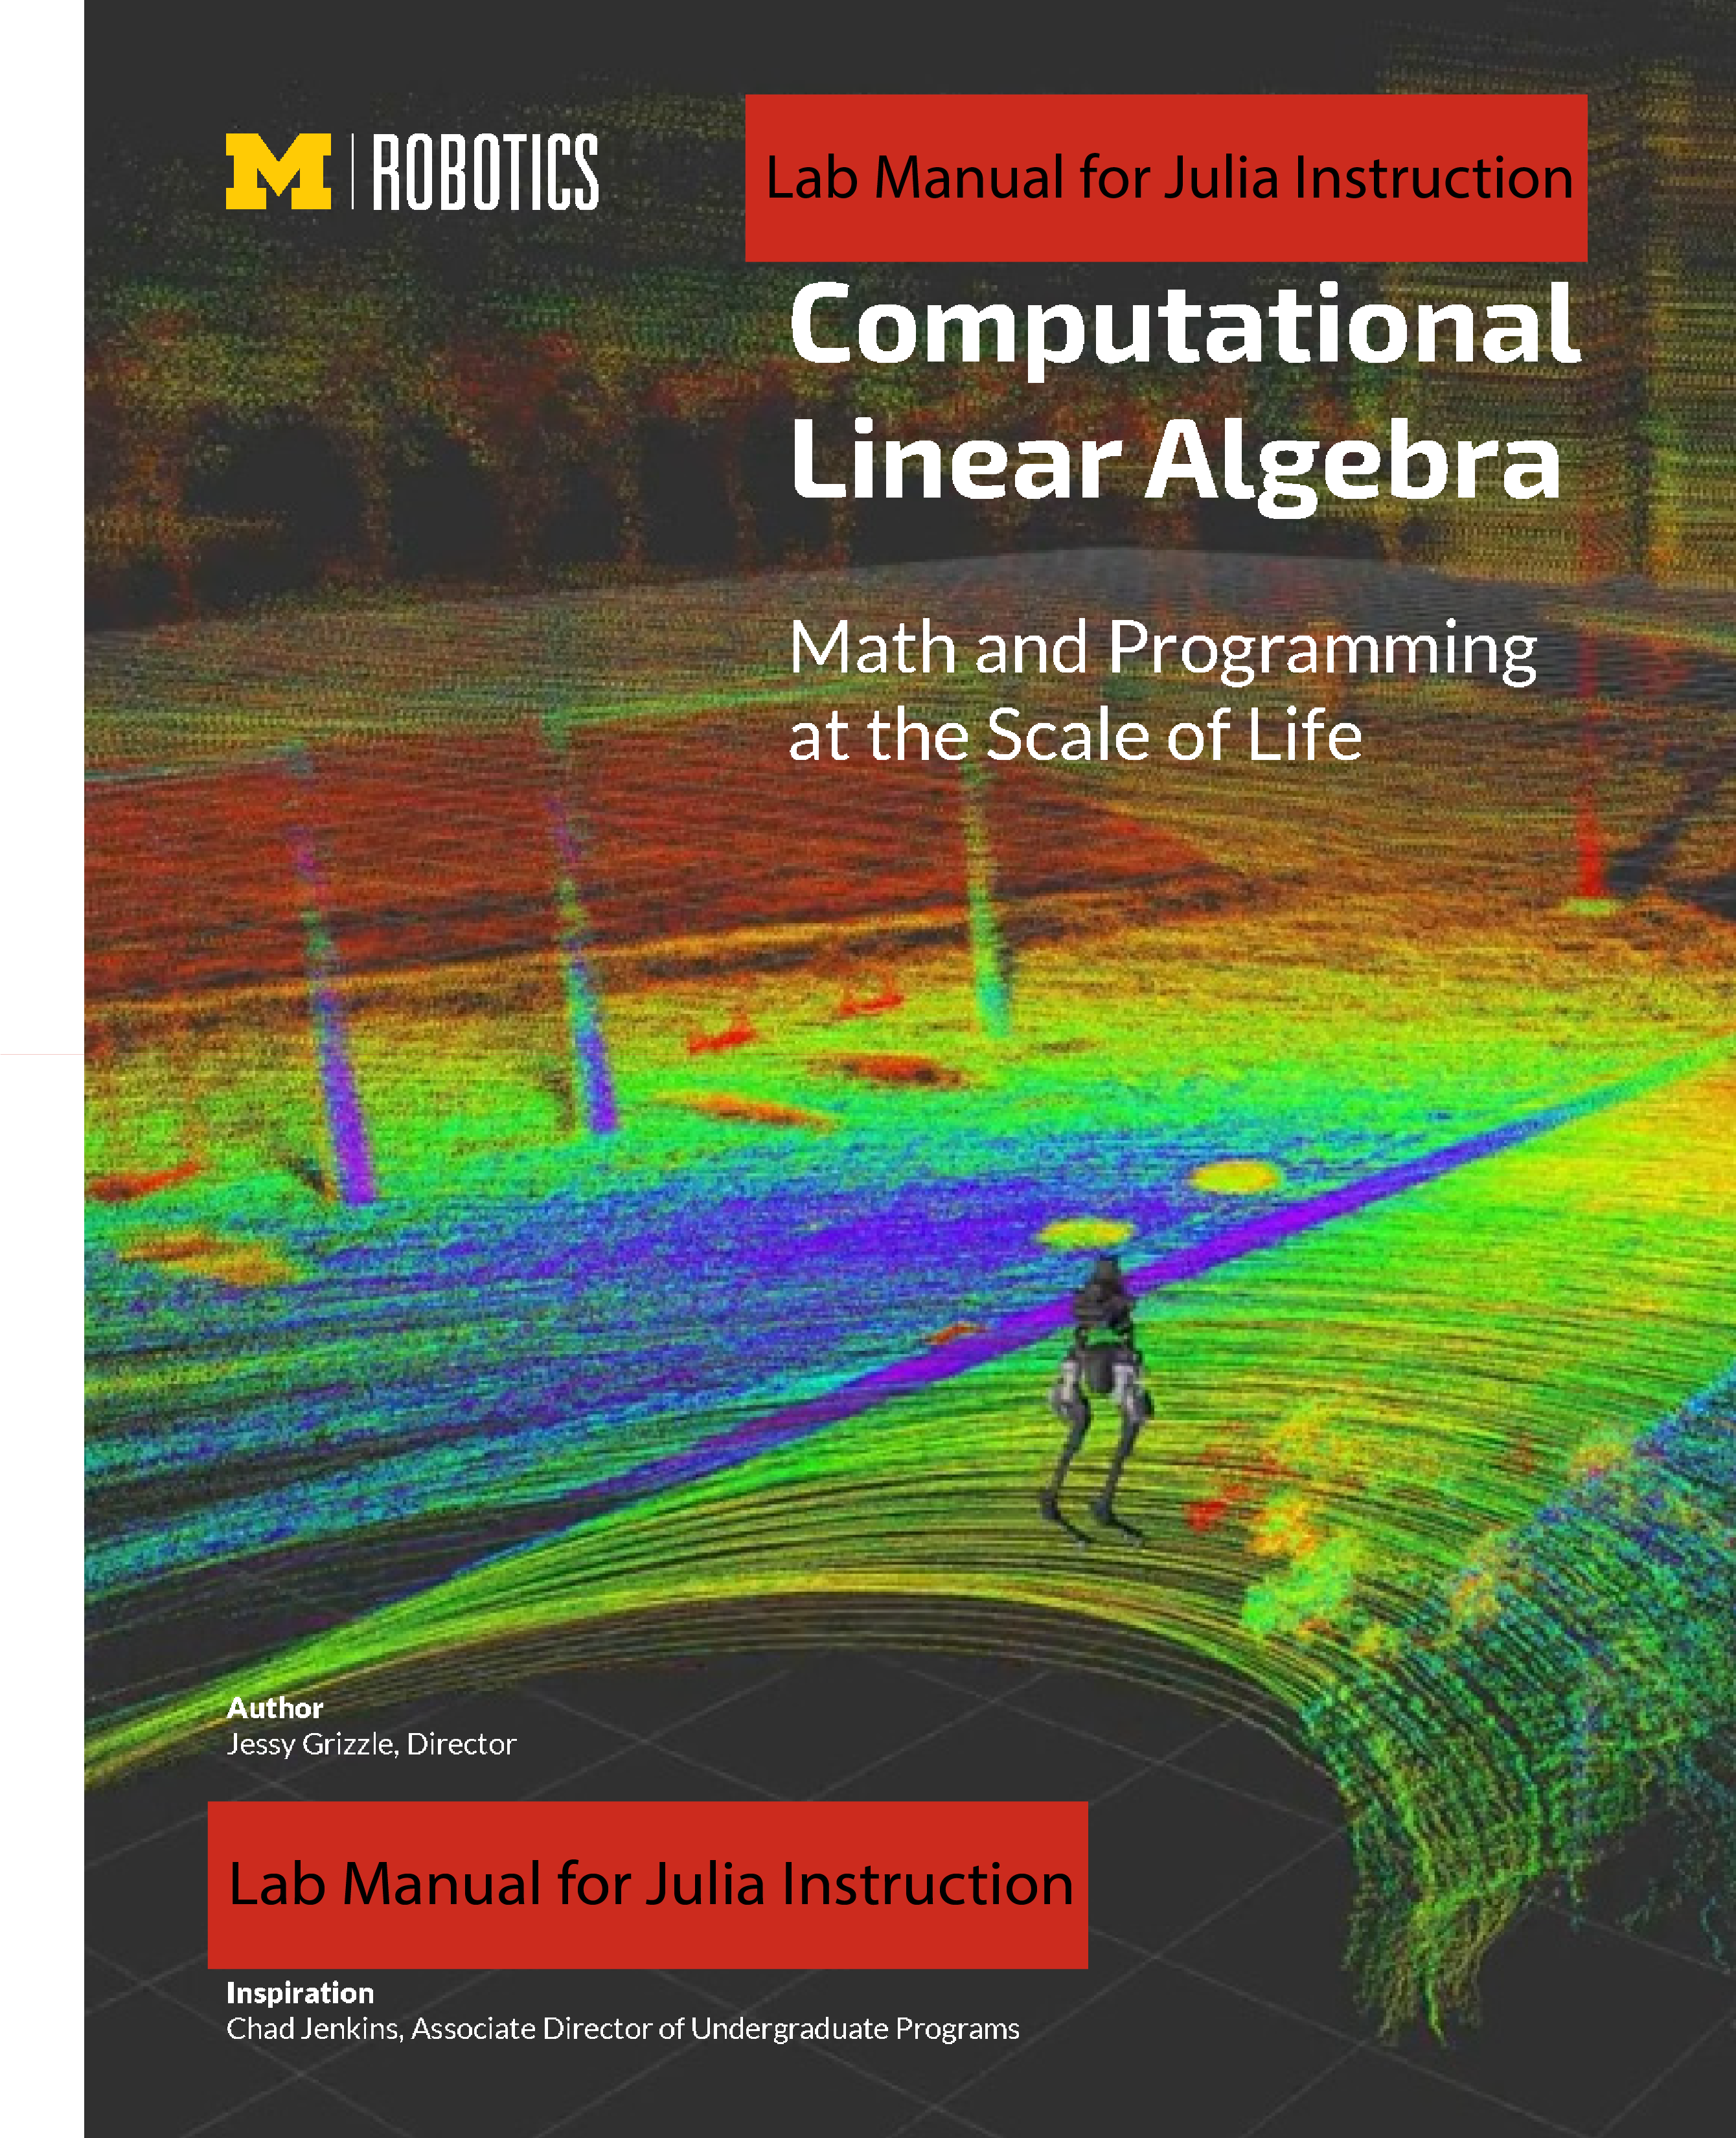
\includegraphics[scale=1.04]{CoverRob101LabManual.png}}} % Image background
\mbox{  }


\endgroup

\clearpage


\begingroup
\thispagestyle{empty}
%\centerline
% \AddToShipoutPicture*{\put(240,50)  {\includegraphics[scale=0.35]{media_users_user_14_project_222374_images_res_cassie_image.png}}} % Image background
\AddToShipoutPicture*{\put(40,450)  {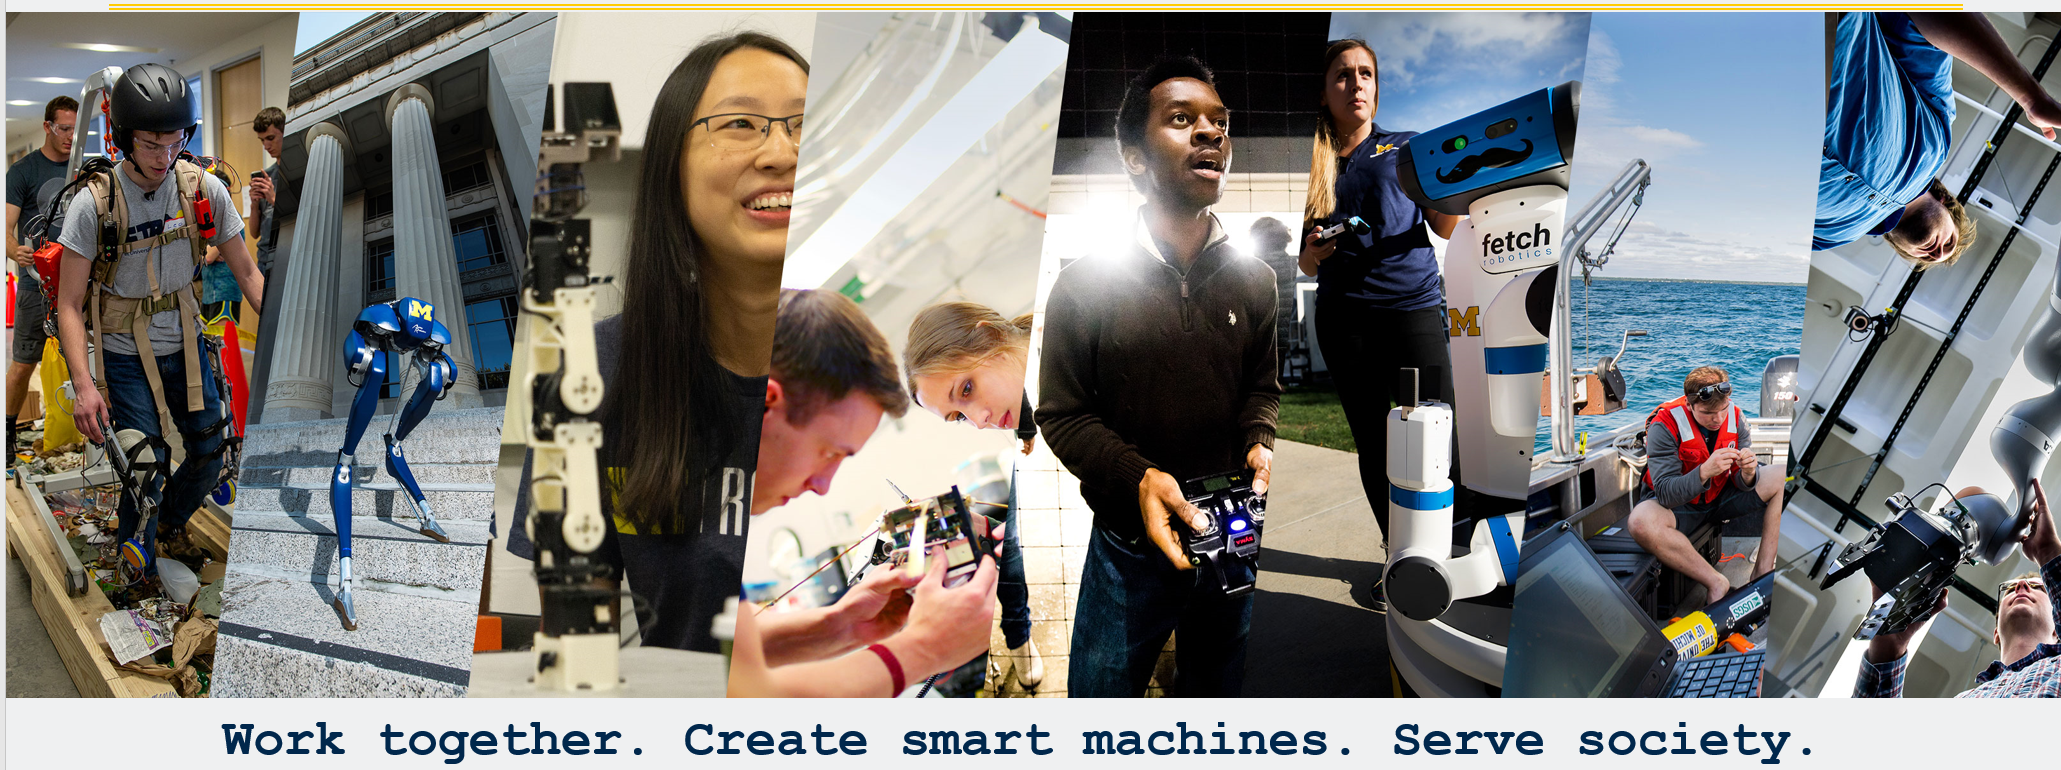
\includegraphics[scale=0.35]{WorkTogether.png}}} % Image background


~\vfill
\thispagestyle{empty}
\noindent Cover design by Dan Newman, Head of Communications, Michigan Robotics

\vspace*{2cm}
\noindent\copyright\space 2022	Jessy Grizzle,  Professor of Robotics, University of Michigan	\\
\noindent \textsc{Jerry W. and Carol L. Levin Professor of Engineering\\
Elmer G. Gilbert Distinguished University Professor}\\

%\noindent \textsc{github.com/LaurethTeX/Clustering}\\ % URL

\noindent This manual is based on the Julia lab exercises that were developed in F-21 by Lu Gan, John Pye, and Jessy Grizzle. Over Su-22, Ms. Yining (Maya) Yuan contributed numerous improvements to the exercises and the editing of the manual.
\\ % License information

\noindent \textit{First release, August 31, 2022. Second Release, January 4, 2023.} % Printing/edition date


\endgroup


\frontmatter
\tableofcontents
\chapter{Preface}
This Julia lab manual goes with the notes for ROB 101, Computational Linear Algebra. Julia is used to transform the theory learned in the course into effective algorithms, or code! The course assumes no prior experience with programming. For those with prior knowledge of MATLAB or C++, Appendices~\ref{App:FromMatlab2Julia} and \ref{App:FromC2Julia} provide hints to help you acquire more quickly some fluency in Julia. A summary of the key Julia commands used in the course is given in Appendix~\ref{App:JuliaCommands}.
\chapter{Philosophy of the Course}
Please see the ROB 101 textbook, which is available online, at no cost \url{https://github.com/michiganrobotics/rob101/tree/main/Fall%202021}. \\

\textbf{Jessy Grizzle}
Ann Arbor, Michigan USA
% \chapter{List of Algorithms and Methods or Things You Need Code to Do Well}
% \input{TexBookletHandouts/ListAlgorithms.tex}
\mainmatter


\setcounter{chapter}{-1}
\chapter{Julia Lab 0: Introduction to Coding in Julia}
\label{chap:Lab0}

\section*{Learning Objectives}

\begin{itemize}
\item What is coding?
\item Getting started with coding at the level of a calculator.
\end{itemize}

\section*{Outcomes} 
\begin{itemize}
\item The Good, The Bad, and the Ugly about Julia
\item What is rounding error
\item Assigning variables
\item Basic arithmetic 
\item Our first dive into an error message
\item A list of built-in functions
\item Rebooting: what to do when all else fails
\item How to learn and keep track of programming skills
\end{itemize}


\newpage

% \begin{figure}[htb!]%
% \centering
% \subfloat[]{%
%     \label{fig:LiDARmap}%
% 	\centering
% 	\setlength{\fboxsep}{0pt}%
% \setlength{\fboxrule}{3pt}%
% \fbox{
% 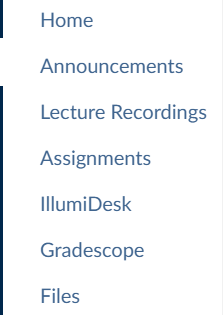
\includegraphics[width=0.25\columnwidth]{Chap00/IllumiDeskLink.png}}%
% }
% \hspace{5pt}%
% \subfloat[]{%
%     \label{fig:Regression}%
% 	\centering
% 		\setlength{\fboxsep}{0pt}%
% \setlength{\fboxrule}{3pt}%
% 	\fbox{
% 
\includegraphics[width=0.7\columnwidth]{Chap00/StartMyServer.png}}%
% }
% \hspace{5pt}%
% \subfloat[]{%
%     \label{fig:Segway}%
% 	\centering
% 			\setlength{\fboxsep}{0pt}%
% \setlength{\fboxrule}{3pt}%
% 	\fbox{
% 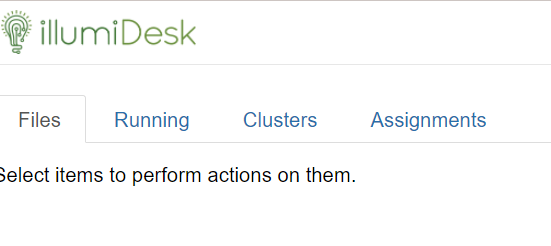
\includegraphics[width=0.35\columnwidth]{Chap00/AssignmentsTab.png}}%
% }
% \hspace{5pt}%
%     \subfloat[]{%
%     \label{fig:GradientDescentIntro}%
% 	\centering
% 			\setlength{\fboxsep}{0pt}%
% \setlength{\fboxrule}{3pt}%
% 	\fbox{
% 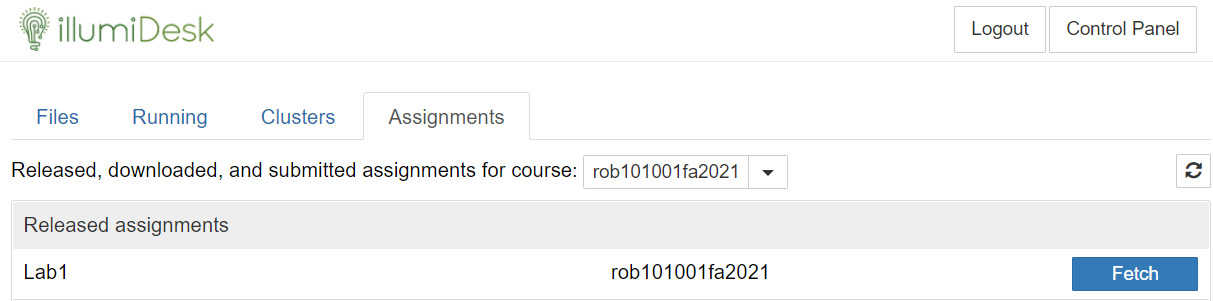
\includegraphics[width=0.6\columnwidth]{Chap00/FetchButton.png}}%
% }
% \hspace{5pt}%
% \subfloat[]{%
%     \label{fig:CameraCalibration}%
% 	\centering
% 			\setlength{\fboxsep}{0pt}%
% \setlength{\fboxrule}{3pt}%
% 	\fbox{
% 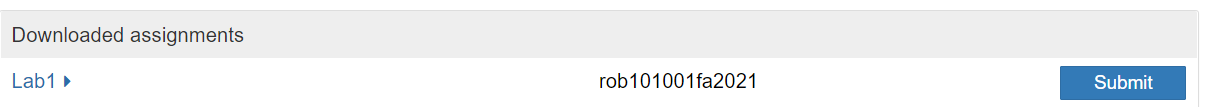
\includegraphics[width=0.9\columnwidth]{Chap00/DownloadedAssignments.png}}%
% }
% \hspace{5pt}%
% \subfloat[]{%
%     \label{fig:ResistorOpAmp}%
% 	\centering
% 			\setlength{\fboxsep}{0pt}%
% \setlength{\fboxrule}{3pt}%
% 	\fbox{
% 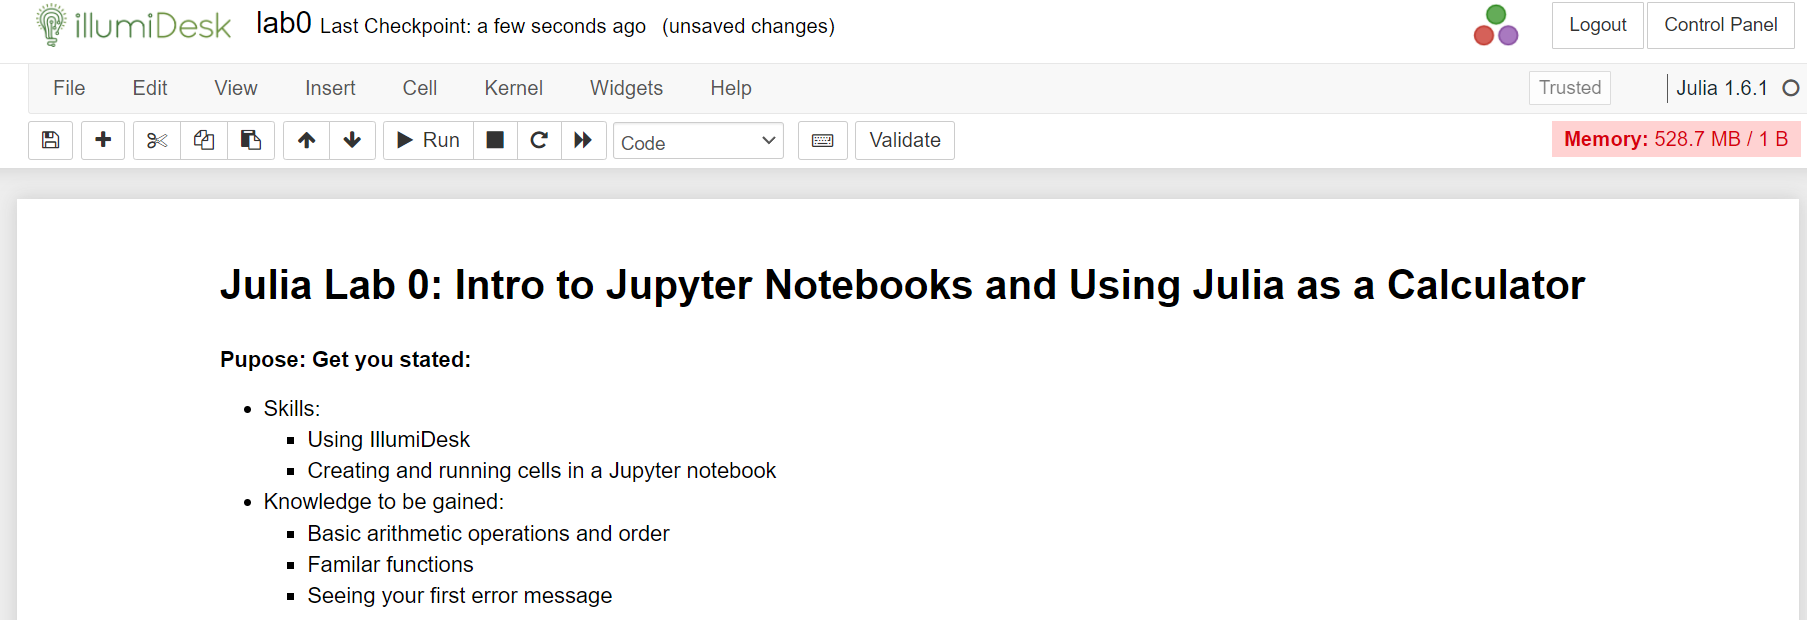
\includegraphics[width=0.8\columnwidth]{Chap00/Lab00Header.png}}%
% }
%     \caption[]{Sequence of steps for accessing your Julia assignments. (a) You start in Canvas, where you click the IllumiDesk link on the left hand side of the page. (b) Once in IllumiDesk, start your sever! (c) Go to the assignments tab. (d) Fetch the assignment. (e) Click on the name of the assignment. \textcolor{red}{\bf For Labs, you never use the submit button. Labs are not graded.}  \textcolor{blue}{\bf Labs are meant to help you with the Julia HW sets, which are graded.} (f) View of a Jupyter notebook.}
%     \label{fig:IllumiDesk}
% \end{figure}


\begin{figure}[htb!]%
\centering
\subfloat[]{%
    \label{fig:LiDARmap}%
	\centering
	\setlength{\fboxsep}{0pt}%
\setlength{\fboxrule}{3pt}%
\fbox{
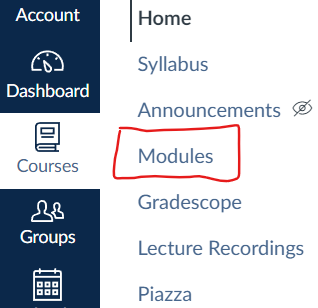
\includegraphics[width=0.25\columnwidth]{graphics/Chap00/VocareumAccessLab00.png}}%
}
\hspace{5pt}%
\subfloat[]{%
    \label{fig:Regression}%
	\centering
		\setlength{\fboxsep}{0pt}%
\setlength{\fboxrule}{3pt}%
	\fbox{
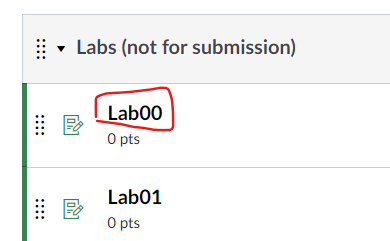
\includegraphics[width=0.25\columnwidth]{graphics/Chap00/VocareumAccessLab00a.png}}%
}
\hspace{5pt}%
\subfloat[]{%
    \label{fig:Segway}%
	\centering
			\setlength{\fboxsep}{0pt}%
\setlength{\fboxrule}{3pt}%
	\fbox{
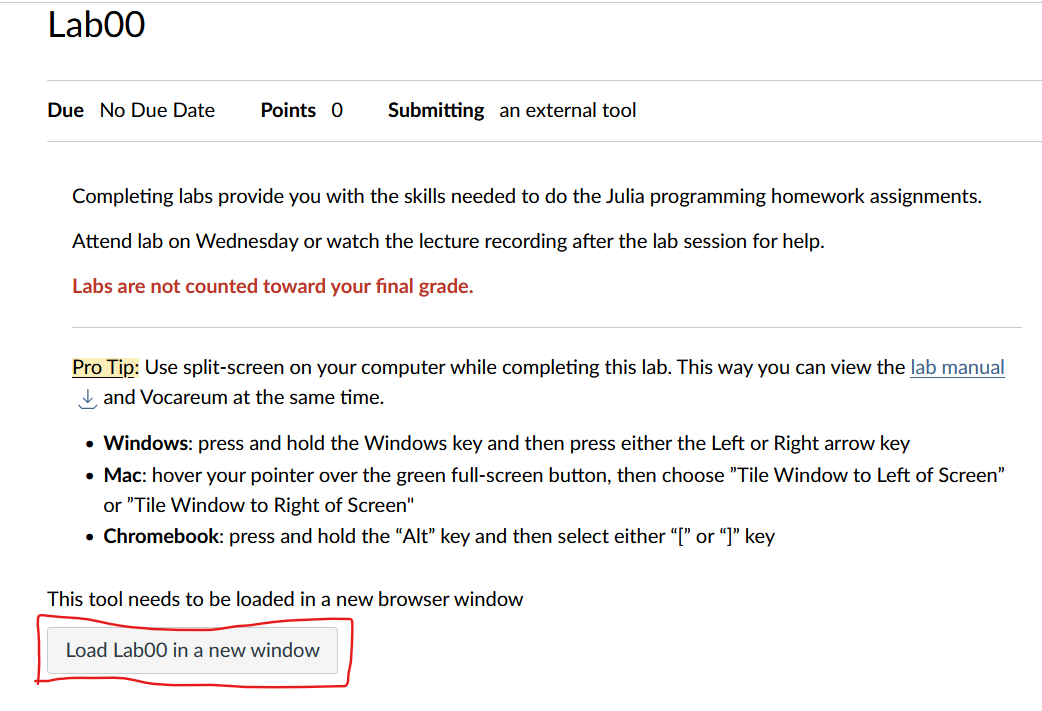
\includegraphics[width=0.4\columnwidth]{graphics/Chap00/VocareumAccessLab00b.png}}%
}
\hspace{5pt}%
    \subfloat[]{%
    \label{fig:GradientDescentIntro}%
	\centering
			\setlength{\fboxsep}{0pt}%
\setlength{\fboxrule}{3pt}%
	\fbox{

\includegraphics[width=0.6\columnwidth]{Chap00/VocareumAccessLab00c.png}}%
}
\hspace{5pt}%
\subfloat[]{%
    \label{fig:CameraCalibration}%
	\centering
			\setlength{\fboxsep}{0pt}%
\setlength{\fboxrule}{3pt}%
	\fbox{
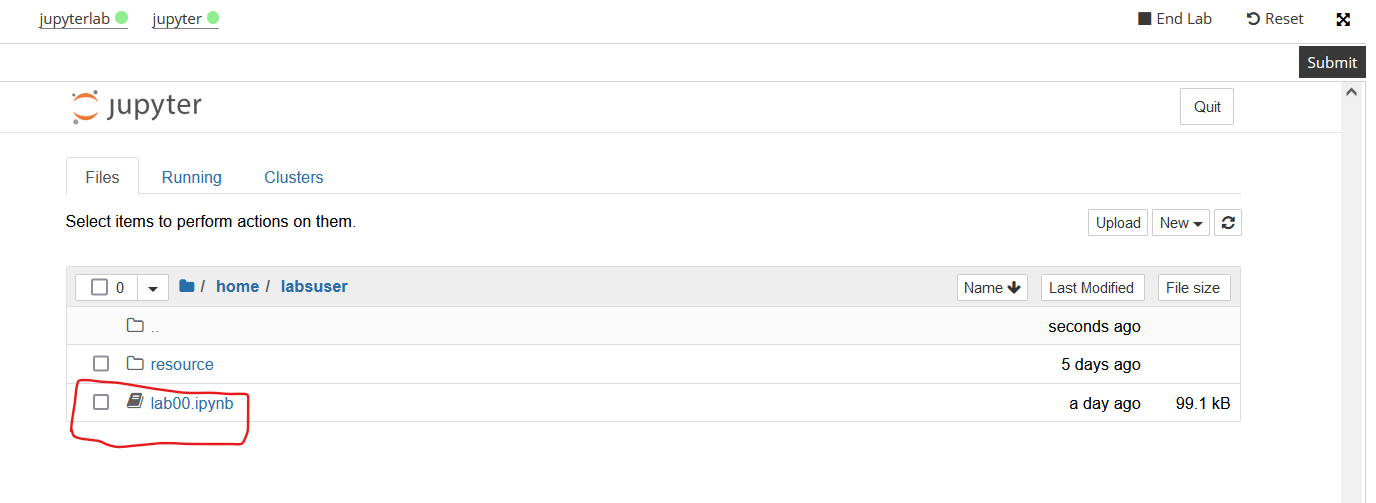
\includegraphics[width=0.65\columnwidth]{Chap00/VocareumAccessLab00d.png}}%
}
\hspace{5pt}%
\subfloat[]{%
    \label{fig:ResistorOpAmp}%
	\centering
			\setlength{\fboxsep}{0pt}%
\setlength{\fboxrule}{3pt}%
	\fbox{
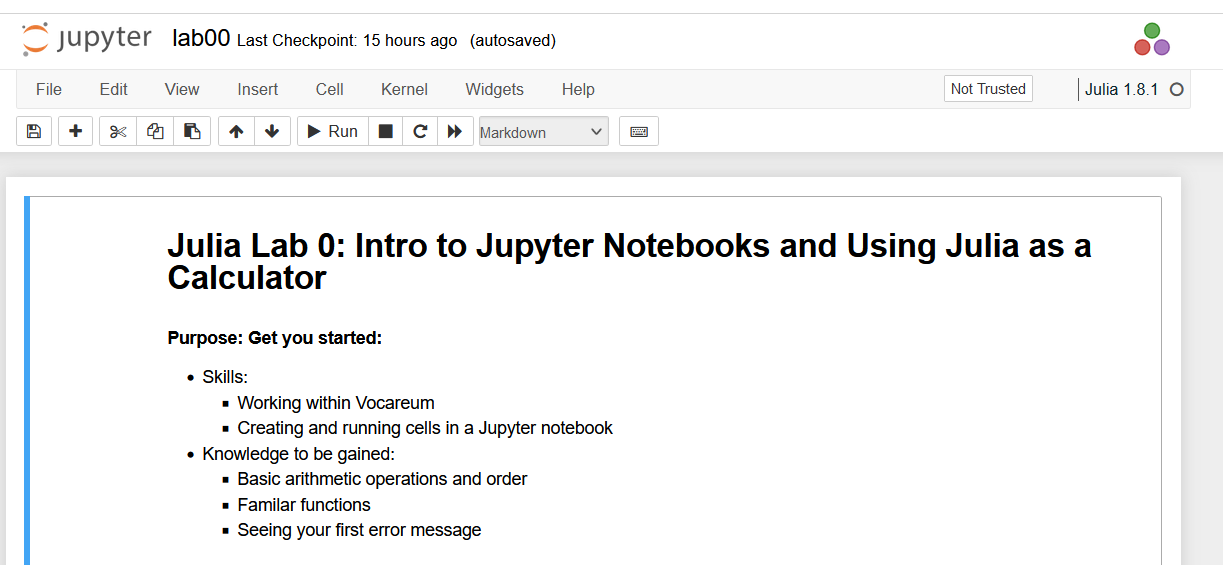
\includegraphics[width=0.7\columnwidth]{Chap00/VocareumAccessLab00e.png}}%
}
    \caption[]{Sequence of steps for accessing your Julia assignments. (a) You start in Canvas, where you click the Modules link on the left hand side of the page. (b) If necessary, scroll down the page until you see the Labs tab or the assignment for the appropriate week. Here we will click on Lab00. (c) Fetch the assignment by clicking on the button that says, Load Lab00 in a new window.  (d) Accept the terms of service for Vocareum. You only have to so this once in the term. (e) Click on the name of the assignment. \textcolor{red}{\bf For Labs, you never use the submit button. Labs are not graded.}  \textcolor{blue}{\bf Labs are meant to help you with the Julia HW sets and the Projects, which are graded.} (f) View of a Jupyter notebook.}
    \label{fig:IllumiDesk}
\end{figure}


\begin{remark}  Hitting the save icon and/or Cntrl-S is completely different than hitting the submit button. You can submit as many times as you want. The last submission is graded. For Julia HW only, if you forget to submit, we automatically grab your latest SAVED copy at 11:59 pm, the day it is due. \textcolor{red}{\bf We do NOT automatically collect your Projects.} Why? Because we allow late submissions with Projects. \textcolor{blue}{\bf If you submit your Project on time and then hit the submit button some other time after the due date, your last submission will be graded and will receive a late penalty.}

\end{remark}

\section{Welcome to ROB 101 and the Julia Programming Language!}

ROB 101 assumes no prior experience with Calculus or programming. These notes are meant for the novice programmer. Learning to program can be fun and frustrating at the same time. Our goal with these notes is to increase the amount of time you have fun and reduce the frustration to the minimum necessary for learning to take place. We all had to touch a hot stove once in our lives! \\ %

If you took programming in High School (HS) or you've already taken ENGR 101 at Michigan, then you have a head start, perhaps. I say perhaps, because Julia is similar to MATLAB, and being a pretty good MATLAB programmer, I expected to pick up Julia in a flash. Wrong! There are just enough maddening differences that I was super frustrated for the first month to six weeks. The same will be true of those of you who know C++. To help you out, in the Appendix, you will find helpful hints to speed your transition into Julia. You can find many sites like this one for additional help \url{https://github.com/brenhinkeller/JuliaAdviceForMatlabProgrammers}. When you find even better sites, please let us know.\\

If you did not take programming in High School, these notes are meant for you! You'll find that learning math and programming at the same time is a much richer and more meaningful experience than learning math alone. My colleague Prof Chad Jenkins coined the phrase, ``Programming = Believing'', and I think he is right. Our goal is to turn into code almost every equation we see in lecture. Things we would never ever dream of doing by hand become ``cake'' in Julia. \\

\textbf{Why are we using Julia?} For several reasons:
\begin{itemize}
    \item Robotics is working alongside Historically Black Colleges and Universities (HBCUs) \url{https://en.wikipedia.org/wiki/Historically_black_colleges_and_universities}, and eventually other Minority Serving Institutions (MSIs), to offer Robotics instruction either remotely or in house. To support remote instruction, we wanted a programming language that we could deliver via a browser. While most students at engineering-intensive universities can download MATLAB to a laptop for free, that is not true at most institutions of higher learning. 
    \item Julia is open source and hence free to everyone! Robotics is a huge supporter of the open-source movement. Even as a Michigan student with free access to MATLAB, when you leave Michigan, there is no guarantee that your company will have MATLAB because it is quite expensive (multiple thousands of dollars per user (seat)). Because Julia is free, cost is not a limiting factor for its adoption. 
    \item Julia is blazingly fast. When you run a block of code for the first time, it is compiled. Thereafter, you essentially have the speed associated with C++.
    \item Julia is modern and forward looking. As someone who was taught FORTRAN back in the day, it feels good to be sharing with you a language that is likely to stand a significant test of time. 
\end{itemize}

\textbf{Why should we have chosen anything but Julia for ROB 101?} The error messages in Julia are horrible. These will be fixed in Julia 2.0. The most current release is Julia 1.8 and thus we'll have to teach you how to suffer through the error messages and find your mistakes. A second reason would be that Julia is \emph{strongly Typed}, which is the proverbial ``blessing'' and a ``curse''. \\


For the super nerds, you must know about the official website for the Julia programming language \url{https://julialang.org/}. It's promotion of Julia is designed for professional programmers. There is a blog that is kind of fun \url{https://julialang.org/blog/2022/02/10years/} where a group of Julia founders and pioneers look back on the language. \\

All of the Julia work for ROB 101 can be completed in the cloud via a browser. \textbf{You do not need to install Julia on your personal computer! You can complete the assignments with as little as an iPad and a keyboard.} Nevertheless, some of you may want to have your own Julia installation; see  Appendix~\ref{App:MyOwnJulia} for how to do that.
\begin{tcolorbox}[sharp corners, colback=red!30, colframe=yellow!80!red, title=\textbf{\large Warning}]
 If you pursue your own installation, \textbf{we cannot provide IT support. We do not have the person-power to do it.} \textcolor{red}{\bf Moreover, you cannot submit HW or Project assignments from your personal Julia installation.} While you can transfer files from our web-based Julia installation to a  personal installation, do the work there, and then copy your work \textbf{cell by cell} back to the web-based environment, you may find that very tedious. \\

 \textbf{Further Warning:} \textcolor{red}{\bf If you change the name of a web-based assignment, it will not be processed by the autograder and you will score a ZERO on your assignment.}
\end{tcolorbox}
You might, however, create your own installation so that you can work on Julia when you are ``off the grid'', for example, or because ``you like the feel of being in control of your computing environment''. Your author uses both: the class site and a personal installation. 



\section{Vocabulary}

\begin{itemize}
    \item \textbf{Programming} is the act of writing instructions for a computer to follow. \textbf{Coding} is similar to programming...if there is a difference, it would be that you do not ``code'' a computer, you ``program'' it, while the action of writing or composing computer instructions can be called either ``coding'' or ``programming''. 
    \item \textbf{Syntax} is the set of formal rules that govern a language, whether a human language such as Spanish or English, or a computer language, such as Julia or C++. Syntax prescribes the allowed symbols in a language, how they can be combined/ordered, and the role of punctuation. Where a pair of square brackets $[~~~ ]$ is used in Julia to ``index'' or ``slice'' an array of numbers, in MATLAB, one uses instead parentheses $( ~~~ )$. These differences can be maddening, just like ``false friends'' between English and French, such as the word ``special'' having a positive connotation in English and ``speciale'' having a negative connotation in French. How can that be? Or French inserting a space before a question mark at the end of a sentence, while in English, we do not. The challenge with learning a computer language is that it is \textbf{unforgiving of syntax errors}. If you are lucky, it ``throws an error flag'' and identifies the line on which the error occurred. If you are unlucky, what you entered was still legal syntax and the computer does something you never intended, without you suspecting that your instruction actually meant something else. 
    \item A list of \textbf{punctuation symbols} in Julia \url{https://docs.julialang.org/en/v1/base/punctuation/}. We will only encounter a few of them in ROB 101.
    \item \textbf{Debugging} computer code is the process of finding and fixing errors in the code. It could be that the code does not run because the errors were ``fatal'' or the code runs but produces flawed output. You can read more here about the etymology of the term debugging \url{https://en.wikipedia.org/wiki/Debugging}. 
    \item \textbf{Variables} store information that can be referenced or changed in a program; see \url{https://en.wikipedia.org/wiki/Variable_(computer_science)}.
    \item A variable's \textbf{Type} determines the values it can hold and the operations that can be performed on the variable. If a variable's type is \texttt{char} then it can hold characters, such as letters of the alphabet, or common symbols such as $@$ or $\&$. If its type is \texttt{char} and you try to assign a real number to it, you will generate an error. In the computer, a variable's type is used to economize on storage space, because in general it takes more zeros and ones (\textbf{bits}) to specify a real number than it does a letter of the alphabet. Hence allocating a ton of space in memory and then putting the letter D in it is wasteful. Types are also used to indicate what operations can be performed on a variable. For example, letters in the alphabet (variables of \texttt{char} type) can be concatenated to form \texttt{strings}, whereas it does not make so much sense to concatenate $3.14159$ with $1.41421$, because what would you do with an object that had two decimal points? Similarly, it makes sense to add two real numbers (type \texttt{Real}), but not so much the addition of two letters A and M. By assigning \texttt{Types} to all variables, Julia helps you to avoid ``stupid mistakes''. We'll also see that Julia can sometimes be so strict with its imposition of \texttt{Types} that it's maddening. More on this later.
    \item \textbf{Jupyter Notebook} (spelling is correct) ``is an open-source web application that allows data scientists to create and share documents that integrate live code, equations, computational output, visualizations, and other multimedia resources, along with explanatory text in a single document\footnote{\url{https://odsc.medium.com/why-you-should-be-using-jupyter-notebooks-ea2e568c59f2}}.'' Jupyter is sort of a contraction built from the programming languages Julia, Python, and R.  Jupyter Notebooks consist of a sequence of cells, where each cell can hold code, text, plots, typeset equations, images, etc.
    \item \textbf{Vocareum} is the company supporting our web access to Julia and Jupyter notebooks; you can learn more at \url{https://www.vocareum.com/}. 
     \item A more extensive \textbf{glossary of coding terminology} is available here \url{https://code.org/curriculum/docs/k-5/glossary}. 
\end{itemize}

\section{Accessing and Submitting Julia Assignments}
\label{sec:Vocareum}

\textbf{Accessing Labs, HWs, and Projects} All of the Jupyter notebooks used in the course are accessed via the ROB 101 Canvas page; hence you need to be a member of the course's Canvas site to reach it. Once you login to Canvas, you want to 
\begin{itemize}
    \item Click on the Modules link in the left hand panel.
    \item Scroll down until you see what you are after: a Lab, a Julia HW, or a Project. They are mostly listed by the week that an assignment becomes available to you, though Labs can be accessed at any time.
    \item Click on the appropriate link.
    % \item Hit the tan box that says, \boxed{\text{\rm Load XXXX in a new window}}.
    \item Hit the tan box that says, \colorbox{Tan}{\makebox[4.23cm][l]{{\rm Load XXXX in a new window}}}.
    \item Click on the appropriate link.
    \item You should now be in a Jupyter notebook; see Fig.~\ref{fig:IllumiDesk}.
\end{itemize}

\textbf{Julia HW Submission:} While Labs are not submitted, you should submit your Julia HW and your Projects. You do that by hitting the BLACK submit button in the Upper Right corner. You can see all of your submissions by hitting the \textcolor{blue}{Submission >} link in the Upper Left corner. After you hit the link, the arrow will change directions \textcolor{blue}{Submission <}. \\



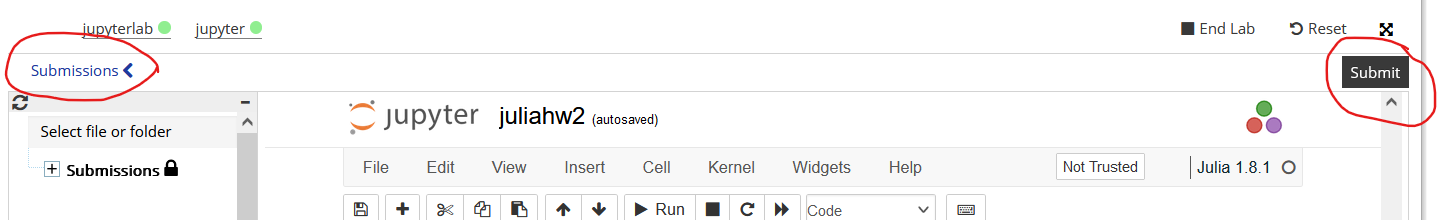
\includegraphics[width=0.9\columnwidth]{graphics/Chap00/Submit.png}%


\section{Learning and Keeping Track of Programming Skills}
\label{sec:GoogleDoc4Commands}

%\vspace*{.2cm}

While we have summarized the most frequently used commands in Appendix~\ref{App:JuliaCommands}, you will learn more quickly if you create your own record of frequently used commands and encountered problems. It is suggested that you make a copy of the following Google Doc \url{https://docs.google.com/document/d/1NnB0dFUKbLAOJ8CIB9YpXj71XhAPFwmTAYOFDDDHR_w/edit?usp=sharing} and add commands to it as you learn them in the course. You must make your own personal copy before you can edit the file. Once you copy the file, you can rename it and add content.\\

Can a group of you share a Google Doc filled with Julia tips and tricks? Sure. It's OK, but you'll probably learn more if you make your own ``cheat sheet''.


\vspace*{.2cm}
\setlength{\fboxrule}{3pt}%
	\centerline{ \fbox{ 
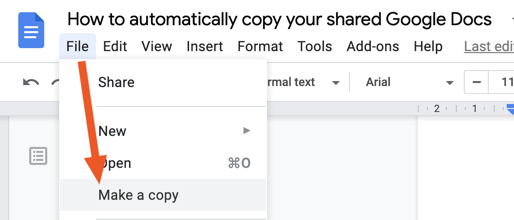
\includegraphics[width=0.5\columnwidth]{Chap00/WildRobotTeacherGuide.png}}%
}

\section{LAB 0: Julia as a Calculator}

This lab gets you started with Julia. You should follow the steps in Chapter~\ref{sec:Vocareum} and open the lab00 Julia notebook, or in your own installation of Julia, open a Julia notebook and try the various basic commands introduced here.\\

\setlength{\fboxrule}{3pt}%
	\centerline{ \fbox{ 
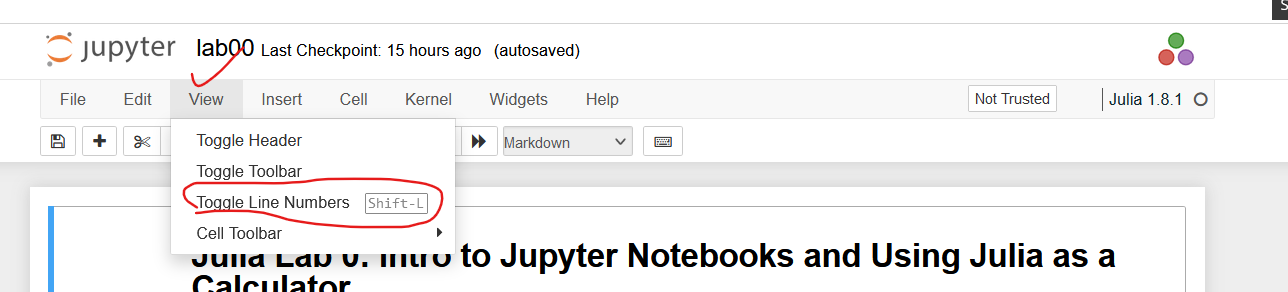
\includegraphics[width=0.9\columnwidth]{graphics/Chap00/VocareumToggleLineNumbers.png}}%
}



\begin{rem} \textbf{(Enable Line numbering)} \texttt{View > Toggle Line Numbers}. In labs and on homework assignments, you will come across instructions which tell you to alter certain lines of your code. You will also need to debug your code based on the errors reported by Julia, which will tell you the line number at which your program failed. 
\end{rem}

If you are in a Jupyter notebook and want to \textbf{create a new cell}, hit the plus sign  \Plus ~in the top banner. The cell will open below the cell in which you last clicked with your cursor (play around with it). This works for HW, LABs, and empty Jupyter notebooks. If you want to try something out, such as rewriting a piece of code without erasing your current code, just open a new cell below the current one, copy and paste in whatever you wish and go to work. To \textbf{remove a cell}, click on it with your cursor, and then click on the scissor symbol \ScissorHollowRight, which is right next to the plus sign \Plus. To \textbf{run a cell}, you hit the run $\blacktriangleright$~\texttt{Run} button on the top banner. On a PC, you can hold \texttt{Shift Enter}. It is worth getting to know the family of buttons on the top banner. Experiment a little! Google a little.\\

\setlength{\fboxrule}{3pt}%
	\centerline{ \fbox{ 
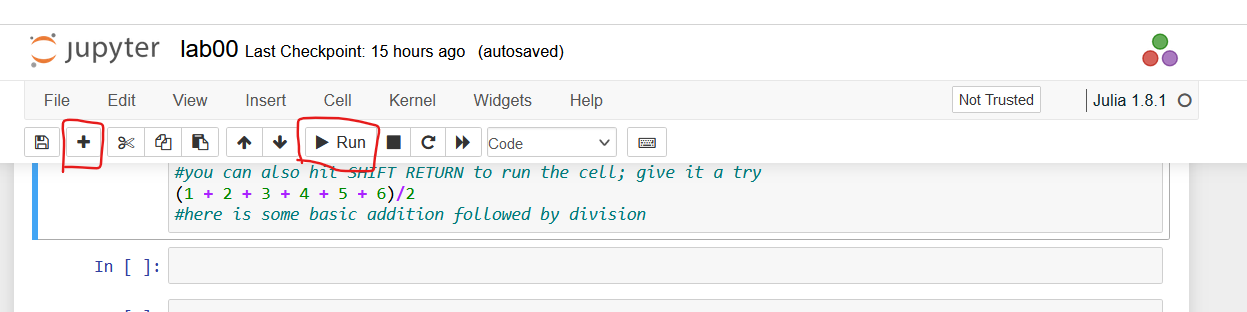
\includegraphics[width=0.9\columnwidth]{graphics/Chap00/VocareumNewCell.png}}%
}

\subsection{Rounding Error}

\begin{lstlisting}[language=Julia,style=mystyle]
#in a code cell, julia will compute and return operations you do inside it
(1 + 2 + 3 + 4 + 5 + 6)/2
#here is some basic addition followed by division
\end{lstlisting}
\textbf{Output} 
\begin{verbatim}
10.5
\end{verbatim}

Computers do arithmetic with a \textbf{finite number} of zeros and ones.  That's easy to accept. Some of the consequences of doing arithmetic with zeros and ones may be hard to accept when you first start programming. Let's take a look, because \textbf{you probably never noticed what is generally called ``rounding error'' when you used a calculator}. 

\begin{lstlisting}[language=Julia,style=mystyle]
# in a code cell, julia will compute and return operations you do inside it
4+7.62
# basic addition
\end{lstlisting}
\textbf{Output} 
\begin{verbatim}
11.620000000000001
\end{verbatim}
Wait a minute, we're pretty good at arithmetic, ``Julia\footnote{The error has nothing to do with the Julia programming language and everything to do with the binary numbers used in a digital computer.}'' got the wrong answer! It's off by $0.000000000000001 =$ 1e-15 or $1 \times 10^{-15}$. In fact, the actual error is 
\begin{lstlisting}[language=Julia,style=mystyle]
# rounding error
(4+7.62) - 11.62
\end{lstlisting}
\textbf{Output} 
\begin{verbatim}
1.7763568394002505e-15
\end{verbatim}
\textbf{You don't need to understand the source of the error to be successful in ROB 101, but you do need to accept that it occurs.} \\

\textbf{(Optional read:)} \emph{In case you are interested, the \textbf{rounding error} comes from the fact that digital computers do calculations in base 2 using a finite number of zeros and ones.} 
\begin{itemize}
    \item By way of background, you are comfortable with the fraction $\frac{1}{3}$ having the infinite decimal expansion 0.3333333\ldots This means that 
    $$\frac{1}{3} = \sum_{k=1}^\infty\frac{3}{10^k} = \frac{3}{10} + \frac{3}{100} + \frac{3}{1000} +  \frac{3}{10000} +  \frac{3}{100000} +\cdots,$$
    where the $\cdots$ means it goes on forever! Hence, it is not possible to represent the number $\frac{1}{3}$ in decimal notation using a finite number of digits between zero and nine. 
    \item In base 3, however, the decimal fraction $\frac{1}{3}$ has the finite expansion $0.1$, while  $\frac{1}{3} + \frac{2}{3^2} = \frac{5}{9} = 0.555555$ in base 10 has the base 3 expansion 0.12. Finally, $\frac{1}{3} + \frac{2}{3^2} + \frac{1}{3^3}= \frac{16}{27} = 0.592592592$ in base 10, but has the base 3 expansion 0.121.
    \item If you have forgotten or never mastered representing numbers in different bases, then don't worry about it. You can simply accept that a number having a finite (exact) expansion in base 10 does not mean it has a finite (exact) expansion in base 2, the number system used in digital computers.
    \item The number 7.62 requires three digits to express in base 10 (decimal numbers), but it takes an \emph{infinite number of digits} in base 2 (binary numbers). Julia is using something like 111.10011110101110000101 as the binary approximation of 7.62, which is roughly 7.61999988555908203125 in decimal, and is ``very close'' to 7.62, but not equal to it. Indeed, 
\begin{align*}
    \overbrace{111}^{7}.\overbrace{10 01111 01011 10000 101}^{\approx 0.62} =& \overbrace{1 \times 2^2 + 1 \times 2^1 + 1 \times 2^0}^{4 + 2 + 1 = 7} +  \overbrace{ 1 \times 2^{-1} + 0 \times 2^{-2}}^{\text{fraction starts here}} +\\
    &  0 \times 2^{-3} + 1 \times 2^{-4} + 1 \times 2^{-5} + 1 \times 2^{-6} + 1 \times 2^{-7} + \\
     &  0 \times 2^{-8} + 1 \times 2^{-9} + 0 \times 2^{-10} + 1 \times 2^{-11} + 1 \times 2^{-12} + \\
     &  1 \times 2^{-13} + 0 \times 2^{-14} + 0 \times 2^{-15} +0 \times 2^{-16} +0 \times 2^{-17} + \\
     &  1 \times 2^{-18} + 0 \times 2^{-19} + 1 \times 2^{-20} \\
     \approx& 7.619 999 885 559 082 031 25 \\
     =& 7 \times 10^{0} + 6 \times 10^{-1} + 1 \times 10^{-2} + 9 \times 10^{-3} +  9 \times 10^{-4} +  9 \times 10^{-5} + \\
     & \vdots \\
    & 2 \times 10^{-15}+ 0 \times 10^{-16}+  3 \times 10^{-17} +  1 \times 10^{-18}  +  2 \times 10^{-19} +  5 \times 10^{-20}, 
\end{align*}
where the symbol $\approx$ means ``approximately equal to''. This explains the error, in case you care. Understanding ``rounding error'' is not important for ROB 101, but eventually, it becomes important for all students of STEM.
\item If a number has a finite representation in either base 2 or base 5, then it will have a finite representation in base 10, simply because 2 and 5 are factors of 10. For example, 
$$\frac{1}{2^k} = \frac{5^k}{2^k 5 ^k} = \frac{5^k}{10 ^k}.$$
If you stare at this for awhile, you will convince yourself that if in binary, a number has $k$ digits after the ``decimal point'' (binary point?), then in decimal, it will have at most $k$ digits after the decimal point. 
\item Because 3 is not a factor of 10, there is no ``reciprocity'' on finite expansions, as we saw with the fraction $1/3$.    
    \end{itemize}


\begin{notation} In case you are curious, the general name for the point ``\textbf{\large .}'' that separates the integer part of a number from the fractional part is \textbf{radix point} \url{https://en.wikipedia.org/wiki/Decimal_separator}. Not everyone uses points to indicate the separator. The French use a comma to separate the integer part of a number from the fractional part and a period to separate powers of ten. And they are not alone in this practice! Your author did a post-doc in Paris back in the 80's, and had a checking account, of course. Getting the commas and periods correct was slightly important when I wrote a check.
\end{notation}

\begin{rem} This web page documents how fractions are handled in various programming languages, including Julia, Matlab, and C++, \url{https://0.30000000000000004.com/}. 
\end{rem}


\subsection{Assignment Operator is Denoted with an Equals Sign}

In mathematics, when we write $x+y+2=3$, we mean the value of the sum of $x$, $y$, and $2$ equals the number $3$. We can ``rearrange'' the equation and write $x + y = 1$ or $x = 1 - y$ without changing what the equation means. \\

In programming, it is very important to understand that the symbol $=$ means \textbf{assignment}. For example, $x=(1 + 2 + 3 + 4 + 5 + 6)/2$ \textbf{assigns} the value 10.5 to the variable $x$. You can now use $x$ in calculations that follow it. It will hold the value 10.5 until you assign something else to it.

\begin{lstlisting}[language=Julia,style=mystyle]
# assigning a value to x
x=(1 + 2 + 3 + 4 + 5 + 6)/2
\end{lstlisting}
\textbf{Output} 
\begin{verbatim}
10.5
\end{verbatim}

\begin{lstlisting}[language=Julia,style=mystyle]
# because we have already assigned x, we can use it in further calculations
y = 3*x
\end{lstlisting}
\textbf{Output} 
\begin{verbatim}
31.5
\end{verbatim}


\begin{lstlisting}[language=Julia,style=mystyle]
# We can update x, using its past value
x = 3*x
\end{lstlisting}
\textbf{Output} 
\begin{verbatim}
31.5
\end{verbatim}

\textbf{The assignment operator does not work like an equals sign.}
\begin{lstlisting}[language=Julia,style=mystyle]
x=x-0.5
\end{lstlisting}
\textbf{Output} 
\begin{verbatim}
31.0
\end{verbatim}
In ``regular'' arithmetic, we could subtract $x$ from both sides of the equation $x=x-0.5$ and arrive at the nonsensical equation, $0=-0.5$. In the computer, you need to think of the left hand side of $x=x-0.5$ as the new value that $x$ will hold. When $x$ appears on the right hand side as well, the computer will use the current value of $x$, which in our case, was $31.5$, perform whatever operations you have specified, and store the new value in $x$. \textbf{In a programming language, $=$ is an assignment operation and not an equals sign.}\\

\begin{rem} \textbf{(Hindsight is 20/20, or the Equals Sign Blues)}
When that first computer programming language was written, there was probably no $\leftarrow$ on the keyboard and hence the notation 
$$ x \leftarrow x+3$$
was not adopted. The left arrow $\leftarrow$ would make a perfectly good assignment operator. In fact, it has been adopted when writing pseudo code \url{https://en.wikibooks.org/wiki/GCSE_Computer_Science/Pseudocode}, which is an informal language, between a human language and a computer language, used for giving the key steps of an algorithm without committing to any particular coding paradigm.
\end{rem}


\subsection{Arithmetic Operations and PEMDAS}

PEMDAS stands for \textbf{P}arentheses, \textbf{E}xponentials, \textbf{M}ultiplication \& \textbf{D}ivision (left to right), \textbf{A}ddition and \textbf{S}ubtraction, the order in which Julia performs operations. While it is fine to memorize this, it is usually better to employ more parentheses than is necessary to make your code easily readable.
\begin{itemize}
    \item Parentheses
\item Exponentials (right to left)
\item Multiplication and Division (left to right)
\item Addition and Subtraction (left to right)
\end{itemize}

\begin{lstlisting}[language=Julia,style=mystyle]
# The symbol ^ means ``raise to the power''
10^(2 + 1)
\end{lstlisting}
\textbf{Output} 
\begin{verbatim}
1000
\end{verbatim}

\begin{lstlisting}[language=Julia,style=mystyle]
# whereas, without parentheses
10^2 + 1
\end{lstlisting}
\textbf{Output} 
\begin{verbatim}
101
\end{verbatim}


\begin{lstlisting}[language=Julia,style=mystyle]
# you can take the power of variables
x = 10 # just to be sure, we set x to a value
x = x^(x^0.5)
\end{lstlisting}
\textbf{Output} 
\begin{verbatim}
1453.0403018990432
\end{verbatim}


% \begin{lstlisting}[language=Julia,style=mystyle]

% \end{lstlisting}
% \textbf{Output} 
% \begin{verbatim}

% \end{verbatim}

\begin{exercise}
Place one (1) set of parentheses in the expression below to make w equal to 30
\begin{lstlisting}[language=Julia,style=mystyle]
#place your parentheses here
w = 2 + 1 + 2 + 7 * 3 
\end{lstlisting}
\end{exercise}

\textbf{Solution:}

\begin{lstlisting}[language=Julia,style=mystyle]
w = 2 + 1 + (2+7)*3 
\end{lstlisting}
\textbf{Output} 
\begin{verbatim}
30.0
\end{verbatim}

\begin{rem} With no parentheses, the result of $w = 2 + 1 + 2 + 7 * 3 $ is $w=26$ because, Julia first does $7 *3=21$ and then performs the addition left to right,  $2 + 1 + 2  + 21 = 26.$

\end{rem}

\begin{exercise}
Place two (2) sets of parentheses in the expression below to make z equal to 7
\begin{lstlisting}[language=Julia,style=mystyle]
#place your parentheses here
z = 2 + 1 + 2 + 7 * 3 + 2 / 10 + 2
\end{lstlisting}
\end{exercise}

\textbf{Solution:}

\begin{lstlisting}[language=Julia,style=mystyle]
z=2 + (1 + (2+7)*3 + 2)/10 + 2
\end{lstlisting}
\textbf{Output} 
\begin{verbatim}
7.0
\end{verbatim}

\begin{rem}
Adding parentheses to someone else's equation is no fun! Your instructor hates those kinds of problems. The take-home point is that parentheses allow you to control the order of computations. If you did not find the solution to the problem on your own, no worries. 
\end{rem}

\begin{rem} With no parentheses, the result of $z = 2 + 1 + 2 + 7 * 3 + 2 / 10 + 2$ is $z=28.2$ because, Julia first does $7 *3=21$ and 2/10 = 0.2, before then performing the addition left to right,  $2 + 1 + 2  + 21 + 0.2 + 2= 28.2.$
\end{rem}



\subsection{Reading an Error Message}

You are going to make lots of errors. Let's make an error on purpose to see what happens. It is assumed that you have not yet defined a value to the variable $r$. If you have used $r$, replace it in the following with something else, like $rr$.

\begin{lstlisting}[language=Julia,style=mystyle]
# A deliberate error
r = r+2
\end{lstlisting}
\textbf{Output} 
\begin{verbatim}
UndefVarError: r not defined

Stacktrace:
 [1] top-level scope
 @ In[15]:2
 [2] eval
   @ ./boot.jl:360 [inlined]
 [3] include_string(mapexpr::typeof(REPL.softscope), mod::Module, code::String,
 filename::String)
   @ Base ./loading.jl:1094
\end{verbatim}

Julia reported that $r$ is an \textbf{undefined variable} via the statement \texttt{UndefVarError: r not defined}. That's cool, you now know the name of the problematic variable and the nature of the problem. You were next told in which cell of your Jupyter notebook the error occurred, here it was input cell 15, and the line number of the cell in which the error occurred, here it was line 2. You can see all of this from the line \texttt{@ In[15]:2}. The other parts of the error message are helpful for a Julia professional, but not so much for us. Once again, the key parts of the error message are \newline
\textcolor{blue}{\bf Stacktrace:}\newline
 \textbf{[1] top-level scope} \newline
\textcolor{red}{\bf @ In[15]:2 ~~$\leftarrow$ gave the Jupyter Cell number and the line number in the cell where the error occurred.} When you compose more complicated notebooks, the Cell number may be further up in your jupyter notebook, possibly where you define a new function. Julia's error messages can be called lot's of things, cryptic and arcane would be two of the nicer ones. Oh well! \textbf{Always look for the line that has \texttt{In[ some cell number ]: some line number } to get started on locating your error.} And of course, have line numbering turned on.


\section{Standard Bulit-in Functions}

As you can imagine, Julia has many built-in functions, more than a standard calculator will have. Here are a few,
\begin{itemize}
\item abs() \#absolute value
\item sin(), cos(), tan(), asin(), acos(), atan()  \#many more trigonometric functions
\item sqrt() \#square root
\item exp()  \#natural exponential $e^x$
\item log() \#natural logarithm
\item round() \#rounds to nearest integer
\item ceil() \#rounds up to the nearest integer
\item floor() \#rounds down to the nearest integer
\item trunc() \#chops off anything beyond the decimal point
\end{itemize}
and so many more \url{https://docs.julialang.org/en/v1/manual/mathematical-operations/}. They key thing with a programming language is that you can expand the language by writing your own functions. In later labs, we will definitely build our own functions in ROB 101. \\

It is enough to scan the following. If you want to enter them into the lab0 notebook, feel free. Recall that LABS are not graded and you do not submit them to us. LABS are to help you learn Julia for use in the HW sets and the Projects.\\


\begin{lstlisting}[language=Julia,style=mystyle]
cos(3*pi/4) #It assumes radians and not degrees
\end{lstlisting}
\textbf{Output} 
\begin{verbatim}
-0.7071067811865475
\end{verbatim}

\begin{lstlisting}[language=Julia,style=mystyle]
0.5-cos(3*pi/4)^2  #In perfect math, the answer should be zero
\end{lstlisting}
\textbf{Output} 
\begin{verbatim}
1.1102230246251565e-16
\end{verbatim}

\begin{rem}
$1.1102230246251565e$-$16 \approx 2 ^{-53}$. Hence, in binary, that is 52 zeros after the ``radix point'' followed by a 1. That's pretty close to zero!
\end{rem}

\begin{lstlisting}[language=Julia,style=mystyle]
exp(log(2))  # remember e ^ log(x) = x
\end{lstlisting}
\textbf{Output} 
\begin{verbatim}
2.0
\end{verbatim}

\begin{lstlisting}[language=Julia,style=mystyle]
log10(10^3) # log base 10 instead of the natural log, which is base e
\end{lstlisting}
\textbf{Output} 
\begin{verbatim}
3.0
\end{verbatim}
\begin{lstlisting}[language=Julia,style=mystyle]
round(1.5)    #Goes to the nearest integer. Which way will 1.5 go? It's quite arbitrary.
\end{lstlisting}
\textbf{Output} 
\begin{verbatim}
2.0
\end{verbatim}

\begin{lstlisting}[language=Julia,style=mystyle]
# ceil is short for ceiling, which is above you, typically,
# while floor is below you.

ceil(1.5)    #note that ceil and floor always round "predictably"
\end{lstlisting}
\textbf{Output} 
\begin{verbatim}
2.0
\end{verbatim}

\begin{lstlisting}[language=Julia,style=mystyle]
floor(1.5)     #for instance, floor always returns a number less than or equal 
              #to the input argument, while
              #ceil is greater or equal to the its input argument
\end{lstlisting}
\textbf{Output} 
\begin{verbatim}
1.0
\end{verbatim}


\section{How to ``Reboot'' your Jupyter Notebook}
\label{sec:Reboot}

From time to time, your jupyter notebook will freeze up or code will not run properly. In these cases, you need to do the equivalent of ``rebooting your laptop''. Here is how to do it. \\


\setlength{\fboxrule}{3pt}%
	\centerline{ \fbox{ 
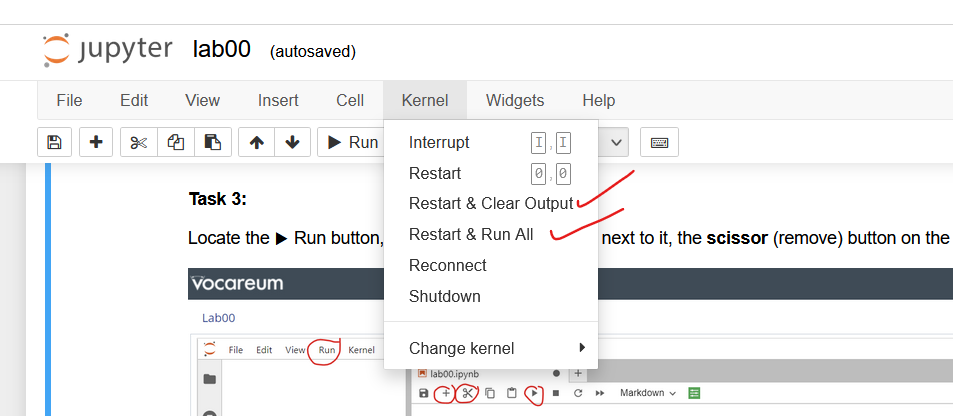
\includegraphics[width=0.5\columnwidth]{graphics/Chap00/VocareumLab00RestartKernel.png}}%
}


\begin{itemize}
    \item Click on the Kernel tab, to get the above dropdown menu. Click on the \texttt{Restart \& Clear Output} \textbf{or} \texttt{Restart \& Run All}.
    \item \textcolor{blue}{\bf Neither of these erases any code in your Input Cells. Your work is safe! }
    \item \texttt{Restart \& Clear Output} Stops and restarts the program that is running your notebook and clears all of the output cells. You then need to start from the top cell in your notebook (or other relevant location) and re-run each cell to redefine your variables because \textbf{the value of each variable has been ``erased''}. Once again, all of your code is still there. 
    \item \texttt{Restart \& Run All} does all of the above and re-runs every cell in your notebook automagically (not a typo). You'll have to experiment with these two options to see which one you like best. 
\end{itemize}

\textcolor{red}{\bf Sometimes the above is not enough and you need a ``nuclear option''.} \textbf{The following will create a brand-new notebook, with all of your work erased. Yes. You have to start all over again!} Step 1, if the system is not hung up too badly,  is to hit the file tab, look for \texttt{Download as}, and select \texttt{Save as notebook}. If the system is hung up badly and you cannot download your current notebook, then in a different browser (e.g., if you are using Chrome, go to Edge) and access the ROB 101 site and fetch a fresh notebook.\\

\setlength{\fboxrule}{3pt}%
	\centerline{ \fbox{ 
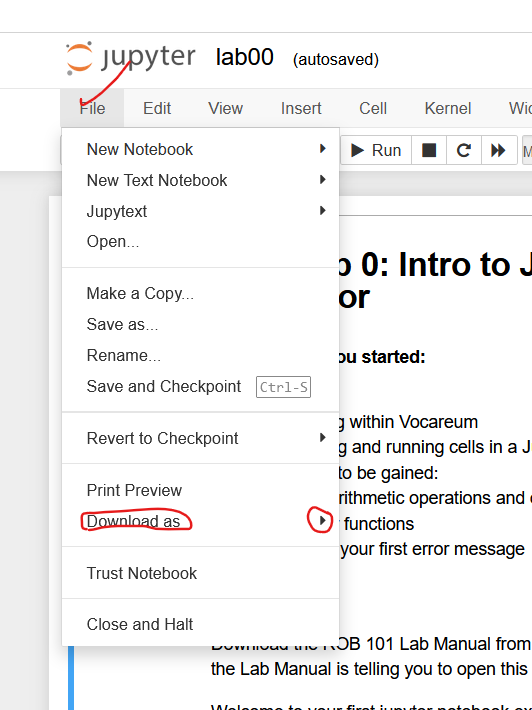
\includegraphics[width=0.3\columnwidth]{graphics/Chap00/VocareumDownloadFile.png}
}}
\vspace*{.2cm}

Step 2 is to hit the \textbf{End Lab and Reset} buttons. Be patient. It can take some time to close all of the related processes. This will open up a fresh assignment, with any previous work \textbf{Completely Erased}. Copy and paste in relevant work from your previous file, if possible. \textcolor{red}{\bf Personally, I do not close my previously opened file until I am sure that I do not need to copy any lines of code from it.} You'll arrive at your own file management etiquette!\\

\setlength{\fboxrule}{3pt}%
	\centerline{ \fbox{ 
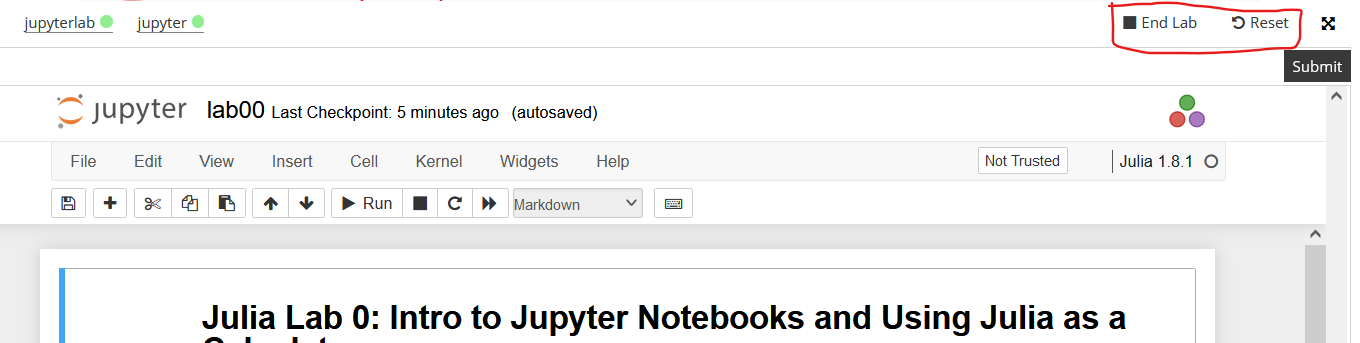
\includegraphics[width=0.9\columnwidth]{graphics/Chap00/VocariumNuclearOption.png}}%
}
\begin{center}
\fcolorbox{red}{yellow}{%
    \minipage[t]{\dimexpr0.9\linewidth-2\fboxsep-2\fboxrule\relax}
        \large \bf 
Sometimes, you may find yourself with a screen that is different than what you expect. Don't panic, just hit the \texttt{jupyter} button at the top and everything will return to normal!
    \endminipage}
    \end{center}


\vspace*{.2cm}

\setlength{\fboxrule}{3pt}%
	\centerline{ \fbox{ 
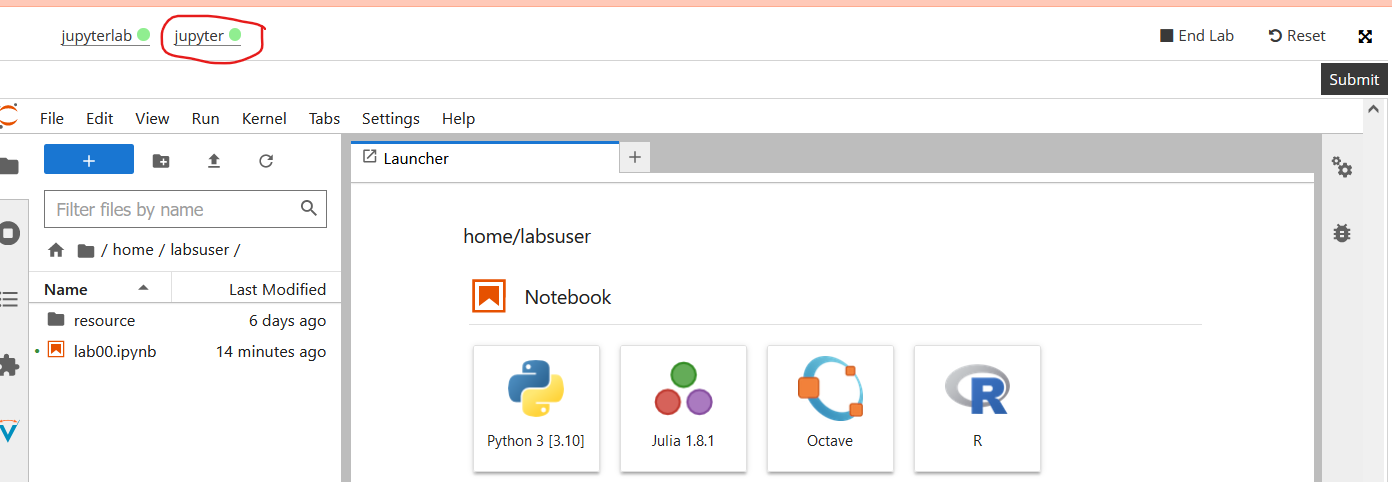
\includegraphics[width=0.9\columnwidth]{graphics/Chap00/VocareumJupyterTab.png}}%
}


\section{Pro Tip: Hit the Save Button!}

It's a good idea to ensure that your work is saved as you go. Your author hits the \texttt{CNTRL-S} key frequently on a Window's Machine. You can also use the \texttt{Disc} icon as shown below.\\

\setlength{\fboxrule}{3pt}%
	\centerline{ \fbox{ 
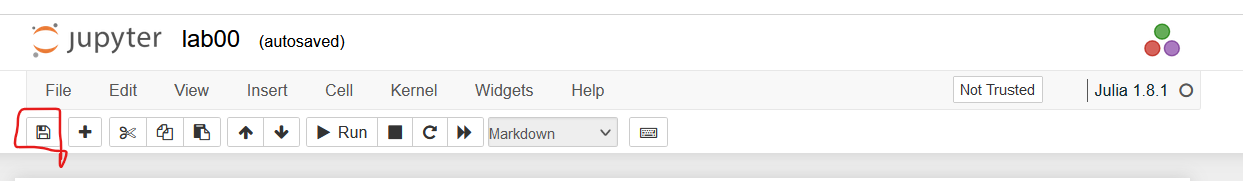
\includegraphics[width=0.9\columnwidth]{graphics/Chap00/VocareumSaveButton.png}}%
}


\section{Julia is not Working. What can I do?}

Here are some suggestions, in the recommended order of use. 
\begin{itemize}

    \item Hit the \textbf{End Lab} button in the upper right corner. That is supposed to give you a new session with your solutions intact, meaning, none of your coding is erased. You will have to re-run your cells as the results of your answers are erased. Once again, no work is lost. \textcolor{red}{\bf Do not yet hit the reset button.}

    \item Next, check on Piazza to see if anyone else is having the same problem. A fix may be posted.

    \item If not, \textcolor{blue}{\bf a common reason that Julia stops working is that your Canvas login has expired}. Say you had juliahwXX open at 1 AM, go to bed, and start again at noon. Canvas is likely to have blocked your credentials without closing the open window/tab. When Canvas does that, all tools connected to Canvas are no longer accessible. The solution is 
    \begin{itemize}
    \item Keep the current copy of juliahwXX open. 
    \item Exit Canvas and log back in or just open up a fresh Canvas login to ROB 101 in a new tab, or better yet, a different browser (if you were in Chrome, try Edge or Firefox).
    \item Re-open juliahwXX
    \item Copy over any work that was not saved. Usually, that will be very little because you will have followed the Pro-Tip and hit the save button frequently! 
    \end{itemize}

    \item If the above does not work, please post on Canvas under help!help! and under Julia. The IAs and Instructors can post on the Vocareum forum that we need HELP and we need it NOW!

    \item It's late at night and you are desperate. No one is around to respond to your Piazza post. You are frustrated and all alone. It's good to try once again the \textbf{End Lab} button in the upper right corner. Wait two minutes and launch Canvas in a different browser, go to modules, invoke any magic incantations that have saved you in the past, maybe the one that got you accepted into Michigan, and hope for the best. When this fails, well, then, the ``Nuclear Option'' in Chapter~\ref{sec:Reboot} is likely your best bet. \textcolor{red}{\bf It will erase all of your work. You will be given a pristine notebook.} User discretion is advised. 
\end{itemize}

\section{My Submit Button has Disappeared! What do I do?}

This happens rarely, but it can be very disconcerting. Fortunately, there are a few easy things to try.
\begin{itemize}

    \item If you can see the \textbf{stop lab} button at the top right, hit it.  This will NOT erase your work. Wait a bit. You should be given a chance to re-open the notebook. Hit submit as normal. If that does not work...
    
    \item Close your HW or Project. Logout of Canvas. Log back into Canvas. Open your jupyter notebook. Normally, this does it, but if not ...

    \item Go to \url{https://labs.vocareum.com/main/main.php} and log in to your account on Vocareum using your email address. You will likely not know your password, click on \textbf{forgot password}, enter the email address being used by Canvas, and have Vocareum send you a password reset. After logging in, click on \textit{ROB 101 Computational Linear Algebra}, click on the jupyter file in question, and then click the submit button as normal.


\end{itemize}

\section{(Optional Read) Additional Julia Resources}

\begin{itemize}

    \item \href{https://web.mit.edu/julia_v0.6.2/julia/share/doc/julia/html/en/index.html}{Complete Julia Documentation}

    \item \href{https://web.mit.edu/julia_v0.6.2/julia/share/doc/julia/html/en/manual/linear-algebra.html#Linear-algebra-1}{Linear Algebra}
    \item  \href{https://web.mit.edu/julia_v0.6.2/julia/share/doc/julia/html/en/manual/noteworthy-differences.html#Noteworthy-differences-from-MATLAB-1}{Noteworthy Differences from Matlab}
     \item  \href{https://web.mit.edu/julia_v0.6.2/julia/share/doc/julia/html/en/manual/noteworthy-differences.html#Noteworthy-differences-from-C/C-1}{Noteworthy Differences from C++}

     \item \href{https://web.mit.edu/julia_v0.6.2/julia/share/doc/julia/html/en/manual/faq.html}{FAQ for Advanced Users of Julia}
\end{itemize}


\section{(Optional Read) Why was Julia Created?}


The following material is from \url{https://juliadatascience.io/julia_accomplish}: 
``We are greedy: we want more. We want a language that’s open source, with a liberal license. We want the speed of C with the dynamism of Ruby. We want a language that’s homoiconic, with true macros like Lisp, but with obvious, familiar mathematical notation like Matlab. We want something as usable for general programming as Python, as easy for statistics as R, as natural for string processing as Perl, as powerful for linear algebra as Matlab, as good at gluing programs together as the shell. Something that is dirt simple to learn, yet keeps the most serious hackers happy. We want it interactive and we want it compiled.''\\

You can find many more reasons \href{https://web.mit.edu/julia_v0.6.2/julia/share/doc/julia/html/en/manual/introduction.html#man-introduction-1}{here}.



% \begin{lstlisting}[language=Julia,style=mystyle]

% \end{lstlisting}
% \textbf{Output} 
% \begin{verbatim}

% \end{verbatim}

% \section{(Optional Read) Useful Tip: Hit the Save Button!}

% It's a good idea to ensure that your work is saved as you go. Your author hits the \texttt{CNTRL-S} key frequently on a Window's Machine. You can also use the \texttt{Disc} icon as shown below.\\

% \setlength{\fboxrule}{3pt}%
% 	\centerline{ \fbox{ 
% 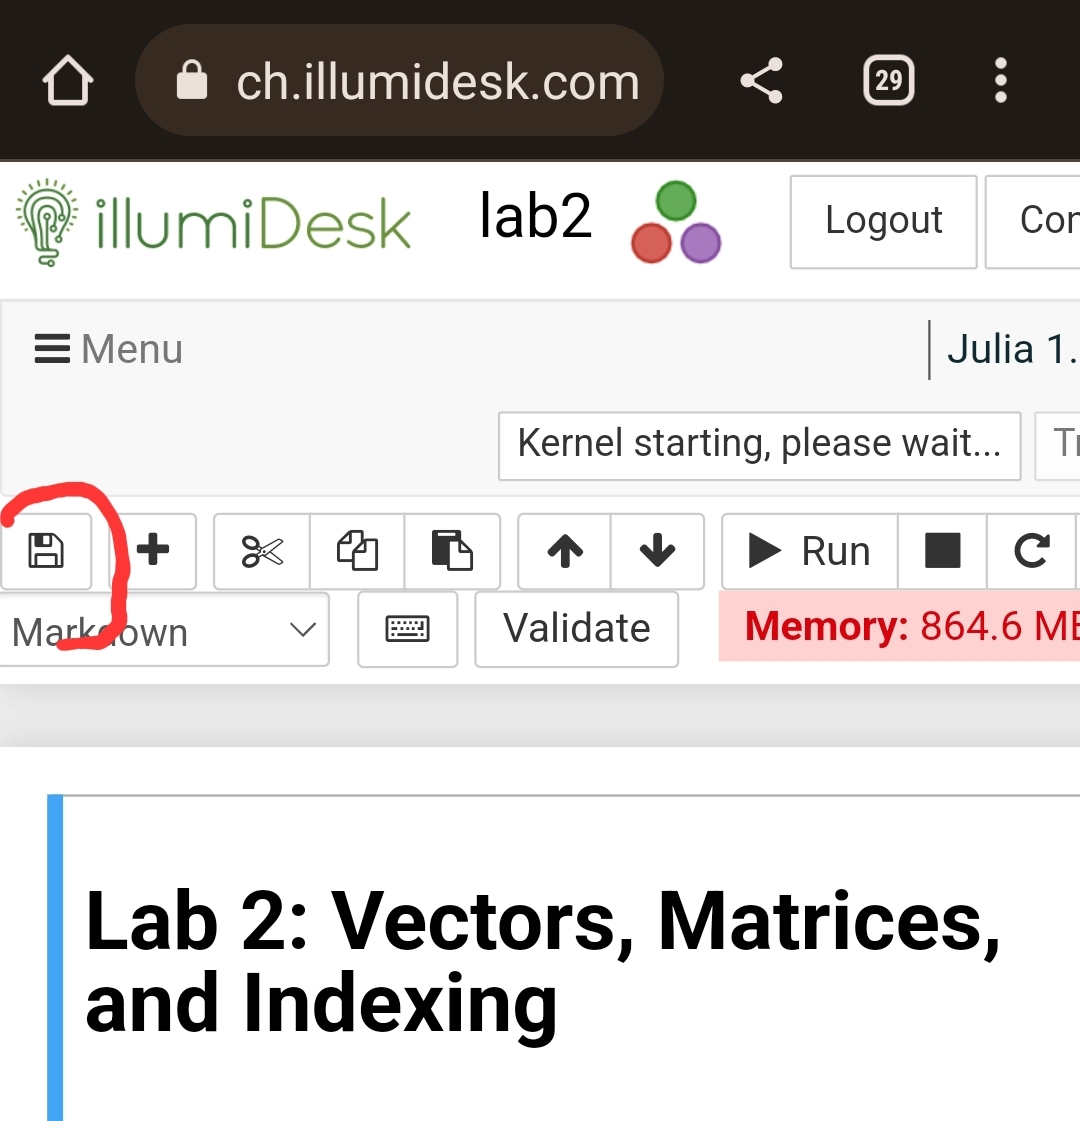
\includegraphics[width=0.9\columnwidth]{graphics/Chap00/Save_Button.jpg}}%
% }


% \begin{lstlisting}[language=Julia,style=mystyle]

% \end{lstlisting}
% \textbf{Output} 
% \begin{verbatim}

% \end{verbatim}



% \begin{lstlisting}[language=Julia,style=mystyle]

% \end{lstlisting}
% \textbf{Output} 
% \begin{verbatim}

% \end{verbatim}




% \begin{lstlisting}[language=Julia,style=mystyle]

% \end{lstlisting}
% \textbf{Output} 
% \begin{verbatim}

% \end{verbatim}



% \begin{lstlisting}[language=Julia,style=mystyle]

% \end{lstlisting}
% \textbf{Output} 
% \begin{verbatim}

% \end{verbatim}


% \begin{lstlisting}[language=Julia,style=mystyle]

% \end{lstlisting}
% \textbf{Output} 
% \begin{verbatim}

% \end{verbatim}



% \begin{lstlisting}[language=Julia,style=mystyle]

% \end{lstlisting}
% \textbf{Output} 
% \begin{verbatim}

% \end{verbatim}




% \begin{lstlisting}[language=Julia,style=mystyle]

% \end{lstlisting}
% \textbf{Output} 
% \begin{verbatim}

% \end{verbatim}



% \begin{lstlisting}[language=Julia,style=mystyle]

% \end{lstlisting}
% \textbf{Output} 
% \begin{verbatim}

% \end{verbatim}

\chapter{Julia Lab 1: Variable Types, Plotting a Function, and Creating Arrays}
\label{chap:Lab1}

\section*{Learning Objectives}

\begin{itemize}
\item  Some basic computing constructs
\item  Moving beyond a graphical calculator
\item Getting started with debugging code in Julia
\end{itemize}

\section*{Outcomes} 
\begin{itemize}
\item Types of variables in Julia
\begin{itemize}
    \item Int64
    \item Float64
    \item Char
    \item String
    \end{itemize}
\item Building arrays
\item Declaring and plotting functions
\item Applying functions to arrays via broadcasting
\item First appearance of $n$-element Vector\{\texttt{Type}\} and $n \times m$
Matrix\{\texttt{Type}\}
\item Commenting out lines of code
\end{itemize}

\vspace*{1cm}

\textbf{Either download Lab1 from our Canvas site or open up a Jupyter notebook so that you can enter code as we go. It is suggested that you have line numbering toggled on.}  

\newpage

\section{Variable Types}

``A data \textbf{Type} or simply type is an attribute of data which tells the [computer] how the programmer intends to use the data \url{https://en.wikipedia.org/wiki/Data_type}". Computers have a limited amount of memory (zeros and ones) available to represent a number. If the computer knows that the number does not require a decimal point (as in -7, 0, 1, 45, etc,) then it can store it very compactly and hence store enormously large numbers of the \texttt{Int64 TYPE}. If the number requires a decimal to express it properly (such as pi, sqrt(2), 0.6) then Julia will store it in a different format. Mostly, Julia is able to handle the memory needs of our code without our help, because we tell Julia in advance the memory needs of our variables. \\

Everything in Julia has a \texttt{Type}. We will mostly use variables with these 4 \texttt{Type}
\begin{enumerate}
        \renewcommand{\labelenumi}{(\alph{enumi})}
        \setlength{\itemsep}{.1cm}
    \item \texttt{Int64}
    \item \texttt{Float64}
    \item \texttt{Char}
    \item \texttt{String}
\end{enumerate}

\texttt{\bf Int64} is used for integers or whole numbers, in other words, ...-3, -2, -1, 0, 1, 2, 3, ... The 64 refers to the number of 'bits', 0s and 1s, that are used to represent the number and its sign. The sign takes 1 bit, leaving 63 for the number. It is possible to represent numbers from $-2^{63}$ to $2^{63} - 1$. These are enormous values.\\

    
   \begin{figure}[hbt!]%
	\centering
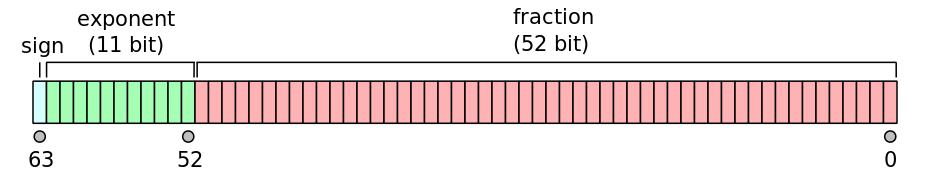
\includegraphics[width=0.75\columnwidth]{graphics/Chap02/FloatingPoint.png}
    \caption[]{ (Optional Read) Explanation from \url{https://en.wikipedia.org/wiki/Double-precision_floating-point_format} on how the bits used to represent a double-precision Floating Point number are organized in a computer.}
    \label{fig:FloatingPoint}
\end{figure} 


\texttt{\bf Float64} Floating point is computer speak for numbers that require decimal points, such as 1.414. Figure~\ref{fig:FloatingPoint} explains (optional read) why larger numbers can be stored in \texttt{Int64} than in \texttt{Float64}. We mostly do not care about this in ROB 101. We will primarily use floating point variables. But sometimes Julia really wants an integer variable and will throw a ``\texttt{Type Error}'' when you get it wrong. If you are not aware that all variables have a \texttt{Type}, then you will be at a loss to understand your mistake. \\

\texttt{\bf Char} is used to store characters, such as letters, numbers, or symbols. If you dig into Julia, you can learn how to use Chinese characters, Hebrew characters, Greek letters, and more. You place characters between single ` \hspace*{.3cm} ' marks, such as \texttt{x = `A'}.\\

\texttt{\bf String} is used for a sequence of characters in a single line. This could be a word, or a sentence, or even a number that is placed between double quote marks  ``\hspace*{.3cm}'', such as \texttt{myPlotTitle = ``My \#1  Plot in Julia''}.

\begin{rem}
Julia only prints out the last line in a cell that produces a result (it does not count a comment sign \# as a result). To cause other values to print to the screen, use the \texttt{@show} command. To verify (or learn) the \texttt{Type} of a variable, use the \texttt{typeof} command.
\end{rem}

% We will also use **TYPES** that are collections of the above types of variables, 
% - **Array** a collection of values that can be Int64, Float64, Char, String, etc.
% - **Vector** special kind of "one-dimensional'' array
% - **Matrix** special kind of array that can have many "dimensions''



\begin{lstlisting}[language=Julia,style=mystyle]
# Run me
w = 33
x = sqrt(2)
y = 'A'
z = "Oh oh, what I have I done!"
\end{lstlisting}
\textbf{Output} 
\begin{verbatim}
"Oh oh, what I have I done!"
\end{verbatim}



\begin{lstlisting}[language=Julia,style=mystyle]
# Run me
@show w = 33
@show x = sqrt(2)
@show y = 'A'
z = "Oh oh, what I have I done!"
\end{lstlisting}
\textbf{Output} 
\begin{verbatim}
w = 33 = 33
x = sqrt(2) = 1.4142135623730951
y = 'A' = 'A'
"Oh oh, what I have I done!"
\end{verbatim}

You could have added an \texttt{@show} command on $z$ as well. 
\begin{lstlisting}[language=Julia,style=mystyle]
@show typeof(w)
@show typeof(x)
@show typeof(y)
@show typeof(z)
\end{lstlisting}
\textbf{Output} 
\begin{verbatim}
typeof(w) = Int64
typeof(x) = Float64
typeof(y) = Char
typeof(z) = String

String
\end{verbatim}

\begin{rem}
 While Julia \url{https://docs.julialang.org/en/v1/base/numbers/#Standard-Numeric-Types} has a lot of number \texttt{TYPES}, it does not have all of the possible categories of numbers that mathematicians use, \url{https://youtu.be/5TkIe60y2GI}. In addition to \texttt{Int64} and \texttt{Float64}, we'll use from to time \texttt{Complex64}. 
\end{rem}

\section{Creating Simple Functions}

One of the main points of programming is the creation of new functions. Here, we'll learn the simplest way to create a function in Julia and then how to plot a graph of the function.

\begin{lstlisting}[language=Julia,style=mystyle]
f(x) = 5x^2 + 2x - 4  # this is too easy
\end{lstlisting}
\textbf{Output} 
\begin{verbatim}
f (generic function with 1 method)
\end{verbatim}

Note that we used \textbf{integer} coefficients when we composed the function.  
We can now evaluate the function at any point. Let's see what \texttt{Type} of variable is returned

\begin{lstlisting}[language=Julia,style=mystyle]
@show f(3)
@show f(3.0)
@show f(-pi)
\end{lstlisting}
\textbf{Output} 
\begin{verbatim}
f(3) = 47
f(3.0) = 47.0
f(-pi) = 39.06483669826721
39.06483669826721
\end{verbatim}
The first one is clearly \texttt{Int64} (there is no decimal point) and the other two are \texttt{Float64}. Next, we'll modify the function and make at least one of the coefficients a decimal number. All of the outputs are now type \texttt{Float64}.

\begin{lstlisting}[language=Julia,style=mystyle]
f(x) = 5.0x^2 + 2x - 4  # this is way too easy
@show f(3)
@show f(3.0)
f(-pi)
\end{lstlisting}
\textbf{Output} 
\begin{verbatim}
f(3) = 47.0
f(3.0) = 47.0
39.06483669826721
\end{verbatim}

\section{Very Basic Plotting}
\label{sec:basicPlotting}

\textbf{Rich source of plotting examples:} \url{https://gist.github.com/gizmaa/7214002} \\

\textbf{``Tutorial'' for plotting in Julia:} \url{https://docs.juliaplots.org/latest/tutorial/}\\

Julia attempts to avoid filling the memory of your computer with functionality that you do not intend to use. It does that through the use of \textbf{packages}, which are collections of useful functions designed around a single theme, such as plotting (package is called Plots), random numbers (package is called Random), or linear algebra (package is called LinearAlgebra). We have pre-loaded a bunch of packages into the ROB 101 Julia installation. The process of accessing packages is a bit different if you are working in a personal Julia installation versus the course site; we'll give both methods. In the course site, 
\begin{lstlisting}[language=Julia,style=mystyle]
# Turning on the plotting functions
using Plots
gr()
\end{lstlisting}
\textbf{Output} 
\begin{verbatim}
Plots.GRBackend()
\end{verbatim}
while if you are in a personal installation of Julia, do this
\begin{lstlisting}[language=Julia,style=mystyle]
# For a personal installation the first time you use a package
using Pkg
Pkg.add("Plots")
# After the first time, you just need to run these two commands
using Plots
gr()
\end{lstlisting}
\textbf{Output} 
\begin{verbatim}
Plots.GRBackend()
\end{verbatim}

We assume the function $f$ has already been defined. Here we are using $f(x) = 5.0x^2 + 2x - 4 $

\begin{lstlisting}[language=Julia,style=mystyle]
# Run me
# now, we can use the plot() function
plot(f, -5, 5, legend=false)  #f will be plotted for x varying from -5 to 5
\end{lstlisting}

\textbf{Output} 

	\begin{center}
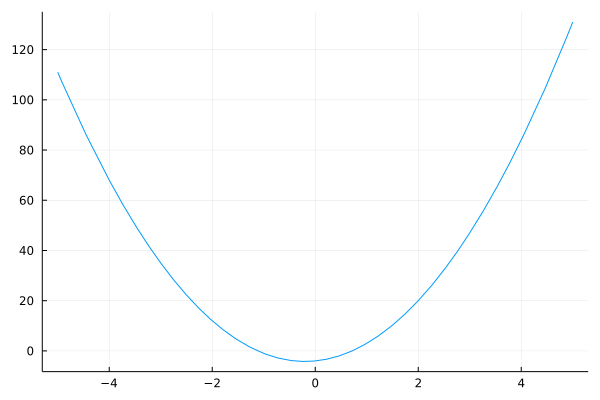
\includegraphics[width=0.5\columnwidth]{graphics/Chap02/Lab01_QuadraticNoLabels.png}
\end{center}

We can add labels to the plot
\begin{lstlisting}[language=Julia,style=mystyle]
plot!(xlabel = "x", ylabel = "y") # plot! modifies the previous plot
\end{lstlisting}

\textbf{Output} 

	\begin{center}
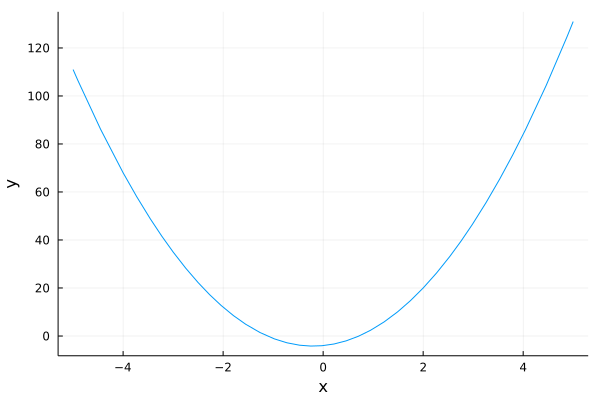
\includegraphics[width=0.5\columnwidth]{graphics/Chap02/Lab01_QuadraticWithLabels.png}
\end{center}


We can put all the commands in one line if we want
\begin{lstlisting}[language=Julia,style=mystyle]
# Run me
xmin=-5
xmax = 5
# You can add a bunch of stuff in one command line, if you want....
plot(f, xmin, xmax, xlabel = "x", ylabel = "y", legend = false) 
\end{lstlisting}

\textbf{Output} 

	\begin{center}
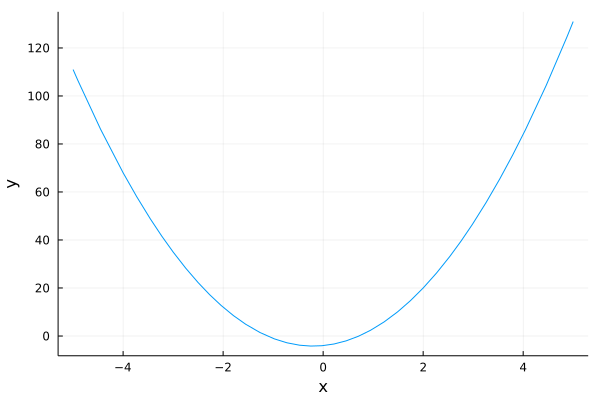
\includegraphics[width=0.5\columnwidth]{graphics/Chap02/Lab01_QuadraticWithLabels.png}
\end{center}



\begin{lstlisting}[language=Julia,style=mystyle]
# Run me to see how to have two functions on the same plot
f(x) = .1x^3 + 2
g(x) = x^2*sin(3*x) 
xmin = -2*pi
xmax = 2 *pi
titre = "Another Passable but not so Aesthetic Plot"
plot(f, xmin,xmax, title=titre, linewidth=3) 
# If you leave off the ! (bang), then the previous plot is erased and
# a new one is started. Try it.
plot!(g, xmin,xmax, title=titre, linewidth=3) #plot bang, it's kind of joyous!
println("Every point where the graphs of f and g cross is a solution of the equation f(x) - g(x) = 0")
plot!(xlabel = "x", ylabel = "y") # plot! modifies the previous plot
# png("Lab01_TwoFunctionsSameGraph") #Creates a png of the graph, uncomment to use
\end{lstlisting}
\textbf{Output} 
\begin{verbatim}
Every point where the graphs of f and g cross is a solution of the equation f(x) - g(x) = 0
\end{verbatim}
	\begin{center}
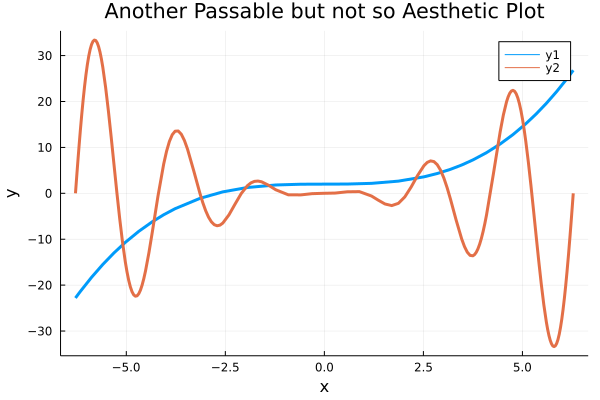
\includegraphics[width=0.5\columnwidth]{graphics/Chap02/Lab01_TwoFunctionsSameGraph.png}
\end{center}

\begin{lstlisting}[language=Julia,style=mystyle]
# Run me to see how to place two functions on the same plot
f(x) = .1x^3 + 2
g(x) = x^2*sin(3*x) 
xmin = -2*pi
xmax = 2 *pi
titre = "Another Passable but not so Aesthetic Plot"
plot([f,g], xmin,xmax, title=titre, linewidth=3) 
println("Every point where the graphs of f and g cross is a solution of the equation f(x) - g(x) = 0")
plot!(xlabel = "x", ylabel = "y") # plot! modifies the previous plot
\end{lstlisting}
\textbf{Output}   Same as from the previous cell.\\

Plotting in Julia is a bit awkward, in your instructor's opinion. We will mostly give you the plotting commands throughout the term. We'd rather you focus on other aspects of coding that are common to most programming languages. \\

\begin{center}
\fbox{ 
\textbf{To learn more about plotting in Julia:}  \url{https://docs.juliaplots.org/latest/tutorial/}}
\end{center}

\section{Creating Arrays}

An \textbf{array} ``is a data structure, which can store a fixed-size collection of elements of the same data type. An array is used to store a collection of data, but it is often more useful to think of an array as a collection of variables of the same type.'' \url{https://www.tutorialspoint.com/computer_programming/computer_programming_arrays.htm}. See also \url{https://press.rebus.community/programmingfundamentals/chapter/arrays-and-lists/}.\\

We will mostly be creating arrays with elements that are one of the following \texttt{Types}:
\begin{enumerate}
        \renewcommand{\labelenumi}{(\alph{enumi})}
        \setlength{\itemsep}{.1cm}
    \item \texttt{Int64}
    \item \texttt{Float64}
    \item \texttt{String}
\end{enumerate}

We'll first build an array with elements in a single row. 
\begin{lstlisting}[language=Julia,style=mystyle]
# Run me to create an array of 10 numbers
# a Matrix is one kind of array
# 1 x 10 Matrix{Int64} means it has one row and ten columns, 
# with each entry of TYPE Int64
myArray = [1 2 3 4 5 6 7 8 9 10]
\end{lstlisting}
\textbf{Output} 
\begin{verbatim}
1×10 Matrix{Int64}:
 1  2  3  4  5  6  7  8  9  10
\end{verbatim}

Note that in Julia, what we call a \textbf{row vector} in lecture is being called a $1 \times n$ matrix, where in this case $n=10$ because there are 10 entries in the vector. Note that Julia is confirming the data \texttt{Type} for us, $ 1 \times 10 ~\text{\rm  Matrix}\{\bf Int64\}.$ Each entry of the array has data type \texttt{\bf Int64}. However, if we change even one of the entries to \texttt{\bf Float64}, then \textbf{all of the entries} become \texttt{\bf Float64}, as shown below.

\begin{lstlisting}[language=Julia,style=mystyle]
# Run me to create an array of 10 numbers
# We change one of the values to a number of TYPE Float64, 
# and leave the rest as TYPE Int64. Watch what happens
# 
# 1 x 10 Matrix{Float64} means it has one row and ten columns, 
# with each entry of TYPE Float64
println("All elements assume TYPE Float64")
myArray = [1.0 2 3 4 5 6 7 8 9 10]
\end{lstlisting}
\textbf{Output} 
\begin{verbatim}
All elements assume TYPE Float64

1 x 10 Matrix{Float64}:
 1.0  2.0  3.0  4.0  5.0  6.0  7.0  8.0  9.0  10.0
\end{verbatim}

In Julia, arrays that are arranged in a column are called \textbf{Vectors}. What we call a \textbf{column vector} in lecture is simply a vector in Julia because Julia does not have two kinds of vectors. Julia only has column vectors and because of that, it is redundant to use the adjective ``column''. OK! In lecture, it is not redundant to specify column vs row when talking about a vector.\\

In Julia, when you use \textbf{commas} or \textbf{semicolons} to separate the elements of an array to form a ``column vector'', it is automatically declared as a \textbf{Vector}. Below, we build a 
5-element \texttt{Vector\{\bf Float64\}}. We used semicolons. You can replace the semicolons with commas and check that you get the same result. You cannot mix, however, commas and semicolons in the same array. 

\begin{lstlisting}[language=Julia,style=mystyle]
# Run me to create an array of 5 numbers
# arranged as a column
# 5-element Vector{Float64} means it has five elements, 
# each with value of TYPE Float64
#
println("You can separate the elements by commas OR by semicolons. This is different than MATLAB.")
myArray = [1.0; 2; 3; 4; 5]
\end{lstlisting}
\textbf{Output} 
\begin{verbatim}
You can separate the elements by commas OR by semicolons. This is different than MATLAB.

5-element Vector{Float64}:
 1.0
 2.0
 3.0
 4.0
 5.0
\end{verbatim}

You can build vectors with elements that have type \texttt{String}.

\begin{lstlisting}[language=Julia,style=mystyle]
# Run me to create an array with names in it
# 6-element Vector{String} means it is a column vector with 
# elements of TYPE String. Note that we used commas this time.
animalsVector = ["lemur", "elephant", "tiger", "panda", "zebra", "cuttlefish"]
\end{lstlisting}
\textbf{Output} 
\begin{verbatim}
6-element Vector{String}:
 "lemur"
 "elephant"
 "tiger"
 "panda"
 "zebra"
 "cuttlefish"
\end{verbatim}

You can also create $1 \times n$ matrices with elements that have type \texttt{String}.

\begin{lstlisting}[language=Julia,style=mystyle]
# Run me to see what happens when one uses spaces to separate the elements
animalsVector = ["lemur" "elephant" "tiger" "panda" "zebra" "cuttlefish"]
\end{lstlisting}
\textbf{Output} 
\begin{verbatim}
1×6 Matrix{String}:
 "lemur"  "elephant"  "tiger"  "panda"  "zebra"  "cuttlefish"
\end{verbatim}

\begin{exercise}
Build three arrays, each with five elements
\begin{enumerate}
    \item myArray01 is a 1 x 5 matrix with entries of TYPE Float64
    \item myArray02 is a 5-element vector with entries of TYPE Float64
    \item myArray03 is a 5-element vector with entries of TYPE String
\end{enumerate}
\end{exercise}
\textbf{Solution}


\begin{lstlisting}[language=Julia,style=mystyle]
# Place your answers here
@show myArray01 = [1/3 11 4 2^(0.5) 7.62]
@show myArray02 = [1/3; 11; 4; 2^(0.5); 7.62]
myArray03 = ["un"; "deux"; "trois"; "quatre"; "cinque"]
\end{lstlisting}
\textbf{Output} 
\begin{verbatim}
myArray01 = [1 / 3 11 4 2 ^ 0.5 7.62] = [0.3333333333333333 11.0 4.0 1.4142135623730951 
7.62]

myArray02 = [1 / 3; 11; 4; 2 ^ 0.5; 7.62] = [0.3333333333333333, 11.0, 4.0, 
1.4142135623730951, 7.62]

5-element Vector{String}:
 "un"
 "deux"
 "trois"
 "quatre"
 "cinque"
\end{verbatim}

\section{Commenting out Lines of Code or Providing Explanations}


\begin{lstlisting}[language=Julia,style=mystyle]
# The pound sign comments out a single line
# x = 3
\end{lstlisting}
\textbf{Output} 
\begin{verbatim}
(nothing)
\end{verbatim}


\begin{lstlisting}[language=Julia,style=mystyle]
#
# Below is how you comment out multiple lines at one time
#=
enter comments or code here
it can take as many 
lines as you want
=#
\end{lstlisting}
\textbf{Output} 
\begin{verbatim}
(nothing)
\end{verbatim}

At least on a PC, you can highlight a section of code with your mouse\\

\setlength{\fboxrule}{3pt}%
	\centerline{ \fbox{ 
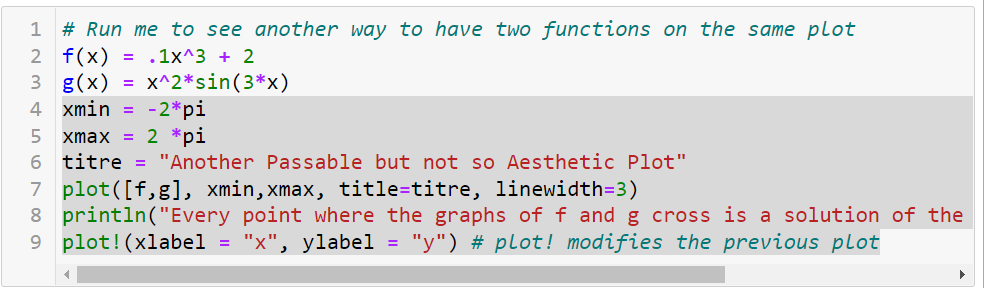
\includegraphics[width=0.9\columnwidth]{Chap02/MultiLineCommentingOut.png}}%
}

and then hit \texttt{Ctrl\,$/$} control-forward-slash (simultaneously) to comment out or un-comment multiple lines at a time. \\

\setlength{\fboxrule}{3pt}%
	\centerline{ \fbox{ 
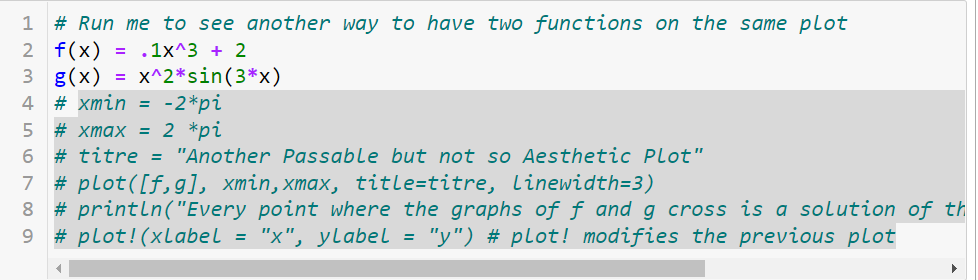
\includegraphics[width=0.9\columnwidth]{Chap02/MultiLineCommentingOut2.png}}%
}


\section{Applying Functions to Arrays via Broadcasting}

Julia has a special syntax for applying functions to individual elements of arrays. You need to add a ``dot'' after the function and before the argument to the function. It's best understood by doing it. 

\begin{lstlisting}[language=Julia,style=mystyle]
x = [0 pi/4 pi/2 3pi/4 pi 5pi/4]
\end{lstlisting}
\textbf{Output} 
\begin{verbatim}
1×6 Matrix{Float64}:
 0.0  0.785398  1.5708  2.35619  3.14159  3.92699
\end{verbatim}

\begin{lstlisting}[language=Julia,style=mystyle]
sin.(x)  # note the dot
\end{lstlisting}
\textbf{Output} 
\begin{verbatim}
1×6 Matrix{Float64}:
 0.0  0.707107  1.0  0.707107  1.22465e-16  -0.707107
\end{verbatim}

This also works with functions that you write yourself! It pretty awesome.

\begin{lstlisting}[language=Julia,style=mystyle]
f(x) = 1 + 2x + sin(x^2)
\end{lstlisting}
\textbf{Output} 
\begin{verbatim}
f (generic function with 1 method)
\end{verbatim}

\begin{lstlisting}[language=Julia,style=mystyle]
f.(x)  # note the dot
\end{lstlisting}
\textbf{Output} 
\begin{verbatim}
1×6 Matrix{Float64}:
 1.0  3.14927  4.76586  5.04438  6.85288  9.13678
\end{verbatim}

For an array,  $x = [x_1 ~~ x_2 ~~\ldots~~ x_n ]$, the returned value is $f.(x)=[f(x_1)~~  f(x_2)~~ \ldots ~~f(x_n)]$. This feature is called ``broadcasting''. If you leave out the ``dot'', this is what you get

\begin{lstlisting}[language=Julia,style=mystyle]
f(x)
\end{lstlisting}
\textbf{Output} 
\begin{verbatim}
DimensionMismatch("A has dimensions (1,6) but B has dimensions (1,6)")

Stacktrace:
  [1] gemm_wrapper!(C::Matrix{Float64}, tA::Char, tB::Char, A::Matrix{Float64},
  B::Matrix{Float64}, _add::LinearAlgebra.MulAddMul{true, true, Bool, Bool})
    @ LinearAlgebra /buildworker/worker/package_linux64/build/usr/share/julia/stdlib/
    v1.6/LinearAlgebra/src/matmul.jl:643
  [2] mul!
    @ /buildworker/worker/package_linux64/build/usr/share/julia/stdlib/v1.6/
    LinearAlgebra/src/matmul.jl:169 [inlined]
  [3] mul!
    @ /buildworker/worker/package_linux64/build/usr/share/julia/stdlib/v1.6/
    LinearAlgebra/src/matmul.jl:275 [inlined]
  [4] *
    @ /buildworker/worker/package_linux64/build/usr/share/julia/stdlib/v1.6/
    LinearAlgebra/src/matmul.jl:160 [inlined]
  [5] power_by_squaring(x_::Matrix{Float64}, p::Int64)
    @ Base ./intfuncs.jl:261
  [6] ^
    @ /buildworker/worker/package_linux64/build/usr/share/julia/stdlib/v1.6/
    LinearAlgebra/src/dense.jl:442 [inlined]
  [7] macro expansion
    @ ./none:0 [inlined]
  [8] literal_pow
    @ ./none:0 [inlined]
  [9] f(x::Matrix{Float64})
    @ Main ./In[8]:1
 [10] top-level scope
    @ In[10]:1
 [11] eval
    @ ./boot.jl:360 [inlined]
 [12] include_string(mapexpr::typeof(REPL.softscope), mod::Module, code::String,
 filename::String)
    @ Base ./loading.jl:1094

\end{verbatim}

You can also use the ``dot'' with addition or multiplication. Below, we add one to each entry of the array \texttt{x}. \\

\begin{lstlisting}[language=Julia,style=mystyle]
x .+ 1
\end{lstlisting}
\textbf{Output} 
\begin{verbatim}
1×6 Matrix{Float64}:
 1.0  1.7854  2.5708  3.35619  4.14159  4.92699
\end{verbatim}

The following code multiplies the entries of \texttt{x} times the corresponding entries in $y$,\\

\begin{lstlisting}[language=Julia,style=mystyle]
x = [1 2 3 4 5]
y = [5 4 3 2 1]
x.*y  # note the dot
\end{lstlisting}
\textbf{Output} 
\begin{verbatim}
1×5 Matrix{Int64}:
 5  8  9  8  5
\end{verbatim}

The same applies to squaring the entries of an array, such as \\

\begin{lstlisting}[language=Julia,style=mystyle]
x.^2  # note the dot
\end{lstlisting}
\textbf{Output} 
\begin{verbatim}
1×5 Matrix{Int64}:
 1  4  9  16  25
\end{verbatim}

The following applies the function $f(x)$ to each entry of \texttt{x} and then multiplies each entry of the resulting array times the corresponding entry in \texttt{y}.\\

\begin{lstlisting}[language=Julia,style=mystyle]
z=f.(x).*y  # we used two dots
\end{lstlisting}
\textbf{Output} 
\begin{verbatim}
1×5 Matrix{Float64}:
 19.2074  16.9728  22.2364  17.4242  10.8676
\end{verbatim}

The following applies the function $f(x)$ to each entry of \texttt{x}, then multiplies each entry of the resulting array times the corresponding entry in \texttt{y}, and finally adds 2 to each entry.\\

\begin{lstlisting}[language=Julia,style=mystyle]
z=f.(x).*y .+ 2  # we used three dots
\end{lstlisting}
\textbf{Output} 
\begin{verbatim}
1×5 Matrix{Float64}:
 21.2074  18.9728  24.2364  19.4242  12.8676
\end{verbatim}

\vspace*{.2cm}

\begin{center}
\fbox{ 
\textbf{
We note that $z = [z_1~~ z_2 ~~ \ldots~~ z_n]$, where for $1 \le i \le n$, the components of $z$ are given by $z_i = f(x_i)*y_i+ 2$.
}
}
\end{center}


% For emphasis, we note that $z = [z_1~~ z_2 ~~ \ldots~~ z_n]$, where for $1 \le i \le n$, the components of $z$ are given by $z_i = f(x_i)*y_i+ 2$.

\section{Debugging}

We created our first function in Chapter~\ref{sec:basicPlotting}. Here we'll show a common programming error that you might think is a bug.

\begin{lstlisting}[language=Julia,style=mystyle]
g=2 # set the variable g to a constant
\end{lstlisting}
\textbf{Output} 
\begin{verbatim}
2
\end{verbatim}

That's pretty simple! Now, imagine that you used the variable $g$ 15 cells back and have completely forgotten about it. You then want to create a function and call it $g$. 
\begin{lstlisting}[language=Julia,style=mystyle]
g(x) = 5x + 2
\end{lstlisting}
\textbf{Output} 
\begin{verbatim}
cannot define function g; it already has a value

Stacktrace:
 [1] top-level scope
   @ none:0
 [2] top-level scope
   @ In[4]:1
 [3] eval
   @ ./boot.jl:360 [inlined]
 [4] include_string(mapexpr::typeof(REPL.softscope), mod::Module, 
 code::String, filename::String)
   @ Base ./loading.jl:1094

\end{verbatim}

In the example, Cell [4] is the cell where we defined $g(x)$. There are two cures for this:
\begin{itemize}
    \item Clear your Kernel, \textbf{which will erase the variables in your Jupyter notebook without erasing your code}. You can then run the cell above again and it will work fine.

    \item Choose a different name for the function, which we illustrate below.
\end{itemize}
\begin{lstlisting}[language=Julia,style=mystyle]
g2(x) = 5x + 2
\end{lstlisting}
\textbf{Output} 
\begin{verbatim}
g2 (generic function with 1 method)
\end{verbatim}

\vspace*{.2cm}

\begin{tcolorbox}[title={\large \bf Debugging}]

    \begin{itemize}
        \item Taken From the Pro-tip page at Georgia Tech for a graduate-level course: \url{https://cse6040.gatech.edu/fa22/pro_tips.html}

        \item Debugging is an iterative process where you must trace the undesired behavior back to the root cause. Sometimes it's simple; other times it can be frustratingly complex.

        \item Identify what is wrong. This needs to be as precise as possible. If you don't understand the error in the traceback - Google it!. Check the syntax, parameters, and inputs of any function calls.

        \item Identify where the wrong thing got set. This will usually be an assignment or a function call.

        \item Rinse and repeat until you have found and corrected the root cause.
    \end{itemize}
\end{tcolorbox}

\chapter{Julia Lab 2: Vectors, Matrices, and Indexing}
\label{chap:Lab2}



\section*{Learning Objectives}

\begin{itemize}
\item  More ways to create vectors and matrices
\item  Indexing as a means to access the elements of vectors and matrices
\item Debugging, or finding and fixing errors in your code
\end{itemize}

\section*{Outcomes} 
\begin{itemize}
\item Vectors
\item Matrices
\begin{itemize}
\item \texttt{zeros}(n,m)
\item \texttt{ones}(n,m)
\item \texttt{using Random}
\item  \texttt{rand}(n,m) and \texttt{randn}(n,m)
    \end{itemize}
\item Adding columns or rows to matrices, concatenation
\item Indexing into row vectors (aka $1 \times n$ matrices in Julia ) and column vectors (aka simply a vector in Julia)
\item Indexing into matrices
\begin{itemize}
\item Extracting columns is easy
\item Extracting rows requires concentration
\item Extracting sub-matrices
\item Help command in Julia
    \end{itemize}
    \item Creating ``empty'' matrices via \texttt{Vector\{Float64\}(undef, n)} and  \texttt{Matrix\{Float64\}(undef, n, m)}, and 
    \item \texttt{B = copy(A)} and how that is different than \texttt{B=A}
    \item Creating an identity matrix in Julia is a bit odd.
\end{itemize}

\vspace*{1cm}

\textbf{Either download Lab2 from our Canvas site or open up a Jupyter notebook so that you can enter code as we go. It is suggested that you have line numbering toggled on.}  

\newpage

At the end of Lab 1, we saw how to create (small) row vectors, columns vectors and $n \times m$ matrices. You may want to review that material before starting here.\\

\section{Friendly Checks}

In your lab assignments, Julia HWs, and Projects, we are inserting here and there a means to detect errors in your code before you get too deep into the assignments. \textcolor{red}{\bf Mostly, we are not checking that you are correct, we are instead checking that you are not obviously wrong.} In mathematical language, we are checking ``necessary conditions'' but not ``sufficient conditions'' for you to be correct. In simple terms, you can pass our tests, and still be wrong. You will just not be wrong in a way that we anticipated, which is kind of a bummer for you. 


\begin{rem} We have messed up in the past by updating the numbers in a problem and failing to update the associated tests! If you and your classmates are all failing a test, let us know and we'll double check our test. In the end, we are trying to decrease your frustration and uncertainty. Sometimes, we add to it! C'est la vie !
\end{rem}

Here is an example of how the tests work.
\begin{lstlisting}[language=Julia,style=mystyle]
# Warm up work for you: # Create a column vector (called almost_zero_vec) 
# that has 4 entries: the 2nd entry is -2.5, and others are zeros
# 
almost_zero_vec = NaN    #Replace NaN with your answer
\end{lstlisting}
\textbf{Output} 
\begin{verbatim}
NaN
\end{verbatim}


Here is the solution:
\begin{lstlisting}[language=Julia,style=mystyle]
# Warm up work for you: # Create a column vector (called almost_zero_vec) 
# that has 4 entries: the 2nd entry is -2.5, and others are zeros
# 
almost_zero_vec = [0, -2.5, 0, 0]    #Replace NaN with your answer
\end{lstlisting}
\textbf{Output} 
\begin{verbatim}
4-element Vector{Float64}:
  0.0
 -2.5
  0.0
  0.0
\end{verbatim}

Here is an example test, \textbf{designed to not give away the answer and yet, try to let you know if you are wrong}:

\begin{lstlisting}[language=Julia,style=mystyle]
# friendly check
test1 = almost_zero_vec'*almost_zero_vec
ind = [1 3 4]
test2 = sum(abs.(almost_zero_vec[ind]))
test3 = length(almost_zero_vec)

is_it_correct_check1 = (test1 == 6.25) ? "Yes" : "No" 
is_it_correct_check2 = (test2 == 0.0) ? "Yes" : "No"
is_it_correct_check3 = (test3 == 4) ? "Yes" : "No"

@show is_it_correct_check1;  
@show is_it_correct_check2; 
@show is_it_correct_check3;  
\end{lstlisting}
\textbf{Output} 
\begin{verbatim}
is_it_correct_check1 = "Yes"
is_it_correct_check2 = "Yes"
is_it_correct_check3 = "Yes"
\end{verbatim}

In this case, you're good to go. Suppose you had instead posed the solution as 

\begin{lstlisting}[language=Julia,style=mystyle]
# Warm up work for you: # Create a column vector (called almost_zero_vec) 
# that has 5- entries: the 2nd entry is -2.5, and others are zeros
# 
almost_zero_vec = [0, 2.5, 0, 0, 0]    #Replace NaN with your answer
\end{lstlisting}
\textbf{Output} 
\begin{verbatim}
5-element Vector{Float64}:
 0.0
 2.5
 0.0
 0.0
 0.0
\end{verbatim}

Then the friendly test let's you know that something is wrong via the line \texttt{is\_it\_correct\_check3 = "No"}. \textbf{That you failed \texttt{test3} is not meant to be particularly helpful to your debugging process.} You can ignore that part. 
\begin{lstlisting}[language=Julia,style=mystyle]
@show is_it_correct_check3;  
\end{lstlisting}
\textbf{Output} 
\begin{verbatim}
is_it_correct_check1 = "Yes"
is_it_correct_check2 = "Yes"
is_it_correct_check3 = "No"
\end{verbatim}
\textcolor{red}{\bf Most of our tests do not specify the nature of your mistake.} You need to find it yourself. Our goal is simply to prevent you from compounding errors as you proceed with an assignment. You may be able to study our error-checking code to see, as in this case, we were checking the \texttt{length} of the vector (a command we have not yet taught you), but normally we try to hide what we are checking. \\

Below is a wrong answer that passes our test because we are not checking the sign of the non-zero number. We just assume you will get that part correct. 

\begin{lstlisting}[language=Julia,style=mystyle]
# Warm up work for you: # Create a column vector (called almost_zero_vec) 
# that has 4 entries: the 2nd entry is -2.5, and others are zeros
# 
almost_zero_vec = [0, 2.5, 0, 0]    #Replace NaN with your answer
\end{lstlisting}
\textbf{Output} 
\begin{verbatim}
4-element Vector{Float64}:
  0.0
  2.5
  0.0
  0.0
\end{verbatim}

The output of the test code is 
\begin{verbatim}
is_it_correct_check1 = "Yes"
is_it_correct_check2 = "Yes"
is_it_correct_check3 = "Yes"
\end{verbatim}

\textcolor{red}{\bf From the Friendly check, it looks like you are good to go, even though you got the sign wrong.} On the other hand, you had the right number of elements, the magnitude of the second value was correct, and you had the zero elements in the correct locations. We checked for a lot of things, but not everything. In the pilot offering of ROB 101, there were no friendly checks at all! 

\section{New Ways to Create Matrices}

\subsection{Using Built-in Functions}

We'll quickly illustrate the following methods for creating matrices. The \texttt{rand} command is very useful for creating examples that have hundreds of variables (for later in the course).
\begin{itemize}
\item \texttt{zeros}(n,m)
\item \texttt{ones}(n,m)
\item \texttt{using Random}
\item  \texttt{rand}(n,m) (uniform) and with an extra ``n'' \texttt{randn}(n,m) (normal, aka Gaussian or Bell Curve)
    \end{itemize}


\begin{lstlisting}[language=Julia,style=mystyle]
# Creates a matrix of zeros with n-rows and m-columns
A = zeros(3,5)
\end{lstlisting}
\textbf{Output} 
\begin{verbatim}
3×5 Matrix{Float64}:
 0.0  0.0  0.0  0.0  0.0
 0.0  0.0  0.0  0.0  0.0
 0.0  0.0  0.0  0.0  0.0
\end{verbatim}


\begin{lstlisting}[language=Julia,style=mystyle]
# Creates a matrix of ones with n-rows and m-columns
B = ones(5,3)
\end{lstlisting}
\textbf{Output} 
\begin{verbatim}
5×3 Matrix{Float64}:
 1.0  1.0  1.0
 1.0  1.0  1.0
 1.0  1.0  1.0
 1.0  1.0  1.0
 1.0  1.0  1.0
\end{verbatim}

\begin{lstlisting}[language=Julia,style=mystyle]
# Install the package Random
using Random
\end{lstlisting}
\textbf{Output} 
\begin{verbatim}
(none)
\end{verbatim}

The command \texttt{rand}(n) or \texttt{rand}(n,m) produces numbers that are ``uniformly distributed between zero and one''. This roughly means that each $x \in [0, 1]$ is equally likely; a more precise statement would be that, for all $0\le a < b \le 1$, the probability that $x \in [a, b]$ is equal to $b-a$. The related command \texttt{randn}(n) or \texttt{randn}(n,m) produces numbers that are ``normally distributed between minus infinity and plus infinity''. This means that the random number comes from a Bell curve. 

\begin{lstlisting}[language=Julia,style=mystyle]
# Run me
Random.seed!(4321) # Set the seed so that each of you get the same results. 
@show myVector = rand(9) # column vector
myMatrix = rand(3,4)  # 3 x 4 matrix with random entries in [0,1]
\end{lstlisting}
\textbf{Output} 
\begin{verbatim}
myVector = rand(9) = [0.1619496289112512, 0.1385032717390522, 0.6355055732000539,
0.36326986232801595, 0.3700559311804976, 0.8332539255123794, 0.6910169607353331,
0.08205602210008567, 0.6441883306325207]

3×4 Matrix{Float64}:
 0.873045  0.413895  0.0578154  0.55376
 0.705639  0.492289  0.914811   0.544223
 0.528017  0.24885   0.917523   0.478742
\end{verbatim}


\begin{lstlisting}[language=Julia,style=mystyle]
# Run me
Random.seed!(4321) # Set the seed so that each of you get the same results. 
myMatrix = randn(6,5)  # 6 x 5 matrix with random entries in (-inf, inf)
\end{lstlisting}
\textbf{Output} 
\begin{verbatim}
6×5 Matrix{Float64}:
 -0.229071  -0.991273  -0.850184   -1.06297     0.609128
  0.321924  -0.158205   0.592798   -0.509626   -0.547334
  0.74283    1.02869   -0.358643    0.673963    0.24726
  0.948465  -1.94117   -0.0688075   0.317936   -0.860824
 -0.540755  -1.00753    1.51188    -1.13022     1.45335
 -1.95979    0.825056  -0.718068   -0.0391889   0.453098
\end{verbatim}

\begin{lstlisting}[language=Julia,style=mystyle]
# Run me
# if we do not set the seed, each time we get a new set of random numbers. 
myMatrix = randn(6,5)  # 6 x 5 matrix with random entries in (-inf, inf)
\end{lstlisting}
\textbf{Output} 
\begin{verbatim}
6×5 Matrix{Float64}:
  0.498376   0.411742  -0.753106  -0.984998   0.53562
 -0.670348  -0.826093  -0.219619  -0.582682   0.151646
 -0.52135    0.680463   0.885311  -0.703102   1.64057
 -0.71363   -0.322208  -0.991709  -1.44334   -1.41471
  0.249046   0.373825  -1.04189   -0.254509  -0.0348657
  0.851102  -0.044526  -1.34575    2.70248    0.666966
\end{verbatim}



We'll use the ability to generate random matrices of arbitrary size when we start testing our own algorithms. Let's try \texttt{A = randn(100,100)}. Julia cannot printout all of its entries. Julia is showing here the first three columns and last three columns, of the first 13 rows and the last 12 rows. 



\begin{lstlisting}[language=Julia,style=mystyle]
# Run me
A = randn(100,100)
\end{lstlisting}
\textbf{Output} 
\begin{verbatim}
100×100 Matrix{Float64}:
 -1.21507     1.51014     -0.358913  ... 0.202398    0.92658     0.300415
 -0.0293227  -0.643004     0.941623      0.326798   -0.847375    0.174174
  1.20972    -0.745284    -1.57119       1.13692    -2.35792    -0.191441
 -0.36017    -0.400969     0.398202     -0.194262   -0.785111   -0.764176
  0.243962    0.102421    -1.74552       0.0195486  -0.475647    1.23968
 -0.586099   -0.481138    -0.396337  ... 2.16696     0.145727    0.348194
  0.810478   -1.41851      0.661778     -0.110213    0.397295    0.908824
 -0.173821   -0.0334777    0.593349      1.00495    -1.38393    -1.6448
 -1.13339    -0.911688     1.52026      -0.293288    0.612828    0.45864
  0.493715   -2.1743      -1.14563       1.00688    -1.27257    -0.0470864
  1.03548     1.01407     -0.586865  ...-1.33328     0.683025    0.215578
 -0.208806    0.89081      1.14522       1.05247     0.55675    -0.0393328
 -0.730545   -0.51702      0.642981      0.429845   -0.869449    0.75665
    .                                .
    .                                .
    .                                .
 -0.421939   -0.66485     -1.33336      -1.06668     0.0644415   0.0635774
 -1.18934    -0.465795     0.461657      0.247114   -1.71652    -1.9573
 -0.129762    0.434988     0.23351   ...-0.875235   -0.963982   -0.247793
  1.2493      0.646449     0.236439     -0.861302   -0.764389    0.858528
 -0.516579    0.0443446   -1.08403      -1.23918    -1.24305    -0.386032
 -0.916162   -0.0758758   -0.421691      1.52287     0.527025    1.24463
 -0.684109   -0.107738    -0.461977     -0.110118    1.00922     0.489418
 -1.11484    -0.38536     -0.631     ... 1.24931    -0.290083    1.79908
 -0.0738447   1.76986      1.21057       0.575938   -0.275458    0.324595
  0.0713201   0.190427    -1.85452       1.33801    -0.0978082   0.34016
  0.238514    1.22612      0.177986     -1.08624     1.82018    -0.47512
  0.249298    0.00947162  -1.33509      -0.728613   -0.992987    0.0453849
  
\end{verbatim}

\subsection{Concatenation or Adding Columns and Rows to Matrices}

Another way to build a matrix is by concatenating columns or rows. We illustrate that now.\\

Suppose that $v_1, \ldots, v_4$ are row vectors (what Julia calls a $1 \times n$ matrix). Then we can use them as the rows of a matrix, as in 
$$ M = \begin{bmatrix}
v_1 \\
v_2 \\
v_3\\
v_4    
\end{bmatrix}
$$

Similarly, suppose that $v_1, \ldots, v_4$ are column vectors (what Julia calls a vector). Then we can use them as the columns of a matrix, as in 
$$ M = \begin{bmatrix}
v_1 & v_2 & v_3 & v_4    
\end{bmatrix}
$$

\begin{lstlisting}[language=Julia,style=mystyle]
vRow1 = [1 2 3]
vRow2 = [4 5 6]
vRow3 = [7 8 9]
vRow4 = [10 11 12]
#
# We will concatenate the row vectors to form a 4 x 3 matrix
#
M = [vRow1; vRow2; vRow3; vRow4] # separated by semicolons
\end{lstlisting}
\textbf{Output} 
\begin{verbatim}
4×3 Matrix{Int64}:
  1   2   3
  4   5   6
  7   8   9
 10  11  12
\end{verbatim}

\begin{lstlisting}[language=Julia,style=mystyle]
vCol1 = [1, 2, 3]
vCol2 = [4, 5, 6]
vCol3 = [7, 8, 9]
vCol4 = [10, 11, 12]
#
# We will concatenate the column vectors to form a 3 x 4 matrix
#
M = [vCol1 vCol2 vCol3 vCol4]  # separated by spaces
\end{lstlisting}
\textbf{Output} 
\begin{verbatim}
3×4 Matrix{Int64}:
 1  4  7  10
 2  5  8  11
 3  6  9  12
\end{verbatim}

We can even build matrices from other matrices, as long as they are \textbf{size compatible}. We illustrate. Suppose that $A_{11}$ is $n_1 \times m_1$ and $A_{12}$ is $n_1 \times m_2$, where both $A_{11}$ and $A_{12}$ have the same number of rows. Then we can form 
$$ M = \begin{bmatrix}
A_{11} & A_{12}   
\end{bmatrix}.
$$
$M$ now has $m_1 + m_2$ columns. Hence, if $B$ is $n_2 \times (m_1 + m_2)$, then it has the same number of columns as $M$ and thus we can add $B$ to $M$ as additional rows, like this,
$$ N = \begin{bmatrix}
M \\ B 
\end{bmatrix} = \left[ \begin{array}{c} A_{11} ~~~~ A_{12} \\ B  \end{array} \right].
$$
we illustrate this now.

\begin{lstlisting}[language=Julia,style=mystyle]
A11 = [1 2; 3 4]
A12 = [5; 6]
M = [A11 A12]
display(M)

B = [7 8 9; 10 11 12]
display(B)

N = [M;B] # Build the matrix piece by piece
display(N) 

N2 = [A11 A12; B] # Build the matrix all at once. Both are fine.
\end{lstlisting}
\textbf{Output} 
\begin{verbatim}
2×3 Matrix{Int64}:
 1  2  5
 3  4  6
 
2×3 Matrix{Int64}:
  7   8   9
 10  11  12
 
4×3 Matrix{Int64}:
  1   2   5
  3   4   6
  7   8   9
 10  11  12
 
4×3 Matrix{Int64}:
  1   2   5
  3   4   6
  7   8   9
 10  11  12
\end{verbatim}

\begin{lstlisting}[language=Julia,style=mystyle]
# With practice, you do this
A11 = [1 2; 3 4]
A12 = [5; 6]
B = [7 8 9; 10 11 12]

C = [A11 A12; B] 
\end{lstlisting}
\textbf{Output} 
\begin{verbatim}
2×3 Matrix{Int64}:
 1  2  5
 3  4  6
 
1×3 Matrix{Int64}:
 7  8  9
 
3×3 Matrix{Int64}:
 1  2  5
 3  4  6
 7  8  9
\end{verbatim}

If $A_{11}$, $A_{12}$, $A_{21}$, and $A_{22}$ are size compatible matrices, we can do this
$M = \begin{bmatrix}
    A_{11} & A_{12} \\ A_{21} & A_{22}
\end{bmatrix}.$

What do the sizes have to be?  
\begin{itemize}
    \item $A_{11}$ and $A_{12}$ must have the same number of rows, so that we can form $\left[A_{11} ~~~ A_{12} \right]$.
    \item $A_{21}$ and $A_{22}$ must have the same number of rows, which can be different from $A_{11}$ and $A_{12}$. This allows the formation of $\left[ A_{21} ~~~ A_{22} \right]$.
    \item $\left[A_{11} ~~~ A_{12} \right]$ and $\left[ A_{21} ~~~ A_{22} \right]$ must have the same number of columns. 
    \item In other words, if $A_{ij}$ is $n_{ij} \times m_{ij}$, then we need
    \begin{itemize}
        \item[*] $n_{11} = n_{12}$ (rows match)
        \item[*] $n_{21} = n_{22}$ (rows match)
        \item[*] $m_{11} +m_{12} = m_{21} +m_{22}$ (column sums match)
    \end{itemize}
\end{itemize}

\begin{lstlisting}[language=Julia,style=mystyle]
A11 = [1 2; 3 4]
A12 = [5; 6]
A21 = [7;8]
A22 = [9 10; 11 12]

M = [A11 A12; A21 A22] 
\end{lstlisting}
\textbf{Output} 
\begin{verbatim}
4×3 Matrix{Int64}:
 1   2   5
 3   4   6
 7   9  10
 8  11  12
\end{verbatim}


\section{Indexing or Slicing Vectors}

\begin{rem}
\textcolor{red}{\bf Julia uses **1-based indexing** which means that the index starts at 1 and not 0.} Be aware that 0-based indexing is used in some other programming languages, such as C++. If you are familiar with MATLAB, it uses 1-based indexing.
\end{rem}


\begin{lstlisting}[language=Julia,style=mystyle]
# Run me to define some vectors and matrices
@show row_vec = [1 3 5 7 9] # spaces make me a row vector
almost_zero_vec=[0; 0; -pi; 0; 0; 0; 0] # the semicolons (commas also work) 
                                    # make me a column vector 
\end{lstlisting}
\textbf{Output} 
\begin{verbatim}
row_vec = [1 3 5 7 9] = [1 3 5 7 9]

7-element Vector{Float64}:
  0.0
  0.0
 -3.141592653589793
  0.0
  0.0
  0.0
  0.0
\end{verbatim}


\begin{lstlisting}[language=Julia,style=mystyle]
# Select the 1st entry from row_vector
num = row_vec[1]
#= Can you tell that the type of num is Int64? 
If you are unsure, uncomment and run the next command
=#
# typeof(num)
\end{lstlisting}
\textbf{Output} 
\begin{verbatim}
1
\end{verbatim}

\begin{lstlisting}[language=Julia,style=mystyle]
# Select the non-zero number from almost_zero_vec
num = almost_zero_vec[3]
# Note: because a vector has only one dimension, 
# only one index is needed and it corresponds to 
# the location where the number is stored
\end{lstlisting}
\textbf{Output} 
\begin{verbatim}
-3.141592653589793
\end{verbatim}

\textcolor{red}{\bf You can select multiple entries at one time.}

\begin{lstlisting}[language=Julia,style=mystyle]
# Select the first, second, and fourth entries of the 
# vector row_vec and return them as a row vector
#
ind = [1 2 4] # note the use of spaces instead of commas 
#             or semicolons so as to return a row vector.
result = row_vec[ind]
\end{lstlisting}
\textbf{Output} 
\begin{verbatim}
1×3 Matrix{Int64}:
 1  3  7
\end{verbatim}


\begin{lstlisting}[language=Julia,style=mystyle]
# You can also do it like this, but it's kind of ugly
result = row_vec[[1 2 4]]
\end{lstlisting}
\textbf{Output} 
\begin{verbatim}
1×3 Matrix{Int64}:
 1  3  7
\end{verbatim}


\begin{lstlisting}[language=Julia,style=mystyle]
# Select the first, second, and fourth entries of the 
# vector row_vec and return then as a column vector
#
ind = [1, 2, 4] # note the use of commas (semicolons also work) 
#                 so as to return a column vector.
result = row_vec[ind]
\end{lstlisting}
\textbf{Output} 
\begin{verbatim}
3-element Vector{Int64}:
 1
 3
 7
\end{verbatim}

\section{Indexing or Slicing Matrices}

\begin{rem}
We recall once again that Julia uses \textbf{**1-based indexing**} which means that the index starts at 1 and not 0. Be aware that 0-based indexing is used in some other programming languages, such as C++. If you are familiar with MATLAB, it uses 1-based indexing.
\end{rem}

\begin{lstlisting}[language=Julia,style=mystyle]
# Run me to define a matrix with random numbers
#
using Random # Using an external package called Random 
Random.seed!(1234) # Set the seed so that each of you gets the same results. 
rand_matrix = rand(4, 6)
\end{lstlisting}
\textbf{Output} 
\begin{verbatim}
4×6 Matrix{Float64}:
 0.590845  0.794026  0.246837   0.066423  0.276021   0.950498
 0.766797  0.854147  0.579672   0.956753  0.651664   0.96467
 0.566237  0.200586  0.648882   0.646691  0.0566425  0.945775
 0.460085  0.298614  0.0109059  0.112486  0.842714   0.789904
\end{verbatim}



\begin{lstlisting}[language=Julia,style=mystyle]
# Select the entry in the 2nd row and 3rd column of rand_matrix
#
myNum = rand_matrix[2, 3]
#
# Note: 2 is the index for the row, and 3 is the index for the column
#
# Can you tell that the type of myNum is Float64? 
# If you are unsure, uncomment and run the next command
# typeof(myNum)
\end{lstlisting}
\textbf{Output} 
\begin{verbatim}
0.5796722333690416
\end{verbatim}

\begin{lstlisting}[language=Julia,style=mystyle]
# Select the entire 4th column of rand_matrix
#
myVect = rand_matrix[:, 4]
#
# Note: when we want to select the whole column, 
# we use `:` as the index for row, and vice versa. 
# The symbol ":" stands for "all entries" 
\end{lstlisting}
\textbf{Output} 
\begin{verbatim}
4-element Vector{Float64}:
 0.06642303695533736
 0.9567533636029237
 0.646690981531646
 0.11248587118714015
\end{verbatim}

\begin{rem}
Selecting a row of a matrix is trickier than selecting a column. Pay attention here. \textcolor{red}{\bf This is very different than MATLAB.}
\end{rem}

\begin{lstlisting}[language=Julia,style=mystyle]
# Select the 2nd row of rand_matrix
#
myVect = rand_matrix[2:2, :]  # note the use of "2:2" instead of simply "2"
\end{lstlisting}
\textbf{Output} 
\begin{verbatim}
1×6 Matrix{Float64}:
 0.766797  0.854147  0.579672  0.956753  0.651664  0.96467
\end{verbatim}

\begin{rem}
\textcolor{red}{\bf Pay attention here. This is very different than MATLAB.} Julia hates row vectors so much that it calls a row vector a $1 \times n$ \texttt{Matrix}. Every chance it gets, Julia creates a column vector and then calls it an $n$-element \texttt{Vector}. You need to be aware of this peculiarity of the language. Forgetting it will lead to frustration and heartbreak! 
\end{rem}

\begin{lstlisting}[language=Julia,style=mystyle]
# If you only place a "2" instead of "2:2" you get a column vector
#
myVect = rand_matrix[2, :]
\end{lstlisting}
\textbf{Output} 
\begin{verbatim}
6-element Vector{Float64}:
 0.7667970365022592
 0.8541465903790502
 0.5796722333690416
 0.9567533636029237
 0.6516642063795697
 0.9646697763820897
\end{verbatim}


\begin{lstlisting}[language=Julia,style=mystyle]
# What if you use the m:m trick on a column?
#
myVect = rand_matrix[:, 4:4]
#
# You get a 4 x 1 Matrix. While this is not a Vector in Julia, 
# for most uses, it is perfectly fine.
\end{lstlisting}
\textbf{Output} 
\begin{verbatim}
4×1 Matrix{Float64}:
 0.06642303695533736
 0.9567533636029237
 0.646690981531646
 0.11248587118714015
\end{verbatim}

\section{More Advanced Remarks on Indexing}

We'll use the matrix \texttt{rand\_matrix} to show how to select ``sub-matrices'' from it.

\begin{lstlisting}[language=Julia,style=mystyle]
# Run me
rand_matrix
\end{lstlisting}
\textbf{Output} 
\begin{verbatim}
4×6 Matrix{Float64}:
 0.590845  0.794026  0.246837   0.066423  0.276021   0.950498
 0.766797  0.854147  0.579672   0.956753  0.651664   0.96467
 0.566237  0.200586  0.648882   0.646691  0.0566425  0.945775
 0.460085  0.298614  0.0109059  0.112486  0.842714   0.789904
\end{verbatim}

\vspace*{.2cm}

\textcolor{blue}{\bf We will now select out the rows in red,}
\begin{equation}
\left[
\begin{array}{cccccc}
0.5908 & 0.7940 & 0.2468 & 0.0664 & 0.2760 & 0.9505 \\
\RED 0.7668 & \RED 0.8541 &  \RED 0.5797 & \RED 0.9568 & \RED 0.6517 & \RED 0.9647 \\
0.5662 & 0.2006 &  0.6489 &  0.6467 & 0.0566 & 0.9458 \\
\RED 0.4601 & \RED 0.2986 & \RED 0.0109 & \RED 0.1125 & \RED 0.8427 & \RED 0.7899 \\
\end{array}
\right]
\end{equation}



\begin{lstlisting}[language=Julia,style=mystyle]
indRow = [2, 4]             # Note that we wanted all the columns, 
mySlice=rand_matrix[indRow,:]  # so we use the colon : to do that
\end{lstlisting}
\textbf{Output} 
\begin{verbatim}
2x6 Matrix{Float64}:
 0.766797  0.854147  0.579672   0.956753  0.651664  0.96467
 0.460085  0.298614  0.0109059  0.112486  0.842714  0.789904
\end{verbatim}

\textcolor{blue}{\bf We will now select out the columns in red,}
\begin{equation}
\left[
\begin{array}{cccccc}
0.5908 & 0.7940 & \RED 0.2468 & 0.0664 & \RED 0.2760 & \RED 0.9505 \\
0.7668 & 0.8541 &  \RED 0.5797 &  0.9568 & \RED 0.6517 & \RED 0.9647 \\
0.5662 & 0.2006 &  \RED 0.6489 &  0.6467 & \RED 0.0566 & \RED 0.9458 \\
0.4601 & 0.2986 & \RED 0.0109 & 0.1125 & \RED 0.8427 & \RED 0.7899 \\
\end{array}
\right]
\end{equation}



\begin{lstlisting}[language=Julia,style=mystyle]
indCol = [3, 5, 6]          # Note that we wanted all the rows, 
mySlice=rand_matrix[:,indCol]  # so we use the colon : to do that
\end{lstlisting}
\textbf{Output} 
\begin{verbatim}
4x3 Matrix{Float64}:
 0.246837   0.276021   0.950498
 0.579672   0.651664   0.96467
 0.648882   0.0566425  0.945775
 0.0109059  0.842714   0.789904
\end{verbatim}


\textcolor{blue}{\bf We will now select out the entries in red,}
\begin{equation}
\left[
\begin{array}{cccccc}
0.5908 & 0.7940 & 0.2468 & 0.0664 & 0.2760 & 0.9505 \\
0.7668 & 0.8541 & \RED 0.5797 & \RED 0.9568 & 0.6517 & 0.9647 \\
0.5662 & 0.2006 & \RED 0.6489 & \RED 0.6467 & 0.0566 & 0.9458 \\
0.4601 & 0.2986 & 0.0109 & 0.1125 & 0.8427 & 0.7899 \\
\end{array}
\right]
\end{equation}


\begin{lstlisting}[language=Julia,style=mystyle]
# Select rows 2 and 3 of columns 3 and 4
indRow = [2, 3] # Yes, commas are used. Try it without the commas here
indCol = [3, 4]
mySlice=rand_matrix[indRow,indCol]
\end{lstlisting}
\textbf{Output} 
\begin{verbatim}
2×2 Matrix{Float64}:
 0.579672  0.956753
 0.648882  0.646691
\end{verbatim}

\textcolor{blue}{\bf We will next select out the entries in red,}
\begin{equation}
\left[
\begin{array}{cccccc}
\RED 0.5908 & 0.7940 & 0.2468 & 0.0664 & 0.2760 & \RED 0.9505 \\
\RED 0.7668 & 0.8541 &  0.5797 &  0.9568 & 0.6517 &\RED  0.9647 \\
0.5662 & 0.2006 &  0.6489 &  0.6467 & 0.0566 & 0.9458 \\
\RED 0.4601 & 0.2986 & 0.0109 & 0.1125 & 0.8427 & \RED 0.7899 \\
\end{array}
\right]
\end{equation}

\begin{lstlisting}[language=Julia,style=mystyle]
# Select rows 1,2, and 4 of columns 1 and 6
indRow = [1, 2, 4] # Yes, commas are used. Try it without the commas here
indCol = [1, 6]
mySlice=rand_matrix[indRow,indCol]
\end{lstlisting}
\textbf{Output} 
\begin{verbatim}
3×2 Matrix{Float64}:
 0.590845  0.950498
 0.766797  0.96467
 0.460085  0.789904
\end{verbatim}

\textcolor{blue}{\bf We will select out the entries in red,}
\begin{equation}
\left[
\begin{array}{cccccc}
0.5908 & 0.7940 & 0.2468 & 0.0664 & 0.2760 & 0.9505 \\
0.7668 & 0.8541 & \RED 0.5797 & \RED 0.9568 & \RED0.6517 & \RED0.9647 \\
0.5662 & 0.2006 & \RED 0.6489 & \RED 0.6467 & \RED0.0566 & \RED0.9458 \\
0.4601 & 0.2986 & 0.0109 & 0.1125 & 0.8427 & 0.7899 \\
\end{array}
\right]
\end{equation}

\begin{lstlisting}[language=Julia,style=mystyle]
# Select from column 3 to the end of rows 2 and 3
indRow = [2, 3] # Yes, commas are used. Try it without the commas here
mySlice=rand_matrix[indRow,3:end] # note 3:end is the same as 3:6
\end{lstlisting}
\textbf{Output} 
\begin{verbatim}
2×4 Matrix{Float64}:
 0.579672  0.956753  0.651664   0.96467
 0.648882  0.646691  0.0566425  0.945775
\end{verbatim}

\textcolor{blue}{\bf Here is another way to do the same thing,}
\begin{lstlisting}[language=Julia,style=mystyle]
# Select from column 3 to the end of rows 2 and 3
indRow = [2, 3] # Yes, commas are used. Try it without the commas here
indCol = collect(3:6) # look up the command ``collect''
@show indCol
mySlice=rand_matrix[indRow,indCol]] 
\end{lstlisting}
\textbf{Output} 
\begin{verbatim}
indCol = [3, 4, 5, 6]

2×4 Matrix{Float64}:
 0.579672  0.956753  0.651664   0.96467
 0.648882  0.646691  0.0566425  0.945775
\end{verbatim}

\begin{rem}
To get help on a function in Julia, use a question mark, followed by a space, followed by the name of the function. We illustrate here for the function \texttt{collect}
\end{rem}

\begin{lstlisting}[language=Julia,style=mystyle]
? collect
\end{lstlisting}
\textbf{Output} 
\begin{verbatim}
search: collect

collect(element_type, collection)
Return an Array with the given element type of all items in a collection or iterable. 
The result has the same shape and number of dimensions as collection.

Examples
julia> collect(Float64, 1:2:5)
3-element Vector{Float64}:
 1.0
 3.0
 5.0
collect(collection)
Return an Array of all items in a collection or iterator. For dictionaries, returns
Pair{KeyType, ValType}. If the argument is array-like or is an iterator with the
[HasShape](@ref IteratorSize) trait, the result will have the same shape and number of
dimensions as the argument.

Examples
julia> collect(1:2:13)
7-element Vector{Int64}:
  1
  3
  5
  7
  9
 11
 13
\end{verbatim}
\begin{rem}
At least in the ROB 101 version of Julia, any call to a help function must be the only thing in the cell. Even inserting a comment breaks the help command.
\end{rem}

\begin{lstlisting}[language=Julia,style=mystyle]
# see what happens when you lead with a comment
? collect
\end{lstlisting}
\textbf{Output} 
\begin{verbatim}
syntax: invalid identifier name "?"

Stacktrace:
 [1] top-level scope
   @ In[11]:2
 [2] eval
   @ ./boot.jl:360 [inlined]
 [3] include_string(mapexpr::typeof(REPL.softscope), mod::Module, code::String,
 filename::String)
   @ Base ./loading.jl:1094
\end{verbatim}



\section{Advanced Methods for Creating Vectors and Matrices}
\label{sec:Chap2:AdvancedMethodsCreatingMatrices}

We'll illustrate the commands \texttt{Vector\{Float64\}(undef, n)} and  \texttt{Matrix\{Float64\}(undef, n, m)} for creating vectors and matrices. They allow you to define a vector or matrix of a specified size without specifying its entries. We'll also illustrate the \texttt{copy} command for creating a copy of a matrix and how to make an identity matrix.
\begin{itemize}
    \item \texttt{Vector\{Float64\}(undef, n)}
    \item \texttt{Matrix\{Float64\}(undef, n, m)}
    \item where \texttt{undef} is a Julia keyword to create a value that is ``undefined'', and
    \item $n$ defines the number of rows and $m$ the number of columns. 
    \item \texttt{B=copy(A)} 
    \item How to create an identify matrix \texttt{Id = zeros(n,n) + I}.
\end{itemize}

Notice that when Julia creates a vector or matrix using the \texttt{Vector\{Float64\}(undef, n)} and  \texttt{Matrix\{Float64\}(undef, n, m)}  commands, it fills its entries with tiny numbers. How tiny? Well, the age of the universe in seconds is approximately 4.2$\times 10^{16}$. Hence, each second is approximately $2.3\times 10^{-17}$-th of the age of the universe. Let's say a typical ant that shows up in your home is half a centimeter long. Then that ant is $1.25\times 10^{-10}$ of the circumference of the earth (which is approximately 40,000 km). Julia is using numbers with $10^{-310}.$ I hope these comparisons were both helpful and interesting! \\

\begin{lstlisting}[language=Julia,style=mystyle]
Vector{Float64}(undef, 5)
\end{lstlisting}
\textbf{Output} 
\begin{verbatim}
5-element Vector{Float64}:
 0.0
 5.0e-324
 6.9094653095626e-310
 1.0e-323
 5.0e-324
\end{verbatim}

\begin{lstlisting}[language=Julia,style=mystyle]
Matrix{Float64}(undef, 3, 4)
\end{lstlisting}
\textbf{Output} 
\begin{verbatim}
3×4 Matrix{Float64}:
 6.90947e-310  6.90947e-310  6.90947e-310  6.90947e-310
 6.90947e-310  6.90947e-310  6.90947e-310  6.9094e-310
 6.90947e-310  6.90947e-310  6.90947e-310  6.90947e-310
\end{verbatim}

\textbf{The Copy command is more important than you might think.} The command \texttt{C=A} creates the matrix \texttt{C} and sets all of its entries equal to those of \texttt{A}. So far so good. It also links \texttt{C} to the matrix \texttt{A} so that any changes made to \texttt{C} are also made in \texttt{A} and vice versa. The command \texttt{B=copy(A)} creates an \textbf{independent} copy of $A$. Changes made in \texttt{B} do not show up in \texttt{A} and vice versa. Study the following examples and create a few of your own:\\

\begin{lstlisting}[language=Julia,style=mystyle]
A=[1.9 2.0; 3.0 4.0]
C=A
\end{lstlisting}
\textbf{Output} 
\begin{verbatim}
2×2 Matrix{Float64}:
 1.0  2.0
 3.0  4.0
\end{verbatim}

\begin{lstlisting}[language=Julia,style=mystyle]
C[1,2]=pi
C
\end{lstlisting}
\textbf{Output} 
\begin{verbatim}
2×2 Matrix{Float64}:
 1.0  3.14159
 3.0  4.0
\end{verbatim}

Now, look at the matrix $A$. \\
\begin{lstlisting}[language=Julia,style=mystyle]
A
\end{lstlisting}
\textbf{Output} 
\begin{verbatim}
2×2 Matrix{Float64}:
 1.0  3.14159
 3.0  4.0
\end{verbatim}

\textbf{Next, we illustrate the copy command.} We make a change in \texttt{B} and show that it does not show up in \texttt{A}.\\
\begin{lstlisting}[language=Julia,style=mystyle]
# Redefine A
A=[1.0 2.0; 3.0 4.0]
@show A
# Use the copy command
B=copy(A)
@show B
println("Now we change B[1,1]")
B[1,1]=sqrt(2)
@show B
println("and show there is no change in A")
A
\end{lstlisting}
\textbf{Output} 
\begin{verbatim}
A = [1.0 2.0; 3.0 4.0]
B = [1.0 2.0; 3.0 4.0]
Now we change B[1,1]
B = [1.4142135623730951 2.0; 3.0 4.0]
and show there is no change in A

2×2 Matrix{Float64}:
 1.0  2.0
 3.0  4.0
\end{verbatim}

\textbf{Identity matrix:} There is a special square matrix denoted $I$, or sometimes $I_n$ to emphasize that it is an $n \times n $ matrix, which has ones on its diagonal and zeros everywhere else,
$$I_1=[1],~I_2=\begin{bmatrix} 1 & 0\\0& 1 \end{bmatrix},~I_3= \begin{bmatrix} 1 & 0 & 0\\0& 1 & 0\\ 0 & 0 & 1 \end{bmatrix}, ~I_4=\begin{bmatrix} 1 & 0 & 0 & 0\\0& 1 & 0 & 0\\ 0 & 0 & 1 & 0 \\ 0 & 0& 0& 1\end{bmatrix}, ~\text{etc.} $$ 
While MATLAB has the command \texttt{eye(n)} to create an identity matrix, Julia does not. Here is how you do it.

\begin{lstlisting}[language=Julia,style=mystyle]
# how to make an identity matrix in Julia
using LinearAlgebra
n=4
Id = zeros(n,n) + I
# I is a special operator that when added to a square zero martrix 
# produces an identity matrix of the appropriate size
\end{lstlisting}
\textbf{Output} 
\begin{verbatim}
4×4 Matrix{Float64}:
 1.0  0.0  0.0  0.0
 0.0  1.0  0.0  0.0
 0.0  0.0  1.0  0.0
 0.0  0.0  0.0  1.0
\end{verbatim}

The operator \texttt{I} is part of the \texttt{LinearAlgebra} package. If you have not already called \texttt{using LinearAlgebra}, you will not be able to use the identity operator \texttt{I}. \\

Fortunately, you cannot overwrite the identity operator \texttt{I} with a fixed identity matrix. That is why we used \texttt{Id = zeros(n,n) + I} in the above cell.\\

\begin{lstlisting}[language=Julia,style=mystyle]
I = zeros(n,n) + I
\end{lstlisting}
\textbf{Output} 
\begin{verbatim}
cannot assign a value to variable LinearAlgebra.I from module Main

Stacktrace:
 [1] top-level scope
   @ In[15]:1
 [2] eval
   @ ./boot.jl:360 [inlined]
 [3] include_string(mapexpr::typeof(REPL.softscope), mod::Module, 
 code::String,
 filename::String)
   @ Base ./loading.jl:1094
\end{verbatim}

\section{Length of a Vector and Size of a Matrix}

If you want to know the \textbf{total number of elements} in any array, then use the \texttt{length} command as illustrated in the following examples.



\begin{lstlisting}[language=Julia,style=mystyle]
using Random # Using an external pacakge called Random 
Random.seed!(1234) # Set the seed
V=randn(6) # generate a vector
display(V)
@show b=length(V);
\end{lstlisting}
\textbf{Output} 
\begin{verbatim}
6-element Vector{Float64}:
  0.8673472019512456
 -0.9017438158568171
 -0.4944787535042339
 -0.9029142938652416
  0.8644013132535154
  2.2118774995743475
  
b = length(V) = 6
\end{verbatim}

\begin{lstlisting}[language=Julia,style=mystyle]
A=rand(3,4)
display(A)
@show length(A);
\end{lstlisting}
\textbf{Output} 
\begin{verbatim}
3×4 Matrix{Float64}:
 0.200586  0.579672   0.066423  0.112486
 0.298614  0.648882   0.956753  0.276021
 0.246837  0.0109059  0.646691  0.651664
 
length(A) = 12
\end{verbatim}


\begin{lstlisting}[language=Julia,style=mystyle]
B=rand(2,2,2)
display(B)
@show length(B);
\end{lstlisting}
\textbf{Output} 
\begin{verbatim}
2×2×2 Array{Float64, 3}:
[:, :, 1] =
 0.0566425  0.950498
 0.842714   0.96467

[:, :, 2] =
 0.945775  0.82116
 0.789904  0.0341601
length(B) = 8
\end{verbatim}

\textbf{Important:} The \texttt{length} command is providing the total number of elements in any array! If you want the number of rows or columns, you must use the \texttt{size command}.


\begin{lstlisting}[language=Julia,style=mystyle]
A=rand(3,4)
display(A)
@show nRows, nCols = size(A);
\end{lstlisting}
\textbf{Output} 
\begin{verbatim}
3×4 Matrix{Float64}:
 0.449182   0.698356  0.372575  0.283401
 0.875096   0.365109  0.150508  0.404953
 0.0462887  0.302478  0.147329  0.499531
 
(nRows, nCols) = size(A) = (3, 4)
\end{verbatim}

You can also obtain only the number of rows or just the number of columns.

\begin{lstlisting}[language=Julia,style=mystyle]
A=rand(3,4)
display(A)
@show nRows = size(A,1);
\end{lstlisting}
\textbf{Output} 
\begin{verbatim}
3×4 Matrix{Float64}:
 0.658815  0.59552   0.61816   0.0368842
 0.515627  0.292462  0.66426   0.643704
 0.260715  0.28858   0.753508  0.
 
nRows = size(A, 1) = 3  # note the 1
\end{verbatim}

\begin{lstlisting}[language=Julia,style=mystyle]
A=rand(3,4)
display(A)
@show nCols = size(A,2);  # note the 2
\end{lstlisting}
\textbf{Output} 
\begin{verbatim}
3×4 Matrix{Float64}:
 0.525057  0.082207  0.218177  0.932984
 0.61201   0.199058  0.362036  0.827263
 0.432577  0.576082  0.204728  0.0992992
 
nCols = size(A, 2) = 4
\end{verbatim}

\vspace*{.2cm}

\begin{tcolorbox}[title = {\bf \large Length vs Size}]

\begin{itemize}
    \item \texttt{length(X)} is the total number of elements in the array $X$. If $X$ is a vector, then it is the usual length. If $X$ is a matrix, then length returns the product of the number of rows and the number of columns.
    
    \item \texttt{nRows, nCols = size(A)} is best applied to matrices. It provides the number of rows and the number of columns. You can also use it as follows to return just the number of rows or just the number of columns,
    
    \item \texttt{nRows = size(A,1)}
    
  \item \texttt{nCols = size(A,2)} 
  
  \item \textcolor{red}{\bf Applying the \texttt{size} command to vectors is just asking for trouble. Please avoid doing this.}

  \item \textcolor{red}{\bf Applying the \texttt{length} command to matrices is normally a mistake.} Be very careful when doing this. 
\end{itemize}


\end{tcolorbox}

\section{Debugging}

\vspace*{.2cm}

\begin{tcolorbox}[title={\large \bf What is Debugging All About?}]

    \begin{itemize}
        \item Taken From the Pro Tip page at Georgia Tech for a graduate-level course: \url{https://cse6040.gatech.edu/fa22/pro_tips.html}

        \item Debugging is an iterative process where you must trace the undesired behavior back to the root cause. Sometimes it's simple; other times it can be frustratingly complex.

        \item Identify what is wrong. This needs to be as precise as possible. If you don't understand the error in the traceback - Google it!. Check the syntax, parameters, and inputs of any function calls.

        \item Identify where the wrong thing got set. This will usually be an assignment or a function call.

        \item Rinse and repeat until you have found and corrected the root cause.
    \end{itemize}
    \end{tcolorbox}

At this point, in the course, we'll focus on showing some common errors so you get used to them and how Julia responds. Later, we can be more strategic in our thinking.\\

\subsection{Errors with the \texttt{size} command}
We use the \texttt{size} command on a $ 5 \times 1$ vector. The \texttt{size} command only works on matrices. You should use the \texttt{length} command here. The error message does tell you the error is on line \#2 of your code.
\begin{lstlisting}[language=Julia,style=mystyle]
v=[1; 2; 3; 4; 5]
nRows,nCols = size(v)
\end{lstlisting}
\textbf{Output} 
\begin{verbatim}
BoundsError: attempt to access Tuple{Int64} at index [2]

Stacktrace:
 [1] indexed_iterate(t::Tuple{Int64}, i::Int64, state::Int64)
   @ Base ./tuple.jl:86
 [2] top-level scope
   @ In[112]:2
 [3] eval
   @ ./boot.jl:360 [inlined]
 [4] include_string(mapexpr::typeof(REPL.softscope), mod::Module, code::String, filename::String)
   @ Base ./loading.jl:1094

\end{verbatim}

The size command does its best to do what you ask, so it returns something for the number of rows and an empty space where the number of columns is supposed to go. It does not throw an error if you do not attempt to assign a name to something that does not exist (here, the number of columns does not exist).

\begin{lstlisting}[language=Julia,style=mystyle]
v=[1; 2; 3; 4; 5]
size(v)
\end{lstlisting}
\textbf{Output} 
\begin{verbatim}
(5,)
\end{verbatim}

We use the \texttt{size} command on a $ 1 \times 5$ ``vector''. The \texttt{size} command works this time because Julia treats row vectors as matrices. You could also use the \texttt{length} command here. 
\begin{lstlisting}[language=Julia,style=mystyle]
v=[1 2 3 4 5]
@show nRows,nCols = size(v)
@show length(v);
\end{lstlisting}
\textbf{Output} 
\begin{verbatim}
(nRows, nCols) = size(v) = (1, 5)
length(v) = 5
\end{verbatim}

\subsection{Bounds errors due to improper indexing}

We next try to index into a non-existent entry of a matrix.

\begin{lstlisting}[language=Julia,style=mystyle]
A = [1 2 3 4; 5 6 7 8.0]
k=5;
\end{lstlisting}
\textbf{Output} 
Nothing because we used a semicolon to suppress the output!

\begin{lstlisting}[language=Julia,style=mystyle]
a = A[2,k]
\end{lstlisting}
\textbf{Output} 
\begin{verbatim}
BoundsError: attempt to access 2x4 Matrix{Float64} at index [2, 5]

Stacktrace:
 [1] getindex(::Matrix{Float64}, ::Int64, ::Int64)
   @ Base ./array.jl:802
 [2] top-level scope
   @ In[119]:2
 [3] eval
   @ ./boot.jl:360 [inlined]
 [4] include_string(mapexpr::typeof(REPL.softscope), mod::Module, 
 code::String, filename::String)
   @ Base ./loading.jl:1094
\end{verbatim}

The best thing to do when you see this is to check the size of the matrix and the value of the index. Yes, here we see easily that $A$ is $2 \times 4$ and $k=5$, but in a more complicated situation, you will make mistakes like this that are much less obvious. \\

By using the \texttt{\@show} command, we obtain enough information to understand our error.

\begin{lstlisting}[language=Julia,style=mystyle]
@show size(A)
@show k
a = A[2,k]
\end{lstlisting}
\textbf{Output} 
\begin{verbatim}
size(A) = (2, 4)
k = 5
BoundsError: attempt to access 2×4 Matrix{Float64} at index [2, 5]

Stacktrace:
 [1] getindex(::Matrix{Float64}, ::Int64, ::Int64)
   @ Base ./array.jl:802
 [2] top-level scope
   @ In[124]:3
 [3] eval
   @ ./boot.jl:360 [inlined]
 [4] include_string(mapexpr::typeof(REPL.softscope), mod::Module, 
 code::String, filename::String)
   @ Base ./loading.jl:1094
\end{verbatim}



% \begin{lstlisting}[language=Julia,style=mystyle]

% \end{lstlisting}
% \textbf{Output} 
% \begin{verbatim}

% \end{verbatim}

% \begin{lstlisting}[language=Julia,style=mystyle]

% \end{lstlisting}
% \textbf{Output} 
% \begin{verbatim}

% \end{verbatim}


% \begin{lstlisting}[language=Julia,style=mystyle]

% \end{lstlisting}
% \textbf{Output} 
% \begin{verbatim}

% \end{verbatim}

% \begin{lstlisting}[language=Julia,style=mystyle]

% \end{lstlisting}
% \textbf{Output} 
% \begin{verbatim}

% \end{verbatim}

% \begin{lstlisting}[language=Julia,style=mystyle]

% \end{lstlisting}
% \textbf{Output} 
% \begin{verbatim}

% \end{verbatim}







\chapter{Julia Lab 3: For Loops and 1-Element Vectors}
\label{chap:Lab3}

\section*{Learning Objectives}

\begin{itemize}
\item  What is and how to use a \texttt{for\,loop}
\item Managing the fact that in Julia, $1 \times 1$ matrices and 1-element vectors are not scalar variables
\item Debugging, or finding and fixing errors in your code
\end{itemize}

\section*{Outcomes} 
\begin{itemize}
\item How to write basic for loops
\item How to control the counter
\item Big sums and for loops go hand in hand
\item Extracting real values from 1-element vectors
\item Back substitution at scale, with a \texttt{for\,loop}
\item (Optional Read) While loops and multiplicative persistence, an open-problem in math
\item (Optional Read) Nesting multiple \texttt{for\,loop}s
\end{itemize}

\vspace*{1cm}

\textbf{Either download Lab3 from our Canvas site or open up a Jupyter notebook so that you can enter code as we go. It is suggested that you have line numbering toggled on.}  

\newpage

A \texttt{for\,loop} specifies a block of code that is to be repeatedly executed a fixed (finite) number of times. Various keywords are used to specify this statement: descendants of ALGOL use \textbf{for}, while descendants of Fortran use \textbf{do}; see \url{https://en.wikipedia.org/wiki/For_loop#Traditional_for-loops}. Once you get the knack of \texttt{for\,loop}s, you will begin to feel like you are really doing programming. Hence, it's important to get this right.

\begin{rem} The syntax for writing a \texttt{for\,loop} in Julia is quite different from that in C++ and nearly identical to MATLAB. Make a note in your Google Doc of Programming hints and you'll be fine. If you try to memorize everything without good notes, you'll be frustrated. \textcolor{red}{\bf Wotcha gonna do?}  \textbf{Yes. Make that Google Doc:}; see Chapter~\ref{sec:GoogleDoc4Commands}.  
\end{rem}

\section{Basic For Loops}

A basic \texttt{for\,loop} in Julia looks like this
\begin{verbatim}
for k = k_start : k_end  

  line 1 of code  
  line 2 of code  
    .  
    .  
    .  
  line n of code 
 
end
\end{verbatim}

The key words \texttt{for} and \texttt{end} indicate the beginning and end, respectively of the \texttt{for\,loop}. \texttt{k} is called the \textbf{counter}. It starts at \texttt{k\_start} and ends at \texttt{k\_end}. The code between the \texttt{for} and \texttt{end}, indicated here by \texttt{line$_1$} through \texttt{line$_n$}, constitute the ``loop'' and, if k\_start $\le$ k\_end, the loop is executed for all $k\in \{k\_start, k\_start+1, \ldots, k\_end -1, k\_end  \}$. By default, the counter \texttt{k} is \textbf{incremented} by \texttt{+1} each time the loop is completed. We'll show later how to increment or decrement the counter by values other than \texttt{+1} (e.g., \texttt{-1} or \texttt{+5} ).

\begin{rem}
By its very nature, a \texttt{for\,loop} will execute a finite number of times
$$k_{\rm max} = 1 + |k_{\rm end} - k_{\rm start}|. $$ It cannot get ``stuck'' and loop forever. Later, we'll introduce a \texttt{while\,loop}, which will loop until its exit condition is met. A \texttt{while\,loop} can loop forever. 
\end{rem}

In the following, we present a series of examples that show the ease with which repetitive operations can be automated with a \texttt{for\,loop}
\begin{lstlisting}[language=Julia,style=mystyle]
# Compute the sum from 6 to 15
x = 6 + 7 + 8 + 9 + 10 + 11 + 12 + 13 + 14 + 15
\end{lstlisting}
\textbf{Output} 
\begin{verbatim}
105
\end{verbatim}


\begin{lstlisting}[language=Julia,style=mystyle]
# Here is how to do the same with a for loop
# We printout the intermediate calculations
# to highlight what is happening at each step
#
x=0 # initialize x to zero
for k = 6 : 15 # note the colon separating k_start from k_end
    x = x + k # add k to x
    @show k, x
end
\end{lstlisting}
\textbf{Output} 
\begin{verbatim}
(k, x) = (6, 6)
(k, x) = (7, 13)
(k, x) = (8, 21)
(k, x) = (9, 30)
(k, x) = (10, 40)
(k, x) = (11, 51)
(k, x) = (12, 63)
(k, x) = (13, 76)
(k, x) = (14, 90)
(k, x) = (15, 105)
\end{verbatim}

\textcolor{red}{\bf A common error is to fail to initialize the variable that is holding the sum.}
\begin{lstlisting}[language=Julia,style=mystyle]
# The goal is to add up the integers from 3 to 8 and store the answer in z
#
# A common error is to forget to initialize the variable 
# that is holding the result of doing the for loop
# In our case, that variable is z
for k = 3 : 8
    z = z + k # add k to z
    @show z
end
# The for loop says to take the current value of z and add k 
# to it each time you go through the loop
# However, the first time we execute the code between the **for** and 
# the **end**, the variable **z** 
# is undefined and hence we cannot perform the addition **z + k**
\end{lstlisting}
\textbf{Output} 
\begin{verbatim}
UndefVarError: z not defined

Stacktrace:
 [1] top-level scope
   @ ./In[5]:8
 [2] eval
   @ ./boot.jl:360 [inlined]
 [3] include_string(mapexpr::typeof(REPL.softscope), mod::Module, code::String,
 filename::String)
   @ Base ./loading.jl:1094
\end{verbatim}

Adding up the numbers from 6 to 15 is not so bad to do by hand. How about the numbers from 1 to 100? You can read this article to see how the mathematician Gauss did it as a schoolboy \url{http://mathcentral.uregina.ca/qq/database/qq.02.06/jo1.html}. Below, we do it in Julia.

\begin{lstlisting}[language=Julia,style=mystyle]
mySum=0
for i = 1 : 100
    mySum = mySum + i # add i to mySum
end
mySum
\end{lstlisting}
\textbf{Output} 
\begin{verbatim}
5050
\end{verbatim}

\section{Incrementing the Counter by Something other than 1}
 
What if we wanted to add up every third number between 1 and 100? We do this by properly setting how the counter increments through each loop.

\begin{lstlisting}[language=Julia,style=mystyle]
mySum=0
# note the pattern counter_start:counter_increment:counter_end
# each separated by a colon :
for i = 1:3:100 
    mySum = mySum + i # add i to mySum
end
mySum
\end{lstlisting}
\textbf{Output} 
\begin{verbatim}
1717
\end{verbatim}

The pattern is \texttt{\bf counter\_start:counter\_increment:counter\_end}, each separated by a colon. We use this to add up every 23rd number between 1 and 100.
\begin{lstlisting}[language=Julia,style=mystyle]
mySum=0
for k = 1:23:100 # note the pattern k_start:k_increment:k_end
    mySum = mySum + k # add k to mySum
    @show k, mySum
end
mySum
\end{lstlisting}
\textbf{Output} 
\begin{verbatim}
(k, mySum) = (1, 1)
(k, mySum) = (24, 25)
(k, mySum) = (47, 72)
(k, mySum) = (70, 142)
(k, mySum) = (93, 235)

235
\end{verbatim}
\textbf{Note that the next value of $k$ would have been $93 + 23 > 100$ and hence the loop stopped at $k=93$. }\\

\textcolor{red}{\bf We can also decrement the counter.} Now, decrementing the counter is the same as incrementing by a negative number, which is what we do. Let's now add up the even numbers between 1 and 16, going backwards!

\begin{lstlisting}[language=Julia,style=mystyle]
# Example: compute the sum mySum = 16 + 14 + ... + 2
# We wrote it backwards so you can see the order of the computations
#
mySum = 0
for i = 16:(-2):1 # the parentheses are optional, but make the code more clear
    mySum = mySum + i
    @show i, mySum
end
\end{lstlisting}
\textbf{Output} 
\begin{verbatim}
(i, mySum) = (16, 16)
(i, mySum) = (14, 30)
(i, mySum) = (12, 42)
(i, mySum) = (10, 52)
(i, mySum) = (8, 60)
(i, mySum) = (6, 66)
(i, mySum) = (4, 70)
(i, mySum) = (2, 72)
\end{verbatim}


\section{Summation Symbol in Math Equals a For Loop in Programming}

The summation symbol is covered in Chapter 4.1 of the ROB 101 textbook. You will notice straightaway that the summation symbol in math is a \texttt{for\,loop} in programming! The only difference is we have to remember to initialize the sum at zero when we do a \texttt{for\,loop}. 
\begin{tcolorbox}[title=\textbf{The summation symbol is a for loop and vice versa}]

\begin{itemize}
    \item $1 + 2 + 3= \sum_{k=1}^{3} k $.  Here, $k$ is called an index and $\sum$ is the symbol for \textbf{sum or summation}. $\sum_{k=1}$ gives the initial value of the index in the sum, which in this case is 1, and  $\sum^3$ gives the final value of the index in the sum, which in this case, is 3. Unless indicated otherwise, the index always increments by one in a sum, just like a counter defaults to incrementing by one in a \texttt{for\,loop}.
    \item The ``index'' in a summation symbol is equivalent to a ``counter'' in a \texttt{for\,loop}. After a while, you begin to forget which is which! 
    \item $1 + 2 + \cdots + n = \sum_{k=1}^{n} k $. We note that $\sum_{k=1}$ defines the initial value of the index in the sum to be 1, and  $\sum^n$ defines the final value of the index in the sum to be $n$.
  \begin{lstlisting}[language=Julia,style=mystyle]
n=20
mySum = 0 # Initialize the sum
for k = 1:n 
    mySum = mySum + k
end
mySum
\end{lstlisting}
\textbf{Output} 
\begin{verbatim}
210
\end{verbatim}

    \item Changing the name of the index from $k$ to $i$, for example, does not change anything
    $$ \sum_{i=1}^{n} i =  1 + 2 + \cdots + n = \sum_{k=1}^{n} k $$
    \item $\sum_{k=1}^n k^2:= (1)^2 + (2)^2 + (3)^2 + \cdots + (n)^2.$
    \item $a_1+a_2 +a_3 =  \sum_{i=1}^{3} a_i$
    \item $a_7+a_8 +a_9 =  \sum_{i=7}^{9} a_i$. We note that the index is $i$, the initial value of the index is 7, and final value of the index is 9.
        \item $a_1+a_1 + \cdots + a_n =  \sum_{i=1}^{n} a_i$
        

\begin{lstlisting}[language=Julia,style=mystyle]
n=20
mySum = 0 # Initialize the sum
for i = 0:n # define the counter and its initial and final values
    ai = 1/factorial(i) # Define ai
    mySum = mySum + ai  # add stuff up
end
@show exp(1) - mySum
mySum
\end{lstlisting}
\textbf{Output} 
\begin{verbatim}
exp(1) - mySum = -4.440892098500626e-16

2.7182818284590455
\end{verbatim}
  
    
\end{itemize}

\end{tcolorbox} 

\begin{rem} (Optional Read) There is also a product symbol in math. It looks like this $\Pi$ (an upper case $\pi$). $\Pi_{i=1}^{n} a_i = a_1 \cdot a_2 \cdot a_3 \cdots a_n$, the product of all the terms. In code, it works like this.\\

\begin{lstlisting}[language=Julia,style=mystyle]
# product
n=10
prod = 1.0 # Initialize the product at 1.0 and not zero
for i = 1:n
    ai = i^2       # you can put anything here
    prod = prod * ai 
end
prod
\end{lstlisting}
\textbf{Output} 
\begin{verbatim}
1.316818944e13
\end{verbatim}

\end{rem}

\section{A Brief Intro to Matrix-Vector Multiplication and the Unnerving Fact that 1-Element Vectors in Julia are not Scalars}

Let $a^{\rm row}=\begin{bmatrix} a_1 & a_2 & \cdots & a_k \end{bmatrix}$ be a row vector with $k$ elements and let $b^{\rm col}= \begin{bmatrix} b_1 \\b_2 \\ \vdots \\b_k \end{bmatrix}$ be a column vector \textbf{with the same number of elements as $a^{\rm row}$}. The \textbf{product} of $a^{\rm row}$ and $b^{\rm col}$ is defined as 
\begin{equation}
\label{eq:VectorProductFormula}
    a^{\rm row} \cdot b^{\rm col}:= \sum_{i=1}^k a_i b_i := a_1 b_1 + a_2 b_2 + \cdots + a_k b_k.
\end{equation}


\begin{lstlisting}[language=Julia,style=mystyle]
aRow = [1.0  pi 5 sqrt(2)]
bCol = [21; 0; 11; sqrt(2)]
MVProd1 = 0.0  # Matrix-Vector Product 
for i = 1:length(aRow)
    MVProd1 = MVProd1 + aRow[i]*bCol[i]
end
@show typeof(MVProd1)
MVProd1
\end{lstlisting}
\textbf{Output} 
\begin{verbatim}
typeof(MVProd1) = Float64

78.0
\end{verbatim}

Because the variable \texttt{MVProd1} is of Type \texttt{Float64}, we can use it to assign a component of a vector, like this,
\begin{lstlisting}[language=Julia,style=mystyle]
x=zeros(3,1)
x[2]=MVProd1 # Assign second component of x
x
\end{lstlisting}
\textbf{Output} 
\begin{verbatim}
3×1 Matrix{Float64}:
  0.0
 78.0
  0.0
\end{verbatim}

Julia has a built in multiplication command that makes short work of multiplying a $1 \times n$ matrix times an $n$-element vector. Let's use it and try to assign the result to a vector as we did above. 
\begin{lstlisting}[language=Julia,style=mystyle]
# Much easier and shorter to type
aRow=[1.0  pi 5 sqrt(2)]
bCol=[21; 0; 11; sqrt(2)]
MVProd2 = aRow*bCol # Multiplication command in Julia
@show MVProd2
@show typeof(MVProd2)
x=zeros(3,1)
x[2]=MVProd2  # Attempt to assign the second entry of x
x
\end{lstlisting}
\textbf{Output} 
\begin{verbatim}
MVProd2 = [78.0]
typeof(MVProd2) = Vector{Float64}

MethodError: Cannot `convert` an object of type Vector{Float64} to an object of type
Float64

Closest candidates are:
  convert(::Type{T}, ::T) where T<:Number at number.jl:6
  convert(::Type{T}, ::Number) where T<:Number at number.jl:7
  convert(::Type{T}, ::Base.TwicePrecision) where T<:Number at twiceprecision.jl:250
  ...

Stacktrace:
 [1] setindex!(A::Matrix{Float64}, x::Vector{Float64}, i1::Int64)
   @ Base ./array.jl:839
 [2] top-level scope
   @ In[57]:8
 [3] eval
   @ ./boot.jl:360 [inlined]
 [4] include_string(mapexpr::typeof(REPL.softscope), mod::Module, code::String,
 filename::String)
   @ Base ./loading.jl:1094
\end{verbatim}

\textcolor{red}{\bf \large What went wrong?}
\begin{itemize}
\item Here is what Julia told you: \texttt{MethodError: Cannot `convert` an object of type Vector\{Float64\} to an object of type Float64}
\item The above is Julia-speak for a TYPE mismatch. In Julia, the product of a $1 \times n $ matrix with an $n$-element vector is a $1$-element \texttt{Vector\{Float64\}}. 
    \item You can see this when Julia's output, \texttt{MVProd2 = [78.0]}, where you notice the square brackets around the number $78.0$. This signals the variable is either a matrix or a vector. In any case, it is not a regular number. Julia objects vociferously when you attempt the assignment \texttt{x[2]=MVProd2}.
    \item The solution is quite easy. You need to extract the number from the vector like this, \texttt{x[2]=MVProd2[1]}
    \item We illustrate below
\end{itemize}
\begin{lstlisting}[language=Julia,style=mystyle]
# Much easier and shorter to type
aRow=[1.0  pi 5 sqrt(2)]
bCol=[21; 0; 11; sqrt(2)]
MVProd2 = aRow*bCol # Multiplication command in Julia
@show MVProd2
@show typeof(MVProd2)
@show typeof(MVProd2[1])
x=zeros(3,1)
x[2]=MVProd2[1] #  extract the value as a number 
                # when assigning as an entry of a vector
x
\end{lstlisting}
\textbf{Output} 
\begin{verbatim}
MVProd2 = [78.0]
typeof(MVProd2) = Vector{Float64}

typeof(MVProd2[1]) = Float64

3×1 Matrix{Float64}:
  0.0
 78.0
  0.0
\end{verbatim}

There is a useful shortcut in Julia that is based on some graduate level mathematics as explained below in Chapter~\ref{sec:AdjointVector}. We illustrate it now and then use it in the next section. It's Ok to use the shortcut without understanding the underlying mathematics (adjoint vectors in dual spaces). It saddens me that we have to even deal with this because we do not even teach adjoint vectors in ROB 501 Mathematics for Robotics! But hey, with a bit of practice, we can learn anything.\\

\begin{lstlisting}[language=Julia,style=mystyle]
# Shortcut and probably hard to understand
aCol=[1.0;  pi; 5; sqrt(2)] # I'm a column vector this time
bCol=[21; 0; 11; sqrt(2)] # I always was a column vector
MVProd3 = (aCol')*bCol # parentheses are not necessary, 
                       #  but note the apostrophe
@show typeof(MVProd3)
MVProd3
\end{lstlisting}
\textbf{Output} 
\begin{verbatim}
typeof(MVProd3) = Float64

78.0
\end{verbatim}

The key point is that with the shortcut, no extraction of a value is required. When you ``transpose'' a column vector to create an ``adjoint vector'', which acts like a special kind of row vector, the  multiplication operator directly produces a number--\texttt{Float64}--without enclosing it in a vector. Is you head spinning? Then you can use \texttt{aRow*bCol} and extract values.

\section{Back Substitution as a Backward For Loop}
Admittedly, doing  backward summations does not make a whole lot of sense. In Chapter 3 of our textbook, and in juliahw2, we'll encounter upper triangular systems of equations, which are equations that look like the one below, except in HW, you'll have 100 unknowns!  
\begin{equation} 
\label{eq:UT01b}
\begin{array}{cc}
    \begin{aligned}
     x_1 + 3x_2 + 2 x_3 &=6 \\
     2 x_2 +x_3 &= -2\\
     3 x_3 &= 4,
    \end{aligned} & \iff \underbrace{\left[\begin{array}{rrr} 
    1 & 3 & 2\\
\RED 0 & 2 & 1 \\ 
\RED 0 & \RED  0 & 3  \end{array}\right]}_{A}  
\underbrace{\left[\begin{array}{c} x_1 \\x_2 \\x_3\end{array} \right]}_{x}
= \underbrace{\left[\begin{array}{r} 6 \\-2 \\4\end{array} \right]}_{b}.
\end{array}
\end{equation}

\begin{lstlisting}[language=Julia,style=mystyle]
@show b = [6;-2;4] # create a column vector
# @show b = [6 -2 4] # Would make a row vector
@show typeof(b)
A = [1 3 2; 0 2 1; 0 0 3]
\end{lstlisting}
\textbf{Output} 
\begin{verbatim}
b = [6; -2; 4] = [6, -2, 4]
typeof(b) = Vector{Int64}

3×3 Matrix{Int64}:
 1  3  2
 0  2  1
 0  0  3
\end{verbatim}
Note that we added the command \texttt{@show} because Julia only prints out the result of the last calculation in the cell. We included the command \texttt{typeof} to make it clear that $b$ is a column vector. If we had created a row vector, Julia would have said the \texttt{Type} was \texttt{typeof(b) = Matrix\{Int64\}}. You can use the above code and uncomment the second definition of $b$ to verify this statement. When you are just learning a programming language, it never hurts to include extra ``print'' or ``show'' statements.\\

Here is a line by line solution of \eqref{eq:UT01b}.\\

\begin{lstlisting}[language=Julia,style=mystyle]
@show x=zeros(3,1)
@show x[3] = b[3]/A[3,3]
@show x[2] = (b[2]-A[2,3]*x[3])
@show x[1] = (b[1]-A[1,2:3]'*x[2:3])/A[1,1]
x
\end{lstlisting}
\textbf{Output} 
\begin{verbatim}
x = zeros(3, 1) = [0.0; 0.0; 0.0]
x[3] = b[3] / A[3, 3] = 1.3333333333333333
x[2] = b[2] - A[2, 3] * x[3] = -3.333333333333333
x[1] = (b[1] - (A[1, 2:3])' * x[2:3]) / A[1, 1] = 13.333333333333334

3×1 Matrix{Float64}:
 13.333333333333334
 -3.333333333333333
  1.3333333333333333
\end{verbatim}

Here is an alternative line-by-line solution 
\begin{lstlisting}[language=Julia,style=mystyle]
@show x=zeros(3,1)
@show x[3] = b[3]/A[3,3]
@show x[2] = (b[2]-A[2,2+1:end]'*x[2+1:end])/A[2,2]
@show x[1] = (b[1]-A[1,1+1:end]'*x[1+1:end])/A[1,1]
x
\end{lstlisting}
\textbf{Output} 
\begin{verbatim}
x = zeros(3, 1) = [0.0; 0.0; 0.0]
x[3] = b[3] / A[3, 3] = 1.3333333333333333
x[2] = (b[2] - (A[2, 2 + 1:end])' * x[2 + 1:end]) / A[2, 2] = -1.6666666666666665
x[1] = (b[1] - (A[1, 1 + 1:end])' * x[1 + 1:end]) / A[1, 1] = 8.333333333333334

3×1 Matrix{Float64}:
  8.333333333333334
 -1.6666666666666665
  1.3333333333333333
\end{verbatim}

In case that was too fast, here is a blow by blow analysis of what is happening. 

\begin{lstlisting}[language=Julia,style=mystyle]
println("Initialize x to zero")
@show x=zeros(3,1)
println(" ")
println("Show elements contributing to x[3]")
@show x[3] = b[3]/A[3,3]
println(" ")
println("Show elements contributing to x[2]")
@show A[2,2+1:end]'
@show x[2+1:end]
@show temp = A[2,2+1:end]'*x[2+1:end]
@show x[2] = (b[2]-temp)/A[2,2]
println(" ")
println("Show elements contributing to x[1]")
@show A[1,1+1:end]'
@show x[1+1:end]
@show temp = A[1,1+1:end]'*x[1+1:end]
@show x[1] = (b[1]-temp)/A[1,1]
x
\end{lstlisting}
\textbf{Output} 
\begin{verbatim}
Initialize x to zero
x = zeros(3, 1) = [0.0; 0.0; 0.0]
 
Show elements contributing to x[3]
x[3] = b[3] / A[3, 3] = 1.3333333333333333
 
Show elements contributing to x[2]
(A[2, 2 + 1:end])' = [1]
x[2 + 1:end] = [1.3333333333333333]
temp = (A[2, 2 + 1:end])' * x[2 + 1:end] = 1.3333333333333333
x[2] = (b[2] - temp) / A[2, 2] = -1.6666666666666665
 
Show elements contributing to x[1]
(A[1, 1 + 1:end])' = [3 2]
x[1 + 1:end] = [-1.6666666666666665, 1.3333333333333333]
temp = (A[1, 1 + 1:end])' * x[1 + 1:end] = -2.3333333333333335
x[1] = (b[1] - temp) / A[1, 1] = 8.333333333333334
\end{verbatim}


We now show how to implement the above cells with a  \texttt{for\,loop}.\\

\begin{lstlisting}[language=Julia,style=mystyle]
x=zeros(3,1)
x[3] = b[3]/A[3,3]
for i = 2:-1:1
    x[i] = (b[i]-A[i,i+1:end]'*x[i+1:end])/A[i,i]
end
x
\end{lstlisting}
\textbf{Output} 
\begin{verbatim}
3×1 Matrix{Float64}:
  8.333333333333334
 -1.6666666666666665
  1.3333333333333333
\end{verbatim}

You can totally avoid using the adjoint vector if you wish. You then need to extract the element from the resulting $1$-element vector.

\begin{lstlisting}[language=Julia,style=mystyle]
# Same code without using the adjoint operator
# A few comments added
x=zeros(3,1)
x[3] = b[3]/A[3,3]
for i = 2:(-1):1
    temp = A[i:i,i+1:end]*x[i+1:end] # row times column
                                     # note the i:i
    @show temp # 1-element vector
    @show temp[1] # Float64
    #
    x[i]= (b[i]-temp[1])/A[i,i] # We use temp[1] because
                                # temp only has one element
end
x
\end{lstlisting}
\textbf{Output} 
\begin{verbatim}
temp = [1.3333333333333333]
temp[1] = 1.3333333333333333
temp = [-2.3333333333333335]
temp[1] = -2.3333333333333335

3×1 Matrix{Float64}:
  8.333333333333334
 -1.6666666666666665
  1.3333333333333333
\end{verbatim}


$x$ is a solution of $Ax = b$ if, and only if, $Ax-b = 0_{3 \times 1}.$ 

\begin{lstlisting}[language=Julia,style=mystyle]
# Let's see if we really do have a solution
A*x-b
\end{lstlisting}
\textbf{Output} 
\begin{verbatim}
3×1 Matrix{Float64}:
 0.0
 2.220446049250313e-16
 0.0
\end{verbatim}
The above looks pretty close to zero. We'll take it! We agree that solving an equation with three variables does not look so  impressive. Let's create one that has six variables. 

\begin{lstlisting}[language=Julia,style=mystyle]
A=[
-0.991273  -0.850184  -1.06297    0.609128   0.498376   0.411742
 -0.0        0.592798  -0.509626  -0.547334  -0.670348  -0.826093
  0.0       -0.0        0.673963   0.24726   -0.52135    0.680463
 -0.0       -0.0        0.0       -0.860824  -0.71363   -0.322208
 -0.0        0.0       -0.0        0.0        0.249046   0.373825
  0.0       -0.0       -0.0        0.0        0.0       -0.044526
]
#
b=[0.6849753810315695
 0.7387064229251636
 0.8252920694637993
 0.2707345660171885
 0.254653180382145
 0.1555903546558295]
\end{lstlisting}
\textbf{Output} 
\begin{verbatim}
6-element Vector{Float64}:
 0.6849753810315695
 0.7387064229251636
 0.8252920694637993
 0.2707345660171885
 0.254653180382145
 0.1555903546558295
\end{verbatim}

We make a few modest improvements to the code so that it works for ``any'' upper triangular square system of linear equations.
\begin{lstlisting}[language=Julia,style=mystyle]
N=length(b)
x=zeros(N,1) # Makes x an N x 1 matrix of zeros
x[N] = b[N]/A[N,N]
for i = (N-1):-1:1
    x[i] = (b[i]-A[i,i+1:end]'*x[i+1:end])/A[i,i]
end
x
\end{lstlisting}
\textbf{Output} 
\begin{verbatim}
6×1 Matrix{Float64}:
 -21.381592956092216
   9.163388707678338
  11.142804824616672
  -4.202499623521532
   6.267662793927989
  -3.494370809321059
\end{verbatim}


\begin{lstlisting}[language=Julia,style=mystyle]
A*x-b
\end{lstlisting}
\textbf{Output} 
\begin{verbatim}
6×1 Matrix{Float64}:
  4.9960036108132044e-15
 -1.1102230246251565e-16
 -4.440892098500626e-16
  1.1102230246251565e-16
 -1.1102230246251565e-16
  0.0
\end{verbatim}
And once again, that is a very good approximation to a vector of zeros.\\

In case you are wondering why $x$ is a \texttt{6×1\,Matrix{Float64}}
instead of a \texttt{6-element\,Vector{Float64}}, it's because we used the \texttt{zeros} command to create the vector $x$. Below is a way to force $x$ to be a Julia column vector, though we emphasize that in most cases, like this one, we just do not care!
\begin{lstlisting}[language=Julia,style=mystyle]
N=length(b)
x=0.0*b # x has the same TYPE and SIZE as b
x[N] = b[N]/A[N,N]
for i = (N-1):-1:1
    x[i] = (b[i]-A[i,i+1:end]'*x[i+1:end])/A[i,i]
end
x
\end{lstlisting}
\textbf{Output} 
\begin{verbatim}
6-element Vector{Float64}:
 -21.381592956092216
   9.163388707678338
  11.142804824616672
  -4.202499623521532
   6.267662793927989
  -3.494370809321059
\end{verbatim}

\begin{rem} (Optional Read) Can you figure out why this works?
\begin{lstlisting}[language=Julia,style=mystyle]
N=length(b)
x=0.0*b # x has the same TYPE and SIZE as b
for i = N:-1:1
    x[i] = (b[i]-A[i,i+1:end]'*x[i+1:end])/A[i,i]
end
x
\end{lstlisting}
\textbf{Output} 
\begin{verbatim}
6-element Vector{Float64}:
 -21.381592956092216
   9.163388707678338
  11.142804824616672
  -4.202499623521532
   6.267662793927989
  -3.494370809321059
\end{verbatim}
We're exploiting the fact that (i) \texttt{A[N,N+1:end]'} is an EMPTY row (adjoint) vector, (ii)  \texttt{x[N+1:end]} is an EMPTY column vector, and (iii) in Julia, their product is zero!
\end{rem}

\section{Hidden Variables in For Loops (aka Scope of a Variable)}

In Julia, variables created within a \texttt{for\,loop} are ``hidden from you''. Here are illustrations of what we mean.

\begin{lstlisting}[language=Julia,style=mystyle]
# Hidden variables in for loops
x=0.0
for k = 1:10
    y=k^2
    x = x+y
end

@show y
\end{lstlisting}
\textbf{Output} 
\begin{verbatim}
UndefVarError: y not defined

Stacktrace:
 [1] top-level scope
   @ show.jl:955
 [2] eval
   @ ./boot.jl:360 [inlined]
 [3] include_string(mapexpr::typeof(REPL.softscope), mod::Module, code::String,
 filename::String)
   @ Base ./loading.jl:1094
\end{verbatim}

Even the counter used in the  \texttt{for\,loop} is hidden from you.

\begin{lstlisting}[language=Julia,style=mystyle]
x=0.0
for k = 1:10
    y=k^2
    x = x+y
end

@show k
\end{lstlisting}
\textbf{Output} 
\begin{verbatim}
UndefVarError: k not defined

Stacktrace:
 [1] top-level scope
   @ show.jl:955
 [2] eval
   @ ./boot.jl:360 [inlined]
 [3] include_string(mapexpr::typeof(REPL.softscope), mod::Module, code::String,
 filename::String)
   @ Base ./loading.jl:1094
\end{verbatim}
However, variables defined outside of the \texttt{for\,loop} are available to you, except for the counter used in the loop.\\

The variable $x$ is defined outside of the loop, hence we can see its final value when the loop is finished.
\begin{lstlisting}[language=Julia,style=mystyle]
x=0.0
for k = 1:10
    y=k^2
    x = x+y
end

x
\end{lstlisting}
\textbf{Output} 
\begin{verbatim}
385.0
\end{verbatim}

Here, we initialize the counter $k$ to zero and the intermediate variable $y$ to not a number, \texttt{NaN} (we could have used any value available in Julia). 

\begin{lstlisting}[language=Julia,style=mystyle]
x=0.0; k=0;y=NaN
for k = 1:10
    y=k^2
    x = x+y
end

# Show the final values of these quantities
[x y k]
\end{lstlisting}
\textbf{Output} 
\begin{verbatim}
1×3 Matrix{Float64}:
 385.0  100.0  0.0
\end{verbatim}

What we see are the final values for $x$ and $y$ and our defined initial value for $k$. However, if use the \texttt{@show} command within the loop, then we can see how $k$ is evolving.

\begin{lstlisting}[language=Julia,style=mystyle]
x=0.0; k=0;y=NaN
for k = 1:5
    y=k^2
    x = x+y
    @show k
end
\end{lstlisting}
\textbf{Output} 
\begin{verbatim}
k = 1
k = 2
k = 3
k = 4
k = 5
\end{verbatim}

\begin{tcolorbox}[title={\bf \large Scope of a Variable}]

The technical term for what we are illustrating above is the ``Scope of a Variable''. You can learn more in the Julia documentation \url{https://docs.julialang.org/en/v1/manual/variables-and-scoping}. For ROB 101, the little we have presented should cover your needs. 
\end{tcolorbox}

\section{Debugging}

The main strategy we emphasize here is to \textcolor{red}{\bf locate the line on which the error occurs and then use a bunch of \texttt{@show} commands to see what is wrong.} This simple strategy can take you a long ways! 

\subsection{Dimension Mismatch}
To add or multiply matrices, they must have the correct sizes.

\begin{lstlisting}[language=Julia,style=mystyle]
A=[1 2 3; 4 5 6]
B=[7 8; 9 10]
#
A+B
\end{lstlisting}
\textbf{Output} 
\begin{verbatim}
DimensionMismatch("dimensions must match: a has dims (Base.OneTo(2), Base.OneTo(3)), 
b has dims (Base.OneTo(2), Base.OneTo(2)), mismatch at 2")

Stacktrace:
 [1] promote_shape
   @ ./indices.jl:178 [inlined]
 [2] promote_shape(a::Matrix{Int64}, b::Matrix{Int64})
   @ Base ./indices.jl:169
 [3] +(A::Matrix{Int64}, Bs::Matrix{Int64})
   @ Base ./arraymath.jl:45
 [4] top-level scope
   @ In[1]:4
 [5] eval
   @ ./boot.jl:360 [inlined]
 [6] include_string(mapexpr::typeof(REPL.softscope), mod::Module, code::String, 
 filename::String)
   @ Base ./loading.jl:1094
\end{verbatim}

We add some appropriate \texttt{\@show} commands. 

\begin{lstlisting}[language=Julia,style=mystyle]
A=[1 2 3; 4 5 6]
B=[7 8; 9 10]
@show size(A)
@show size(B)
#
A+B
\end{lstlisting}
\textbf{Output} 
\begin{verbatim}
size(A) = (2, 3)
size(B) = (2, 2)
DimensionMismatch("dimensions must match: a has dims (Base.OneTo(2), Base.OneTo(3)), 
b has dims (Base.OneTo(2), Base.OneTo(2)), mismatch at 2")
\end{verbatim}

OK, we now see the problem: A and B have different sizes. \\

Below, please note that Julia's error message assumes that the generic matrix product is $A * B$, even when we have formed $B*A$. When you read the error message below, ``DimensionMismatch(``matrix A has dimensions (2,3), matrix B has dimensions (2,2)''), \textcolor{red}{\bf you must realize that $A$ refers to the first matrix in the matrix product and $B$ to the second matrix.}  We see clearly that $B$ is $ 2 \times 3 ~~(2,3)$ while $A$ is $ 2 \times 2 ~~(2,2)$. 



\begin{lstlisting}[language=Julia,style=mystyle]
B=[1 2 3; 4 5 6]
A=[7 8; 9 10]
#
B*A
\end{lstlisting}
\textbf{Output} 
\begin{verbatim}
DimensionMismatch("matrix A has dimensions (2,3), matrix B has dimensions (2,2)")

Stacktrace:
 [1] _generic_matmatmul!(C::Matrix{Int64}, tA::Char, tB::Char, A::Matrix{Int64},
 B::Matrix{Int64}, _add::LinearAlgebra.MulAddMul{true, true, Bool, Bool})
   @ LinearAlgebra 
/buildworker/worker/package_linux64/build/usr/share/julia/stdlib/v1.6/
LinearAlgebra/src/matmul.jl:814
 [2] generic_matmatmul!(C::Matrix{Int64}, tA::Char, tB::Char, A::Matrix{Int64}, 
 B::Matrix{Int64}, _add::LinearAlgebra.MulAddMul{true, true, Bool, Bool})
   @ LinearAlgebra /buildworker/worker/package_linux64/build/usr/share/julia/stdlib/
   v1.6/LinearAlgebra/src/matmul.jl:802
 [3] mul!
   @ /buildworker/worker/package_linux64/build/usr/share/julia/stdlib/v1.6/LinearAlgebra
   /src/matmul.jl:302 [inlined]
 [4] mul!
   @ /buildworker/worker/package_linux64/build/usr/share/julia/stdlib/v1.6/
   LinearAlgebra/src/matmul.jl:275 [inlined]
 [5] *(A::Matrix{Int64}, B::Matrix{Int64})
   @ LinearAlgebra /buildworker/worker/package_linux64/build/usr/share/julia/stdlib/v1.6/
   LinearAlgebra/src/matmul.jl:153
 [6] top-level scope
   @ In[2]:4
 [7] eval
   @ ./boot.jl:360 [inlined]
 [8] include_string(mapexpr::typeof(REPL.softscope), mod::Module, 
 code::String, filename::String)
   @ Base ./loading.jl:1094
\end{verbatim}


\begin{lstlisting}[language=Julia,style=mystyle]
B=[1 2 3; 4 5 6]
A=[7 8; 9 10]
@show size(A)
@show size(B)
#
B*A
\end{lstlisting}
\textbf{Output} 
\begin{verbatim}
size(A) = (2, 2)
size(B) = (2, 3)
DimensionMismatch("matrix A has dimensions (2,3), matrix B has dimensions (2,2)")
\end{verbatim}


\subsection{More on $1 \times 1$ Matrices are not Numbers}

After providing some data, we create what looks like a perfectly fine \texttt{for\,loop} to implement back substitution. Yet, it fails. What's up? 
\begin{lstlisting}[language=Julia,style=mystyle]
A=[
-0.991273  -0.850184  -1.06297    0.609128   0.498376   0.411742
 -0.0        0.592798  -0.509626  -0.547334  -0.670348  -0.826093
  0.0       -0.0        0.673963   0.24726   -0.52135    0.680463
 -0.0       -0.0        0.0       -0.860824  -0.71363   -0.322208
 -0.0        0.0       -0.0        0.0        0.249046   0.373825
  0.0       -0.0       -0.0        0.0        0.0       -0.044526
]
#
b=[0.6849753810315695
 0.7387064229251636
 0.8252920694637993
 0.2707345660171885
 0.254653180382145
 0.1555903546558295];
\end{lstlisting}
\textbf{Output} 
Nothing due to the semicolon. 

\begin{lstlisting}[language=Julia,style=mystyle]
N=length(b)
x=0.0*b # x has the same TYPE and SIZE as b
x[N] = b[N]/A[N,N]
for i = (N-1):-1:1
    x[i] = (b[i]-A[i:i,i+1:end]*x[i+1:end])/A[i,i]
end
x
\end{lstlisting}
\textbf{Output} 
\begin{verbatim}
MethodError: no method matching -(::Float64, ::Vector{Float64})
For element-wise subtraction, use broadcasting with dot syntax: scalar .- array
Closest candidates are:
  -(::SparseArrays.AbstractSparseMatrixCSC, ::Array) at /buildworker/worker/package_linux64/build/usr/share/julia/stdlib/v1.6/
  SparseArrays/src/sparsematrix.jl:1746
  -(::AbstractArray, ::AbstractArray) at arraymath.jl:37
  -(::Float64) at float.jl:320
  ...

Stacktrace:
 [1] top-level scope
   @ ./In[9]:5
 [2] eval
   @ ./boot.jl:360 [inlined]
 [3] include_string(mapexpr::typeof(REPL.softscope), mod::Module, 
 code::String, filename::String)
   @ Base ./loading.jl:1094
\end{verbatim}

We see that the error is on line 5. Hence, we place a bunch of \texttt{\@show} commands to see if we can figure this out. We note that \texttt{A[i:i,i+1:end]} extracts out the $i$-th row of $A$ and keeps it as a ``row vector'' in the form of a $1 \times 6-i$ matrix. When it multiplies the column vector $x[i+1:end]$, we get a $1 \times 1$ matrix in Julia. 

\begin{lstlisting}[language=Julia,style=mystyle]
N=length(b)
x=0.0*b # x has the same TYPE and SIZE as b
x[N] = b[N]/A[N,N]
for i = (N-1):-1:1
    @show i
    @show b[i]
    @show A[i:i,i+1:end]*x[i+1:end]
    @show A[i,i]
    x[i] = (b[i]-A[i:i,i+1:end]*x[i+1:end])/A[i,i]
end
x
\end{lstlisting}
\textbf{Output} 
\begin{verbatim}
i = 5
b[i] = 0.254653180382145
A[i:i, i + 1:end] * x[i + 1:end] = [-1.3062831677944449]
A[i, i] = 0.249046
MethodError: no method matching -(::Float64, ::Vector{Float64})
For element-wise subtraction, use broadcasting with dot syntax: scalar .- array
Closest candidates are:
  -(::SparseArrays.AbstractSparseMatrixCSC, ::Array) at 
  /buildworker/worker/package_linux64/build/usr/share/julia/stdlib/v1.6/
  SparseArrays/src/sparsematrix.jl:1746
  -(::AbstractArray, ::AbstractArray) at arraymath.jl:37
  -(::Float64) at float.jl:320
  ...

Stacktrace:
 [1] top-level scope
   @ ./In[10]:9
 [2] eval
   @ ./boot.jl:360 [inlined]
 [3] include_string(mapexpr::typeof(REPL.softscope), mod::Module, 
 code::String, filename::String)
   @ Base ./loading.jl:1094
\end{verbatim}

Key things to notice
\begin{itemize}
    \item b[i] = 0.254653180382145 is a number
    \item A[i:i, i + 1:end] * x[i + 1:end] = [-1.3062831677944449] results in a $1 \times 1$ matrix. \textcolor{red}{\bf We can tell by the square brackets around the number!}
    \item We cannot subtract a matrix from a number. 
    \item The fix is to extract the number from the matrix via
    \item (A[i:i, i + 1:end] * x[i + 1:end])\textcolor{red}{[1]}    
\end{itemize}

\begin{lstlisting}[language=Julia,style=mystyle]
N=length(b)
x=0.0*b # x has the same TYPE and SIZE as b
x[N] = b[N]/A[N,N]
for i = (N-1):-1:1
    @show A[i:i,i+1:end]*x[i+1:end]
    @show (A[i:i,i+1:end]*x[i+1:end])[1]
    x[i] = ( b[i]-(A[i:i,i+1:end]*x[i+1:end])[1] )/A[i,i]
end
x
\end{lstlisting}
\textbf{Output} 
\begin{verbatim}
A[i:i, i + 1:end] * x[i + 1:end] = [-1.3062831677944449]
(A[i:i, i + 1:end] * x[i + 1:end])[1] = -1.3062831677944449
A[i:i, i + 1:end] * x[i + 1:end] = [-3.3468779699011106]
(A[i:i, i + 1:end] * x[i + 1:end])[1] = -3.3468779699011106
A[i:i, i + 1:end] * x[i + 1:end] = [-6.684546098549327]
(A[i:i, i + 1:end] * x[i + 1:end])[1] = -6.684546098549327
A[i:i, i + 1:end] * x[i + 1:end] = [-4.69333207620914]
(A[i:i, i + 1:end] * x[i + 1:end])[1] = -4.69333207620914
A[i:i, i + 1:end] * x[i + 1:end] = [-20.51002041333283]
(A[i:i, i + 1:end] * x[i + 1:end])[1] = -20.51002041333283
6-element Vector{Float64}:
 -21.381592956092216
   9.163388707678338
  11.142804824616672
  -4.202499623521532
   6.267662793927989
  -3.494370809321059
\end{verbatim}

OK, we did not need to print out the intermediate results all six times, but hopefully, this drives home the point: use the \texttt{@show} command to help you figure out what is going wrong. \textbf{Computers do what you tell them to do, not what you want them to do.} What is perfectly fine code in one language (here, the command ``A[i:i,i+1:end]*x[i+1:end]'' would produce a number in MATLAB), may fail to do what you expect in another language. It's the same with \textit{false friends} in human languages. 



\subsection{Hidden Variables}

\begin{lstlisting}[language=Julia,style=mystyle]
Avg=0.0
x = randn(1,4)
for k = 1:length(x)
    Avg = Avg + x[k]
end
Avg/k
\end{lstlisting}
\textbf{Output} 
\begin{verbatim}
UndefVarError: k not defined

Stacktrace:
 [1] top-level scope
   @ In[4]:6
 [2] eval
   @ ./boot.jl:360 [inlined]
 [3] include_string(mapexpr::typeof(REPL.softscope), mod::Module, 
 code::String, filename::String)
   @ Base ./loading.jl:1094
\end{verbatim}

The counter remains hidden even if you initialize it before the \texttt{for\,loop}. Here, Julia uses $k=0$ and not the final value of the counter, which would be \texttt{length(x)}.

\begin{lstlisting}[language=Julia,style=mystyle]
Avg=0.0
k=0
x = randn(1,4)
for k = 1:length(x)
    Avg = Avg + x[k]
end
Avg/k
\end{lstlisting}
\textbf{Output} 
\begin{verbatim}
-Inf
\end{verbatim}

% \begin{lstlisting}[language=Julia,style=mystyle]

% \end{lstlisting}
% \textbf{Output} 
% \begin{verbatim}

% \end{verbatim}



\section{(Optional Read) While Loops and an Open Problem in Mathematics}

With a \texttt{for\,loop}, the maximum number of iterations is upper bounded by $1+|k_{end}-k_{start}|$. A \texttt{while\,loop}, however, will iterate (loop) until a Boolean (means \textbf{T/F}) condition is satisfied. Unlike a \texttt{for\,loop}, a \texttt{while\,loop} can loop forever, so be careful when you use them. We'll show first a really easy example, which you could also solve with a \texttt{for\,loop} and then some less trivial examples.\\

\begin{lstlisting}[language=Julia,style=mystyle]
# How to compute the factorial of a non-negative integer
counter = 5
myFactorial = 1

while (counter > 0)
    myFactorial = myFactorial * counter;      #Multiply
    counter = counter - 1;                #Decrement
end

myFactorial
\end{lstlisting}
\textbf{Output} 
\begin{verbatim}
120
\end{verbatim}

Because we have not used Booleans before, let's see what the expression \texttt{(counter > 0)} is doing for us.

\begin{lstlisting}[language=Julia,style=mystyle]
# How to compute the factorial of a non-negative integer
counter = 5
myFactorial = 1

while (counter > 0)
    myFactorial = myFactorial * counter;      #Multiply
    counter = counter - 1;                #Decrement
    @show (counter > 0)
    @show typeof((counter > 0))
end

myFactorial
\end{lstlisting}
\textbf{Output} 
\begin{verbatim}
counter > 0 = true
typeof(counter > 0) = Bool
counter > 0 = true
typeof(counter > 0) = Bool
counter > 0 = true
typeof(counter > 0) = Bool
counter > 0 = true
typeof(counter > 0) = Bool
counter > 0 = false
typeof(counter > 0) = Bool

120
\end{verbatim}
The \texttt{while\,loop} stopped when it encountered a \textbf{F} condition: \texttt{counter > 0 = false}.\\

Question: What is the smallest value of $n$ so that the sum $1 + 2 + \cdots + n$ is greater than 500?

\begin{lstlisting}[language=Julia,style=mystyle]
sum=0
n=0
while (sum < 501)
    n = n + 1
    sum = sum + n
end
n
\end{lstlisting}
\textbf{Output} 
\begin{verbatim}
32
\end{verbatim}

Here is another way to express the logic, where this time, we want to be greater than 50.
\begin{lstlisting}[language=Julia,style=mystyle]
sum=0
n=0
#
# the exclamation point is logical not
# !true = false
# !false = true
#
while !(sum > 50)
    n = n + 1
    sum = sum + n
    @show((sum > 50))
    @show(!(sum > 50))
end
println("The while loop terminated when !(sum > 50) = false")
n 
\end{lstlisting}
\textbf{Output} 
\begin{verbatim}
sum > 50 = false
!(sum > 50) = true
sum > 50 = false
!(sum > 50) = true
sum > 50 = false
!(sum > 50) = true
sum > 50 = false
!(sum > 50) = true
sum > 50 = false
!(sum > 50) = true
sum > 50 = false
!(sum > 50) = true
sum > 50 = false
!(sum > 50) = true
sum > 50 = false
!(sum > 50) = true
sum > 50 = false
!(sum > 50) = true
sum > 50 = true
!(sum > 50) = false
The while loop terminated when !(sum > 50) = false

10
\end{verbatim}

\begin{tcolorbox}[title=\textbf{An Open Math Problem: Multiplicative Persistence}]

Consider the number 327. It has digits 3, 2, and 7. If we multiply the digits, we obtain 42. The number 42 has two digits, 4 and 2. If we multiply them, we obtain 8, which now has a single digit.  The \textbf{multiplicative persistence} of a positive integer is the number of times you can go through the cycle of multiplying its digits together, then multiplying the digits of that number, etc., until you reach a single digit number. \\

It is a \textbf{Conjecture in Mathematics} that for any integer $n >0$, its multiplicative persistence is less than or equal to eleven (yes, the number 11). Can you believe that? A number with a billion trillion digits will always have a multiplicative persistence less than or equal to 11? Say what? No one has found a number with multiplicative persistence greater than 11. And yes, of course, thousands of people, amateurs and professionals alike, have written search routines for a number with multiplicative persistence equal to 12 or higher. A few staunch mathematicians have tried to prove that 11 is in fact the largest it can ever be, and others have tried to show that larger is possible. So far, all attempts have failed! \textbf{The genius Srinivasa Ramanujan has worked on this problem \url{https://it.wikipedia.org/wiki/Srinivasa_Ramanujan}}.  It's fun to play with the code.
\end{tcolorbox} 


The command \texttt{digits} takes a positive integer and decomposes it into the digits multiplying the various powers of 10.\\

\begin{lstlisting}[language=Julia,style=mystyle]
N=277777788888899
i=0; Ndigits=digits(N);K=length(Ndigits)  
while (K>1)
    i=i+1    
    prodN=Ndigits[1]
    for k = 2:K
       prodN=prodN*Ndigits[k]
    end
    @show prodN
    Ndigits=digits(prodN)
    K=length(Ndigits)  
end
println("The multiplicative persistence of $N is  $i")
\end{lstlisting}
\textbf{Output} 
\begin{verbatim}
prodN = 4996238671872
prodN = 438939648
prodN = 4478976
prodN = 338688
prodN = 27648
prodN = 2688
prodN = 768
prodN = 336
prodN = 54
prodN = 20
prodN = 0
The multiplicative persistence of 277777788888899 is  11
\end{verbatim}


\section{(Optional Read) Double For Loops}

You can nest one \texttt{for\,loop} within another. Here is an example that takes a square matrix and zeros all of its entries below the diagonal. In terms of indices, we are going to zero $A[i,j]$ for all $j < i$, where $j$ is the column number and $i$ is the row number. Hence, in row one, there is nothing to zero. In row two, we need to zero $A[2,1]$. In row three, we need to zero $A[3,1]$ and $A[3,2]$, etc.

\begin{lstlisting}[language=Julia,style=mystyle]
using Random
Random.seed!(4321)
A=randn(6,6)
nRows, nCols =size(A)
for i = 1:nRows
    for j=1:i-1
        A[i,j] = 0.0
    end
end
A
\end{lstlisting}
\textbf{Output} 
\begin{verbatim}
6×6 Matrix{Float64}:
 -0.991273  -0.850184  -1.06297    0.609128   0.498376   0.411742
  0.0        0.592798  -0.509626  -0.547334  -0.670348  -0.826093
  0.0        0.0        0.673963   0.24726   -0.52135    0.680463
  0.0        0.0        0.0       -0.860824  -0.71363   -0.322208
  0.0        0.0        0.0        0.0        0.249046   0.373825
  0.0        0.0        0.0        0.0        0.0       -0.044526
\end{verbatim}

With a bit of clever indexing, you can do the same thing with a single \texttt{for\,loop}.


\begin{lstlisting}[language=Julia,style=mystyle]
using Random
Random.seed!(4321)
A=randn(6,6)
nRows, nCols = size(A)
for i = 1:nRows
    A[i,1:i-1]=0.0*A[i,1:i-1]
end
A
\end{lstlisting}
\textbf{Output} 
\begin{verbatim}
6×6 Matrix{Float64}:
 -0.991273  -0.850184  -1.06297    0.609128   0.498376   0.411742
 -0.0        0.592798  -0.509626  -0.547334  -0.670348  -0.826093
  0.0       -0.0        0.673963   0.24726   -0.52135    0.680463
 -0.0       -0.0        0.0       -0.860824  -0.71363   -0.322208
 -0.0        0.0       -0.0        0.0        0.249046   0.373825
  0.0       -0.0       -0.0        0.0        0.0       -0.044526
\end{verbatim}


\section{(Optional Read) A Less Brief Intro to Matrix-Vector Multiplication and the Unnerving Fact that 1 x 1 Matrices and 1-Element Vectors in Julia are not Scalars}
\label{sec:AdjointVector}

Let $a^{\rm row}=\begin{bmatrix} a_1 & a_2 & \cdots & a_k \end{bmatrix}$ be a row vector with $k$ elements and let $b^{\rm col}= \begin{bmatrix} b_1 \\b_2 \\ \vdots \\b_k \end{bmatrix}$ be a column vector \textbf{with the same number of elements as $a^{\rm row}$}. The \textbf{product} of $a^{\rm row}$ and $b^{\rm col}$ is defined as 
\begin{equation}
\label{eq:VectorProductFormula02}
    a^{\rm row} \cdot b^{\rm col}:= \sum_{i=1}^k a_i b_i := a_1 b_1 + a_2 b_2 + \cdots + a_k b_k.
\end{equation}


\begin{lstlisting}[language=Julia,style=mystyle]
aRow = [1.0  pi 5 sqrt(2)]
bCol = [21; 0; 11; sqrt(2)]
MVProd1 = 0.0
for i = 1:length(aRow)
    MVProd1 = MVProd1 + aRow[i]*bCol[i]
end
@show typeof(MVProd1)
MVProd1
\end{lstlisting}
\textbf{Output} 
\begin{verbatim}
typeof(MVProd1) = Float64
78.0
\end{verbatim}

\begin{lstlisting}[language=Julia,style=mystyle]
x=zeros(3,1)
x[2]=MVProd1 # Assign second component of x
x
\end{lstlisting}
\textbf{Output} 
\begin{verbatim}
3×1 Matrix{Float64}:
  0.0
 78.0
  0.0
\end{verbatim}

\textbf{Because all of the $a_i$ and $b_i$ are real numbers, the sum of their products is a real number.} \textcolor{red}{\bf When you use the built-in multiplication command in Julia, however, you obtain a 1-element vector.} We illustrate this.


\begin{lstlisting}[language=Julia,style=mystyle]
# Much easier and shorter to type
aRow=[1.0  pi 5 sqrt(2)]
@show typeof(aRow)
bCol=[21; 0; 11; sqrt(2)]
@show typeof(bCol)
MVProd2 = aRow*bCol
\end{lstlisting}
\textbf{Output} 
\begin{verbatim}
typeof(aRow) = Matrix{Float64}
typeof(bCol) = Vector{Float64}

1-element Vector{Float64}:
 78.0
\end{verbatim}

\textcolor{red}{\bf Does this make a difference? } It sure does!

\begin{lstlisting}[language=Julia,style=mystyle]
x=zeros(3,1)
x[2]=MVProd2
x
\end{lstlisting}
\textbf{Output} 
\begin{verbatim}
MethodError: Cannot `convert` an object of type Vector{Float64} to an object of 
type Float64

Closest candidates are:
  convert(::Type{T}, ::T) where T<:Number at number.jl:6
  convert(::Type{T}, ::Number) where T<:Number at number.jl:7
  convert(::Type{T}, ::Base.TwicePrecision) where T<:Number at twiceprecision.jl:250
  ...

Stacktrace:
 [1] setindex!(A::Matrix{Float64}, x::Vector{Float64}, i1::Int64)
   @ Base ./array.jl:839
 [2] top-level scope
   @ In[40]:2
 [3] eval
   @ ./boot.jl:360 [inlined]
 [4] include_string(mapexpr::typeof(REPL.softscope), mod::Module, code::String,
 filename::String)
   @ Base ./loading.jl:1094
\end{verbatim}

The source of the error is that we need top assign numbers to the entries of vectors and matrices and not other vectors or matrices. When we coded \texttt{x[2] = MVProd2} we attempted to insert the $1$-element vector into the second entry of the vector $x$. Note the error message \textcolor{red}{\bf MethodError: Cannot `convert` an object of type Vector\{Float64\} to an object of type \{Float64\}. } 
Because $x$ already contains numbers, for a given value of the index $k$, we need to place a number into $x[k]$; in particular, \textbf{we cannot insert a 1-element vector into $x[2]$}. What do we do? We extract the value of the $1$-element Vector\{Float64\} and then assign it to $x[k]$.

\begin{lstlisting}[language=Julia,style=mystyle]
x=zeros(3,1)
@show typeof(MVProd2)
@show typeof(MVProd2[1])
x[2]=MVProd2[1] # When we extract the value from a 
                # Vector{Float64} it becomes a Float64
                # and we can assign it as a component of a vector
x
\end{lstlisting}
\textbf{Output} 
\begin{verbatim}
typeof(MVProd2) = Vector{Float64}
typeof(MVProd2[1]) = Float64
3×1 Matrix{Float64}:
  0.0
 78.0
  0.0
\end{verbatim}

Here is second way to solve the ``problem''. 
\begin{lstlisting}[language=Julia,style=mystyle]
# Second Solution
aCol=[1.0;  pi; 5; sqrt(2)]
@show typeof(aCol)
@show typeof(aCol') # Note the apostrophe
bCol=[21; 0; 11; sqrt(2)]
@show typeof(bCol)
MVProd3 = (aCol')*bCol # parentheses are not necessary, 
                       #  but note the apostrophe
\end{lstlisting}
\textbf{Output} 
\begin{verbatim}
typeof(aCol) = Vector{Float64}
typeof(aCol') = LinearAlgebra.Adjoint{Float64, Vector{Float64}}
typeof(bCol) = Vector{Float64}

78.0
\end{verbatim}


\begin{lstlisting}[language=Julia,style=mystyle]
x=zeros(3,1)
@show typeof(MVProd3)
x[2]=MVProd3
x
\end{lstlisting}
\textbf{Output} 
\begin{verbatim}
typeof(MVProd3) = Float64

3×1 Matrix{Float64}:
  0.0
 78.0
  0.0
\end{verbatim}

\texttt{LinearAlgebra.Adjoint{Float64, Vector{Float64}}} is another TYPE in Julia. An adjoint is a kind of vector that you will only see in \textbf{advanced linear algebra courses}. An adjoint can be thought of as a special kind of row vector. In advanced math, an adjoint vector times an ordinary (column) vector is a real number. The fact that Julia uses this TYPE is maddening for me, because it makes the language confusing for beginning college students. In fact, most engineering students will never see ``adjoints'' even when working on a PhD. Now, your author took most of the PhD qualifying courses in math, so for me, it's OK. But for you, it's just an unneeded distraction. Enough said! 


% \begin{lstlisting}[language=Julia,style=mystyle]

% \end{lstlisting}
% \textbf{Output} 
% \begin{verbatim}

% \end{verbatim}

% \begin{lstlisting}[language=Julia,style=mystyle]

% \end{lstlisting}
% \textbf{Output} 
% \begin{verbatim}

% \end{verbatim}


% \begin{lstlisting}[language=Julia,style=mystyle]

% \end{lstlisting}
% \textbf{Output} 
% \begin{verbatim}

% \end{verbatim}

% \begin{lstlisting}[language=Julia,style=mystyle]

% \end{lstlisting}
% \textbf{Output} 
% \begin{verbatim}

% \end{verbatim}

% \begin{lstlisting}[language=Julia,style=mystyle]

% \end{lstlisting}
% \textbf{Output} 
% \begin{verbatim}

% \end{verbatim}


\chapter{Julia Lab 4: If Statements, Function Creation, and ``Peeling the Onion''}
\label{chap:Lab4}
\section*{Learning Objectives}

\begin{itemize}
\item  What is an \texttt{if\,statement} and how to use it
\item A better way to build your own functions
\item A key step in Lower-Upper (LU) Matrix Factorization
\item Debugging, or finding and fixing errors in your code
\end{itemize}

\section*{Outcomes} 
\begin{itemize}
\item Understand how to use Booleans
\item Ability to control program flow via conditional statements
\item Keywords \texttt{if}, \texttt{else}, \texttt{elseif}, and \texttt{end} 
\item Keywords \texttt{function}, \texttt{return}, and \texttt{end} 
\item How to peel off the top row and left-most column of a matrix.
\item (Optional Read) How to compute more easily the area of a general triangle 

\end{itemize}

\vspace*{1cm}

\textbf{Either download Lab4 from our Canvas site or open up a Jupyter notebook so that you can enter code as we go. It is suggested that you have line numbering toggled on.}  

\newpage

\section{If Statements aka Conditional Statements}

\begin{figure}[htb]%
\centering
\subfloat[]{%
    \label{fig:Regression01}%
	\centering
		\setlength{\fboxsep}{0pt}%
\setlength{\fboxrule}{3pt}%
	\fbox{
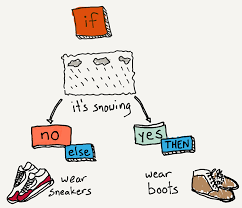
\includegraphics[width=0.3\columnwidth]{Chap04/IfThenElseWearBoots.png}}%
}
\hspace{5pt}%
\subfloat[]{%
    \label{fig:LiDARmap01}%
	\centering
	\setlength{\fboxsep}{0pt}%
\setlength{\fboxrule}{3pt}%
\fbox{
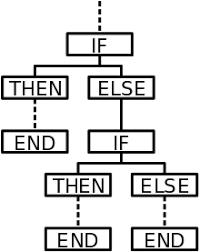
\includegraphics[width=0.3\columnwidth]{Chap04/IfThenEleseWikipedia.png}}%
}
\hspace{5pt}%
\subfloat[]{%
    \label{fig:Regression02}%
	\centering
		\setlength{\fboxsep}{0pt}%
\setlength{\fboxrule}{3pt}%
	\fbox{
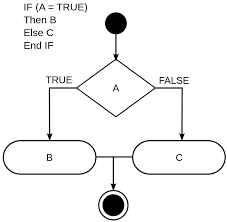
\includegraphics[width=0.32\columnwidth]{Chap04/IfThenEleseWikipedia2.png}}%
}

\caption[]{If statements are also called conditional statements. They allow you to test for a condition before executing a section of code, such as making a recommendation of apparel as a function of the weather. The conditions are always \texttt{\bf T/F} tests. (a) is from \url{https://makecode.microbit.org/courses/csintro/conditionals/overview}, while (b) and (c) are from \url{https://en.wikipedia.org/wiki/Conditional_(computer_programming)}}
    \label{fig:IfThenElse}
\end{figure}


``In computer science, conditionals (that is, conditional statements, conditional expressions and conditional constructs,) are programming language commands for handling decisions;''  see \url{https://en.wikipedia.org/wiki/Conditional_(computer_programming)}. A simple example would be to check for a zero in a denominator before doing a division operation.\\

Julia provides a variety of control flow constructs. Control flow regulates the order of statements to be executed. `if-else` is a common control flow in Julia and other programming languages. The syntax is as follows:
\begin{align*}
if~~ & \textbf{Boolean is \textbf{T}}   \\
& **\texttt{Execute statement block} 1** \\
& **\texttt{Execute statement block} 1** \\
else\\    
& **\texttt{Execute statement block} 2** \\
& **\texttt{Execute statement block} 2** \\
& ** \texttt{Execute statement block} 2** \\
end
\end{align*}

\begin{rem}
Note that in Julia, as in MATLAB, \texttt{\bf then} never appears as a key word! It is implied. 
The first \textbf{true ``if'' or ``elseif''} condition is executed, and then the entire block of \textbf{if statements} is exited. Nothing further is evaluated. If you do not include an \textbf{else} before the end statement, then, if all of the \textbf{if condtions} fail, nothing will be done. This is often very useful, for example, when checking for potential errors in the incoming data to a function. 
\end{rem}

\begin{lstlisting}[language=Julia,style=mystyle]
if (Boolean 1)
    **statement block 1**
elseif (Boolean 2)
    **statement block 2**
elseif (Boolean 3)
    **statement block 3**
...
elseif (Boolean N-1)
    **statement block N-1**
else # nothing goes here
    **statement block N**
end
\end{lstlisting}
% \textbf{Output} 
% \begin{verbatim}

% \end{verbatim}


\begin{lstlisting}[language=Julia,style=mystyle]
# Our first if then else statement
#
# If the condition is evaluated to be true, execute statement1, 
# otherwise, execute statement2
x = sqrt(2)
y = pi/2
if x < y # testing the Boolean (x < y)
    println("x is less than y")
else
    println("x is not less than y")
end
\end{lstlisting}
\textbf{Output} 
\begin{verbatim}
x is less than y
\end{verbatim}

You can string together multiple Boolean conditions, like so. 

\begin{lstlisting}[language=Julia,style=mystyle]
# More conditions can be evaluated using elseif
x = 1
y = 1
if x < y
    println("x is less than y")
elseif x > y
    println("x is greater than y")
else
    println("x is equal to y")
end
\end{lstlisting}
\textbf{Output} 
\begin{verbatim}
x is equal to y
\end{verbatim}

And it is OK to skip the \texttt{else} statement. 


\begin{lstlisting}[language=Julia,style=mystyle]
# It is optional to include the else 
#
x = 1.4142-sqrt(2)
y = NaN
if x < 0
    y = -x
end
[x y]
\end{lstlisting}
\textbf{Output} 
\begin{verbatim}
1×2 Matrix{Float64}:
 -1.35624e-5  1.35624e-5
\end{verbatim}

\begin{example}
Write an ``if statement'' that tests if a variable \texttt{x} is a 1-element vector or not, and when it is a 1-element vector, redefines it as a scalar.
\end{example}

\textbf{Solution}
We first test the \texttt{length} of \texttt{x}. When the length is greater than one, we do nothing. If the length equals one, we then test if \texttt{x} has \texttt{Type} Vector. If it does, we extract its first element to create a scalar.\\


\begin{lstlisting}[language=Julia,style=mystyle]
x=[pi]
# x = pi # uncomment and run, comparing to x = [pi]
@show string(typeof(x))
@show string(typeof(x))[1:6]
if length(x) == 1
    if string(typeof(x))[1:6] == "Vector" # Double equals means EQUIVALENT TO
        @show x=x[1]
        @show typeof(x)
    else
        @show x
    end
end
x
\end{lstlisting}
\textbf{Output} 
\begin{verbatim}
string(typeof(x)) = "Vector\{Irrational\{:\pi\}\}"
(string(typeof(x)))[1:6] = "Vector"
x = x[1] = \pi
typeof(x) = Irrational\{:\pi\}

\pi = 3.1415926535897...
\end{verbatim}

\section{Writing Better Functions}

``A function is a block of organized code that is used to perform a single task. [Functions] provide better modularity for your application and reuse-ability. Depending on the programming language, a function may be called a subroutine, a procedure, a routine, a method, or a subprogram. The generic term, callable unit, is sometimes used. Using functions can allow you to be able to keep your code clean and organized, making it easy to read, and allows the debugging process to be easier;'' from 
\url{https://en.wikiversity.org/wiki/Programming_Fundamentals/Functions}.\\

In Julia, the keywords are \texttt{function}, \texttt{return}, and \texttt{end}. Here we show a very simple function that takes in a variable $x$ and returns $y= x + \pi x^2$.

\begin{lstlisting}[language=Julia,style=mystyle]
# A simple function using the keywords FUNCTION, END, and RETURN
function f(x)
    y = x+pi*x^2
    return y
end
# Call the function
f(2)
\end{lstlisting}
\textbf{Output} 
\begin{verbatim}
14.566370614359172
\end{verbatim}

You can also return more than one value, as in the following example, which also illustrates that any commands that follow the first \texttt{return} statement are ignored.\\

\begin{lstlisting}[language=Julia,style=mystyle]
#
function f(x)
    y = x+pi*x^2
    z = sin(x) + 27*x^3
    return y,z
    w=x+2 # a superfluous line that will be completely ignored 
end
# All operations after the return keyword will be ignored
#
# Call the function
f(3)
\end{lstlisting}
\textbf{Output} 
\begin{verbatim}
(31.274333882308138, 729.1411200080598)
\end{verbatim}

Here is a function that determines the absolute value of a scalar.  \\

\begin{lstlisting}[language=Julia,style=mystyle]
# Build your own absolute value function
function myAbs(a)
    if a >= 0
        return a
    else
        return -a
    end
end
# Call the function
@show myAbs(-2)
@show myAbs(-2.0)
\end{lstlisting}
\textbf{Output} 
\begin{verbatim}
myAbs(-2) = 2
myAbs(-2.0) = 2.0

2.0
\end{verbatim}
Julia has its own built-in \texttt{maximum} function. We'll build our own function just to show how it can be done.

\begin{lstlisting}[language=Julia,style=mystyle]
# Define a more useful function with multiple returns
function myMax(input_vector)
    # initialize the max to the first element 
    # then update when we find a bigger element
    maximum_value = input_vector[1]
    maximum_index = 1
    for i = 1:length(input_vector)
        if input_vector[i] > maximum_value
            maximum_value = input_vector[i]
            maximum_index = i
        end
    end
    return maximum_value, maximum_index
end
\end{lstlisting}
\textbf{Output} 
\begin{verbatim}
myMax (generic function with 1 method)
\end{verbatim}

When we test it, we obtain the maximum value as well as the index of the vector where the maximum value is stored. 
\begin{lstlisting}[language=Julia,style=mystyle]
# Test the function
a = [0, 1, 5, 3.0]
maximum_value, maximum_index = myMax(a)
\end{lstlisting}
\textbf{Output} 
\begin{verbatim}
(5.0, 3)
\end{verbatim}

What if we use a single variable name for the output of the function? 
\begin{lstlisting}[language=Julia,style=mystyle]
# Test the function
a = [0, 1, 5, 3.0]
Answer = myMax(a)
\end{lstlisting}
\textbf{Output} 
\begin{verbatim}
(5.0, 3)
\end{verbatim}

Then \texttt{Answer} is a \texttt{Tuple}. Note that \texttt{Answer[1]} holds the maximum value and \texttt{Answer[2]} holds the index.\\

\begin{lstlisting}[language=Julia,style=mystyle]
@show Answer[1]
Answer[2]
\end{lstlisting}
\textbf{Output} 
\begin{verbatim}
Answer[1] = 5.0

3
\end{verbatim}

\section{A Function for Multiplying Matrices}

Julia has a built-in matrix multiplication function, $A*B$. Just for practice, we'll build a function that uses the method of Chapter 4 in our textbook, where we sum over the product of the columns of $A$ times the rows of $B$.  We will then verify that our function gives the same answer as the usual method of doing matrix multiplication. 

\begin{lstlisting}[language=Julia,style=mystyle]
function myMatrixMultiply(A,B)
    nRowsA, nColsA = size(A)
    nRowsB, nColsB = size(B)
    if nColsA != nRowsB
        println("Error: Matrix sizes are not compatible for multiplication")
        C=NaN
        return C
    end
    C=zeros(nRowsA,nColsB)
    for i = 1:nColsA
        C = C + A[:,i]*B[i:i,:]
    end
    return C
end
\end{lstlisting}
\textbf{Output} 
\begin{verbatim}
myMatrixMultiply (generic function with 1 method)
\end{verbatim}


\begin{lstlisting}[language=Julia,style=mystyle]
# test of myMatrixMultiply(A,B)
using Random
Random.seed!(4321)
A=randn(3,4)
B=randn(4,5)

C=myMatrixMultiply(A,B)
# Matrix of zeros means we got it right!
C-A*B  
\end{lstlisting}
\textbf{Output} 
\begin{verbatim}
3×5 Matrix{Float64}:
  0.0          2.22045e-16  0.0   0.0           0.0
 -1.11022e-16  0.0          0.0   0.0           1.11022e-16
  0.0          0.0          0.0  -2.22045e-16  -5.55112e-17
\end{verbatim}

The next function implements matrix multiplication the way it is done in Julia.\\


\begin{lstlisting}[language=Julia,style=mystyle]
function myMatrixMultiplyOrdinary(A,B)
    nRowsA, nColsA = size(A)
    nRowsB, nColsB = size(B)
    if nColsA != nRowsB
        println("Error: Matrix sizes are not compatible for multiplication")
        C=NaN
        return C
    end
    C=zeros(nRowsA,nColsB)
    for i = 1:nRowsA
        for j = 1:nColsB
            C[i,j] = (A[i:i,:]*B[:,j])[1]
        end
    end
    return C
end
\end{lstlisting}
\textbf{Output} 
\begin{verbatim}
myMatrixMultiplyOrdinary (generic function with 1 method)
\end{verbatim}


\begin{lstlisting}[language=Julia,style=mystyle]
# test of myMatrixMultiplyOrdinary(A,B)
using Random
Random.seed!(4321)
A=randn(3,4)
B=randn(4,5)

C=myMatrixMultiplyOrdinary(A,B)
# Matrix of zeros means we got it right!
C-A*B
\end{lstlisting}
\textbf{Output} 
\begin{verbatim}
3×5 Matrix{Float64}:
  0.0          0.0  0.0  0.0  0.0
 -1.11022e-16  0.0  0.0  0.0  0.0
  0.0          0.0  0.0  0.0  0.0
\end{verbatim}




\section{Forward Substitution}

This is how to solve $Ax = b$ when $A$ is a square lower triangular matrix, with no zeros on the diagonal. See Chapter 3 of the ROB 101 Textbook.

\begin{lstlisting}[language=Julia,style=mystyle]
using LinearAlgebra
function forwardsub(L, b)
    # Assert no entries on the diagonal of U
    # are 0 (or very close to 0)
    @assert minimum(abs.(diag(L))) > 1e-4
    # START of our computations
    n = length(b)
    x = Vector{Float64}(undef, n); #initialize vector x to the correct size
    x[1] = b[1]/L[1,1] #find the first entry of x
    for i = 2:n #find every entry from the 2nd to the end
        x[i]=( b[i] - (L[i,1:i-1])'*x[1:i-1] )/L[i,i] 
        #notice that we used a transpose operator to get the row of L
    end
    # END of our computations.
    return x
end
\end{lstlisting}
\textbf{Output} 
\begin{verbatim}
forwardsub (generic function with 1 method)
\end{verbatim}

Here we work an example with 300 variables. \\


\begin{lstlisting}[language=Julia,style=mystyle]
using Random
Random.seed!(4321)
N=300
L=rand(N,N)
for i = 1:N
    L[i,(i+1):N] = 0.0 * L[i,(i+1):N]
    L[i,i]=1.0
end
b=randn(N,1)
x=forwardsub(L, b)
#x = inv(L)*b
norm(L*x-b)
\end{lstlisting}
\textbf{Output} 
\begin{verbatim}
1.303218919812078e-9
\end{verbatim}


\begin{figure}[htb!]%
\centering
\subfloat[]{%
    \label{fig:Regression03}%
	\centering
		\setlength{\fboxsep}{0pt}%
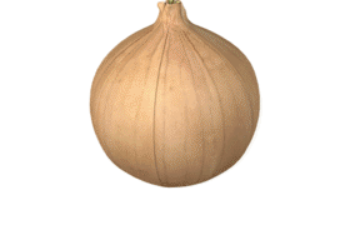
\includegraphics[width=0.31\columnwidth]{graphics/Chap04/PeelOnion1.png}}%
\hspace{5pt}%
\subfloat[]{%
    \label{fig:LiDARmap03}%
	\centering
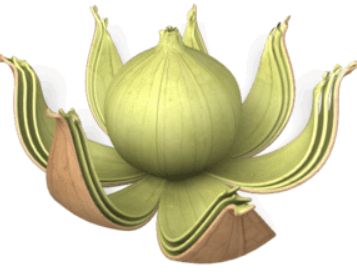
\includegraphics[width=0.30\columnwidth]{Chap04/PeelOnion2.png}}%
\hspace{5pt}%
\subfloat[]{%
    \label{fig:Regression04}%
	\centering
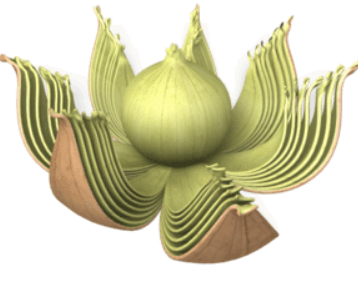
\includegraphics[width=0.31\columnwidth]{Chap04/PeelOnion3.png}}%


\caption[]{We will take a matrix apart, row by row, column by column, until there is nothbing left but zeros. Images are snapshots from \url{https://content.presentermedia.com/content/animsp/00021000/21530/onion_layers_300_wht.gif}.}
    \label{fig:Onion}
\end{figure}

\section{Peeling the Onion: the Base Step for LU Factorization}
\label{sec:PeelingOnions}

This material is tied to Chapter 5 of the ROB 101 Textbook. ``Peeling the Onion'' is an elementary step in factoring a matrix into the product of a lower triangular matrix $L$ and an upper triangular matrix $U$. We will build a function that peels one layer of a matrix at a time. It will work for the special case that the ``pivot'' element is non-zero. Chapter 5 explains how to modify the process when the ``pivot'' is zero, in case you are curious!\\

Consider the square matrix 
$$M_0=\left[\begin{array}{rrr} 
    1   &  4   &  5 \\
     2  &   9  &  17 \\
     3  &  18  &  58 \end{array}  \right]. $$
Our goal is to find a column vector $C_1$ and a row vector $R_1$ such that  
$$M-C_1 \cdot R_1 = \left[\begin{array}{rrr} 
    0  &  0   &  0 \\
     0  &   \ast &  \ast \\
    0  &  \ast  &  \ast \end{array}  \right], $$   
where $\ast$ denotes ``don't care'' in the sense that we do not care about their particular values. Another way to say this is, we want to zero out the first column and the first row of $M$. That means, $C_1$ and $R_1$ are chosen so that the first column and first row of their matrix product $C_1 \cdot R_1$ match the first column and first row of $M$.\\

To see that this is possible, observe that
\begin{align*}
M_0  =\left[\begin{array}{rrr} 
\RED     1   & \RED   4   & \RED  5 \\
 \RED     2  &   9  &  17 \\
 \RED     3  &  18  &  58 \end{array}  \right] &= \underbrace{\left[
\begin{array}{ccc}
\RED 0.0 & \RED 0.0 & \RED 0.0 \\
\RED 0.0 & 1.0 & 7.0 \\
\RED 0.0 & 6.0 & 43.0 \\
\end{array}
\right]}_{M_1} + \underbrace{\left[
\begin{array}{c}
1.0 \\
2.0 \\
3.0 \\
\end{array}
\right]}_{C_1} \cdot \underbrace{\left[
\begin{array}{ccc}
1.0 & 4.0 & 5.0 \\
\end{array}
\right]}_{R_1} \\
& = \underbrace{\left[
\begin{array}{ccc}
\RED 0.0 & \RED 0.0 & \RED 0.0 \\
\RED 0.0 & 1.0 & 7.0 \\
\RED 0.0 & 6.0 & 43.0 \\
\end{array}
\right]}_{M_1}  + \underbrace{\left[
\begin{array}{ccc}
\RED  1.0 &\RED  4.0 &\RED  5.0 \\
\RED 2.0 & 8.0 & 10.0 \\
\RED 3.0 & 12.0 & 15.0 \\
\end{array}
\right]}_{C_1 \cdot R_1}
\end{align*} 
where we arrive at $M_1$ after \textcolor{red}{\bf  ``Peeling off the First Row and First Column''} of $M_0$.\\

Furthermore, we can write 
\begin{align*}
M_1=\left[
\begin{array}{ccc}
 0.0 &  0.0 &  0.0 \\
 0.0 & \RED 1.0 & \RED 7.0 \\
 0.0 & \RED 6.0 & 43.0 \\
\end{array}
\right] & = \underbrace{\left[
\begin{array}{ccc}
0.0 & 0.0 & 0.0 \\
0.0 & \RED 0.0 & \RED 0.0 \\
0.0 & \RED 0.0 & 1.0 \\
\end{array}
\right]}_{M_2} + \underbrace{\left[
\begin{array}{c}
0.0 \\
1.0 \\
6.0 \\
\end{array}
\right]}_{C_2} \cdot \underbrace{\left[
\begin{array}{ccc}
0.0 & 1.0 & 7.0 \\
\end{array}
\right]}_{R_2} \\
& = \underbrace{
\left[
\begin{array}{ccc}
0.0 & 0.0 & 0.0 \\
0.0 & \RED 0.0 & \RED 0.0 \\
0.0 & \RED 0.0 & 1.0 \\
\end{array}
\right]
}_{M_2}  + \underbrace{
\left[
\begin{array}{ccc}
0.0 & 0.0 & 0.0 \\
0.0 & \RED 1.0 & \RED 7.0 \\
0.0 & \RED 6.0 & 42.0 \\
\end{array}
\right]
}_{C_2 \cdot R_2}
\end{align*}
where we arrive at $M_2$ after \textcolor{red}{\bf ``Peeling off the Second Row and Second Column''} of $M_1$. \\


Finally, we can write 
\begin{align*}
M_2=\left[
\begin{array}{ccc}
0.0 & 0.0 & 0.0 \\
0.0 &  0.0 &  0.0 \\
0.0 &  0.0 & \RED 1.0 \\
\end{array}
\right] & = \underbrace{
\left[
\begin{array}{ccc}
0.0 & 0.0 & 0.0 \\
0.0 & 0.0 & 0.0 \\
0.0 & 0.0 & \RED 0.0 \\
\end{array}
\right]
}_{M_3} + \underbrace{\left[
\begin{array}{c}
0.0 \\
0.0 \\
1.0 \\
\end{array}
\right]}_{C_3} \cdot \underbrace{\left[
\begin{array}{ccc}
0.0 & 0.0 & 1.0 \\
\end{array}
\right]}_{R_3} \\
& = \underbrace{
\left[
\begin{array}{ccc}
0.0 & 0.0 & 0.0 \\
0.0 &  0.0 &  0.0 \\
0.0 &  0.0 & \RED 0.0 \\
\end{array}
\right]
}_{M_3}  + \underbrace{
\left[
\begin{array}{ccc}
0.0 & 0.0 & 0.0 \\
0.0 & 0.0 & 0.0 \\
0.0 & 0.0 & \RED 1.0 \\
\end{array}
\right]
}_{C_3 \cdot R_3}
\end{align*}
where we arrive at $M_3$ after \textcolor{red}{\bf ``Peeling off the Third Row and Third Column''} of $M_2$. Because $M_3$ is the zero matrix, the process stops.\\

We have arrived at 
\begin{align*}
M_0  =\left[\begin{array}{rrr} 
    1   &  4   &  5 \\
    2  &   9  &  17 \\
    3  &  18  &  58 \end{array}  \right] &=\underbrace{\left[
\begin{array}{c}
1.0 \\
2.0 \\
3.0 \\
\end{array}
\right]}_{C_1} \cdot \underbrace{\left[
\begin{array}{ccc}
1.0 & 4.0 & 5.0 \\
\end{array}
\right]}_{R_1} +  \underbrace{\left[
\begin{array}{c}
0.0 \\
1.0 \\
6.0 \\
\end{array}
\right]}_{C_2} \cdot \underbrace{\left[
\begin{array}{ccc}
0.0 & 1.0 & 7.0 \\
\end{array}
\right]}_{R_2}  + \underbrace{\left[
\begin{array}{c}
0.0 \\
0.0 \\
1.0 \\
\end{array}
\right]}_{C_3} \cdot \underbrace{\left[
\begin{array}{ccc}
0.0 & 0.0 & 1.0 \\
\end{array}
\right]}_{R_3} \\
& = \underbrace{\left[
\begin{array}{ccc}
1.0 & 0.0 & 0.0 \\
2.0 & 1.0 & 0.0 \\
3.0 & 6.0 & 1.0 
\end{array}
\right]}_{\begin{array}{ccc}
C_1 & C_2 & C_3 \\
\end{array}} \cdot \left. \left[
\begin{array}{ccc}
1.0 & 4.0 & 5.0 \\
0.0 & 1.0 & 7.0 \\
0.0 & 0.0 & 1.0 \\
\end{array}
\right]\right\} \begin{array}{c}
R_1 \\
R_2 \\
R_3 \\
\end{array} \\
& = L \cdot U
\end{align*} 

\textbf{How do we find the column vectors $C_i$ and the row vectors $R_i$, for $1 \le i \le 3$? We have an algorithm for that.}\\

\begin{lstlisting}[language=Julia,style=mystyle]
function peel_one_layer(Temp, k)
    # k is the layer we are peeling (row and column)
    # Temp is the matrix from which we are
    # peeling the k-th row and k-th column
    # We assume layers 1:k-1 are already zeroed
    pivot = Temp[k, k] # We assume pivot != 0
    C = Temp[:, k] / pivot  # Normalized k-th column
    R = Temp[k:k, :]        # k-th row, no normalization
    Temp = Temp - C*R
    return C, R, Temp
end
\end{lstlisting}
\textbf{Output} 
\begin{verbatim}
peel_one_layer (generic function with 1 method)
\end{verbatim}

Now, let's apply our function.

\begin{lstlisting}[language=Julia,style=mystyle]
M0=[1.0 4 5; 2 9 17; 3 18 58]
C1,R1,M1=peel_one_layer(M0, 1) # layer 1
@show C1
@show R1
M1
\end{lstlisting}
\textbf{Output} 
\begin{verbatim}
C1 = [1.0, 2.0, 3.0]
R1 = [1.0 4.0 5.0]

3×3 Matrix{Float64}:
 0.0  0.0   0.0
 0.0  1.0   7.0
 0.0  6.0  43.0
\end{verbatim}

Note that we ``peeled off'' the first column and row.

\begin{lstlisting}[language=Julia,style=mystyle]
C2,R2,M2=peel_one_layer(M1, 2) # layer 2
@show C2
@show R2
M2
\end{lstlisting}
\textbf{Output} 
\begin{verbatim}
C2 = [0.0, 1.0, 6.0]
R2 = [0.0 1.0 7.0]

3×3 Matrix{Float64}:
 0.0  0.0  0.0
 0.0  0.0  0.0
 0.0  0.0  1.0
\end{verbatim}

Note that we ``peeled off'' the second column and row.

\begin{lstlisting}[language=Julia,style=mystyle]
C3,R3,M3=peel_one_layer(M2, 3) # layer 3
@show C3
@show R3
M3
\end{lstlisting}
\textbf{Output} 
\begin{verbatim}
C3 = [0.0, 0.0, 1.0]
R3 = [0.0 0.0 1.0]

3×3 Matrix{Float64}:
 0.0  0.0  0.0
 0.0  0.0  0.0
 0.0  0.0  0.0
\end{verbatim}

We arrived at a matrix of zeros. Next, we form a lower triangular matrix, $L$\\

\begin{lstlisting}[language=Julia,style=mystyle]
L=[C1 C2 C3]
\end{lstlisting}
\textbf{Output} 
\begin{verbatim}
3×3 Matrix{Float64}:
 1.0  0.0  0.0
 2.0  1.0  0.0
 3.0  6.0  1.0
\end{verbatim}

and an upper triangular matrix, $U$\\
\begin{lstlisting}[language=Julia,style=mystyle]
U = [R1;R2;R3]
\end{lstlisting}
\textbf{Output} 
\begin{verbatim}
3×3 Matrix{Float64}:
 1.0  4.0  5.0
 0.0  1.0  7.0
 0.0  0.0  1.0
\end{verbatim}

We now show that $M_0 = L \cdot U$,\\

\begin{lstlisting}[language=Julia,style=mystyle]
M0-L*U
\end{lstlisting}
\textbf{Output} 
\begin{verbatim}
3×3 Matrix{Float64}:
 0.0  0.0  0.0
 0.0  0.0  0.0
 0.0  0.0  0.0
\end{verbatim}

We can place our function \texttt{peel\_one\_layer(Temp, k)} in a \texttt{for\,loop} to compute an LU Factorization when row permutation is not required.

\begin{lstlisting}[language=Julia,style=mystyle]
function myLU(A)
    Temp = copy(A) # Initialize Temp matrix by 
                #copying the original matrix A
    nRows, nCols = size(Temp) # Get the size of the input matrix
    K = minimum([nRows, nCols])
    # Initialize the lower and upper triangular matrix
    L = zeros(Float64, (nRows, K)) # Using zeros function by
                                # specifying both type and size
    U = zeros(Float64, (K, nCols)) 
    # Here we do the actual factorization
    for k = 1:K
        C, R, Temp = peel_one_layer(Temp, k)
        L[:, k] = C
        U[k:k, :] = R
    end
    return L, U
end
\end{lstlisting}
\textbf{Output} 
\begin{verbatim}
myLU (generic function with 1 method)
\end{verbatim}


\begin{lstlisting}[language=Julia,style=mystyle]
using Random
using LinearAlgebra
Random.seed!(09182022)
A = randn(5, 7)
#
L, U = myLU(A)
\end{lstlisting}
\textbf{Output} 
\begin{verbatim}
([1.0 -0.0 … 0.0 -0.0; 1.3841751352784288 1.0 … 0.0 -0.0; … ; 
1.8240441684383097 1.7669720431792901 … 1.0 -0.0; 
1.1660675070497575 0.4629237529415664 … -0.8475551711339656 1.0], 
[-0.3236905701556438 0.9372755784538437 … -0.009357226530146447 -0.0076384514441543774;
0.0 -2.1005108102249452 … 1.4460922800584077 0.41893233388727713;
… ; 0.0 0.0 … 0.19792290864355966 -0.6285612979102336;
-5.551115123125783e-17 0.0 … -1.3304631421106152 1.0052145594104471])
\end{verbatim}

The above output is hard to read. It is better if you look at \texttt{L} and \texttt{U} in separate cells.

\begin{lstlisting}[language=Julia,style=mystyle]
L
\end{lstlisting}
\textbf{Output} 
\begin{verbatim}
5×5 Matrix{Float64}:
 1.0      -0.0        0.0        0.0       -0.0
 1.38418   1.0        0.0        0.0       -0.0
 8.38948   4.18061    1.0        0.0       -0.0
 1.82404   1.76697    0.271808   1.0       -0.0
 1.16607   0.462924  -0.135905  -0.847555   1.0
\end{verbatim}


\begin{lstlisting}[language=Julia,style=mystyle]
U
\end{lstlisting}
\textbf{Output} 
\begin{verbatim}
5×7 Matrix{Float64}:
 -0.323691      0.937276   0.578516  … 0.487937  -0.00935723  -0.00763845
  0.0          -2.10051   -1.18148      -0.516585   1.44609      0.418932
  0.0           0.0        2.42504      -1.45327   -6.78688     -1.58847
  0.0           0.0        0.0           0.717684   0.197923    -0.628561
 -5.55112e-17   0.0        0.0          -2.41577   -1.33046      1.00521
\end{verbatim}

\begin{lstlisting}[language=Julia,style=mystyle]
A-L*U
\end{lstlisting}
\textbf{Output} 
\begin{verbatim}
5×7 Matrix{Float64}:
 0.0   0.0           0.0          0.0          … 0.0           0.0
 0.0   0.0           0.0          6.93889e-17      0.0           0.0
 0.0  -4.44089e-16  -4.44089e-16  6.66134e-16     -4.44089e-16  -5.55112e-17
 0.0  -4.44089e-16  -1.11022e-16  5.55112e-17      3.33067e-16   0.0
 0.0   1.38778e-17   8.32667e-17  0.0              1.38778e-16   0.0
\end{verbatim}

\section{Debugging}

We'll introduce errors into a few of the functions and if-then-else statements we have used in the Chapter and see how the ``bugs''  manifest themselves. \\

\subsection{Misusing operations designed for scalar variables}
Here is a function designed for $x$ a real number.

\begin{lstlisting}[language=Julia,style=mystyle]
function f(x)
    y = x+pi*x^2
    return y
end
\end{lstlisting}
\textbf{Output} 
\begin{verbatim}
f (generic function with 1 method)
\end{verbatim}

We forget that we designed it for a real number and try to apply it to a vector.

\begin{lstlisting}[language=Julia,style=mystyle]
f([1;2])
\end{lstlisting}
\textbf{Output} 
\begin{verbatim}
MethodError: no method matching ^(::Vector{Int64}, ::Int64)
Closest candidates are:
  ^(::Union{AbstractChar, AbstractString}, ::Integer) at strings/basic.jl:718
  ^(::Complex{var"#s79"} where var"#s79"<:AbstractFloat, ::Integer) at complex.jl:818
  ^(::Complex{var"#s79"} where var"#s79"<:Integer, ::Integer) at complex.jl:820
  ...

Stacktrace:
 [1] macro expansion
   @ ./none:0 [inlined]
 [2] literal_pow
   @ ./none:0 [inlined]
 [3] f(x::Vector{Int64})
   @ Main ./In[1]:2
 [4] top-level scope
   @ In[2]:1
 [5] eval
   @ ./boot.jl:360 [inlined]
 [6] include_string(mapexpr::typeof(REPL.softscope), mod::Module, 
 code::String, filename::String)
   @ Base ./loading.jl:1094

\end{verbatim}

In the above error message, \texttt{top-level scope, ~@ In[1]:2 } is referring to the Cell where we defined the function. The message ``\textcolor{red}{\bf MethodError: no method matching $ \wedge $(::Vector{Int64}, ::Int64)}'' is telling us that Julia does not know how to compute the square of a vector. There are two solutions to this. 


\begin{lstlisting}[language=Julia,style=mystyle]
f.([1;2]) # Solution 1 is to apply broadcasting
\end{lstlisting}
\textbf{Output} 
\begin{verbatim}
2-element Vector{Float64}:
  4.141592653589793
 14.566370614359172
\end{verbatim}

\begin{lstlisting}[language=Julia,style=mystyle]
function f(x)
    y = x .+ pi * x.^2 # Solution 2 is make the function work for vectors or scalars
    return y
end

f([1;2])
\end{lstlisting}
\textbf{Output} 
\begin{verbatim}
2-element Vector{Float64}:
  4.141592653589793
 14.566370614359172
\end{verbatim}

\subsection{Bounds Error}

We recall our function for multiplying matrices.

\begin{lstlisting}[language=Julia,style=mystyle]
function myMatrixMultiply(A,B)
    nRowsA, nColsA = size(A)
    nRowsB, nColsB = size(B)
    if nColsA != nRowsB
        println("Error: Matrix sizes are not compatible for multiplication")
        C=NaN
        return C
    end
    C=zeros(nRowsA,nColsB)
    for i = 1:nColsA
        C = C + A[:,i]*B[i:i,:]
    end
    return C
end

\end{lstlisting}
\textbf{Output} 
\begin{verbatim}
myMatrixMultiply (generic function with 1 method)
\end{verbatim}

We give the function what looks like perfectly good data.

\begin{lstlisting}[language=Julia,style=mystyle]
A=[1 2 3 4]
B=[2;3;4;5.0]
myMatrixMultiply(A,B)
\end{lstlisting}
\textbf{Output} 
\begin{verbatim}
BoundsError: attempt to access Tuple{Int64} at index [2]

Stacktrace:
 [1] indexed_iterate
   @ ./tuple.jl:86 [inlined]
 [2] myMatrixMultiply(A::Matrix{Int64}, B::Vector{Float64})
   @ Main ./In[6]:3
 [3] top-level scope
   @ In[7]:3
 [4] eval
   @ ./boot.jl:360 [inlined]
 [5] include_string(mapexpr::typeof(REPL.softscope), mod::Module, 
 code::String,  filename::String)
   @ Base ./loading.jl:1094
\end{verbatim}

Cell [6] is where we defined the function \texttt{myMatrixMultiply} and line 3 is the command \texttt{nRowsB, nColsB = size(B)}. The problem is that $B$ is a vector and the \texttt{size} command does not return a value for $\rm nColsB$, even though we ``know'' it should be one. \\

In the following, we show two ways to fix this issue. In the first \texttt{if-then-else} statement, we make use of Types in Julia. In the second \texttt{if-then-else} statement, we exploit the fact that if $B$ is a matrix, then \texttt{size(B)} has two components, and hence its length is two, and when $B$ is a vector or scalar, \texttt{size(B)} will have length one. This is certainly the simpler solution of the two. \textcolor{blue}{\bf An even simpler solution is only to call the function with matrix arguments!}  

\begin{lstlisting}[language=Julia,style=mystyle]
function myMatrixMultiply(A,B)
    if (typeof(A) == Matrix{Int64})||(typeof(A) == Matrix{Float64})
        nRowsA, nColsA = size(A)
    else
        nRowsA = length(A)
        nColsA = 1
    end

    if length(size(B)) == 2
        nRowsB, nColsB = size(B)
    else
        nRowsB = length(B)
        nColsB = 1
    end
    if nColsA != nRowsB
        @show nColsA
        @show nRowsB
        println("Error: Matrix sizes are not compatible for multiplication")
        C=NaN
        return C
    end
    C=zeros(nRowsA,nColsB)
    for i = 1:nColsA
        C = C + A[:,i]*B[i:i,:]
    end
    return C
end
\end{lstlisting}
\textbf{Output} 
\begin{verbatim}
myMatrixMultiply (generic function with 1 method)
\end{verbatim}


\begin{lstlisting}[language=Julia,style=mystyle]
myMatrixMultiply(A,B)
\end{lstlisting}
\textbf{Output} 
\begin{verbatim}
1×1 Matrix{Float64}:
 40.0
\end{verbatim}

\subsection{Using the display( ) command to find an error buried in a function}

We insert an error in a function that worked just fine for us in Chapter~\ref{sec:PeelingOnions}. Can you spot the error before we run the function? 

\begin{lstlisting}[language=Julia,style=mystyle]
function peel_one_layer(Temp, k)
# k is the layer we are peeling (row and column)
# Temp is the matrix from which we are
# peeling the k-th row and k-th column
    pivot = Temp[k, k]
    C = Temp[:, k] # kth column
    # next we normalize
    C = C / pivot # We assume pivot != 0
    R = Temp[k, :]  # kth row
    Temp = Temp - C*R
    return C, R, Temp
end
\end{lstlisting}
\textbf{Output} 
\begin{verbatim}
peel_one_layer (generic function with 1 method)
\end{verbatim}

\begin{lstlisting}[language=Julia,style=mystyle]
Temp=[1.0 2; 3 4]
display(Temp)
C, R, Temp = peel_one_layer(Temp, 1)
\end{lstlisting}
\textbf{Output} 
\begin{verbatim}
2×2 Matrix{Float64}:
 1.0  2.0
 3.0  4.0
 
MethodError: no method matching *(::Vector{Float64}, ::Vector{Float64})
Closest candidates are:
  *(::Any, ::Any, ::Any, ::Any...) at operators.jl:560
  *(::StridedMatrix{T}, ::StridedVector{S}) where 
  {T<:Union{Float32, Float64, ComplexF32, ComplexF64}, S<:Real} at
  /buildworker/worker/package_linux64/build/usr/share/julia/stdlib/v1.6/
LinearAlgebra/src/matmul.jl:44
  *(::StridedVecOrMat{T} where T, ::LinearAlgebra.Adjoint{var"#s832", var"#s831"} 
  where {var"#s832", var"#s831"<:LinearAlgebra.LQPackedQ}) at 
  /buildworker/worker/package_linux64/build/usr/share/julia/stdlib
  /v1.6/LinearAlgebra/src/lq.jl:254
  ...

Stacktrace:
 [1] peel_one_layer(Temp::Matrix{Float64}, k::Int64)
   @ Main ./In[49]:10
 [2] top-level scope
   @ In[52]:3
 [3] eval
   @ ./boot.jl:360 [inlined]
 [4] include_string(mapexpr::typeof(REPL.softscope), mod::Module, code::String, 
 filename::String)
   @ Base ./loading.jl:1094
\end{verbatim}

The message \texttt{no method matching *(::Vector{Float64}, ::Vector{Float64})} is telling us that Julia does not know how to multiply two vectors. We are surprised by this message because we think, in line 10 of our function (from the message \texttt{In[49]:10}) that we are multiplying a column vector $C$ times a row vector $R$, which is a legitimate operation. \textcolor{red}{\bf To find the error, we use the \texttt{display} command} (you could also have used the \texttt{@show} command).


\begin{lstlisting}[language=Julia,style=mystyle]
function peel_one_layer(Temp, k)
# k is the layer we are peeling (row and column)
# Temp is the matrix from which we are
# peeling the k-th row and k-th column
    pivot = Temp[k, k]
    C = Temp[:, k] # kth column
    # next we normalize
    C = C / pivot # We assume pivot != 0
    R = Temp[k, :]  # kth row
    display(C)
    display(R)
    Temp = Temp - C*R
    return C, R, Temp
end

C, R, Temp = peel_one_layer(Temp, 1)
\end{lstlisting}
\textbf{Output} 
\begin{verbatim}
2-element Vector{Float64}:
 1.0
 3.0
2-element Vector{Float64}:
 1.0
 2.0
MethodError: no method matching *(::Vector{Float64}, ::Vector{Float64})
\end{verbatim}

Sure enough, $R$ is a column vector. And we note that we should have used \texttt{    R = Temp[k:k, :]} to extract a row and keep it a row.\\

If we use the \texttt{@show} command, we get the same information but it's less direct in that we have to recognize that \texttt{R = [1.0, 2.0]} is a column vector due to the comma separating the two entries.

\begin{lstlisting}[language=Julia,style=mystyle]
function peel_one_layer(Temp, k)
# k is the layer we are peeling (row and column)
# Temp is the matrix from which we are
# peeling the k-th row and k-th column
    pivot = Temp[k, k]
    C = Temp[:, k] # kth column
    # next we normalize
    C = C / pivot # We assume pivot != 0
    R = Temp[k, :]  # kth row
    @show C
    @show R
    Temp = Temp - C*R
    return C, R, Temp
end

C, R, Temp = peel_one_layer(Temp, 1)
\end{lstlisting}
\textbf{Output} 
\begin{verbatim}
C = [1.0, 3.0]
R = [1.0, 2.0]

MethodError: no method matching *(::Vector{Float64}, ::Vector{Float64})
\end{verbatim}


% \begin{lstlisting}[language=Julia,style=mystyle]

% \end{lstlisting}
% \textbf{Output} 
% \begin{verbatim}

% \end{verbatim}

% \begin{lstlisting}[language=Julia,style=mystyle]

% \end{lstlisting}
% \textbf{Output} 
% \begin{verbatim}

% \end{verbatim}

\section{(Optional Read) ``Hero 60 AD'' or Heron's Formula for the Area of a Triangle}


While everyone knows the formula ${\rm Area} = \frac{1}{2} {\rm base} \times {\rm height}$ for the area of a triangle, very few of us were taught Heron's formula, which avoids the use of trigonometry or geometry to compute the height of the triangle (of course, when it is not a right triangle). We create a function using this formula and then illustrate the programming adage, \textbf{``garbage in, garbage out''}. \\

A derivation of Heron's formula can be found here on YouTube \url{https://www.youtube.com/watch?v=9qbpmYqr4so} or in Wikipedia \url{https://en.wikipedia.org/wiki/Heron\%27s_formula}, where it is pointed out that ``The formula is credited to Heron (or Hero) of Alexandria, and a proof can be found in his book Metrica, written around AD 60. It has been suggested that Archimedes knew the formula over two centuries earlier, and since Metrica is a collection of the mathematical knowledge available in the ancient world, it is possible that the formula predates the reference given in that work.'' Moreover, the Chinese had discovered a similar formula, documented in 1247 \url{https://en.wikipedia.org/wiki/Mathematical_Treatise_in_Nine_Sections}, though it may have been known much earlier.


\begin{figure}[htb!]%
\centering
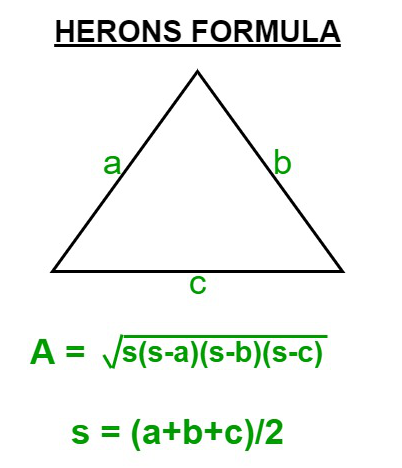
\includegraphics[width=0.31\columnwidth]{graphics/Chap04/heron.jpg}%
\caption[]{Heron's formula for the area of a triangle. Source  \url{https://www.geeksforgeeks.org/herons-formula/}.}
    \label{columneron}
\end{figure}

\begin{lstlisting}[language=Julia,style=mystyle]
function heron(a, b, c)
    s = (a + b + c)/2
    Area = sqrt( s*(s-a)*(s-b)*(s-c) )
    return Area
end
\end{lstlisting}
\textbf{Output} 
\begin{verbatim}
heron (generic function with 1 method)
\end{verbatim}

We now insert the canonical right triangle, (3, 4, 5), where we can take the base as 3 and the height as 2 or the base as 4 and the height as 1.5. In either case, the area is 6.0, and voil\`a, Heron agrees with us! 
\begin{lstlisting}[language=Julia,style=mystyle]
area = heron(3,4,5)
\end{lstlisting}
\textbf{Output} 
\begin{verbatim}
6.0
\end{verbatim}

What about a triangle with side lengths (3, 4, 4.5)? \\

\begin{lstlisting}[language=Julia,style=mystyle]
area = heron(3,4,4.5)
\end{lstlisting}
\textbf{Output} 
\begin{verbatim}
5.881313097429858
\end{verbatim}

Can you correctly compute the area using trigonometry? Go for it! \\

\textcolor{red}{\bf \large Garbage in, garbage out}. What if we insert data into our function where the lengths of the sides are not compatible with forming a triangle, such as (3, 4, 8)?\\

\begin{lstlisting}[language=Julia,style=mystyle]
area = heron(3,4,8)
\end{lstlisting}
\textbf{Output} 
\begin{verbatim}
DomainError with -59.0625:
sqrt will only return a complex result if called with a complex argument. 
Try sqrt(Complex(x)).

Stacktrace:
 [1] throw_complex_domainerror(f::Symbol, x::Float64)
   @ Base.Math ./math.jl:33
 [2] sqrt
   @ ./math.jl:582 [inlined]
 [3] heron(a::Int64, b::Int64, c::Int64)
   @ Main ./In[50]:3
 [4] top-level scope
   @ In[51]:1
 [5] eval
   @ ./boot.jl:360 [inlined]
 [6] include_string(mapexpr::typeof(REPL.softscope), mod::Module, code::String, 
 filename::String)
   @ Base ./loading.jl:1094
\end{verbatim}

The error is on line 3; we tried to take the square root of a negative number. We know if the sum of the two shortest sides exceeds the largest side, then we cannot form a triangle. Let's add this as a check on our function, and while we are at it, also check for negative lengths!\\ 

\begin{lstlisting}[language=Julia,style=mystyle]
function heron(a, b, c)
    # Let's include tests on the inputs to make
    # sure they correspond to a feasible triangle
    #
    data=sort([a; b; c])
    a=data[1]; b=data[2]; c=data[3]
    if a <= 0
        println("Cannot have sides with non-positive length")
        return im # return an imaginary number, just for fun
    elseif c > a + b
        println("Provided data does not form a triangle")
        return im # return an imaginary number, just for fun
    end
    s = (a + b + c)/2 # semi-perimeter
    Area = sqrt( s*(s-a)*(s-b)*(s-c) )
    return Area
end
\end{lstlisting}
\textbf{Output} 
\begin{verbatim}
heron (generic function with 1 method)
\end{verbatim}

The above is a more professional version of our function. \\

\begin{lstlisting}[language=Julia,style=mystyle]
area = heron(3,4,8)
\end{lstlisting}
\textbf{Output} 
\begin{verbatim}
Provided data does not form a triangle

im
\end{verbatim}

The sky is the limit! Here is a version of the function where we can specify the input data in two forms:
\begin{itemize}
    \item as three points in $\real^n$ and then compute the area of the triangle formed by the points, or
    \item as the lengths of the sides, as we did before.
\end{itemize}


\begin{lstlisting}[language=Julia,style=mystyle]
using LinearAlgebra
function heron(A, B, C)
    dim = maximum([length(A), length(B), length(C)])
    if dim > 1
        # Input consists of points in Rn for n >= 2
        if ( length(A) == length(B) )&( length(B) == length(C))
            a=norm(A-B); b = norm(B-C); c = norm(C-A)
            # Lengths will automatically form a triangle
            s = (a + b + c)/2 # semi-perimeter
            Area = sqrt( s*(s-a)*(s-b)*(s-c) )
            return Area
        else
            println("Data is not consistent as points in Rn")
            return im # return an imaginary number, just for fun
        end
    else
        # Input consists of lengths of the sides
        # Check the lengths to make sure
        # they correspond to a feasible triangle
        #
        data=sort([A; B; C])
        a=data[1]; b=data[2]; c=data[3]
        if a <= 0
            println("Cannot have sides with non-positive length")
            return im # return an imaginary number, just for fun
        elseif c > a + b
            println("Provided data does not form a triangle")
            return im # return an imaginary number, just for fun
        end
        s = (a + b + c)/2 # semi-perimeter
        Area = sqrt( s*(s-a)*(s-b)*(s-c) )
        return Area
    end    
end
\end{lstlisting}
\textbf{Output} 
\begin{verbatim}
heron (generic function with 1 method)
\end{verbatim}


\begin{lstlisting}[language=Julia,style=mystyle]
heron([1 2 0], [2 3 5], [4 0 6])
\end{lstlisting}
\textbf{Output} 
\begin{verbatim}
9.513148795220223
\end{verbatim}


% \begin{lstlisting}[language=Julia,style=mystyle]

% \end{lstlisting}
% \textbf{Output} 
% \begin{verbatim}

% \end{verbatim}


% \begin{lstlisting}[language=Julia,style=mystyle]

% \end{lstlisting}
% \textbf{Output} 
% \begin{verbatim}

% \end{verbatim}



\section{(Optional Read) More Examples Combining Functions and Flow Control}



\begin{lstlisting}[language=Julia,style=mystyle]
# Here is a function that takes in a square matrix
# and returns an upper triangular matrix, meaning one that 
# has all zeros BELOW the diagonal
function makeTriangularMat(A)
    B=copy(A)
    nRows, nCols = size(B)
    for k = 2: nRows
        B[k,1:k-1] = 0.0 * B[k,1:k-1]
    end
    return B
end
\end{lstlisting}
\textbf{Output} 
\begin{verbatim}
makeTriangularMat (generic function with 1 method)
\end{verbatim}


\begin{lstlisting}[language=Julia,style=mystyle]
using Random
Random.seed!(4321)
A=randn(5,5)
Atri=makeTriangularMat(A)
\end{lstlisting}

\textbf{Output} 
\begin{verbatim}
5 x 5 Matrix{Float64}:
 -0.229071  -1.95979   -1.00753   -0.0688075   0.673963
  0.0       -0.991273   0.825056   1.51188     0.317936
  0.0       -0.0       -0.850184  -0.718068   -1.13022
  0.0        0.0        0.0       -1.06297    -0.0391889
 -0.0       -0.0       -0.0       -0.0         0.609128
\end{verbatim}


\begin{lstlisting}[language=Julia,style=mystyle]
# Here is a function that takes in a rectangular matrix
# and returns an upper triangular matrix, meaning one that 
# has all zeros BELOW the diagonal
function makeTriangularMat(A)
    B=copy(A)
    nRows, nCols = size(B)
    for k = 2: nRows
        K=minimum([k-1,nCols]) # min of the two numbers
        B[k,1:K] = 0.0 * B[k,1:K]
    end
    return B
end
\end{lstlisting}
\textbf{Output} 
\begin{verbatim}
makeTrinagularMat (generic function with 1 method)
\end{verbatim}


Because of the additional line of code \texttt{K=minimum([k-1, nCols])}, our function \texttt{makeTriangularMat(A)} will now do the correct thing for rectangular matrices. The additional line of code prevents us from indexing into non-existent columns of the matrix because \texttt{K} can never be greater than \texttt{nCols}, the number of columns of our matrix.\\

\begin{lstlisting}[language=Julia,style=mystyle]
# Our code works on non-square matrices
using Random
A=randn(5,4)
Atri=makeTrinangularMat(A)
\end{lstlisting}
\textbf{Output} 
\begin{verbatim}
5×4 Matrix{Float64}:
 -0.535644  -0.11       0.258952  -1.30922
  0.0        0.423592  -1.48126   -1.52763
  0.0       -0.0        1.25757   -0.215213
  0.0        0.0       -0.0        1.99146
 -0.0        0.0       -0.0        0.0
\end{verbatim}


\begin{lstlisting}[language=Julia,style=mystyle]
# Our code works on non-square matrices
using Random
Random.seed!(4321)
A=randn(4,5)
Atri=makeTriangularMat(A)
\end{lstlisting}
\textbf{Output} 
\begin{verbatim}
4 x 5 Matrix{Float64}:
 -0.229071  -0.540755   1.02869  -0.850184    1.51188
  0.0       -1.95979   -1.94117   0.592798   -0.718068
  0.0       -0.0       -1.00753  -0.358643   -1.06297
  0.0       -0.0        0.0      -0.0688075  -0.509626
\end{verbatim}


\begin{lstlisting}[language=Julia,style=mystyle]
# Our code now works on non-square matrices
using Random
Random.seed!(4321)
A=randn(5,4)
Atri=makeTriangularMat(A)
\end{lstlisting}
\textbf{Output} 
\begin{verbatim}
5×4 Matrix{Float64}:
 -0.229071  -1.95979   -1.00753   -0.0688075
  0.0       -0.991273   0.825056   1.51188
  0.0       -0.0       -0.850184  -0.718068
  0.0        0.0        0.0       -1.06297
 -0.0       -0.0       -0.0       -0.0
\end{verbatim}



Our function \texttt{myAbs} only works for scalars. When we try it on a vector, we upset Julia.\\

\begin{lstlisting}[language=Julia,style=mystyle]
myAbs([-pi 2])
\end{lstlisting}
\textbf{Output} 
\begin{verbatim}
MethodError: no method matching isless(::Int64, ::Matrix{Float64})
Closest candidates are:
  isless(::Any, ::Missing) at missing.jl:88
  isless(::Missing, ::Any) at missing.jl:87
  isless(::Real, ::AbstractFloat) at operators.jl:168
  ...

Stacktrace:
 [1] <(x::Int64, y::Matrix{Float64})
   @ Base ./operators.jl:279
 [2] <=(x::Int64, y::Matrix{Float64})
   @ Base ./operators.jl:328
 [3] >=(x::Matrix{Float64}, y::Int64)
   @ Base ./operators.jl:352
 [4] myAbs(a::Matrix{Float64})
   @ Main ./In[3]:3
 [5] top-level scope
   @ In[4]:1
 [6] eval
   @ ./boot.jl:360 [inlined]
 [7] include_string(mapexpr::typeof(REPL.softscope), mod::Module, code::String,
 filename::String)
   @ Base ./loading.jl:1094
\end{verbatim}

\textbf{We will now add in conditional checks to make it work for row vectors and column vectors.} The first thing to ask ourselves, is how to check for a scalar? In the code below, we are checking that our input has length one and is not a \texttt{Vector} or a \texttt{Matrix}! \\



\begin{lstlisting}[language=Julia,style=mystyle]
# Extend the your absolute value function to work on vectors
function myAbs(a)
    B = (string(typeof(a))[1] !== 'V' ) & (string(typeof(a))[1] !== 'M' )
    if (length(a) == 1) & B
        if a >= 0 
            return a
        else
            return -a
        end
    else
        y = copy(a) # Preserves TYPE meaning Vector or row Matrix
        for i=1:length(a)
            if a[i] < 0
                y[i] = -a[i]
            end
        end
        return y
    end
end
\end{lstlisting}
\textbf{Output} 
\begin{verbatim}
myAbs (generic function with 1 method)
\end{verbatim}

The expression \texttt{(length(a) == 1)} is \textbf{T} when \texttt{a} is a scalar or a 1-element vector or a $1 \times 1$ matrix. In Line 3 of the code below, \texttt{B = \bf T} when the \texttt{Type} of the input \texttt{a} does not equal \texttt{Vector} or \texttt{Matrix}. To break this down
\begin{itemize}
    \item \texttt{string(typeof(a))} checks the \texttt{Type} of the variable \texttt{a} and then turns that into a string of characters. When \texttt{a = [-2 3.14159]}, the result is \texttt{"Matrix\{Float64\}"}. When \texttt{a = [-2; 3.14159]}, the result is \texttt{"Vector\{Float64\}"}. When \texttt{a = $\pi$}, the result is \texttt{"Irrational\{:$\pi$\}"}.
    \item \texttt{string(typeof(a))[1]} picks off the first element of the string. 
        \item The symbol ``\texttt{!==}'' means ``NOT Equivalent to''
    \item \texttt{(string(typeof(a))[1] !== ’V’ )} is \textbf{T} when the first entry of the string is not a \texttt{V}, and thus we know that \texttt{a} is not a \texttt{Vector}. 
    \texttt{(string(typeof(a))[1] !== ’M’ )} is \textbf{T} when the first entry of the string is not an \texttt{M}, and thus we know that \texttt{a} is not a \texttt{Matrix}. 

    \item The symbol \texttt{\&} is logical and. 
    \item Hence, \texttt{B} is \textbf{T} when both \texttt{(string(typeof(a))[1] !== ’V’ )} and \texttt{(string(typeof(a))[1] !== ’M’ )} are \textbf{T}.
    \item When \texttt{a} has length one and is neither a vector nor a matrix, we assume it is already a scalar, and hence we can take its absolute value.
    \item Otherwise, \texttt{a} is a row vector ($1 \times n$ Matrix) or a column vector and we take the absolute value of each entry.
\end{itemize}


\begin{lstlisting}[language=Julia,style=mystyle]
# Call the function
@show x=-2
@show string(typeof(x))[1]
@show myAbs(x)
@show x=[-2]
@show string(typeof(x))[1]
@show myAbs(x)
@show x=[-2; pi]
@show string(typeof(x))[1]
@show myAbs(x)
@show x=[-2 pi]
@show string(typeof(x))[1]
myAbs(x)
\end{lstlisting}
\textbf{Output} 
\begin{verbatim}
x = -2 = -2
(string(typeof(x)))[1] = 'I'
myAbs(x) = 2
x = [-2] = [-2]
(string(typeof(x)))[1] = 'V'
myAbs(x) = [2]
x = [-2; pi] = [-2.0, 3.141592653589793]
(string(typeof(x)))[1] = 'V'
myAbs(x) = [2.0, 3.141592653589793]
x = [-2 pi] = [-2.0 3.141592653589793]
(string(typeof(x)))[1] = 'M'

1×2 Matrix{Float64}:
 2.0  3.14159
\end{verbatim}




% \begin{lstlisting}[language=Julia,style=mystyle]

% \end{lstlisting}
% \textbf{Output} 
% \begin{verbatim}

% \end{verbatim}



% \begin{lstlisting}[language=Julia,style=mystyle]

% \end{lstlisting}
% \textbf{Output} 
% \begin{verbatim}

% \end{verbatim}




% \begin{lstlisting}[language=Julia,style=mystyle]

% \end{lstlisting}
% \textbf{Output} 
% \begin{verbatim}

% \end{verbatim}



% \begin{lstlisting}[language=Julia,style=mystyle]

% \end{lstlisting}
% \textbf{Output} 
% \begin{verbatim}

% \end{verbatim}

\chapter{Julia Lab 5: Linear Independence and LDLT Factorization, a Souped-up Version of LU}
\label{chap:Lab5}
\section*{Learning Objectives}

\begin{itemize}
\item Checking linear independence vs determining the number of linearly independent vectors
\item  What is LDLT?
\item  How can it be used to count the number of linearly independent vectors?
\item Debugging, or finding and fixing errors in your code.
\end{itemize}

\section*{Outcomes} 
\begin{itemize}
\item Applying LU for checking linear Independence
\item Matrices of the form $A^\top A$ can always be factored as $ L\cdot D \cdot L^\top$, where $L$ is uni-lower triangular and $D$ is diagonal with non-negative entries
\item Counting the number of linearly independent vectors in a set via LDLT
\item Finding a maximal subset of linearly independent vectors
\end{itemize}

\vspace*{1cm}

\textbf{Either download Lab5 from our Canvas site or open up a Jupyter notebook so that you can enter code as we go. It is suggested that you have line numbering toggled on.}  

\newpage

We've covered most of the Julia coding that we need for ROB 101. This lab will focus on (a) using LU Factorization for checking if a set of vectors is linearly independent or not, and (b) presenting an enhanced version of LU Factorization for separating a set of vectors into a first group of linearly independent vectors and a second group of vectors that are dependent on the first group. The enhanced form of LU factorization goes by the name of LDLT Factorization or the Cholesky Factorization.\\



\section{Checking Linear Independence with LU}

From Chapter 7 of the ROB 101 Textbook,

\begin{tcolorbox}[sharp corners, colback=green!30, colframe=green!80!blue,
title=\textbf{Pro-tip! Linear Independence in a Nutshell}]
Consider the vectors in $\real^n$,
$$\left\{v_1=\begin{bmatrix} a_{11} \\ a_{21}\\ \vdots \\ a_{n1} \end{bmatrix},  v_2=\begin{bmatrix} a_{12} \\ a_{22}\\ \vdots \\ a_{n2} \end{bmatrix}, ...,  v_m=\begin{bmatrix} a_{1m} \\ a_{2m}\\ \vdots \\ a_{nm} \end{bmatrix} \right\},$$ 
and use them as the columns of a matrix that we call $A$,
\begin{equation}
\label{eq:MatrixFromLinearIndependence_proTipC}    
A=\left[\begin{array}{cccc} a_{11}& a_{12}& \cdots & a_{1m} \\
 a_{21}& a_{22}& \cdots & a_{2m}  \\
 \vdots & \vdots&  \ddots & \vdots \\
 a_{n1}& a_{n2}& \cdots & a_{nm} 
 \end{array}\right].
 \end{equation}
 The following statements are equivalent:
 \begin{itemize}
     \item  The set of vectors $ \{v_1, v_2, \ldots, v_m \} $ is linearly independent.
     \item The $m \times m$ matrix $A^\top \cdot A$ is invertible. 
     \item $\det(A^\top \cdot A) \neq 0$.
     \item For any LU Factorization $P \cdot (A^\top \cdot A) = L \cdot U$  of $A^\top A$, the $m \times m$ upper triangular matrix $U$ has no zeros on its diagonal.
 \end{itemize}
\end{tcolorbox}

\vspace*{.2cm}

Here is an implementation of the LU Factorization Algorithm. \\

\begin{lstlisting}[language=Julia,style=mystyle]
using LinearAlgebra
function myLU(M::Array{<:Number, 2})
    a, b = size(M)
    n=min(a,b)
    Temp = deepcopy(M)
    L = Matrix{Float64}(undef, a, n)
    U = Matrix{Float64}(undef, n, b)
    epsilon=1e-12
    P=zeros(a,a) + I
    for k = 1:n
        C = Temp[:,k] # k-th column
        R = Temp[k:k,:] # k-th row
        if maximum(abs.(C)) <= epsilon #column of zeros
            C=0.0*C
            C[k]=1.0
            Temp=Temp-C*R
            L[:,k]=C
            U[k:k,:]=R  
        else # put the biggest entry to the top
            ii=argmax( abs.(C) )
            nrow=ii[1] 
            # Do row permutations
            P[[k,nrow],:]=P[[nrow,k],:]
            Temp[[k,nrow],:]=Temp[[nrow,k],:]
            if k>1
                L[[k,nrow],:]= L[[nrow,k],:]
            end
            C = Temp[:,k] # k-th column
            pivot = C[k]
            C=C/pivot #normalize all entires by C[i]
            R = Temp[k:k,:] # k-th row
            Temp=Temp-C*R
            L[:,k]=C
            U[k:k,:]=R
        end
    end         
    return L, U, P
end
\end{lstlisting}
\textbf{Output} 
\begin{verbatim}
myLU (generic function with 1 method)
\end{verbatim}

We generate two matrices. One that we know will be be linearly dependent because we have four vectors in $\real^3$ and another we expect to be linearly independent because we have four random vectors in $\real^5$.\\

\begin{lstlisting}[language=Julia,style=mystyle]
using Random
Random.seed!(3141596)
A=randn(3,4)
B=randn(5,4)
\end{lstlisting}
\textbf{Output} 
\begin{verbatim}
5×4 Matrix{Float64}:
 -1.45267    0.0432641   0.562999    0.0499658
 -0.271694  -0.426124   -1.58141    -0.457054
  0.371157   1.99933    -0.0944284  -2.27898
  0.950984   1.19788    -0.588755    1.61326
  0.422272  -0.440388    1.13876    -0.70359
\end{verbatim}
Once again, we know that the columns of $A$ must be linearly dependent because we have four vectors in $\real^3$. If the four columns of $A$ were linearly independent, then $\real^3$ would have at least dimension four. But we know that $\real^3$ has dimension three, and hence the set of four vectors must be dependent. From the \textbf{Pro-tip!}, to evaluate (check) the linear independence of the columns of $A$, we can perform the LU factorization of $A^\top \cdot A$ and inspect the diagonal of $U$ for zeros.\\ 

\begin{lstlisting}[language=Julia,style=mystyle]
L, U, P = myLU(A'*A)
U
\end{lstlisting}
\textbf{Output} 
\begin{verbatim}
4×4 Matrix{Float64}:
 7.00075   6.54966   -2.93873    1.27537
 0.0      -0.446701  -0.0255008  0.928349
 0.0       0.0        0.386878   0.56443
 0.0       0.0        0.0        1.05471e-15
\end{verbatim}

$U[4,4]=1.0547$1e-15 is numerically zero and thus we see that the columns of $A$ are \textbf{linearly dependent}. Just for the fun of it, we'll give a function that ``cleans up'' the almost zero entries of a matrix or vector and makes them equal to 0.0. We'll set the tolerance as 1e-10\\

\begin{lstlisting}[language=Julia,style=mystyle]
function cleanUp(A,tol=1e-10)
    # Zero out small entries of a matrix or vector
    B=copy(A)
    indicesSmall=findall(x->x<tol, abs.(B))
    B[indicesSmall]=0.0*B[indicesSmall]
return B
end
#
cleanUp(U)
\end{lstlisting}
\textbf{Output} 
\begin{verbatim}
4×4 Matrix{Float64}:
 7.00075   6.54966   -2.93873    1.27537
 0.0      -0.446701  -0.0255008  0.928349
 0.0       0.0        0.386878   0.56443
 0.0       0.0        0.0        0.0
\end{verbatim}
Now, there is clearly a zero on the diagonal of $U$ and hence the columns of $A$ are not linearly independent. \\

The function \texttt{cleanUP} uses the Julia function \texttt{findall} that allows you to find the indices of all values of an array that satisfy a criterion that you set. \\

\begin{lstlisting}[language=Julia,style=mystyle]
? findall
\end{lstlisting}
\textbf{Output} 
\begin{verbatim}
It's super long. You can check it out yourself if interested. 
\end{verbatim}

Now we check the matrix $B$,

\begin{lstlisting}[language=Julia,style=mystyle]
L, U, P = myLU(B'*B)
cleanUp(U)
\end{lstlisting}
\textbf{Output} 
\begin{verbatim}
4×4 Matrix{Float64}:
 3.40451  1.74819  -0.50227    0.442818
 0.0      4.91194  -0.439397  -2.34454
 0.0      0.0       4.35675   -0.929314
 0.0      0.0       0.0        7.12791
\end{verbatim}

For the matrix $B$, there are no zeros on the diagonal of $U$ and hence the columns of $B$ are linearly independent.\\

\section{LU is a Suboptimal Tool for Determining the Number of Linearly Independent Vectors in a Set}

A more advanced question than linear independence is \textbf{how many linearly independent vectors} are there in a given set of vectors? An even more advanced question is \textbf{which ones are they?} In this section, we'll provide a first treatment of these questions. \\

We consider the $5 \times 5$ matrix 
\begin{equation}
A:= \left[
\begin{array}{rrrrr}
0.8814 & 1.1974 & 2.5033 & -1.8788 & -0.9375 \\
-0.4241 & 1.1761 & 2.1315 & -3.5430 & 0.8276 \\
1.0306 & -0.3120 & -0.3325 & 2.1482 & -1.4951 \\
-0.1551 & 2.9496 & 5.5761 & -7.6896 & -0.1905 \\
-1.2632 & -0.1046 & -0.5197 & -1.3970 & 0.7202 \\
\end{array}
\right]
\end{equation}

We check \texttt{myLU($A^\top \cdot A$)}.\\


\begin{lstlisting}[language=Julia,style=mystyle]
L, U, P = myLU(A'*A)
cleanUp(diag(U))
\end{lstlisting}
\textbf{Output} 
\begin{verbatim}
5-element Vector{Float64}:
  5.018367341067237
 26.544273902523273
 -0.0
 -0.0
 -0.0
\end{verbatim}

We conclude that the columns of $A$ are not linearly independent. Now, we ask, how many of the columns of $A$ can we choose and still have a linearly independent set? Looking at the diagonal of $U$, you may be tempted to say two! \textbf{But you would be wrong!}

\begin{figure}[htb]%
	\centering
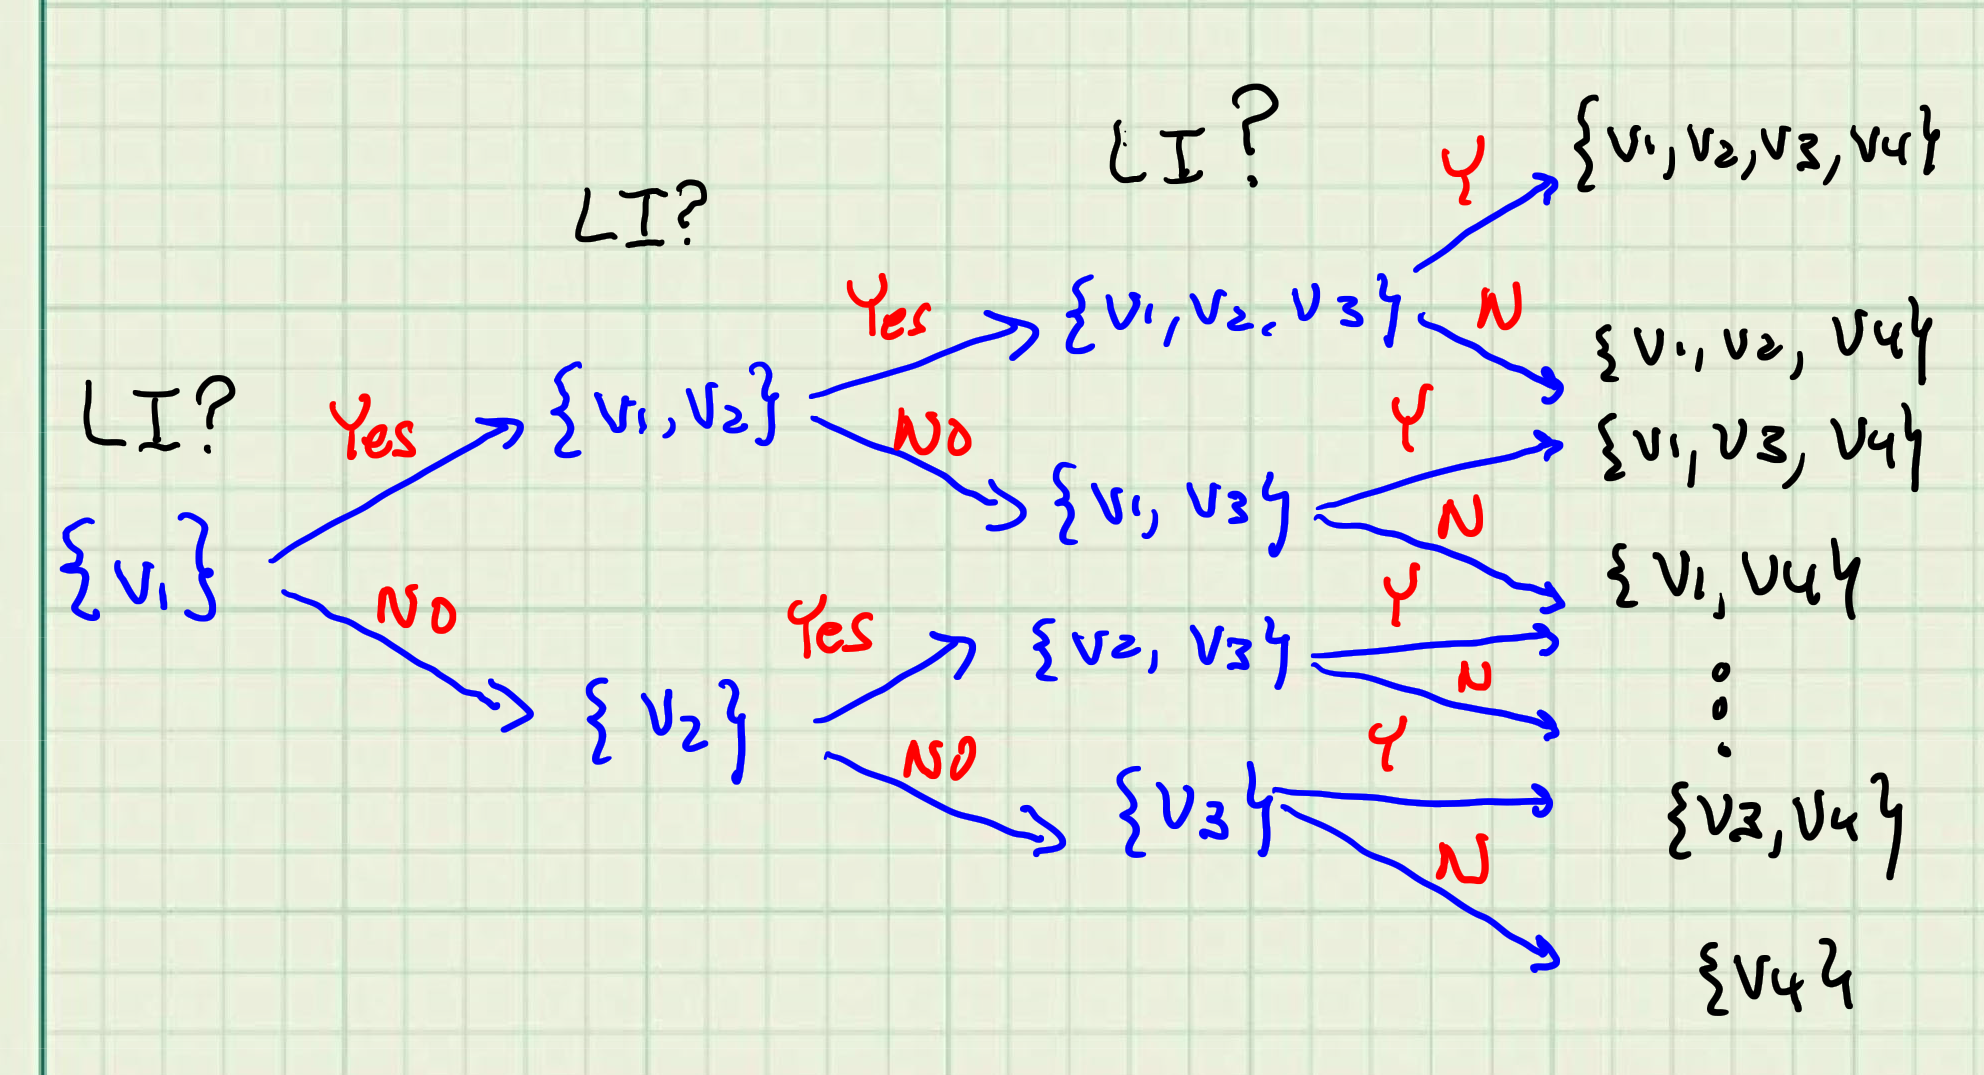
\includegraphics[width=0.88\columnwidth]{graphics/Chap05/NumberLinearIndependentVectorsInSet.png}
\caption[]{Checking linear independence from left to right. You could also start from the right and go to the left, or you could start in the middle and proceed to the two ends. You just need to do an organized search of the vectors!}
    \label{fig:NumberLinearlyIndependentVectors}
\end{figure}

In the following, we will implement the process indicated in Fig.~\ref{fig:NumberLinearlyIndependentVectors}, which shows one way to systematically check linear independence of a set of vectors to arrive at a maximal subset of linearly independent vectors. Along the way, we'll also keep track of the indices of the vectors that are linearly independent.\\ 

\begin{lstlisting}[language=Julia,style=mystyle]
function mySearchRoutine4NumIndepVectors(A,atol=1e-10)
    nRowsA, nColsA = size(A)
    V=Matrix{Float64}(undef, nRowsA, 0) # create an empty matrix
                                    # for storing independent vectors
    numIndVectors= 0
    indices = Vector{Int64}(undef, 0)  # create an empty vector for storing
                                # the indices of independent vectors
    for i = 1 : nColsA
        Temp=[V  A[:,i]]
        L, U, P = myLU(Temp'*Temp)
        minDiagU = minimum(abs.(diag(U)))
        # If minDiagU > atol, then U is invertible and hence the columns
        # of Temp are linearly independent
        if minDiagU > atol
            numIndVectors = numIndVectors + 1
            V = Temp
            indices = [indices; i] # keep track of indep vectors
        end
    end
    return numIndVectors, V, indices
end
\end{lstlisting}
\textbf{Output} 
\begin{verbatim}
mySearchRoutine4NumIndepVectors (generic function with 2 methods)
\end{verbatim}

We next show that $A$ has three linearly independent columns and we can choose them as the first, second, and fifth columns. \\

\begin{lstlisting}[language=Julia,style=mystyle]
numIndVectors, V, indices = mySearchRoutine4NumIndepVectors(A)
\end{lstlisting}
\textbf{Output} 
\begin{verbatim}
3, [0.8814395099307569 1.1974345124883454 -0.9375085811788099; -0.4241418472936163
1.1761409436174899 0.8276128787991263; … ; -0.15514669800915096 2.949627319800578
-0.1905215623370098; -1.2632013933716764 -0.10460087472162416 0.7201716618604121], 
[1, 2, 5])
\end{verbatim}

\begin{lstlisting}[language=Julia,style=mystyle]
numIndVectors
\end{lstlisting}
\textbf{Output} 
\begin{verbatim}
3
\end{verbatim}

\begin{lstlisting}[language=Julia,style=mystyle]
V
\end{lstlisting}
\textbf{Output} 
\begin{verbatim}
5×3 Matrix{Float64}:
  0.88144    1.19743   -0.937509
 -0.424142   1.17614    0.827613
  1.03061   -0.312031  -1.49514
 -0.155147   2.94963   -0.190522
 -1.2632    -0.104601   0.720172
\end{verbatim}

\begin{lstlisting}[language=Julia,style=mystyle]
indices
\end{lstlisting}
\textbf{Output} 
\begin{verbatim}
3-element Vector{Int64}:
 1
 2
 5
\end{verbatim}

Could we have made other choices for three linearly independent vectors? Absolutely. The following shows that we could have taken the last three vectors. 
\begin{lstlisting}[language=Julia,style=mystyle]
 numIndVectors, V, indices = mySearchRoutine4NumIndepVectors(A[:,3:5])
\end{lstlisting}
\textbf{Output} 
\begin{verbatim}
(3, [2.503340396444761 -1.8787774833565118 -0.9375085811788099; 2.1314687886946517
-3.5429649155470724 0.8276128787991263; … ; 5.576055157377987 -7.68964057029396
-0.1905215623370098; -0.5197147429767035 -1.3969985094856063 0.7201716618604121], 
[1, 2, 3])
\end{verbatim}

Could we have taken any three vectors? Let's check! We'll do a brute force search to find all combinations of three vectors that are linearly \textbf{dependent}, if any. Note that we can assume without loss of generality that $i < j < k$ when we consider three columns $\{A_i, A_j, A_k \}$ of $A$. Why? Because order does not change linear independence. \\

This code block outputs all combinations of three vectors that are linearly dependent.  \\

\begin{lstlisting}[language=Julia,style=mystyle]
for i = 1:3
    for j = i+1:5
        for k = j+1:5
             numIndVectors, V, indices = mySearchRoutine4NumIndepVectors(A[:,[i;j;k]])
            if numIndVectors < 3 
                @show [i;j;k]  # dependent columns              
            end
        end
    end
end
\end{lstlisting}
\textbf{Output}
\begin{verbatim}
[i; j; k] = [1, 2, 3]
[i; j; k] = [1, 2, 4]
[i; j; k] = [1, 3, 4]
[i; j; k] = [2, 3, 4]
\end{verbatim}

Once we know all combinations of columns of $A$ that are linearly dependent, we can deduce that the following sets of vectors are linearly independent.
\begin{itemize}
    \item  $\{A_1, A_2, A_5 \}$ 
    \item  $\{A_1, A_3, A_5 \}$ 
    \item  $\{A_2, A_3, A_5 \}$ 
    \item  $\{A_2, A_4, A_5 \}$ 
     \item  $\{A_3, A_4, A_5 \}$ 
\end{itemize}

\section{LDLT Factorization: A One-shot Means to Find Linearly Independent Vectors in a Set}

Once again, consider the vectors in $\real^n$,
$$\left\{v_1=\begin{bmatrix} a_{11} \\ a_{21}\\ \vdots \\ a_{n1} \end{bmatrix},  v_2=\begin{bmatrix} a_{12} \\ a_{22}\\ \vdots \\ a_{n2} \end{bmatrix}, ...,  v_m=\begin{bmatrix} a_{1m} \\ a_{2m}\\ \vdots \\ a_{nm} \end{bmatrix} \right\},$$ 
and use them as the columns of a matrix that we call $A$,
\begin{equation}
\label{eq:MatrixFromLinearIndependence_proTipC02}    
A=\left[\begin{array}{cccc} a_{11}& a_{12}& \cdots & a_{1m} \\
 a_{21}& a_{22}& \cdots & a_{2m}  \\
 \vdots & \vdots&  \ddots & \vdots \\
 a_{n1}& a_{n2}& \cdots & a_{nm} 
 \end{array}\right].
 \end{equation}

\begin{tcolorbox}[sharp corners, colback=green!30, colframe=green!80!blue,
title=\textbf{ {\Large \textcolor{red}{\bf Uber} Pro-Tip:} \large Number of Linearly Independent Vectors via an Enhanced LU Factorization}]
Assume that a set of vectors has been stacked to form the columns of an $n \times m$ matrix $A$ as in \eqref{eq:MatrixFromLinearIndependence_proTipC02}. \textbf{Fact:} The matrix $A^\top \cdot A$ always has an \textbf{LDLT Factorization}
\begin{equation}
    \label{eq:LDLTfactorization}
    P\cdot A^\top \cdot A \cdot P^\top = L\cdot D \cdot L^\top,
\end{equation}
where
\begin{itemize}
    \item $P$ is a (row) permutation matrix;
    \item $P^\top$, the transpose of $P$, permutes the columns of $A^\top A$;
    \item $L$ is uni-lower triangular and $L^\top$, the transpose of $L$, is therefore uni-upper triangular; and
    \item $D$ is diagonal and has non-negative entries.
\end{itemize}
\textcolor{red}{\bf Moreover,}
\begin{itemize}
    \item \textcolor{red}{\bf the number of linearly independent columns of $A$ is equal to the number of non-zero entries on the diagonal of $D$;} and, if we denote this number by $k$,
    \item  \textcolor{red}{\bf then for the version of the LDLT given below, the first $k$-columns of $A \cdot P^\top$ are linearly independent, and the remaining $(m-k)$-columns (if any) are linearly dependent on the first $k$ columns.} 
    \item Because the columns of $A\cdot P^\top$ are simply the columns of $A$ permuted by $P^\top$ (that is, re-ordered by the permutation matrix), \textcolor{red}{\bf the first $k$-columns of $A \cdot P^\top$ provide a selection of linearly independent columns of $A$}.
\end{itemize}

\end{tcolorbox}

While the derivation of this algorithm is not so different than what we did for the LU Factorization, we are still going to skip it. The main point is that matrices of the form $A^\top \cdot A$ always have an LDLT Factorization and, moreover, the diagonal of $D$ and the permutation matrix $P$ tell you everything you need to know about the linearly independent vectors that make up the columns of $A$. 

\begin{lstlisting}[language=Julia,style=mystyle]
function ldltROB101(A)
    epsilon = 1e-12
    M = A'*A
    n,m = size(A)
    Areduced = M
    L = Array{Float64,2}(undef,m,0)
    Id = zeros(m,m) + I
    P = Id    
    D=zeros(m,m)
    for i=1:m
        ii=argmax(diag(Areduced[i:m,i:m]))
        mrow=ii[1]+(i-1)
        if !(i==mrow)
            P[[i,mrow],:]=P[[mrow,i],:]
            Areduced[[i,mrow],:]=Areduced[[mrow,i],:]
            Areduced[:,[i,mrow]]=Areduced[:,[mrow,i]]
        end
        if (i>1)
            L[[i,mrow],:] = L[[mrow,i],:]
        end
        pivot=Areduced[i,i]
        if !isapprox(pivot,0,atol=epsilon)
            D[i,i]=pivot
            C=Areduced[:,i]/pivot
            L=[L C]
            Areduced=Areduced-(C*pivot*C')
        else
            L=[L Id[:,i:m]]
            break
        end
    end
    diagD=diag(D)
    return L,P,D,diagD
end
\end{lstlisting}
\textbf{Output} 
\begin{verbatim}
ldltROB101 (generic function with 1 method)
\end{verbatim}

We apply LDLT to the same $5 \times 5$ matrix we used before, namely
\begin{equation}
A:= \left[
\begin{array}{rrrrr}
0.8814 & 1.1974 & 2.5033 & -1.8788 & -0.9375 \\
-0.4241 & 1.1761 & 2.1315 & -3.5430 & 0.8276 \\
1.0306 & -0.3120 & -0.3325 & 2.1482 & -1.4951 \\
-0.1551 & 2.9496 & 5.5761 & -7.6896 & -0.1905 \\
-1.2632 & -0.1046 & -0.5197 & -1.3970 & 0.7202 \\
\end{array}
\right]
\end{equation} 

\begin{lstlisting}[language=Julia,style=mystyle]
L,P,D,diagD = ldltROB101(A)
@show diagD
D
\end{lstlisting}
\textbf{Output} 
\begin{verbatim}
diagD = [81.779373907533, 5.130204240478989, 0.7812212873817588, 0.0, 0.0]

5×5 Matrix{Float64}:
 81.7794  0.0     0.0       0.0  0.0
  0.0     5.1302  0.0       0.0  0.0
  0.0     0.0     0.781221  0.0  0.0
  0.0     0.0     0.0       0.0  0.0
  0.0     0.0     0.0       0.0  0.0
\end{verbatim}

We see immediately that we have three linearly independent vectors. Can we find easily a set of three columns of $A$ that are linearly independent? Yes. If we form $A \cdot P^\top$, the \textbf{Uber Pro-tip} tells us that then the first three columns will be linearly indepenent.  
\begin{lstlisting}[language=Julia,style=mystyle]
Abar=A*P'
\end{lstlisting}
\textbf{Output} 
\begin{verbatim}
5×5 Matrix{Float64}:
 -1.87878   2.50334   -0.937509   1.19743    0.88144
 -3.54296   2.13147    0.827613   1.17614   -0.424142
  2.14821  -0.332486  -1.49514   -0.312031   1.03061
 -7.68964   5.57606   -0.190522   2.94963   -0.155147
 -1.397    -0.519715   0.720172  -0.104601  -1.2632
\end{verbatim}

\begin{equation}
\overline{A}: = A \cdot P =\left[
\begin{array}{rrrrr}
-1.8788 & 2.5033 & -0.9375 & 1.1974 & 0.8814 \\
-3.5430 & 2.1315 & 0.8276 & 1.1761 & -0.4241 \\
2.1482 & -0.3325 & -1.4951 & -0.3120 & 1.0306 \\
-7.6896 & 5.5761 & -0.1905 & 2.9496 & -0.1551 \\
-1.3970 & -0.5197 & 0.7202 & -0.1046 & -1.2632 
\end{array}
\right]
\end{equation}

\begin{lstlisting}[language=Julia,style=mystyle]
numIndVectors, V, indices = myNumIndepVectors(Abar[:,1:3])
numIndVectors
\end{lstlisting}
\textbf{Output} 
\begin{verbatim}
3
\end{verbatim}

Which columns are they? From the permutation matrix, we can see that LDLT has selected the fourth, third, and fifth columns of $A$, $\{A_4, A_3, A_5 \}$. The order is not very important; it's a consequence of my implementation using the largest available pivot element at each pass of ``peeling the onion". \\

\begin{lstlisting}[language=Julia,style=mystyle]
P'
\end{lstlisting}
\textbf{Output} 
\begin{verbatim}
5×5 adjoint(::Matrix{Float64}) with eltype Float64:
 0.0  0.0  0.0  0.0  1.0
 0.0  0.0  0.0  1.0  0.0
 0.0  1.0  0.0  0.0  0.0
 1.0  0.0  0.0  0.0  0.0
 0.0  0.0  1.0  0.0  0.0
\end{verbatim}

Why this order? Once again, the way I wrote the LDLT algorithm, it permutes large elements on the diagonal of $A^\top \cdot A$ to the front.\\

Below is another version of a function to find the number of linear independent columns in a matrix, along with a specification of which columns to use.

\begin{lstlisting}[language=Julia,style=mystyle]
function myNumIndepVectors(A,myTol=1e-10)
    nRowsA, nColsA = size(A)
    V=Matrix{Float64}(undef, nRowsA, 0)
    L,P,D,diagD = ldltROB101(A)
    indicesLDLT=findall(x->x>myTol, diagD)
    numIndVectors = length(indicesLDLT)
    Ptrans = P'
    indices = Vector{Int64}(undef, numIndVectors)
    for i = 1:numIndVectors
            ind=argmax(Ptrans[:,i])
            indices[i]=ind[1] 
    end
    V=A[:,indices]
        
    return numIndVectors, V, indices
end
\end{lstlisting}
\textbf{Output} 
\begin{verbatim}
myNumIndepVectors (generic function with 2 methods)
\end{verbatim}


\begin{lstlisting}[language=Julia,style=mystyle]
numIndVectors, V, indices = myNumIndepVectors(A)
@show numIndVectors
@show indices
V
\end{lstlisting}
\textbf{Output} 
\begin{verbatim}
numIndVectors = 3
indices = [4, 3, 5]

5×3 Matrix{Float64}:
 -1.87878   2.50334   -0.937509
 -3.54296   2.13147    0.827613
  2.14821  -0.332486  -1.49514
 -7.68964   5.57606   -0.190522
 -1.397    -0.519715   0.720172
\end{verbatim}

\section{Debugging}

Here, we'll focus on the LU Function in Julia. Let's build a solver for $Ax=b$, when $A$ is square and invertible, and $A$ and $b$ have compatible sizes. We assume that the functions \texttt{forwardsub(L, b)} and \texttt{backwardsub(U, b)} have already been defined and error checked!\\

Let's include some packages and create some data.

\begin{lstlisting}[language=Julia,style=mystyle]
using LinearAlgebra
using Random
Random.seed!(2001)

A = randn(4,4)
b=randn(4,1);
\end{lstlisting}
\textbf{Output} 
Nothing due to the semicolon. We next write our first cut at a function to solve $Ax=b$



\begin{lstlisting}[language=Julia,style=mystyle]
function mySolver(A,b)
    L,U = lu(A)
    y =  forwardsub(L, b)
    x = backwardsub(U, y)
    return x
    return x
end      
\end{lstlisting}
\textbf{Output} 
\begin{verbatim}
mySolver (generic function with 1 method)
\end{verbatim}

We run our function and it seems to work because it does produce output!

\begin{lstlisting}[language=Julia,style=mystyle]
x =  mySolver(A,b)
\end{lstlisting}
\textbf{Output} 
\begin{verbatim}
4-element Vector{Float64}:
  0.2793805449608082
  2.6408473207373446
 -2.3464083290282343
 -0.7884784181920488
\end{verbatim}

About this time, you run one of our Friendly Checks and fail it. And you go, no way, my function works; it produces no errors. Look, I have actual output! So you post to Piazza, saying hey, I failed the Friendly Check! What's wrong with my code or with the Friendly Check itself? \\

\textcolor{blue}{\bf \large About this time of the semester, we start asking you to do some serious debugging yourself. So, let's do it.} \\

We first check if the solution is correct.

\begin{lstlisting}[language=Julia,style=mystyle]
norm(A*x-b)
\end{lstlisting}
\textbf{Output} 
\begin{verbatim}
1.5606151971175222
\end{verbatim}

Ooops! That is not close to zero. What's wrong? Well, on line 2 of your function, you called Julia's LU function with permutations! OH my gosh, you're right. Let's include the permutation matrix. So we do it.

\begin{lstlisting}[language=Julia,style=mystyle]
function mySolver(A,b)
    L,U, P = lu(A)
    y =  forwardsub(L, P*b)
    x = backwardsub(U, y)
    return x
    return x
end 
\end{lstlisting}
\textbf{Output} 
\begin{verbatim}
mySolver (generic function with 1 method)
\end{verbatim}

Everything looks good. We give it a whirl....and Julia is super unhappy. 

\begin{lstlisting}[language=Julia,style=mystyle]
x =  mySolver(A,b)
\end{lstlisting}
\textbf{Output} 
\begin{verbatim}
DimensionMismatch("matrix A has dimensions (4,1), matrix B has dimensions (4,1)")

Stacktrace:
  [1] _generic_matmatmul!(C::Matrix{Float64}, tA::Char, tB::Char, A::Matrix{Int64},
  B::Matrix{Float64}, _add::LinearAlgebra.MulAddMul{true, true, Bool, Bool})
    @ LinearAlgebra /buildworker/worker/package_linux64/build/usr/share/julia/stdlib/v1.6/
    LinearAlgebra/src/matmul.jl:814
  [2] generic_matmatmul!(C::Matrix{Float64}, tA::Char, tB::Char, A::Matrix{Int64}, 
  B::Matrix{Float64}, _add::LinearAlgebra.MulAddMul{true, true, Bool, Bool})
    @ LinearAlgebra /buildworker/worker/package_linux64/build/usr/share/julia/stdlib/
    v1.6/LinearAlgebra/src/matmul.jl:802
  [3] mul!
    @ /buildworker/worker/package_linux64/build/usr/share/julia/stdlib/
    v1.6/LinearAlgebra/src/matmul.jl:302 [inlined]
  [4] mul!
    @ /buildworker/worker/package_linux64/build/usr/share/julia/stdlib/
    v1.6/LinearAlgebra/src/matmul.jl:275 [inlined]
  [5] *
    @ /buildworker/worker/package_linux64/build/usr/share/julia/stdlib/
    v1.6/LinearAlgebra/src/matmul.jl:153 [inlined]
  [6] *
    @ /buildworker/worker/package_linux64/build/usr/share/julia/stdlib/
    v1.6/LinearAlgebra/src/matmul.jl:63 [inlined]
  [7] mySolver(A::Matrix{Float64}, b::Matrix{Float64})
    @ Main ./In[24]:3
  [8] top-level scope
    @ In[25]:1
  [9] eval
    @ ./boot.jl:360 [inlined]
 [10] include_string(mapexpr::typeof(REPL.softscope), mod::Module, 
 code::String, filename::String)
    @ Base ./loading.jl:1094
\end{verbatim}

We have a \textbf{DimensionMismatch("matrix A has dimensions (4,1), matrix B has dimensions (4,1)")} and it seems to be on line 3 of our function; we get that fron \texttt{@ Main ./In[14]:3}. So, we immediately suspect the function \texttt{backwardsub} has an error. However, we've used it many times before, and the line 
\begin{verbatim}
Stacktrace:
  [1] _generic_matmatmul!(C::Matrix{Float64}, tA::Char, tB::Char, A::Matrix{Int64}, 
  B::Matrix{Float64}, _add::LinearAlgebra.MulAddMul{true, true, Bool, Bool}) 
  \end{verbatim}
could tell us that we have a matrix multiplication problem. \\

Hence, let's use the \texttt{display} function to see what's up with that line of code. To save space here, we also include the function call on line 13. The output looks great, until it doesn't! 


\begin{lstlisting}[language=Julia,style=mystyle]
function mySolver(A,b)
    L,U,P = lu(A)
    display(L)
    display(U)
    display(P)
    display(P*b)
    y =  forwardsub(L, P*b)
    x = backwardsub(U, y)
    return x
    return x
end 

x =  mySolver(A,b)
\end{lstlisting}
\textbf{Output} 
\begin{verbatim}
4×4 Matrix{Float64}:
  1.0        0.0       0.0      0.0
 -0.374657   1.0       0.0      0.0
 -0.841164  -0.808034  1.0      0.0
 -0.207949  -0.591682  0.91447  1.0
4×4 Matrix{Float64}:
 -1.61455   0.810841   0.867077  -0.318762
  0.0      -1.66425   -0.958626  -1.56293
  0.0       0.0        0.811276  -1.17566
  0.0       0.0        0.0       -0.920034
4-element Vector{Int64}:
 1
 3
 4
 2
DimensionMismatch("matrix A has dimensions (4,1), matrix B has dimensions (4,1)")

Stacktrace:
  [1] _generic_matmatmul!(C::Matrix{Float64}, tA::Char, tB::Char, A::Matrix{Int64}, 
  B::Matrix{Float64}, _add::LinearAlgebra.MulAddMul{true, true, Bool, Bool})
    @ LinearAlgebra /buildworker/worker/package_linux64/build/usr/share/
    julia/stdlib/v1.6/LinearAlgebra/src/matmul.jl:814
  [2] generic_matmatmul!(C::Matrix{Float64}, tA::Char, tB::Char, A::Matrix{Int64}, 
  B::Matrix{Float64}, _add::LinearAlgebra.MulAddMul{true, true, Bool, Bool})
    @ LinearAlgebra /buildworker/worker/package_linux64/build/usr/share/julia/stdlib/
    v1.6/LinearAlgebra/src/matmul.jl:802
  [3] mul!
    @ /buildworker/worker/package_linux64/build/usr/share/julia/stdlib/
    v1.6/LinearAlgebra/src/matmul.jl:302 [inlined]
  [4] mul!
    @ /buildworker/worker/package_linux64/build/usr/share/julia/stdlib/
    v1.6/LinearAlgebra/src/matmul.jl:275 [inlined]
  [5] *
    @ /buildworker/worker/package_linux64/build/usr/share/julia/stdlib/v1.6/
    LinearAlgebra/src/matmul.jl:153 [inlined]
  [6] *
    @ /buildworker/worker/package_linux64/build/usr/share/julia/stdlib/
    v1.6/LinearAlgebra/src/matmul.jl:63 [inlined]
  [7] mySolver(A::Matrix{Float64}, b::Matrix{Float64})
    @ Main ./In[27]:6
  [8] top-level scope
    @ In[27]:13
  [9] eval
    @ ./boot.jl:360 [inlined]
 [10] include_string(mapexpr::typeof(REPL.softscope), mod::Module, 
 code::String, filename::String)
    @ Base ./loading.jl:1094

\end{verbatim}

From \texttt{\@ Main ./In[27]:6}, we see that we have an error on line 6. Also, looking at the displayed results, we note that the permutation matrix $P$ is a vector. Yikes! What is that all about? \textcolor{red}{\bf L,U, P = lu(A) returns, $L$, $U$, and the list of permutation indices, but not the permutation matrix.} \textbf{To obtain the matrix, you need to use }

\begin{lstlisting}[language=Julia,style=mystyle]
function mySolver(A,b)
    F = lu(A)
    U=F.U
    L=F.L
    P=F.P
    y =  forwardsub(L, P*b)
    x = backwardsub(U, y)
    return x
end 

x =  mySolver(A,b)
display(x)
norm(A*x- b)
\end{lstlisting}
\textbf{Output} 
\begin{verbatim}
4-element Vector{Float64}:
 -0.22542848860215622
 -2.222759959807066
  2.0136373165391372
  1.2566870405250985
  
7.2815418263566e-16
\end{verbatim}

\textbf{Bottom line:} We learned the following:
\begin{itemize}
    \item Just because a function runs with no errors does not mean it is correct. You, the creator of the function, need to run some simple tests to check the correctness of your function. Here, we simply applied the definition of $x$ being a solution to $Ax=b$, namely, $||Ax-b||=0$.

    \item There is useful information in the error messages. It takes practice to interpret them. At the very least, you can find the \textbf{line number} where things failed.

    \item Once you know approximately what is failing, insert a copious number of \texttt{display} or \texttt{@show} commands and compare what you see to what you expect. 

    \item Your checks can be much more focused than the generic Friendly Checks that we insert because you get to see where the error is occurring. 
\end{itemize}


\section{(Optional Read) Finding Counterexamples via Search}

How did we find a matrix where LU would mess up? We did a brute force search! 

\begin{lstlisting}[language=Julia,style=mystyle]
using LinearAlgebra
using Random
function CounterExample(atol=1e-10)
    # Set the seed because we want each student to obtain the same results
    Random.seed!(12121212)
    flag = 1
    N=5
    n=floor(Int,N/2)
    k=0
    while flag > 0
        # count how many times through the loop
        k=k+1
        Random.seed!(k)
        # Build a matrix A that has dependent column vectors
        B=randn(N,N-1)
        C=randn(n,n)
        A=[B[:,1:n] B[:,1:n]*C B[:,n+n:end]]
        # Apply LU to A'A
        F=lu(A'*A, check=false)
        diagU=diag(F.U)
        # Find all indices where the magnitue of the diagonal element is not too small
        indicesLU=findall(x->x>atol, abs.(diagU))
        # Now count them. This is LU's prediction of the number of linearly independent vectors
        NumLinIndepLU=length(indicesLU)
        # Apply LDLT to A'A; recall, our function forms A'*A
        L,P,D,diagD = ldltROB101(A)
         # Find all indices where the magnitue of the diagonal element is not too small
        indicesLDLT=findall(x->x>atol, diagD)
        # Now count them. This is LDLT's prediction of the number of linearly independent vectors
        NumLinIndepLDLT=length(indicesLDLT)
        # Check for a discrepancy in their reported number of linearly indep columns
        # and also, do not run forever. 1e5 seems like enough times to loop through random matrices
        if (NumLinIndepLDLT > NumLinIndepLU)||(k>1e5)
            return k, A, F, L, P, D, diagD
            flag=0
        end        
    end
end

function cleanUp(A,tol=1e-10)
    # Zero out small entries of a matrix or vector
    B=copy(A)
    indicesSmall=findall(x->x<tol, abs.(B))
    B[indicesSmall]=0.0*B[indicesSmall]
return B
end
\end{lstlisting}
\textbf{Output} 
\begin{verbatim}
CounterExample (generic function with 2 methods)
\end{verbatim}

\begin{lstlisting}[language=Julia,style=mystyle]
k, A, L, P, D, diagD = CounterExample()
println("It took us $k random matrices to generate an example where LU fails.")
println("Let's explore the example a bit.")
A
\end{lstlisting}
\textbf{Output} 
\begin{verbatim}
It took us 3 random matrices to generate an example where LU fails.

7×7 Matrix{Float64}:
  1.19156   -0.00197414  -0.51281   …  -1.06384    1.63691    0.633455
 -2.51973    1.00879     -1.58024       2.81498   -1.4239     0.68743
  2.07481    0.844223     0.511659     -3.14415    2.06393   -0.135094
 -0.97325    1.15807      0.733867     -0.118041  -1.31149    0.492822
 -0.101607  -0.475159    -1.40705       1.13615    0.756238   0.15671
 -1.54251   -0.244612    -0.707273  …   2.21941   -1.23019    1.23958
  0.100793   0.0718727   -1.1661        0.40164    0.923609  -1.21044
\end{verbatim}

% \begin{lstlisting}[language=Julia,style=mystyle]

% \end{lstlisting}
% \textbf{Output} 
% \begin{verbatim}

% \end{verbatim}

% \begin{lstlisting}[language=Julia,style=mystyle]

% \end{lstlisting}
% \textbf{Output} 
% \begin{verbatim}

% \end{verbatim}

% \begin{lstlisting}[language=Julia,style=mystyle]

% \end{lstlisting}
% \textbf{Output} 
% \begin{verbatim}

% \end{verbatim}

% \begin{lstlisting}[language=Julia,style=mystyle]

% \end{lstlisting}
% \textbf{Output} 
% \begin{verbatim}

% \end{verbatim}


% \begin{lstlisting}[language=Julia,style=mystyle]

% \end{lstlisting}
% \textbf{Output} 
% \begin{verbatim}

% \end{verbatim}

% \begin{lstlisting}[language=Julia,style=mystyle]

% \end{lstlisting}
% \textbf{Output} 
% \begin{verbatim}

% \end{verbatim}

% \begin{lstlisting}[language=Julia,style=mystyle]

% \end{lstlisting}
% \textbf{Output} 
% \begin{verbatim}

% \end{verbatim}

% \begin{lstlisting}[language=Julia,style=mystyle]

% \end{lstlisting}
% \textbf{Output} 
% \begin{verbatim}

% \end{verbatim}

% \begin{lstlisting}[language=Julia,style=mystyle]

% \end{lstlisting}
% \textbf{Output} 
% \begin{verbatim}

% \end{verbatim}

% \begin{lstlisting}[language=Julia,style=mystyle]

% \end{lstlisting}
% \textbf{Output} 
% \begin{verbatim}

% \end{verbatim}

% \begin{lstlisting}[language=Julia,style=mystyle]

% \end{lstlisting}
% \textbf{Output} 
% \begin{verbatim}

% \end{verbatim}

% \begin{lstlisting}[language=Julia,style=mystyle]

% \end{lstlisting}
% \textbf{Output} 
% \begin{verbatim}

% \end{verbatim}

\chapter{Julia Lab 6: Matrix Null Space and Linear Regression}
\label{chap:Lab6}
\section*{Learning Objectives}

\begin{itemize}
\item Null space of a matrix and relation to linear independence
\item  Regression
\item Debugging, or finding and fixing errors in your code
\end{itemize}

\section*{Outcomes} 
\begin{itemize}
\item A new way to check for linear independence
\item A brief introduction to basis vectors
\item Practice with a linear algebra Super Power, Linear Regression
\item Practice with ``broadcasting''
\item Practice with plotting
\item Knowledge that you can use linear regression to fit nonlinear functions to ``curved data''  as long as the unknown coefficients enter in a linear manner
\end{itemize}

\vspace*{1cm}

\textbf{Either download Lab6 from our Canvas site or open up a Jupyter notebook so that you can enter code as we go. It is suggested that you have line numbering toggled on.}  

\newpage

We've covered most of the Julia coding that we need for ROB 101. This lab will focus on the null space of a matrix and linear regression. 

\section{Null Space of a Matrix}

The null space of a matrix can be used to find linear combinations of vectors that add up to zero. Specifically, consider a set of vectors $\{ v_1, v_2, \ldots, v_m\} \subset \real^n$ and form the $n \times m$ matrix 
$$A = \left[ v_1 ~ v_2 ~\cdots ~v_m\right].$$ 
From lecture, the \textbf{null space of $A$} is 
$${\rm null}(A):=\{x \in \real^m~| ~ A x = 0_{n \times 1}   \}. $$
If $x \in {\rm null}(A)$ and $x \neq 0_{m \times 1} $, then we have a set of non-zero coefficients such 
$$x_1 v_1 + x_2 v_2 + \ldots + x_m v_m = 0_{n \times 1} $$
which means the set of vectors is \textbf{linearly dependent}. On the other hand, if the null space of $A$ consists only of the zero vector, then the set of vectors is \textbf{linearly independent}.

\begin{rem} If you do not like denoting the coefficients in the linear combination by $x_i$, then we can use $\alpha_i$ instead and write 
$$A \cdot \alpha = 0_{n \times 1} \iff \alpha_1 v_1 + \alpha_2 v_2 + \ldots + \alpha_m v_m = 0_{n \times 1}.$$
\end{rem}

\begin{lstlisting}[language=Julia,style=mystyle]
# The nullspace command in Julia LinearAlgebra package
using LinearAlgebra

A = [1 2 3 4; 5 6 7 8; 9 10 11 12]
V = nullspace(A)
\end{lstlisting}
\textbf{Output} 
\begin{verbatim}
4×2 Matrix{Float64}:
  0.261535  -0.481248
 -0.707414   0.446727
  0.630224   0.550289
 -0.184345  -0.51576
\end{verbatim}

\begin{lstlisting}[language=Julia,style=mystyle]
v1 = V[:,1]
v2 = V[:,2]
@show A*v1 # needs to be zero for v1 to be in the null space
@show A*v2 # similar. 
\end{lstlisting}
\textbf{Output} 
\begin{verbatim}
A * v1 = [-1.1102230246251565e-16, 2.220446049250313e-16, 2.220446049250313e-15]
A * v2 = [0.0, -8.881784197001252e-16, -8.881784197001252e-16]

3-element Vector{Float64}:
  0.0
 -8.881784197001252e-16
 -8.881784197001252e-16
\end{verbatim}

We check that vectors in the null space tell us how to form linear combinations of the columns of $A$ that add up to zero. \\

\begin{lstlisting}[language=Julia,style=mystyle]
# Linear combination of the columns of A that adds up to zero
a1=V[1,1]
a2=V[2,1]
a3=V[3,1]
a4=V[4,1]
#
a1*A[:,1] + a2*A[:,2] + a3*A[:,3] + a4*A[:,4]
\end{lstlisting}
\textbf{Output} 
\begin{verbatim}
3-element Vector{Float64}:
 -1.1102230246251565e-16
  2.220446049250313e-16
  2.220446049250313e-15
\end{verbatim}

\begin{lstlisting}[language=Julia,style=mystyle]
# Linear combination of the columns of A that adds up to zero
a1=V[1,2]
a2=V[2,2]
a3=V[3,2]
a4=V[4,2]
#
a1*A[:,1] + a2*A[:,2] + a3*A[:,3] + a4*A[:,4]
\end{lstlisting}
\textbf{Output} 
\begin{verbatim}
3-element Vector{Float64}:
  0.0
 -8.881784197001252e-16
 -8.881784197001252e-16
\end{verbatim}

We also recall from lecture that the null space of a matrix is a subspace. Indeed, $v_i \nullspace(A) \iff A v_1 = 0_{n \times 1}$, and thus, if we consider a linear combination of vectors in the null space of $A$, and apply $A$ to it, we get the zero vector. Indeed, 
$$A \cdot(\alpha_1 v_1 + \alpha_2 v_2) = \alpha_1 A \cdot v_1 + \alpha_2 A \cdot v_2 = \alpha_1 0_{n \times 1} + \alpha_2 0_{n \times 1}  =  0_{n \times 1}.$$
So, if a null space is a subspace, why is the command \texttt{nullspace} only returning two vectors? \\

\begin{lstlisting}[language=Julia,style=mystyle]
# The nullspace command in Julia LinearAlgebra package
using LinearAlgebra

A = [1 2 3 4; 5 6 7 8; 9 10 11 12]
println("If a null space is a subspace, why is the command only returning two vectors?")
V = nullspace(A)
\end{lstlisting}
\textbf{Output} 
\begin{verbatim}
If a null space is a subspace, why is the command only returning two vectors?

4×2 Matrix{Float64}:
  0.261535  -0.481248
 -0.707414   0.446727
  0.630224   0.550289
 -0.184345  -0.51576
\end{verbatim}

The \texttt{nullspace} command in Julia is returning a ``basis'' for the subspace. When you are first reading this, we may not have covered the concept of basis vectors in lecture. Hence, we give a preview of the definition here.


\begin{tcolorbox}[title=\textbf{Preview of Basis Vectors}] We are delaying the formal study of basis vectors until Chapter~10 in our textbook. In the meantime, it helps to have an intuitive understanding:
\begin{itemize}
    \item A set of vectors $\{ v_1, v_2,  \ldots, v_m\} \subset V$ is a \textbf{basis for $V$} if
    \begin{enumerate}
    \renewcommand{\labelenumi}{(\alph{enumi})}
\setlength{\itemsep}{.2cm}
        \item $\{ v_1, v_2,  \ldots, v_m\}$ is linearly independent
        \item $x\in V \iff$ there exist coefficients $\alpha_1, \ldots, \alpha_m$ such that $x = \alpha_1 v_1  + \cdots + \alpha_m v_m$.
    \end{enumerate}
\item Personally, your instructor likes to think of a basis $\{ v_1, v_2,  \ldots, v_m\} \subset V$ in the following way:
\begin{enumerate}
    \renewcommand{\labelenumi}{(\alph{enumi})}
\setlength{\itemsep}{.2cm}
    \item  The set $\{ v_1, v_2,  \ldots, v_m\}$  is \textbf{big enough to generate $V$ by forming linear combinations}, and
    \item \textbf{small enough to be linearly independent}.
    \end{enumerate}
\end{itemize}
 
\end{tcolorbox}

\vspace*{.2cm}

\textbf{A Goldilocks interpretation of a basis for a subspace $V$}: \textcolor{red}{\bf a basis is a set of vectors that is not too big and not too small.} 
\begin{itemize}

    \item If every $x \in V$ can be expressed as a linear combination of elements of $\{ v_1, v_2,  \ldots, v_m\}$, then  $\{ v_1, v_2,  \ldots, v_m\}$ is \textbf{big enough} to ``generate'' all of $V$. 
        \item If the set  $\{ v_1, v_2,  \ldots, v_m\}$ is linearly independent, then it is \textbf{small enough} that you cannot discard elements without changing the number of linearly independent vectors.
        \item Hence, a basis is \textbf{``just right''} in terms of the quantity of vectors you need to build every vector in the subspace through the operation of forming linear combinations.
\end{itemize}

\vspace*{.2cm}

\begin{tcolorbox}[title=\textbf{Another Test for Linear Independence}] Consider a set of vectors in $\real^n$,
$$\left\{v_1=\begin{bmatrix} a_{11} \\ a_{21}\\ \vdots \\ a_{n1} \end{bmatrix},  v_2=\begin{bmatrix} a_{12} \\ a_{22}\\ \vdots \\ a_{n2} \end{bmatrix}, ...,  v_m=\begin{bmatrix} a_{1m} \\ a_{2m}\\ \vdots \\ a_{nm} \end{bmatrix} \right\},$$ 
and use them as the columns of a matrix that we call $A$,
\begin{equation}
\label{eq:MatrixFromLinearIndependence_proTipCC}    
A=\left[\begin{array}{cccc} a_{11}& a_{12}& \cdots & a_{1m} \\
 a_{21}& a_{22}& \cdots & a_{2m}  \\
 \vdots & \vdots&  \ddots & \vdots \\
 a_{n1}& a_{n2}& \cdots & a_{nm} 
 \end{array}\right].
 \end{equation}
 The following statements are equivalent:
 \begin{itemize}
     \item  The set of vectors $ \{v_1, v_2, \ldots, v_m \} $ is linearly independent.
     \item The null space of $A$ is the zero vector, that is, the only vector $x\in \real^m$ satisfying $Ax = 0_{n \times 1}$ is the vector $x = 0_{m \times 1}$
 \end{itemize}
\end{tcolorbox}

\vspace*{.2cm}

Determine if the set of vectors $\{v_1, v_2, v_3, v_4\}$ is linearly independent or not. 
\begin{lstlisting}[language=Julia,style=mystyle]
using Random
Random.seed!(2021)
v1=randn(5,1)
v2=randn(5,1)
v3=randn(5,1)
v4=randn(5,1)

# Place your code below
A = [v1 v2 v3 v4]
println("Note how Julia reports that there are no non-zero vectors satisfying Ax = 0")
V = nullspace(A)
\end{lstlisting}
\textbf{Output} 
\begin{verbatim}
Note how Julia reports that there are no non-zero vectors satisfying Ax = 0

4×0 Matrix{Float64}
\end{verbatim}

\vspace*{.2cm}

Julia reported an ``empty basis''... there are no non-zero vectors required to generate the null space of $A$.\\

 Determine if the set of vectors $\{v_1, v_2, ..., v_6\}$ is linearly independent or not. If they are linearly dependent, find a set of not all identically zero coefficients such that $\alpha_1 v_1 + \alpha_2 v_2 + \cdots + \alpha_6 v_6= 0$. In other words, find a non-trivial linear combination of the set of vectors that adds up to the zero vector.\\

\begin{lstlisting}[language=Julia,style=mystyle]
using Random
Random.seed!(2021)
v1=randn(4,1)
v2=randn(4,1)
v3=randn(4,1)
v4=randn(4,1)
v5=randn(4,1)
v6=randn(4,1)

# Place your code below
# Compute alpha = [alpha1; alpha2; ...; alpha6]
# such that alpha1*v1 + alpha2*v2 + ... + alpha6*v6 = 0
# your code here
A = [v1 v2 v3 v4 v5 v6]
V = nullspace(A)
\end{lstlisting}
\textbf{Output} 
\begin{verbatim}
6×2 Matrix{Float64}:
 -0.884195    0.175427
 -0.0530824   0.686466
 -0.254579    0.093228
 -0.274888   -0.461607
  0.158941   -0.150481
  0.223037    0.50356
\end{verbatim}

\vspace*{.2cm}

\begin{lstlisting}[language=Julia,style=mystyle]
# solution continued
alpha = sqrt(3)*V[:,1] + pi*V[:,2]
\end{lstlisting}
\textbf{Output} 
\begin{verbatim}
6-element Vector{Float64}:
 -0.9803501037910766
  2.064655155074321
 -0.14805907841326366
 -1.926298965466871
 -0.19745609676639247
  1.9682934386167301
\end{verbatim}

\vspace*{.2cm}

\begin{lstlisting}[language=Julia,style=mystyle]
A*alpha
\end{lstlisting}
\textbf{Output} 
\begin{verbatim}
4-element Vector{Float64}:
  4.996003610813204e-16
  0.0
 -8.881784197001252e-16
  0.0
\end{verbatim}

%\vspace*{.2cm}

\section{Linear Regression or Least Squares Fit to Data}
\label{sec:LinearRegression}

We seek to fit a function to data. For example, we have a scatter plot of data points and wish to approximate the points with a straight line or perhaps a polynomial. It is assumed that you have scanned Chapter 8 in our textbook (not the Lab Manual).\\

% \begin{figure}[htb]%
% 	\centering
% 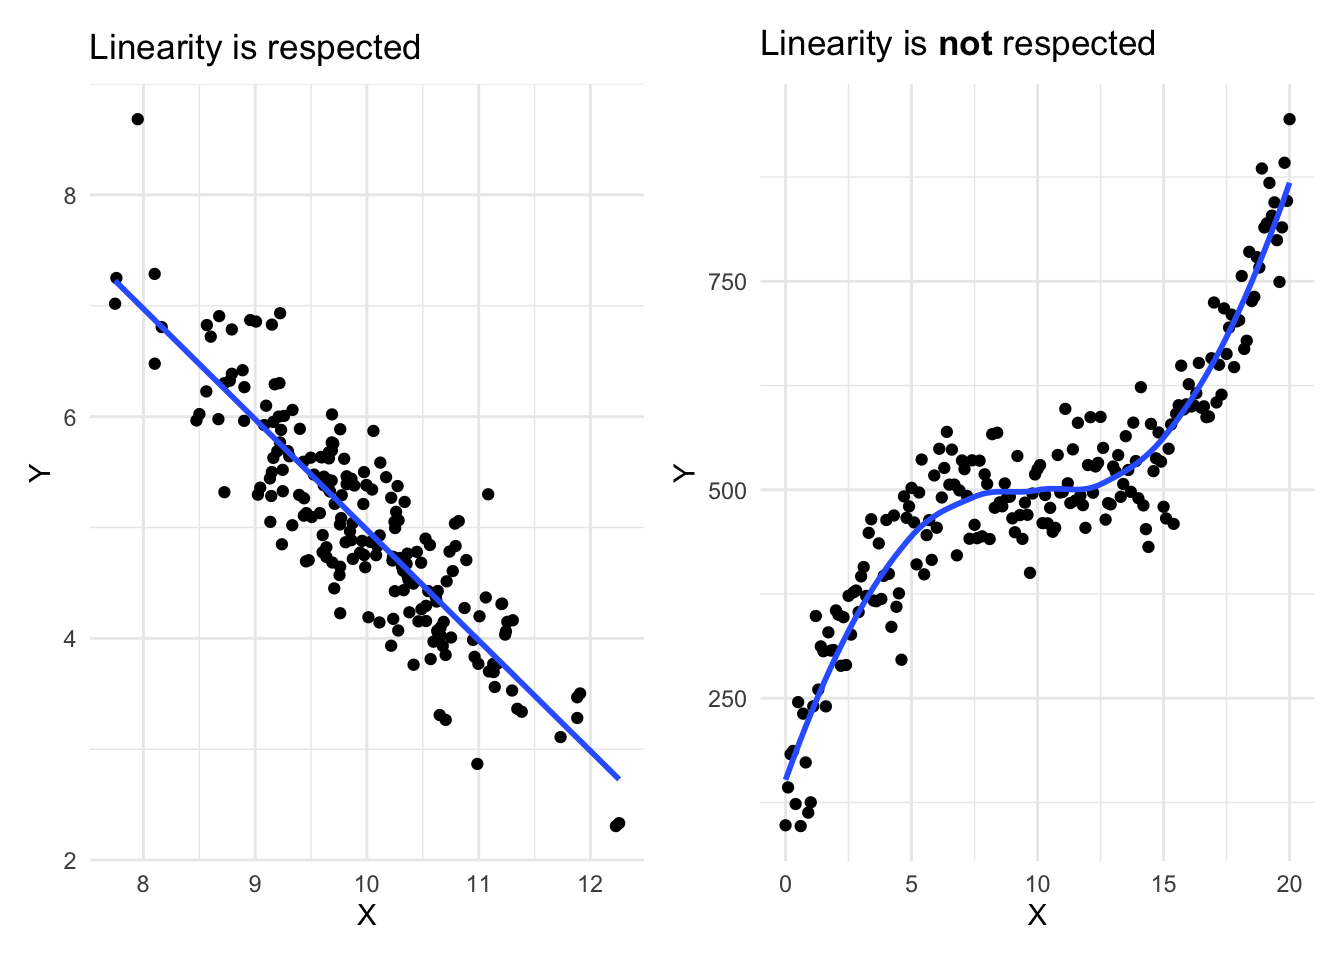
\includegraphics[width=0.6\columnwidth]{graphics/Chap06/Regression.png}
% \caption[]{From \url{https://www.r-bloggers.com/2021/10/multiple-linear-regression-made-simple/}. The first step is to plot your data and decide if you are fitting a line or something more complicated. As we will see, both can be accommodated via linear regression.}
%     \label{fig:Regression}
% \end{figure}

 The first step is to plot our data and decide if we are fitting a line or something more complicated. As we will see, both can be accommodated via linear regression.

\begin{lstlisting}[language=Julia,style=mystyle]
# Generate some points for line fitting
# Run me, don't change me. 
using Random
Random.seed!(2021)
NumPts = 100
m = 2
b = 1
x = -1 .+ 2*rand(NumPts,1)
y = m*x .+ b + 0.30*randn(NumPts, 1)

using Plots
scatter(x, y, legend=false)
\end{lstlisting}
\textbf{Output} 

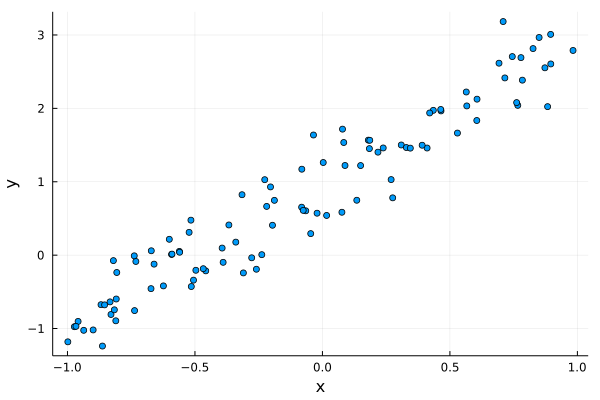
\includegraphics[width=0.6\columnwidth]{graphics/Chap06/LinearScatterPlot.png}

This looks appropriate for fitting a line. Hence, we assume a linear model ${y}=mx+b$. We set up the linear equations
$$y_i = b + m x_i  = \begin{bmatrix}  1 & x_i  \end{bmatrix} \begin{bmatrix} b \\ m \end{bmatrix},  ~~1 \le i \le N,$$ 
where $N$ is the number of data points (100 in our case), and write it out in matrix form
\begin{equation}
    \label{eq:FirstRegressionModel02}
\underbrace{\begin{bmatrix} y_1 \\ y_2 \\ \vdots \\y_N \end{bmatrix}}_{Y} = \underbrace{\left[\begin{array}{cc}
 1 &   x_1\\
  1 &     x_2  \\
  1 &     \vdots  \\
   1 &    x_N 
\end{array}  \right]}_{\Phi} \cdot  \underbrace{\begin{bmatrix} b \\ m \end{bmatrix}}_{\alpha},
\end{equation}
where $Y$ is the vector of $y$-data, $\Phi$ is called the \textbf{regressor matrix} and $\alpha$ is the vector of \textbf{unknown coefficients} that parameterize the  model.
\begin{lstlisting}[language=Julia,style=mystyle]
# Create the Y and the regressor matrix Phi
# Run me, don't change me.
Y = y
Phi = [ones(NumPts,1) x]
\end{lstlisting}
\textbf{Abridged Output} 
\begin{verbatim}
100×2 Matrix{Float64}:
 1.0  -0.188407
 1.0  -0.868452
 1.0  -0.203676
 1.0  -0.672369
 1.0   0.566187
 1.0  -0.731769
 .
 .
 .
 1.0   0.39111
 1.0  -0.0753372
 1.0   0.149722
 1.0  -0.816126
 1.0   0.420627
\end{verbatim}

\begin{tcolorbox}[title=\textbf{\large Least Squares Fit to Data also called Linear Regression}]

 From our textbook, if the columns of $\Phi$ are linearly independent, or equivalently, $\Phi^\top \Phi$ is invertible, then the following are equivalent 
  \begin{equation}
    \label{eq:ThmLeastSqaredErrorSolution2}
  \alpha^\ast = \left( \Phi^\top \Phi \right)^{-1}\Phi^\top Y  \iff  \alpha^\ast = \argmin_{\alpha} ||Y-\Phi \alpha ||^2 \iff \left( \Phi^\top \Phi \right) \alpha^\ast = \Phi^\top Y.
\end{equation}
  
  \end{tcolorbox}


\begin{lstlisting}[language=Julia,style=mystyle]
# OK for small problems, such as here, with two unknowns
A=Phi'*Phi
b=Phi'*Y
alpha = inv(A)*b
\end{lstlisting}
\textbf{Output} 
\begin{verbatim}
2×1 Matrix{Float64}:
 0.9472834926740609
 1.9393293464390031
\end{verbatim}


\begin{lstlisting}[language=Julia,style=mystyle]
scatter(x, y, legend=false)
y_hat = Phi * alpha
scatter!(x, y_hat)
titre="Regressed Line in Brown"
plot!(xlabel = "x", ylabel = "y", title=titre)
\end{lstlisting}
\textbf{Output} 

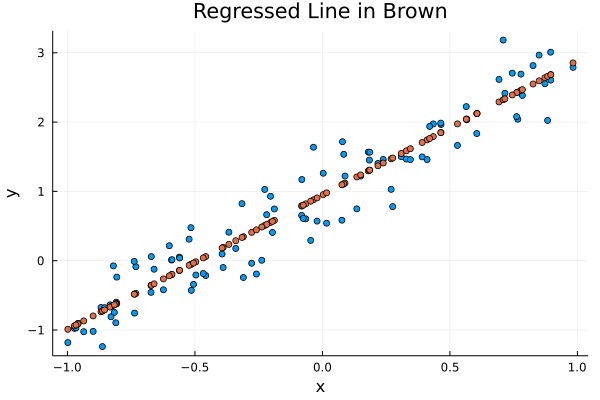
\includegraphics[width=0.6\columnwidth]{graphics/Chap06/LinearScatterPlotOverlay.png}

\begin{lstlisting}[language=Julia,style=mystyle]
# Generate some data for polynomial curve fitting
# Run me, don't change me.
#
using Random
Random.seed!(123456789)
NumPts = 100
x = -1 .+ 3*rand(NumPts,1)
a0 = 3
a1 = 6
a2 = 4
a3 = 6
a4 = -11
a5 = 2
a6 = -.2
# note the sin(2x) term
y = a6*x.^6 + a5*x.^5 + a4*x.^4 + a3*x.^3 + 
       a2*x.^2 .+ a1*sin.(2*x) .+ a0 + 1.50*randn(NumPts, 1)

using Plots
scatter(x,y,legend=false)
#png("PolyScatterPlot")
\end{lstlisting}
\textbf{Output} 

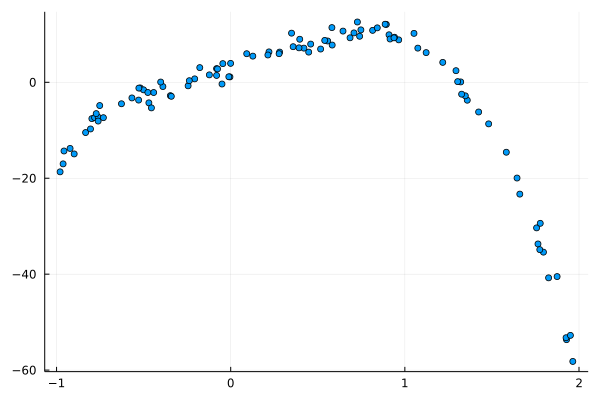
\includegraphics[width=0.7\columnwidth]{graphics/Chap06/PolyScatterPlot.png}



\begin{tcolorbox}[sharp corners, colback=green!30, colframe=green!80!blue, title=\textbf{\Large Large Scale Least Squares via the LU Factorization}]
 From our textbook,  if the columns of $\Phi$ are linearly independent, or equivalently, $\Phi^\top \Phi$ is invertible, we know the following are equivalent 
  \begin{equation}
    \label{eq:ThmLeastSqaredErrorSolution2secondTime}
  \alpha^\ast = \left( \Phi^\top \Phi \right)^{-1}\Phi^\top Y  \iff  \alpha^\ast = \argmin_{\alpha} ||Y-\Phi \alpha ||^2 \iff \left( \Phi^\top \Phi \right) \alpha^\ast = \Phi^\top Y.
\end{equation}
The suggested ``pipeline'' for  computing a least squared error solution to $ \left( \Phi^\top \Phi \right) \alpha^\ast = \Phi^\top Y$ is 
\begin{itemize}
    \item factor $P \cdot \left( \Phi^\top \Phi \right)  =: L \cdot U$, that is, do the LU Factorization of $\Phi^\top \cdot \Phi$,
    \item compute $\overline{b}:= P \cdot \Phi^\top Y$, and then 
    \item solve $L y = \overline{b}$ via forward substitution, and
    \item solve $U \alpha^\ast =y$ via backward substitution.
\end{itemize}
\end{tcolorbox}

\begin{lstlisting}[language=Julia,style=mystyle]
# Run me, don't change me. I am providing some nice functions for you.
# Forward and Back substitution functions from HW04

# This is a back substitution function.  It solves for x in an equation Ux = b, 
# where U is upper triangular. The function assumes U and b are the correct 
# sizes. You can add error checking, if you wish.
function backwardsub(U, b)
    # Check if U is non-signular
    min_diagU = minimum(abs.(diag(U)))
    if min_diagU <  1E-10
        return false
    end
    n = length(b)
    x = Vector{Float64}(undef, n) 
    x[n] = b[n]/U[n,n]
    for i in n-1:-1:1
        x[i]=(b[i]- (U[i,(i+1):n])' *x[(i+1):n] )./U[i,i]
    end
    return x
end
# This is a forward substitution function. It solves for x in an equation Lx = b, 
# where L is lower triangular. # The function assumes L and b are the correct 
# sizes. You can add error checking, if you wish.
function forwardsub(L, b)
     # Check if L is non-signular
    min_diagL = minimum(abs.(diag(L)))
    if min_diagL <  1E-10
        return false
    end
    n = length(b)
    x = Vector{Float64}(undef, n); 
    x[1] = b[1]/L[1,1] 
    for i = 2:n 
        x[i]=(b[i]- (L[i,1:i-1])' *x[1:i-1] )./L[i,i] 
    end
    return x
end
\end{lstlisting}
\textbf{Output} 
\begin{verbatim}
forwardsub (generic function with 1 method)
\end{verbatim}

\begin{lstlisting}[language=Julia,style=mystyle]
# Create the Y and the regressor matrix Phi
# Run me, don't change me.
Y = y
Phi = [ones(NumPts,1) x x.^2 x.^3 x.^4]
\end{lstlisting}
\textbf{Abridged Output} 
\begin{verbatim}
100×5 Matrix{Float64}:
 1.0   0.0919935   0.0084628    0.000778522   7.16189e-5
 1.0   0.90899     0.826264     0.751066      0.682712
 1.0   1.12227     1.25948      1.41347       1.58629
 1.0   1.58257     2.50452      3.96357       6.27261
 1.0   0.74038     0.548163     0.405849      0.300483
 1.0  -0.797207    0.63554     -0.506657      0.403911
 1.0  -0.206817    0.0427734   -0.00884629    0.00182957
 1.0  -0.177557    0.0315266   -0.00559777    0.000993924
 1.0   0.815018    0.664255     0.54138       0.441234
.
.
.
 1.0  -0.402096    0.161681    -0.0650113     0.0261408
 1.0   0.396441    0.157166     0.0623069     0.024701
 1.0  -0.0500005   0.00250005  -0.000125003   6.25023e-6
 1.0   0.685263    0.469585     0.321789      0.22051
 1.0  -0.898753    0.807756    -0.725973      0.65247
 1.0  -0.805068    0.648134    -0.521792      0.420078
\end{verbatim}


\begin{lstlisting}[language=Julia,style=mystyle]
# Find alpha by solving Phi' * Y= Phi' * Phi*alpha (Ax = b) using LU decomposition
using LinearAlgebra
F = lu(Phi' * Phi)
L = F.L
U = F.U
P = F.P
#
# Phi' * Y = Phi' * Phi * alpha
# after LU Factorization of Phi'*Phi, we have
# P *  Phi' * Y  = L * U * alpha
# 
y_alpha = forwardsub(L, P*Phi'*Y)
alpha = backwardsub(U, y_alpha)
\end{lstlisting}
\textbf{Output} 
\begin{verbatim}
5-element Vector{Float64}:
  3.71155035678547
 11.770104292873295
 -2.1786034505443537
  0.488282866753122
 -5.371244500774466
\end{verbatim}

\begin{lstlisting}[language=Julia,style=mystyle]
scatter(x, y, legend=false)
y_hat = Phi * alpha
scatter!(x, y_hat)
titre="Regressed Polynomial in Brown"
plot!(xlabel = "x", ylabel = "y", title=titre)
\end{lstlisting}
\textbf{Output} 


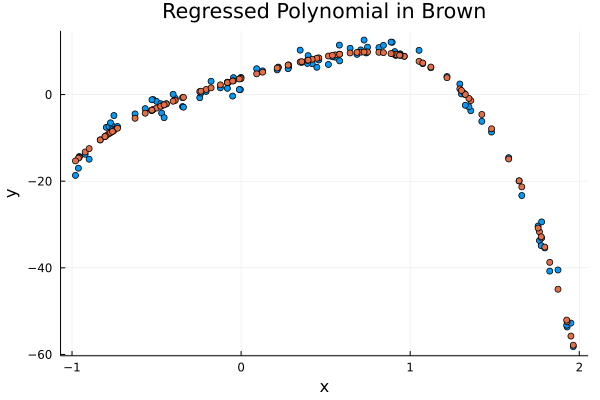
\includegraphics[width=0.7\columnwidth]{graphics/Chap06/PolyScatterPlotOverlay.png}

\section{Debugging}

Let's build a function \texttt{function LeastSquares\_Solve(Phi, Y)} that takes in a regressor matrix and a set of measurements, and returns the optimal parameters and data related to the quality of the fit. Because least squares fitting relies on solving $Ax=b$ when $A$ is square and invertible, we'll begin by building a function to compute exact solutions to square systems of linear equations. Moreover, we will build the function step-by-step and check for bugs as we go.\\
%%\label{sec:LinearRegression}

We start with baby steps. We only test for $A$ being square.
\begin{lstlisting}[language=Julia,style=mystyle]
# Function for solving Ax=b using LU decomposition
function Exact_Solve(A,b)
    nRows, nCols = size(A) 
    # We'll check for A not square. We assume A is a matrix.
    if ( nRows !== nCols)
         println("System of equations not properly formed")
        return x = NaN
    end
    xDummy= [1;2.0]
    return xDummy
end

A=[1 2; 3 4; 5 6]
b=[8; 9.0]
xAns = Exact_Solve(A,b)
\end{lstlisting}
\textbf{Output} 
\begin{verbatim}
System of equations not properly formed
NaN
\end{verbatim}
Next we add in a check that $b$ has the same number of rows as $A$. The command \texttt{||} ``double-pipes'' serves as the \texttt{logical or} command. We test it on good data and bad data. 

\begin{lstlisting}[language=Julia,style=mystyle]
# Function for solving Ax=b using LU decomposition
function Exact_Solve(A,b)
    nRows, nCols = size(A) 
    # We'll check for A not square. We assume A is a matrix.
    if ( nRows !== nCols)||(length(b) !== nRows)
         println("System of equations not properly formed")
        return x = NaN
    end
    xDummy= [1;2.0]
    return xDummy
end

A=[1 2; 3 4]
b=[8; 9.0; 11]
@show xAns = Exact_Solve(A,b)
b=[11, 13]
@show xAns = Exact_Solve(A,b);
\end{lstlisting}
\textbf{Output} 
\begin{verbatim}
System of equations not properly formed
xAns = Exact_Solve(A, b) = NaN
xAns = Exact_Solve(A, b) = [1.0, 2.0]
\end{verbatim}

Next we add in a solver via our beloved LU pipeline. We also check that the result is a valid solution of the equations.


\begin{lstlisting}[language=Julia,style=mystyle]
# Function for solving Ax=b using LU decomposition
function Exact_Solve(A,b)
    nRows, nCols = size(A) 
    # We'll check for A not square. We assume A is a matrix.
    if ( nRows !== nCols)||(length(b) !== nRows)
         println("System of equations not properly formed")
        return x = NaN
    end
    F=lu(A)
    y=forwardsub(F.L,F.P*b)
    x=backwardsub(F.U, y)
    return x
end

A=[1 2; 3 4]
b=[8; 9.0; 11]
@show xAns = Exact_Solve(A,b)
b=[11, 13]
@show xAns = Exact_Solve(A,b);
norm(A*xAns-b)
\end{lstlisting}
\textbf{Output} 
\begin{verbatim}
System of equations not properly formed
xAns = Exact_Solve(A, b) = NaN
xAns = Exact_Solve(A, b) = [-9.0, 10.0]

0.0
\end{verbatim}
We now add a tolerance and check for $A$ being singular. If $A$ is singular, we return \texttt{x=NaN}; otherwise, we implement the LU pipeline. We are very proud of our function!

\begin{lstlisting}[language=Julia,style=mystyle]
# Function for solving Ax=b using LU decomposition
function Exact_Solve(A,b,aTol=1e-10)
    nRows, nCols = size(A)
    if (length(b) !== nRows)||( nRows !== nCols)
         println("System of equations not properly formed")
        return x=NaN
    end
    F=lu(A)
    if minimum(abs.(diag(F.U))) < aTol
        println("diagU has numbers that are nearly zero")
        return x=NaN
    else
        y=forwardsub(F.L,F.P*b)
        x=backwardsub(F.U, y)
        return x 
    end
end

A=[1 1; 0 1e-14]
b=[8; 9.0]
@show xAns = Exact_Solve(A,b)
#
A=[1 1; 3 4]
b=[11, 13]
@show xAns = Exact_Solve(A,b)
norm(A*xAns-b)
\end{lstlisting}
\textbf{Output} 
\begin{verbatim}
diagU has numbers that are nearly zero
xAns = Exact_Solve(A, b) = NaN
xAns = Exact_Solve(A, b) = [31.00000000000001, -20.000000000000007]

3.552713678800501e-15
\end{verbatim}

Now we do a real life-size check! 

\begin{lstlisting}[language=Julia,style=mystyle]
using Random
A = randn(1000,1000)
b=randn(1000,1)
xAns = Exact_Solve(A,b);
norm(A*xAns-b)
\end{lstlisting}
\textbf{Output} 
\begin{verbatim}
2.643871993979311e-11
\end{verbatim}

And it looks great! So next, we develop a least squares solver. We use the fact that \texttt{alphaStar} satisfies
$$ \Phi^\top Y = \Phi^\top \cdot \Phi \alpha^\ast \iff \Phi^\top \cdot \Phi \alpha^\ast = \Phi^\top Y $$
and thus \texttt{alphaStar} should be the exact solution to $Ax=b$, for 
$$A \longleftrightarrow\Phi^\top \cdot \Phi , b\longleftrightarrow \Phi^\top Y, x \longleftrightarrow \alpha^\ast. $$


\begin{lstlisting}[language=Julia,style=mystyle]
# Function for fitting data with Least Squares
function LeastSquares_Solve(Phi, Y)
    alphaStar = Exact_Solve(Phi'*Phi, Phi'*Y) # Phi'*Y = Phi'*Phi * alpha
    # Return some extra quantities
    Yhat = Phi*alphaStar
    Error = Y-Yhat
    SqError = Error'*Error
    RootMeanSqError = sqrt(SqError/length(Y))
    return alphaStar, Yhat, RootMeanSqError
end
\end{lstlisting}
\textbf{Output} 
\begin{verbatim}
LeastSquares_Solve (generic function with 1 method)
\end{verbatim}

Now we run a real test!

\begin{lstlisting}[language=Julia,style=mystyle]
# Generate some data for polynomial curve fitting
# Run me, don't change me.
#
using Random
Random.seed!(123456789)
NumPts = 100
x = -1 .+ 2*rand(NumPts,1)
a0 = 3
a1 = 6
a2 = 4
a3 = 5
a4 = -5
y = a4*x.^4 + a3*x.^3 + a2*x.^2 .+ a1*x.^1 .+ a0 + 0.50*randn(NumPts, 1)

using Plots
scatter(x,y,legend=false, label="Y")

# Create the Y and the regressor matrix Phi
Y = y
Phi = [ones(NumPts,1) x x.^2 x.^3] # Fitting a cubic to a quartic

alphaStar, Yhat, RootMeanSqError = LeastSquares_Solve(Phi, Y)

println("The mean squared error is ", RootMeanSqError)

p1 = scatter!(x, Yhat, label="Y_hat")
png(p1, "LinearRegressionFit") 
display(p1)
\end{lstlisting}
\textbf{Output} 
\begin{verbatim}
The mean squared error is [0.6185570543212526]
\end{verbatim}



\begin{figure}[htb]%
	\centering
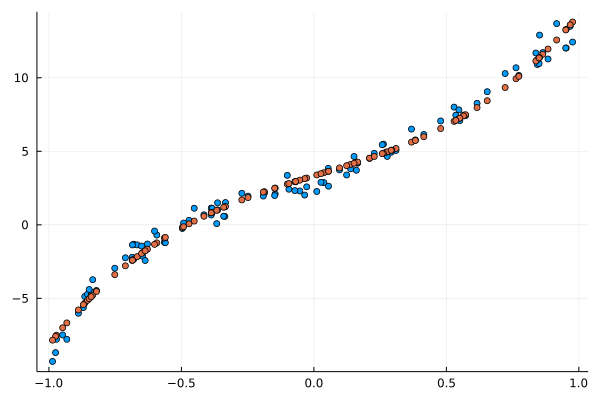
\includegraphics[width=0.7\columnwidth]{graphics/Chap06/Chap06LinearRegressionFit.png}
\caption[]{The blue dots are data while the orange dots are the fit to the data.}
    \label{fig:RegressionDebugging}
\end{figure}

\begin{tcolorbox}[title={\bf \Large Secret to Building Functions is to Check Them While Building Them}]

\textbf{Remarks:}
\begin{itemize}
    \item We broke our goal into two pieces, one solving an exact system of equations and one solving a least squares problem. 
    \item We included error checking as we went along and tested each piece.
    \item By the time we got to the end, the function that was new to us, one that solves a least squares problem, was a trivial extension of something familiar to us, solving a square system of equations with an invertible matrix.
    \item \textcolor{red}{\bf \Large You can do this too, even in HW problems:}
    \begin{itemize}
        \item Even when we say to place your code HERE, that code can include calls to other functions that you place in the same cell.
        \item {\bf \Large Really? Yes. Build a function called \texttt{LeastSquares\_Solve(Phi, Y)} that returns \texttt{alphaStar}}
    \end{itemize}
\end{itemize}
    
\end{tcolorbox}



\begin{lstlisting}[language=Julia,style=mystyle]
# Function for fitting data with Least Squares
function LeastSquares_Solve(Phi, Y)
    ### BEGIN SOLUTION

    ### END SOLUTION
    return alphaStar
end
\end{lstlisting}
\textbf{Output} 
\begin{verbatim}
LeastSquares_Solve (generic function with 1 method)
\end{verbatim}

\begin{lstlisting}[language=Julia,style=mystyle]
# Function for solving Ax=b using LU decomposition
function Exact_Solve(A,b,aTol=1e-10)
    nRows, nCols = size(A)
    if (length(b) !== nRows)||( nRows !== nCols)
         println("System of equations not properly formed")
        return x=NaN
    end
    F=lu(A,check=false)
    display(F)
    #indicesDiagUsmall=findall(x->x<aTol, abs.(diag(F.U)))
    if minimum(abs.(diag(F.U))) < aTol
        println("diagU has numbers that are nearly zero")
        return x=NaN 
    else
        y=forwardsub(F.L,F.P*b)
        x=backwardsub(F.U, y)
        return x 
    end
end


# Function for fitting data with Least Squares
function LeastSquares_Solve(Phi, Y)
    ### BEGIN SOLUTION
    alphaStar = Exact_Solve(Phi'*Phi, Phi'*Y) # Phi'*Y = Phi'*Phi * alpha
    ### END SOLUTION    
   return alphaStar
end
\end{lstlisting}
\textbf{Output} 
\begin{verbatim}
LeastSquares_Solve (generic function with 1 method)
\end{verbatim}

% \begin{lstlisting}[language=Julia,style=mystyle]

% \end{lstlisting}
% \textbf{Output} 
% \begin{verbatim}

% \end{verbatim}

% \begin{lstlisting}[language=Julia,style=mystyle]

% \end{lstlisting}
% \textbf{Output} 
% \begin{verbatim}

% \end{verbatim}

% \begin{lstlisting}[language=Julia,style=mystyle]

% \end{lstlisting}
% \textbf{Output} 
% \begin{verbatim}

% \end{verbatim}


\section{(Optional Read) Fitting a Surface to Data}

\begin{center}
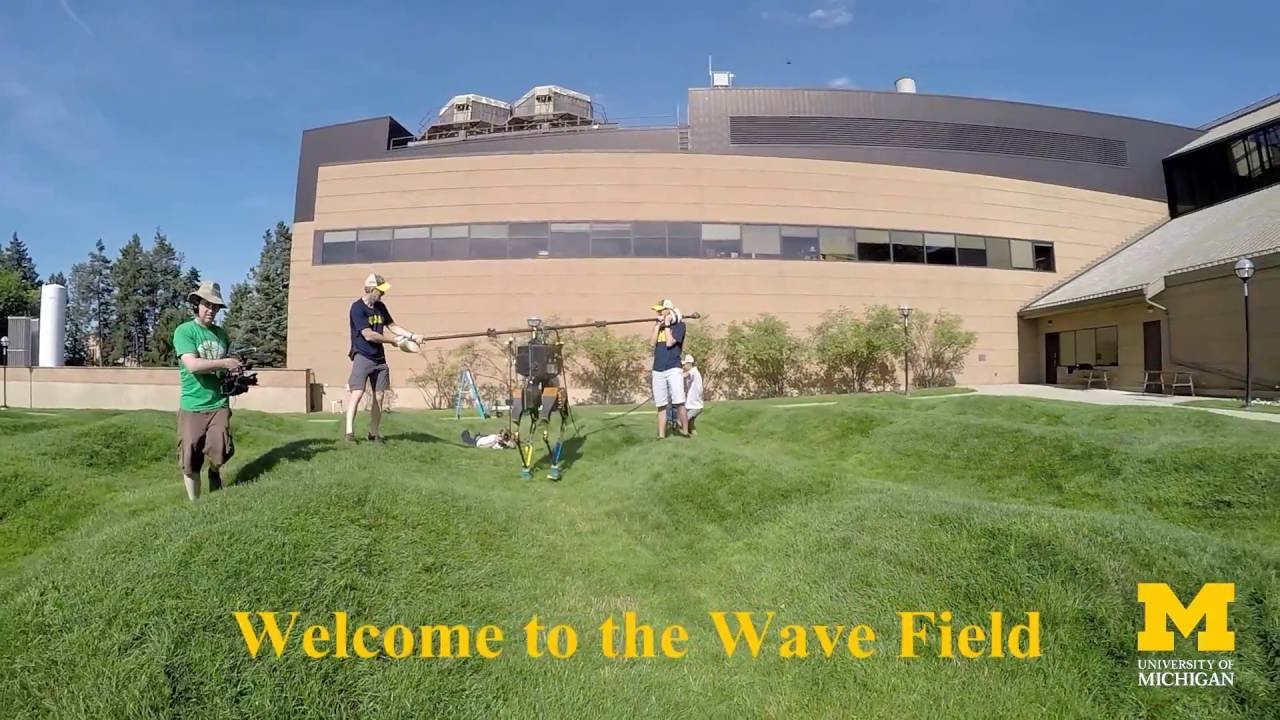
\includegraphics[width=0.8\columnwidth]{graphics/Chap06/WaveFieldMarlo.jpg}
\end{center}

We'll show that fitting a surface to data is the same as fitting a curve to data. Here, we'll continue using monomials as our basis functions. In Project 2, you will use radial basis functions, a better basis for surfaces with lots of curvature.\\


\begin{lstlisting}[language=Julia,style=mystyle]
# run me, don't change me
#
println("Be patient. It takes time to load the Distributions package.")
using Distributions
using Plots
using Pkg
Pkg.add("PyPlot")
\end{lstlisting}
\textbf{Output} 
\begin{verbatim}
Be patient. It takes time to load the Distributions package.

 Info: Precompiling Plots [91a5bcdd-55d7-5caf-9e0b-520d859cae80]
 @ Base loading.jl:1317
\end{verbatim}


\begin{lstlisting}[language=Julia,style=mystyle]
# Attempting to make the Wavefield!
z(x,y) = 0.2*sin(pi*x/2) - 0.2*cos(pi*y/3) + rand(Uniform(-0.03,0.03))

N = 100
Nsq = N^2
X = zeros(Nsq, 1)
Y = zeros(Nsq, 1)
Z = zeros(Nsq, 1)
for i = 1:N
    for j = 1:N
        X[(i-1)*N+j] = 10.0*i/N
        Y[(i-1)*N+j] = 10.0*j/N
        Z[(i-1)*N+j] = z(X[(i-1)*N+j], Y[(i-1)*N+j])
    end
end
scatter(X, Y, Z, marker_z=Z, legend=false, color = :greens, colorbar=true, camera=(-60, 60))
#png("WaveFieldData")
\end{lstlisting}
\textbf{Output} 
\begin{verbatim}
 Info: Precompiling GR_jll [d2c73de3-f751-5644-a686-071e5b155ba9]
 @ Base loading.jl:1317
 Warning: Module Cairo_jll with build ID 23135458039207652 is missing from the cache.
 This may mean Cairo_jll [83423d85-b0ee-5818-9007-b63ccbeb887a] does not support 
precompilation but is imported by a module that does.
 @ Base loading.jl:1008
 Info: Skipping precompilation since __precompile__(false). 
 Importing GR_jll [d2c73de3-f751-5644-a686-071e5b155ba9].
 @ Base loading.jl:1025
 Info: Precompiling Qt5Base_jll [ea2cea3b-5b76-57ae-a6ef-0a8af62496e1]
@ Base loading.jl:1317
 Warning: Module Glib_jll with build ID 23135459152168067 is missing from the cache.
 This may mean Glib_jll [7746bdde-850d-59dc-9ae8-88ece973131d] does not support 
precompilation but is imported by a module that does.
 @ Base loading.jl:1008
Info: Skipping precompilation since __precompile__(false). 
Importing Qt5Base_jll [ea2cea3b-5b76-57ae-a6ef-0a8af62496e1].
 @ Base loading.jl:1025
 Warning: camera: -60° not in [0°, 90°]
 @ Plots /opt/julia/packages/Plots/PomtQ/src/backends/gr.jl:1438
\end{verbatim}

\vspace*{.2cm}

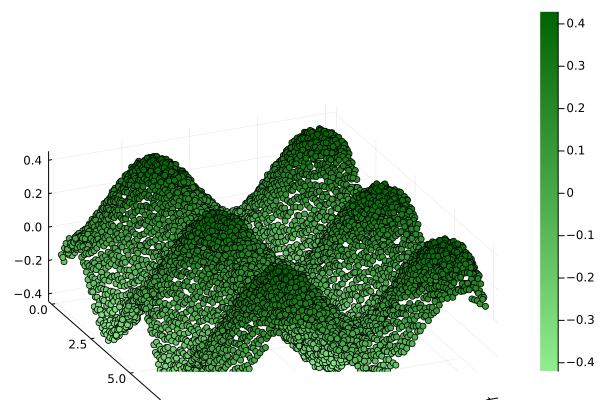
\includegraphics[width=0.7\columnwidth]{graphics/Chap06/WaveFieldData.png}

\vspace*{.2cm}

\begin{lstlisting}[language=Julia,style=mystyle]
using LinearAlgebra

# Function for solving Ax=b using LU decomposition
function solveAxEqb(A,b,aTol=1e-10)
    nRows, nCols = size(A)
    if (length(b) !== nRows)||( nRows !== nCols)
         println("System of equations not properly formed")
        return x=undef
    end
    F=lu(A)
    indicesDiagUsmall=findall(x->x<aTol, abs.(diag(F.U)))
    if length(indicesDiagUsmall) > 0
        println("diagU has numbers that are nearly zero")
        return x=undef
    else
        y=forwardsub(F.L,F.P*b)
        x=backwardsub(F.U, y)
        return x 
    end
end

# Function for fitting data with Least Squares
function LeastSquares_Solve(Phi, Z)
    alpha = solveAxEqb(Phi'*Phi, Phi'*Z) # Phi'*Z = Phi'*Phi * alpha
    Zhat = Phi*alpha
    Error = Z-Zhat
    SqError = Error'*Error
    MeanError = sqrt( SqError/length(Z) )
    return Zhat, Error, SqError, MeanError
end
\end{lstlisting}
\textbf{Output} 
\begin{verbatim}
LeastSquares_Solve (generic function with 1 method)
\end{verbatim}

\begin{lstlisting}[language=Julia,style=mystyle]
# Creating regressor matrix Phi as polynomial fitting
# We include from a constant term, linear terms, quadratic terms, 
# and stop after adding cubic terms
Phi = [ones(Nsq,1) X Y X.^2 Y.^2 X.*Y X.^3 Y.^3 (X).*(Y.^2) (Y).*(X.^2)]
Zhat, Error, SqError, MeanError = LeastSquares_Solve(Phi, Z)
println("Squared error = $SqError and Mean Error = $MeanError")
println("The root mean squared error of our fit is $(MeanError*1e3) mm
    or, if you prefer $(MeanError*1e2/2.54) inches")
\end{lstlisting}
\textbf{Output} 
\begin{verbatim}
Squared error = [260.2866352193259] and Mean Error = [0.16133401229106215]
The root mean squared error of our fit is [161.33401229106215] mm
    or, if you prefer [6.351732767364652] inches
\end{verbatim}


\begin{lstlisting}[language=Julia,style=mystyle]
# Make a scatter plot of Zhat
println("Note how bad the fit is...it does not look like the wavefield at all.")
scatter(X, Y, Zhat, marker_z=Error, legend=false, color = :greens, colorbar=true, camera=(-60, 60))
#png("WaveFieldFit01")
\end{lstlisting}
\textbf{Output} 
\begin{verbatim}
Note how bad the fit is...it does not look like the wavefield at all.
\end{verbatim}

\vspace*{.2cm}

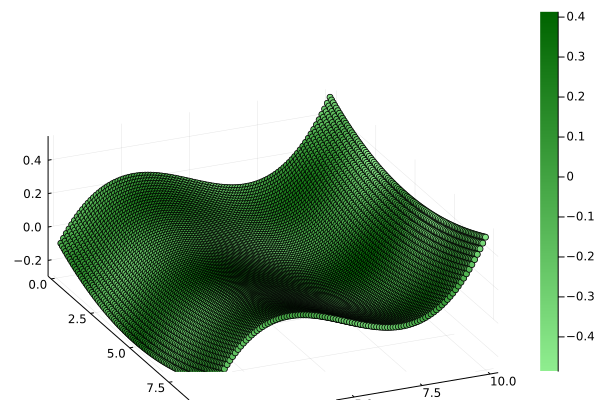
\includegraphics[width=0.7\columnwidth]{graphics/Chap06/WaveFieldFit01.png}


\vspace*{.2cm}

\begin{lstlisting}[language=Julia,style=mystyle]
# Make a scatter plot of the error
println("The fit is so bad, the error looks like the wave field!!!")
scatter(X, Y, Error, marker_z=Error, legend=false, color = :greens, colorbar=true, camera=(-60, 60))
#png("WaveFieldFit01Error")
\end{lstlisting}
\textbf{Output} 
\begin{verbatim}
The fit is so bad, the error looks like the wave field!!!
\end{verbatim}


\vspace*{.2cm}

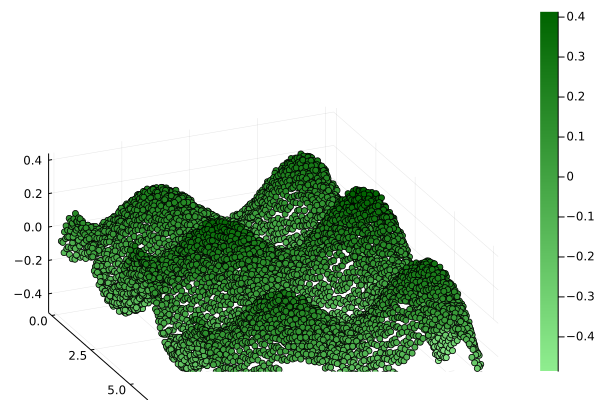
\includegraphics[width=0.7\columnwidth]{graphics/Chap06/WaveFieldFit01Error.png}

\vspace*{.2cm}

\begin{lstlisting}[language=Julia,style=mystyle]
# We'll take another crack at it, using a method that makes it painless to include more terms

# Using for loop to build the regressor matrix Phi
m=8
Phi= Array{Float64,2}(undef, Nsq, 0)
avgX=mean(X)
avgY=mean(Y)
k=0
for i=0:m
    for j=0:m-i
        k=k+1
        Phi=[Phi ((X.-avgX).^i).*((Y.-avgY).^j)/(factorial(i)*factorial(j))]
    end
end
Zhat, Error, SqError, MeanError = LeastSquares_Solve(Phi, Z)
println("Squared error = $SqError and Mean Error = $MeanError")
println("Now see what you think of the fit!")
scatter(X, Y, Zhat, marker_z=Error, legend=false, color = :greens, colorbar=true, camera=(-60, 60))
#png("WaveFieldFit02")
\end{lstlisting}
\textbf{Output} 
\begin{verbatim}
Squared error = [5.066187463106273] and Mean Error = [0.022508192870833218]
Now see what you think of the fit!
\end{verbatim}


\vspace*{.2cm}


\includegraphics[width=0.7\columnwidth]{graphics/Chap06/WaveFieldFit02.png}


\vspace*{.2cm}

\begin{lstlisting}[language=Julia,style=mystyle]
# Make a scatter plot of the error
println("Now, that's what I call a small error plot.")
scatter(X, Y, Error, marker_z=Error, legend=false, color = :greens, colorbar=true, camera=(-60, 60))
#png("WaveFieldFit02Error")
\end{lstlisting}
\textbf{Output} 
\begin{verbatim}
Now, that's what I call a small error plot.
\end{verbatim}
\includegraphics[width=0.7\columnwidth]{graphics/Chap06/WaveFieldFit02Error.png}

\section{(Optional Read) Lab 6.5 A Potpourri of Interesting Commands}

While the tools/commands covered here are not essential for ROB 101, they can make programming either more rewarding or more fun.

\subsection{Using the Benchmark Tool: Which is Faster for Solving Ax=b? }

\begin{lstlisting}[language=Julia,style=mystyle]
using Pkg
Pkg.add("BenchmarkTools")

using LinearAlgebra

function backwardsub(U, b)
    n = length(b)
    x = Vector{Float64}(undef, n) 
    x[n] = b[n]/U[n,n]
    for i in n-1:-1:1
        x[i]=(b[i]- (U[i,(i+1):n])' *x[(i+1):n] )/U[i,i]
    end
    return x
end

function forwardsub(L, b)
    n = length(b)
    x = Vector{Float64}(undef, n) 
    x[1] = b[1]/L[1,1] 
    for i = 2:n 
        x[i]=(b[i]- (L[i,1:i-1])' *x[1:i-1] )/L[i,i] 
    end
    return x
end

function lu_solve(A,b)
    F=lu(A)
    y=forwardsub(F.L,b[F.p])
    x=backwardsub(F.U, y)
    return x
end

function inv_solve(A, b)
    invA = inv(A)
    x = invA*b
    return x
end
\end{lstlisting}
\textbf{Output} 
\begin{verbatim}
inv_solve (generic function with 1 method)
\end{verbatim}

\begin{lstlisting}[language=Julia,style=mystyle]
# We run this cell to compile the functions before using the Benchmark Tool
using Random
Random.seed!(6969420)
N=3
A = rand(N, N)
b = rand(N)
x_inv = inv_solve(A, b)
x_lu = lu_solve(A, b);
\end{lstlisting}
\textbf{Output} 
\begin{verbatim}
Nothing. 
\end{verbatim}

Now, we check the relative speed of the two solvers, using the benchmark tool.
\vspace*{.2cm}
\begin{lstlisting}[language=Julia,style=mystyle]
using BenchmarkTools
Random.seed!(6969420)
N=1000
A = rand(N, N)
b = rand(N)
@benchmark x_inv = inv_solve(A, b)
\end{lstlisting}
\textbf{Output} 

\includegraphics[width=0.7\columnwidth]{graphics/Chap06/BenchmarkInvFunction.png}

\vspace*{.2cm}
\begin{lstlisting}[language=Julia,style=mystyle]
@benchmark x_lu = lu_solve(A, b)
\end{lstlisting}
\textbf{Output} \\

\includegraphics[width=0.7\columnwidth]{graphics/Chap06/BenchmarkLUSolution.png}%

\subsection{Printing with Style and Macros @}


\begin{lstlisting}[language=Julia,style=mystyle]
printstyled("Haha\n", color=:light_cyan)
printstyled("I love ROB 101\n", color=:red, bold=true)
\end{lstlisting}
\textbf{Output} 
\includegraphics[width=0.7\columnwidth]{graphics/Chap06/PrintingWithStyle.png}%


\begin{lstlisting}[language=Julia,style=mystyle]
? printstyled
\end{lstlisting}
\textbf{Output} 
\begin{verbatim}
search: printstyled

printstyled([io], xs...; bold::Bool=false, color::Union{Symbol,Int}=:normal)
Print xs in a color specified as a symbol or integer, optionally in bold.

color may take any of the values :normal, :default, :bold, :black, 
:blink, :blue, :cyan, :green, :hidden, :light_black, 
:light_blue, :light_cyan, :light_green, :light_magenta, 
:light_red, :light_yellow, :magenta, :nothing, :red, :reverse, 
:underline, :white, or :yellow or an integer between 0 and 255 
inclusive. Note that not all terminals support 256 colors. 
If the keyword bold is given as true, the result will be printed in bold.
\end{verbatim}


\begin{lstlisting}[language=Julia,style=mystyle]
macro add_69(num)
    return num+69
end
\end{lstlisting}
\textbf{Output} 
\begin{verbatim}
@add_69 (macro with 1 method)
\end{verbatim}

\begin{lstlisting}[language=Julia,style=mystyle]
@add_69 420
\end{lstlisting}
\textbf{Output} 
\begin{verbatim}
489
\end{verbatim}


\begin{lstlisting}[language=Julia,style=mystyle]
macro add_three_of_them(a, b, c)
    return a+b+c
end
\end{lstlisting}
\textbf{Output} 
\begin{verbatim}
@add_three_of_them (macro with 1 method)
\end{verbatim}

\begin{lstlisting}[language=Julia,style=mystyle]
@add_three_of_them 1 2 3
\end{lstlisting}
\textbf{Output} 
\begin{verbatim}
6
\end{verbatim}

\begin{lstlisting}[language=Julia,style=mystyle]
macro print_in_yellow(x)
    printstyled(x, color=:yellow)
end
\end{lstlisting}
\textbf{Output} 
\begin{verbatim}
@print_in_yellow (macro with 1 method)
\end{verbatim}

\begin{lstlisting}[language=Julia,style=mystyle]
@print_in_yellow "My name is... My name is... My name is... SLIM SHADY"
\end{lstlisting}
\textbf{Output} 

\includegraphics[width=0.7\columnwidth]{graphics/Chap06/PrintInYellow.png}%

\textbf{Julia has an amazing list of Emojis that you can copy and paste into your cells. The symbols will not print in the latex code box below, but they will print in Julia: \url {https://emojidb.org/julia-and-julia-emojis}}

\begin{lstlisting}[language=Julia,style=mystyle]
macro aggressive_print(x)
    s = uppercase(x)
    s*= "!!!!     " # s*= appends the string between the quote marks
                    # The characters do not show here but do work in Julia; see below.
    printstyled(s, color=:red)
end
\end{lstlisting}
\textbf{Output} 
\begin{verbatim}
@aggressive_print (macro with 1 method)
\end{verbatim}


\begin{lstlisting}[language=Julia,style=mystyle]
@aggressive_print "hi nice to meet you"
\end{lstlisting}
\textbf{Output} 



\includegraphics[width=1.0\columnwidth]{graphics/Chap06/AggressivePrint.png}%

\subsection{Multiple Dispatch and Function Overloading}


\begin{lstlisting}[language=Julia,style=mystyle]
function add_them(a::Int, b::Int)
    result = a+b
    return result
end

function add_them(a::Int, b::Vector)
    result = a .+ b
    return result
end

function add_them(a::String, b::Int)
    result = a*string(b)
    return result
end

function add_them(a::String, b::Vector) 
    result = a
    for s in b result*=string(s) end
    return result
end
\end{lstlisting}
\textbf{Output} 
\begin{verbatim}
add_them (generic function with 4 methods)
\end{verbatim}

\begin{lstlisting}[language=Julia,style=mystyle]
@show add_them(2, 3);
@show add_them(2, [3, 4, 5]);
@show add_them("mrbeast", 6000);
@show add_them("gluckgluck", [9,0,0,0]);
\end{lstlisting}
\textbf{Output} 
\begin{verbatim}
add_them(2, 3) = 5
add_them(2, [3, 4, 5]) = [5, 6, 7]
add_them("mrbeast", 6000) = "mrbeast6000"
add_them("gluckgluck", [9, 0, 0, 0]) = "gluckgluck9000"
\end{verbatim}



\begin{lstlisting}[language=Julia,style=mystyle]
import Base:+ 

function +(a::Int, b::Vector)
    result = a .+ b
    return result
end

function +(a::String, b::Int)
    result = a*string(b)
    return result
end

function +(a::String, b::Vector) 
    result = a
    for s in b result*=string(s) end
    return result
end
\end{lstlisting}
\textbf{Output} 
\begin{verbatim}
+ (generic function with 193 methods)
\end{verbatim}

\begin{lstlisting}[language=Julia,style=mystyle]
@show 2 + [3, 4, 5];
@show "mrbeast" + 6000;
@show "gluckgluck" + [9,0,0,0];
\end{lstlisting}
\textbf{Output} 
\begin{verbatim}
2 + [3, 4, 5] = [5, 6, 7]
"mrbeast" + 6000 = "mrbeast6000"
"gluckgluck" + [9, 0, 0, 0] = "gluckgluck9000"
\end{verbatim}


\chapter{Julia Lab 7: Grahm-Schmidt Algorithm, Orthogonal (Basis) Vectors, and Computing the Null Space}
\label{chap:Lab7}
\section*{Learning Objectives}

\begin{itemize}
\item Master the Gram-Schmidt algorithm
\item Explore some of its uses
\item Regression
\item Debugging, or finding and fixing errors in your code
\end{itemize}

\section*{Outcomes} 
\begin{itemize}
\item In a set of orthogonal vectors, each vector forms a right angle with respect to the other vectors in the set
\item If a vector is non-zero, we can easily normalize its length to one
\item In a set of orthonormal vectors, each vector has length one and forms a right angle with respect to the other vectors in the set 
\item Gram-Schmidt applied to a set of linearly independent vectors produces a set of orthogonal vectors, and with one small modification, we can produce a set of orthonormal vectors
\item Gram-Schmidt provides an easy way to compute the null space of a matrix
\end{itemize}

\vspace*{1cm}

\textbf{Either download Lab7 from our Canvas site or open up a Jupyter notebook so that you can enter code as we go. It is suggested that you have line numbering toggled on.}  

\newpage

This lab goes all in on the Gram-Schmidt Process. When you are done with the lab, you should feel that you ``own'' the algorithm. \\

Julia has a command for computing the inner product, aka dot product, of two vectors. Surprise, the command is called \texttt{dot}. We'll show you how to use it.

\begin{lstlisting}[language=Julia,style=mystyle]
# The dot comamnd is part of the LinearAlgebra package.
#
using LinearAlgebra
#
u = [1, 2, 3, 4, 5]
v = [6, 7, 8, 9, 10]

uDOTv = dot(u,v)
\end{lstlisting}
\textbf{Output} 
\begin{verbatim}
130
\end{verbatim}
You can easily compute the dot product without the LinearAlgebra Package. 

\begin{lstlisting}[language=Julia,style=mystyle]
# The dot command computes u'*v; here is the proof!
u'*v 
\end{lstlisting}
\textbf{Output} 
\begin{verbatim}
130
\end{verbatim}

Normalizing the length of vectors to one is a pain by hand. But in Julia, it's such a snap that we will soon incorporate it directly into the Gram-Schmidt process. 

\begin{lstlisting}[language=Julia,style=mystyle]
# The norm command is part of the LinearAlgebra Package, which we already ran
@show norm(v)
w = v /norm(v)
@show norm(w)
w 
\end{lstlisting}
\textbf{Output} 
\begin{verbatim}
norm(v) = 18.16590212458495
norm(w) = 1.0

5-element Vector{Float64}:
 0.3302891295379082
 0.3853373177942262
 0.4403855060505443
 0.4954336943068623
 0.5504818825631803
\end{verbatim}

\section{Orthogonal Vectors}

Suppose that $\{ u_1, u_2\}$ is a set of linearly independent vectors. The Gram-Schmidt Process builds from them an orthogonal set of vectors that spans the same set of vectors as $\{ u_1, u_2\}$. It works as follows:\\

\textbf{Step 1:} $v_1 := u_1$ \\

\textbf{Step 2:} $v_2 := u_2  - a_2 v_1$, where we seek to choose $a_2$ such that $v_2 \bullet v_1 = 0$. We compute
\begin{align*}
    v_2 \bullet v_1 &  = \left( u_2  - a_2 v_1 \right) \bullet  v_1 \\
    &= u_2 \bullet v_1 - a_2 v_1 \bullet v_1.
\end{align*}
If $ v_1 \bullet v_1\neq 0$, then we can set $u_2 \bullet v_1 - a_2 v_1 \bullet v_1 = 0$ and solve for $a_2$, namely
$$a_2 = \frac{u_2 \bullet v_1}{v_1 \bullet v_1}. $$
\\

\begin{tcolorbox}
\textbf{Important Formula to Build $\boldsymbol{v_1 \perp v_2}$ from $\boldsymbol{u_1}$ and $\boldsymbol{u_2}$ while Preserving Spans}
\begin{equation}
    \label{eq:OrthognalProjection01}
    \begin{aligned}
    v_1 &= u_1\\
    v_2 &= u_2 -  \left(\frac{u_2 \bullet v_1}{v_1 \bullet v_1}\right) v_1\\
    \\ 
    \spanof{v_1}&=\spanof{u_1}\\
    \spanof{v_1, v_2}&= \spanof{u_1, u_2}
     \end{aligned}
\end{equation}
\end{tcolorbox}

We illustrate the above step by step.

\begin{lstlisting}[language=Julia,style=mystyle]
using Random
Random.seed!(2022)
u1 = rand(4,1)
u2 = rand(4,1)
U = [u1 u2]
@show det(U'*U) # non-zero means u1 and u2 are independent
# G-S on two vectors (see grey box above)
@show v1 = u1
@show v2 = u2 - ( dot(u2,v1)/dot(v1,v1) )*v1
V = [v1 v2]
@show dot(v1,v2) # should be zero
println(" ") # Will print a space
@show det(V'*V) # non-zero means v1 and v2 are independent
V
\end{lstlisting}
\textbf{Output} 
\begin{verbatim}
det(U' * U) = 0.32941782975491707
v1 = u1 = [0.7982589547203172; 0.8998485508054206; 0.15010598805721265;
0.1749482291443072]
v2 = u2 - (dot(u2, v1) / dot(v1, v1)) * v1 = [-0.04289157616244632; -0.07773177980842272;
0.3598021757771466; 0.28681029417179305]
dot(v1, v2) = -1.2642012348321895e-17
 
det(V' * V) = 0.32941782975491707

4×2 Matrix{Float64}:
 0.798259  -0.0428916
 0.899849  -0.0777318
 0.150106   0.359802
 0.174948   0.28681
\end{verbatim}

\begin{lstlisting}[language=Julia,style=mystyle]
v1=v1/norm(v1)  
v2=v2/norm(v2)
# 
V= [v1 v2]  # now columns are orthonormal vectors
@show det(V'*V) # non-zero implies linearly independent
@show V'*V - [v1'*v1  v1'*v2; v2'*v1 v2'*v2]
V'*V
\end{lstlisting}
\textbf{Output} 
\begin{verbatim}
det(V' * V) = 1.0000000000000004
V' * V - [v1' * v1  v1' * v2; v2' * v1  v2' * v2] = [0.0 0.0; 0.0 0.0]

2×2 Matrix{Float64}:
  1.0          -1.34268e-17
 -1.34268e-17   1.0
\end{verbatim}


\begin{lstlisting}[language=Julia,style=mystyle]
# A helper function to zero out small entries of a matrix or vector
function cleanUp(A,tol=1e-10)
    B=copy(A)
    indicesSmall=findall(x->x<tol, abs.(B))
    B[indicesSmall]=0.0*abs.(B[indicesSmall])
    return B
end
\end{lstlisting}
\textbf{Output} 
\begin{verbatim}
cleanUp (generic function with 2 methods)
\end{verbatim}


\begin{lstlisting}[language=Julia,style=mystyle]
cleanUp(V'*V)
\end{lstlisting}
\textbf{Output} 
\begin{verbatim}
2×2 Matrix{Float64}:
 1.0  0.0
 0.0  1.0
\end{verbatim}

\section{The Span Condition}

Next will check that $\spanof{u_1, u_2} = \spanof{v_1, v_2}$, where we recall that computing the span of a set of vectors means determining ``all possible linear combinations'', which seems like a lot of work! However, if we show that
\begin{align}
\label{eq:u1}
    u_1 & \in \spanof{v_1, v_2}\\
\label{eq:u2}
    u_2 & \in \spanof{v_1, v_2},
\end{align}
it then follows that $\spanof{u_1, u_2} \subset \spanof{v_1, v_2}$. If we also show that
\begin{align}
\label{eq:v1}
    v_1 & \in \spanof{u_1, u_2} \\
\label{eq:v2}
    v_2 & \in \spanof{u_1, u_2}, 
\end{align}
we'll have that $\spanof{v_1, v_2} \subset \spanof{u_1, u_2}$. Moreover, for any two \textbf{subsets} $A$ and $B$, the conditions $A \subset B$ and $B \subset A$ are equivalent to $A=B$. Applying this to $\spanof{u_1, u_2}$ and $\spanof{v_1, v_2}$, yields
$$\big(\spanof{u_1, u_2} \subset \spanof{v_1, v_2}\big) \text{\bf and } \big(\spanof{v_1, v_2} \subset \spanof{u_1, u_2} \big) \iff \big(\spanof{u_1, u_2} = \spanof{v_1, v_2}\big).$$

Because $u_1 = v_1$, the conditions \eqref{eq:u1} and \eqref{eq:v1} are immediate. Hence, we only need to show conditions \eqref{eq:u2} and \eqref{eq:v2}, 
% \begin{align*}
%     u_2 & \in \spanof{v_1, v_2}\\
%     & \text{and} \\
%     v_2 & \in \spanof{u_1, u_2}, \\
% \end{align*}
that is, $u_2$ can be written as a linear combination of $v_1$ and $v_2$, and similarly, $v_2$ can be written as a linear combination of $u_1$ and $u_2$.\\

In our textbook, we show these conditions analytically. Below, we verify them in code!\\

\begin{lstlisting}[language=Julia,style=mystyle]
# We check the span conditions
# including the obvious: u1 = v1 and v1 = u1
@show u1 - v1 
println(" ")
# define
a1 = -dot(u2,v1)/dot(v1,v1)
a2 = 1
# check v2 =  a*u1 + a2*u2 
@show v2 - (a1*u1 + a2*u2)
println(" ")
# define
b1 = dot(u2,v1)/dot(v1,v1)
b2 = 1
# check u2 =  b1*v1 + b2*v2 
@show u2 - (b1*v1 + b2*v2)
\end{lstlisting}
\textbf{Output} 
\begin{verbatim}
u1 - v1 = [0.0; 0.0; 0.0; 0.0]
 
v2 - (a1 * u1 + a2 * u2) = [0.0; 0.0; 0.0; 0.0]
 
u2 - (b1 * v1 + b2 * v2) = [0.0; 0.0; 0.0; 0.0]

4×1 Matrix{Float64}:
 0.0
 0.0
 0.0
 0.0
\end{verbatim}

Here are the analytical calculations, in case you are interested,
$$ \large
 \begin{aligned}
 v_1 & = u_1 \\
 v_2 &= u_2 - \left(\frac{u_2 \bullet v_1}{v_1 \bullet v_1}\right) v_1 \\
	\end{aligned}
$$
we deduce that
$$\boxed{\bf  \large  v_2 = a_1 u_1 + a_2 u_2 } $$
with 
$$  \large
 \begin{aligned}
a_1 &= -\left(\frac{u_2 \bullet v_1}{v_1 \bullet v_1}\right)\\
a_2 &= 1
\end{aligned}
$$
and
 $$ \boxed{ \bf \large u_2 = b_1 v_1 + b_2 v_2}$$
with 
$$  \large
 \begin{aligned}
b_1 &=  \left(\frac{u_2 \bullet v_1}{v_1 \bullet v_1}\right)\\
b_2 &= 1
\end{aligned}
$$

\section{Graphical Interpretation of Orthogonal Vectors and Another way to Understand the Span Condition}

Figure~\ref{fig:OrthognalVectors} provides a graphical illustration of the action of Gram-Schmidt on a pair of linearly independent vectors $\{u_1, u_2 \}$. Figure~\ref{fig:OrthognalVectors}-(a) shows two randomly generated vectors. Then we apply \textbf{Gram-Schmidt with normalization to produce orthonormal vectors} $\{v_1, v_2 \}$, as shown in Fig.~\ref{fig:OrthognalVectors}-(b).
$$
    \begin{aligned}
    v_1 &= u_1\\
    v_1 &= v_1/||v_1|| \\
    v_2 &= u_2 -  \left(u_2 \bullet v_1 \right) v_1\\
    v_2 & = v_2/||v_2||
     \end{aligned}
$$


\begin{figure}[hbt!]%
\centering
\subfloat[]{%
    \label{fig:u1u2}%
	\centering
\includegraphics[width=0.45\columnwidth]{graphics/Chap07/u1u2.png}}%
\hspace{5pt}%
\subfloat[]{%
    \label{fig:v1v2}%
	\centering
\includegraphics[width=0.45\columnwidth]{graphics/Chap07/v1v2.png}}%
\hspace{5pt}%
\subfloat[]{%
    \label{fig:u2v1v2}%
	\centering
\includegraphics[width=0.45\columnwidth]{graphics/Chap07/u2v1v2.png}}%
\hspace{5pt}%
    \subfloat[]{%
    \label{fig:u2v1plusv2}%
	\centering
\includegraphics[width=0.45\columnwidth]{graphics/Chap07/u2v1plusv2.png}}%
    \caption[]{What does Gram-Schmidt do to a pair of linearly independent vectors? (a) $\{u_1, u_2 \}$ are linearly independent, but they do not form a right angle. (b) $\{v_1, v_2 \}$ is an \textbf{orthonormal} set produced by applying Gram-Schmidt to $\{u_1, u_2 \}$. They clearly form a right angle. (c)  The thin blue vector is $(u_2 \bullet v_1)\cdot v_1$. It goes by two names, the projection of $u_2$ along the direction $v_1$ or the component of $u_2$ along the direction $v_1$. The thin green vector is $(u_2 \bullet v_2)\cdot v_2$. It goes by two names, the projection of $u_2$ along the direction $v_2$ or the component of $u_2$ along the direction $v_2$. (d) From Gram-Schmidt, we know that $u_2 = (u_2 \bullet v_1)\cdot v_1 +(u_2 \bullet v_2)\cdot v_2 $. This last plot shows the addition of the two vectors using the head to tail notion of vector addition that you may have come across in a physics course.}
    \label{fig:OrthognalVectors}
\end{figure}

 Because $\spanof{v_1, v_2}= \spanof{u_1, u_2}$, we know that we can express $u_1$ and $u_2$ as linear combinations of $v_1$ and $v_2$. When $\{v_1, v_2 \}$ are \textbf{orthonormal}, it is very easy to compute the linear combinations
$$
\begin{aligned}
u_1 & =   \underbrace{\left(u_1 \bullet v_1 \right)}_{\alpha_1} v_1 +  \underbrace{\left(u_1 \bullet v_2 \right)}_{\alpha_2} v_2 = \alpha_1 v_1 + \alpha_2 v_2\\
\\
u_2 & =   \underbrace{\left(u_2 \bullet v_1 \right)}_{\beta_1} v_1 +  \underbrace{\left(u_2 \bullet v_2 \right)}_{\beta_2} v_2 = \beta_1 v_1 + \beta_2 v_2.
\end{aligned}
$$
Yes, it is worth repeating: when $\{v_1, v_2 \}$ are \textbf{orthonormal}, computing the coefficients in the linear combination is very easy. Figure~\ref{fig:OrthognalVectors}-(c) shows the vector $u_2$ and the two parts of its linear combination in terms of $\{v_1, v_2 \}$; namely, the thin blue vector is the component of $u_2$ along $v_1$, namely $\left(u_2 \bullet v_1 \right) v_1$, while the thin green line is the component of $u_2$ along $v_2$, namely $\left(u_2 \bullet v_2 \right) v_2$. Figure~\ref{fig:OrthognalVectors}-(d) shows that indeed, $u_2 =   \left(u_2 \bullet v_1 \right) v_1 +  \left(u_2 \bullet v_2 \right) v_2$, the sum of the two components.\\

When $\{v_1, v_2 \}$ are \textbf{orthogonal but not orthonormal}, the expressions are still quite handy,
$$
\begin{aligned}
u_1 & =   \underbrace{\left(\frac{u_1 \bullet v_1}{v_1 \bullet v_1}\right)}_{\alpha_1} v_1 +  \underbrace{\left(\frac{u_1 \bullet v_2}{v_2 \bullet v_2}\right)}_{\alpha_2} v_2 = \alpha_1 v_1 + \alpha_2 v_2\\
\\
u_2 & =   \underbrace{\left(\frac{u_2 \bullet v_1}{v_1 \bullet v_1}\right)}_{\beta_1} v_1 +  \underbrace{\left(\frac{u_2 \bullet v_2}{v_2 \bullet v_2}\right)}_{\beta_2} v_2 = \beta_1 v_1 + \beta_2 v_2.
\end{aligned}
$$

\begin{lstlisting}[language=Julia,style=mystyle]
# This code generates the plots in Figure 7.1
using Random
Random.seed!(31415926535897932384626433)
u1 = 3*randn(2,1)
u2 = 4*randn(2,1)
u1=[3; 2]
u2=[2; 4]
U = [u1 u2]
@show det(U'*U) # non-zero means independent
# G-S on two vectors (see big green box below)
@show v1 = u1
@show v2 = u2 - ( dot(u2,v1)/dot(v1,v1) )*v1

v1 = v1/norm(v1)
v2 = v2/norm(v2)

t=LinRange(-4, 4,10); t=collect(t)
zero=0.0*t;

p1=plot(t,0.0.*t, color=:black, lw=3, legend=false, aspect_ratio=:equal,framestyle = :origin)
plot!(0.0.*t,t, color=:black, lw=3, legend=false)

plot!([0;u1[1:1]],[0;u1[2:2]], arrow=true, color=:gold, lw=2 )
plot!([0;u2[1:1]],[0;u2[2:2]], arrow=true, color=:black, lw=2 )

p2=plot(t,0.0.*t, color=:black, lw=3, legend=false, aspect_ratio=:equal,framestyle = :origin)
plot!(0.0.*t,t, color=:black, lw=3, legend=false)

plot!([0;v1[1:1]],[0;v1[2:2]], arrow=true, color=:blue, lw=4 )
plot!([0;v2[1:1]],[0;v2[2:2]], arrow=true, color=:green, lw=4 )


p3=plot(t,0.0.*t, color=:black, lw=3, legend=false, aspect_ratio=:equal,framestyle = :origin)
plot!(0.0.*t,t, color=:black, lw=3, legend=false)

u2Projv1 = ( dot(u2,v1)/dot(v1,v1) )*v1
u2Projv2 = ( dot(u2,v2)/dot(v2,v2) )*v2

plot!([0;u2Projv1[1:1]],[0;u2Projv1[2:2]], arrow=true, color=:blue, lw=2 )
plot!([0;u2Projv2[1:1]],[0;u2Projv2[2:2]], arrow=true, color=:green, lw=2 )

plot!([0;v1[1:1]],[0;v1[2:2]], arrow=true, color=:blue, lw=4 )
plot!([0;v2[1:1]],[0;v2[2:2]], arrow=true, color=:green, lw=4 )
plot!([0;u2[1:1]],[0;u2[2:2]], arrow=true, color=:black, lw=2 )


p4=plot(t,0.0.*t, color=:black, lw=3, legend=false, aspect_ratio=:equal,framestyle = :origin)
plot!(0.0.*t,t, color=:black, lw=3, legend=false)

plot!([0;u2[1:1]],[0;u2[2:2]], arrow=true, color=:black, lw=2 )

plot!([0;u2Projv1[1:1]],[0;u2Projv1[2:2]], arrow=true, color=:blue, lw=2 )
plot!([0;u2Projv2[1:1]].+u2Projv1[1:1],[0;u2Projv2[2:2]].+u2Projv1[2:2], arrow=true, color=:green, lw=2 )

display(p1)
display(p2)
display(p3)
display(p4)
\end{lstlisting}
\textbf{Output} 

Plots as shown in Fig.~\ref{fig:OrthognalVectors}, though without the beautiful handwritten labels.


% \begin{lstlisting}[language=Julia,style=mystyle]

% \end{lstlisting}
% \textbf{Output} 
% \begin{verbatim}

% \end{verbatim}

% \begin{lstlisting}[language=Julia,style=mystyle]

% \end{lstlisting}
% \textbf{Output} 
% \begin{verbatim}

% \end{verbatim}

\section{Gram-Schmidt Algorithm on a Set of four Vectors}

The Gram-Schmidt Algorithm takes a set of linearly independent vectors and creates a set of orthogonal vectors that is (i) also linearly independent, and (ii), spans the same subspace as the original vectors. Here is the algorithm written out for a set of four linearly independent vectors. The hope is that you see the pattern and hence are ready to put the algorithm into a \texttt{for\, loop}.\\

\begin{tcolorbox}[sharp corners, colback=green!30, colframe=green!80!blue, title=\textbf{\Large Gram-Schmidt Process for 4 Vectors
}]
Suppose that that the set of vectors $\{ u_1, u_2, u_3, u_4\}$ is linearly independent. Then the vectors  $\{ v_1, v_2, v_3, v_4\}$ are orthogonal, where
$$
 \begin{aligned}
 v_1 & = u_1 \\
 v_2 &= u_2 - \left(\frac{u_2 \bullet v_1}{v_1 \bullet v_1}\right) v_1 \bigskip \\
 v_3 &= u_3 -\left(\frac{u_3 \bullet v_1}{v_1 \bullet v_1}\right) v_1 - \left(\frac{u_3 \bullet v_2}{v_2 \bullet v_2}\right) v_2 \\
 v_4 & = u_4  - \left(\frac{u_4 \bullet v_1}{v_1 \bullet v_1}\right) v_1 - \left(\frac{u_4 \bullet v_2}{v_2 \bullet v_2}\right) v_2 - \left(\frac{u_4 \bullet v_3}{v_3 \bullet v_3}\right) v_3
	\end{aligned}
$$


Could you write out the line for a fifth vector? 
\end{tcolorbox}

\begin{lstlisting}[language=Julia,style=mystyle]
using Random
Random.seed!(2525)
u1 = rand(4,1)
u2 = rand(4,1)
u3 = rand(4,1)
u4 = rand(4,1)
# G-S on four vectors (see big green box)
v1 = u1 # k=1
v2 = u2 - ( dot(u2,v1)/dot(v1,v1) )*v1  # k=2, i = 1:1
v3 = u3 - ( dot(u3,v1)/dot(v1,v1) )*v1 - ( dot(u3,v2)/dot(v2,v2) )*v2 # k=3, i = 1:2
v4 = u4 - ( dot(u4,v1)/dot(v1,v1) )*v1 - ( dot(u4,v2)/dot(v2,v2) )*v2 - ( dot(u4,v3)/dot(v3,v3) )*v3 # k=4, i = 1:3
\end{lstlisting}
\textbf{Output} 
\begin{verbatim}
4×4 Matrix{Float64}:
 2.54741  0.0       0.0        0.0
 0.0      0.183229  0.0        0.0
 0.0      0.0       0.0246929  0.0
 0.0      0.0       0.0        0.643923
\end{verbatim}


We define $V:=\left[ \begin{array}{cccc} v_1 & v_2 & v_3 & v_4 \end{array} \right] $ and note that 
 $$V^\top V = \left[ \begin{array}{c} v_1^\top  \\ v_2^\top \\ v_3^\top \\ v_4 \end{array} \right] \cdot \left[ \begin{array}{cccc} v_1 & v_2 & v_3 & v_4 \end{array} \right] = \left[ \begin{array}{cccc}  
 v_1^\top \cdot v_1 &  v_1^\top \cdot v_2 &  v_1^\top \cdot v_3 &  v_1^\top \cdot v_4  \\
  v_2^\top \cdot v_1 &  v_2^\top \cdot v_2 &  v_2^\top \cdot v_3 &  v_2^\top \cdot v_4  \\
   v_3^\top \cdot v_1 &  v_3^\top \cdot v_2 &  v_3^\top \cdot v_3 &  v_3^\top \cdot v_4  \\
   v_4^\top \cdot v_1 &  v_4^\top \cdot v_2 &  v_4^\top \cdot v_3 &  v_4^\top \cdot v_4
 \end{array} 
  \right],$$
  that is, 
  $$\left[V^\top V \right]_{ij} := v_i^\top \cdot v_j = v_i \bullet v_j .$$
Therefore, if the set $\{ v_1, v_2, v_3, v_4\}$ is orthogonal, we should have
 $$V^\top V = \left[ \begin{array}{c} v_1^\top  \\ v_2^\top \\ v_3^\top \\ v_4 \end{array} \right] \cdot \left[ \begin{array}{cccc} v_1 & v_2 & v_3 & v_4 \end{array} \right] = \left[ \begin{array}{cccc}  
||v_1||^2 & 0 & 0 & 0 \\
0 & ||v_2||^2 & 0 & 0 \\
0 & 0 & ||v_3||^2 & 0\\
0 & 0 & 0 & ||v_4||^2
 \end{array} 
  \right],$$
  where $||v_i||^2 = v_i^\top \cdot v_i.$
We check this.\\
  
\begin{lstlisting}[language=Julia,style=mystyle]
V = [v1 v2 v3 v4]
cleanUp(V'*V)
\end{lstlisting}
\textbf{Output} 
\begin{verbatim}
4×4 Matrix{Float64}:
 2.54741  0.0       0.0        0.0
 0.0      0.183229  0.0        0.0
 0.0      0.0       0.0246929  0.0
 0.0      0.0       0.0        0.643923
\end{verbatim}

After normalization, we obtain ones on the diagonal.
\begin{lstlisting}[language=Julia,style=mystyle]
# Normalize
V = [v1/norm(v1) v2/norm(v2) v3/norm(v3) v4/norm(v4)] 
cleanUp(V'*V)
\end{lstlisting}
\textbf{Output} 
\begin{verbatim}
4×4 Matrix{Float64}:
 1.0  0.0  0.0  0.0
 0.0  1.0  0.0  0.0
 0.0  0.0  1.0  0.0
 0.0  0.0  0.0  1.0
\end{verbatim}

Here is the algorithm written closer to how it looks in a for loop.

\begin{lstlisting}[language=Julia,style=mystyle]
# same algorithm, but written closer to how it looks in a for loop
# 
using Random
Random.seed!(2525)
u1 = rand(4,1)
u2 = rand(4,1)
u3 = rand(4,1)
u4 = rand(4,1)
# G-S on four vectors (see big green box)
v1 = u1 # k=1
#
v2 = u2 # k=2
v2 = v2 - ( dot(u2,v1)/dot(v1,v1) )*v1 # i=1:
#
v3 = u3 # k=3 
v3 = v3 - ( dot(u3,v1)/dot(v1,v1) )*v1 # i=1
v3 = v3 - ( dot(u3,v2)/dot(v2,v2) )*v2 # i=2
#
v4 = u4 # k=4
v4 = v4 - ( dot(u4,v1)/dot(v1,v1) )*v1 # i=1
v4 = v4 - ( dot(u4,v2)/dot(v2,v2) )*v2 # i=2
v4 = v4 - ( dot(u4,v3)/dot(v3,v3) )*v3 # i=3
# Normalize
V = [v1/norm(v1) v2/norm(v2) v3/norm(v3) v4/norm(v4)] 
cleanUp(V'*V)
\end{lstlisting}
\textbf{Output} 
\begin{verbatim}
4×4 Matrix{Float64}:
 1.0  0.0  0.0  0.0
 0.0  1.0  0.0  0.0
 0.0  0.0  1.0  0.0
 0.0  0.0  0.0  1.0
\end{verbatim}

\section{Gram-Schmidt Algorithm for a General Number of Linearly Independent Vectors}

% \begin{tcolorbox}[sharp corners, colback=green!30, colframe=green!80!blue, title=\textbf{\Large Gram-Schmidt Process}]
% Suppose that that the set of vectors $\{ u_1, u_2, \ldots, u_m\}$ is linearly independent and you generate a new set of vectors by 
%  \begin{equation}
%  \label{eq:GramSchmidt}
%  \begin{aligned}
%  v_1 & = u_1 \\
%  v_2 &= u_2 - \left(\frac{u_2 \bullet v_1}{v_1 \bullet v_1}\right) v_1 \bigskip \\
%  v_3 &= u_3 -\left(\frac{u_3 \bullet v_1}{v_1 \bullet v_1}\right) v_1 - \left(\frac{u_3 \bullet v_2}{v_2 \bullet v_2}\right) v_2 \\
%  & ~\vdots \\
% 	v_k &= u_k  - \sum_{i=1}^{k-1} \left(\frac{u_k \bullet v_i}{v_i \bullet v_i}\right) v_i~~~~~\text{(General Step)}
% 	\end{aligned}
% \end{equation}
% Then the set of vectors $\{ v_1, v_2,  \ldots, v_m\}$ is 
% \begin{itemize}
%     \item orthogonal, meaning, $i \neq j \implies v_i \bullet v_j = 0$
%     \item span preserving, meaning that, for all $1 \le k \le m$, 
%     \begin{equation}
%         \label{eq:SpanPreserving}
%         \spanof{v_1, v_2, \ldots, v_k} = \spanof{u_1, u_2, \ldots, u_k},
%     \end{equation} 
%     and
%         \item linearly independent.
% \end{itemize}
% \end{tcolorbox}


The Gram-Schmidt process on a set of linearly independent vectors $\{ u_1, u_2, \ldots, u_m\}$ is as follows 
 \begin{equation}
 \label{eq:GramSchmidt}
 \begin{aligned}
 v_1 & = u_1 \\
 v_2 &= u_2 - \left(\frac{u_2 \bullet v_1}{v_1 \bullet v_1}\right) v_1 \bigskip \\
 v_3 &= u_3 -\left(\frac{u_3 \bullet v_1}{v_1 \bullet v_1}\right) v_1 - \left(\frac{u_3 \bullet v_2}{v_2 \bullet v_2}\right) v_2 \\
 & ~\vdots \\
	v_k &= u_k  - \sum_{i=1}^{k-1} \left(\frac{u_k \bullet v_i}{v_i \bullet v_i}\right) v_i~~~~~\text{(General Step)}
	\end{aligned}
\end{equation}

\begin{tcolorbox}[ title=\textbf{\Large Gram-Schmidt Process as Pseudocode}]

We assume the columns of $U:=\left[ \begin{array}{cccc} u_1 & u_2 & \cdots  & u_m \end{array} \right] $
are linearly independent. We build a set of orthonormal vectors as follows\\
{\rm 
V=[ ] \# blank array\\
\textbf{for} k = 1 : Number of columns of U\\
\hspace*{1cm} uk = U[:,k]\\
\hspace*{1cm} vk =copy(uk)\\
\hspace*{1cm} \textbf{for} i = 1:k-1\\
\hspace*{2cm} vi = V[:,i]\\
\hspace*{2cm} $\mathlarger{vk = vk - \frac{  uk \bullet vi}{vi \bullet vi}  \cdot vi}$\\
\hspace*{1cm} \textbf{end}\\
\hspace*{1cm} V = [V vk/norm(vk)] \\
\textbf{end}
}
\end{tcolorbox}

\begin{lstlisting}[language=Julia,style=mystyle]
# GS in code
# 
using LinearAlgebra
function grahm_schmidt(U)
    nRowsU = size(U,1) # the 1 returns the number of rows
    nColsU = size(U,2) # the 2 returns number of columns. 
    #
    # We first create an empty matrix V that will hold all of the orthonormal vectors
    V = Array{Float64,2}(undef, nRowsU, 0)
    #
    # Next, we loop over the columns of U
    for k = 1:nColsU # loops through the columns of U
        uk = U[:, k] 
        # next we set up for the general step of the G-S process
        vk = copy(uk)
        #
        for i = 1:k-1
            vi = V[:,i]
            vk = vk - ( dot(uk, vi)/dot(vi, vi) )*vi
        end
        #
        V = [V vk/norm(vk)] # We add normalized columns to V
    end
    return V
end
\end{lstlisting}
\textbf{Output} 
\begin{verbatim}
grahm_schmidt (generic function with 1 method)
\end{verbatim}

\begin{lstlisting}[language=Julia,style=mystyle]
# Friendly self test
Random.seed!(1999)
Ubig = rand(100, 27)
solTest = grahm_schmidt(Ubig)
T1=@assert isapprox(solTest[1, 1], 0.0834795, atol = 1E-6)
T2=@assert isapprox(solTest[100, 27], 0.0523471, atol = 1E-6)
T3 = @assert(norm(solTest'*solTest - I) < 1e-10 )
println("all nothings means likely correct")
[T1 T2 T3]
\end{lstlisting}
\textbf{Output} 
\begin{verbatim}
all nothings means likely correct

1×3 Matrix{Nothing}:
 nothing  nothing  nothing
\end{verbatim}

When we normalize the vectors as we go, we can slightly simplify the G-S Algorithm because $||v_i|| = 1 \implies v_i \bullet v_i = 1$. This is highlighted below. \\

\begin{tcolorbox}[ title=\textbf{\Large Gram-Schmidt Process as Pseudocode: \textcolor{red}{Take 2}}]

We assume the columns of $U:=\left[ \begin{array}{cccc} u_1 & u_2 & \cdots  & u_m \end{array} \right] $
are linearly independent. We build a set of spanning orthonormal vectors as follows, where we note that because we are normalizing as we go, $v_i \bullet v_i = 1$, and hence we can simplify the algorithm.\\

{\rm 
V=[ ] \# blank array\\
\textbf{for} k = 1 : Number of columns of U\\
\hspace*{1cm} uk = U[:,k]\\
\hspace*{1cm} vk =copy(uk)\\
\hspace*{1cm} \textbf{for} i = 1:k-1\\
\hspace*{2cm} vi = V[:,i]\\
\hspace*{2cm} \# Because $||vi|| = 1 \implies vi \bullet vi = 1$ \\
\hspace*{2cm} \# can replace ${vk = vk - \frac{  uk \bullet vi}{vi \bullet vi}  \cdot vi}$ with \\
\hspace*{2cm} $\textcolor{red}{\bf vk = vk - (uk \bullet vi) \cdot vi}$\\
\hspace*{1cm} \textbf{end}\\
\hspace*{1cm} V = [V vk/norm(vk)] \\
\textbf{end}
}
\end{tcolorbox}

\section{Gram-Schmidt Algorithm without Assuming Linear Independence of the Starting Vectors}

We can drop the assumption of linear independence if we add \textcolor{red}{\bf one check to the code} and we keep track of the number of columns in the matrix $V$.\\


\begin{tcolorbox}[ title=\textbf{\Large \textcolor{red}{Gram-Schmidt w/o Assuming Linear Independence}}]

We no longer assume the columns of $U:=\left[ \begin{array}{cccc} u_1 & u_2 & \cdots  & u_m \end{array} \right] $
are linearly independent. To account for this, we build a set of orthonormal vectors as follows\\

{\rm 
\textcolor{red}{\bf aTol = 1e-8} \\
V=[ ] \# blank array\\
\textbf{for} k = 1 : Number of columns of U\\
\hspace*{1cm} uk = U[:,k]\\
\hspace*{1cm} vk =copy(uk)\\
\hspace*{1cm} \textbf{for} i = 1 : \textcolor{red}{\bf Number of columns of V}\\
\hspace*{2cm} vi = V[:,i]\\
\hspace*{2cm} $\mathlarger{vk = vk - (uk \bullet vi)  \cdot vi}$\\
\hspace*{1cm} \textbf{end}\\
\hspace*{1cm} \textcolor{red}{\bf if ||vk|| > aTol}\\
\hspace*{2cm} V = [V vk/norm(vk)] \\
\hspace*{1cm} \textcolor{red}{\bf end} \\
\textbf{end}
}
\end{tcolorbox}

\begin{lstlisting}[language=Julia,style=mystyle]
# This time we do not assume that the columns 
# of U are linearly independent
function grahm_schmidt(U,aTol=1e-8)
    ## BEGIN our code here
    #
    nRowsU = size(U,1) # the 1 returns the number of rows
    nColsU = size(U,2) # the 2 returns number of columns. 
    #
    # We create an empty matrix V that will hold all of the orthonormal vectors
    V = Array{Float64,2}(undef, nRowsU, 0)
    #
    #start a for loop that runs the number of times that there are columns in U
    for k in 1:nColsU
        uk = U[:, k] 
        # next we set up for the general step of the G-S process
        vk = copy(uk)
        for i = 1:size(V,2) # loop over the number of columns of V
            vi = V[:,i]
            vk = vk - ( dot(uk, vi)/dot(vi, vi) )*vi
        end
        #
        if norm(vk) > aTol       # Trick? Not really. We only add a normalized vk 
           V = [V vk/norm(vk)]   # if vk is not approximately the zero vector. Make sense?
        end                      # And we ignore the vector otherwise
    end
    #
    ## END our code here
    return V  #columns are orthonormal vectors
end
\end{lstlisting}
\textbf{Output} 
\begin{verbatim}
grahm_schmidt (generic function with 2 methods)
\end{verbatim}

Now we use our function to create a set of linearly independent vectors that span the columns of a wide matrix (more columns than rows). In Chapter 10 of our textbook, we will call such vectors a basis.\\

While there are several ways to approach a solution to this, but we'll use Gram-Schmidt and build an orthonormal set of vectors because (1) they are guaranteed to be linearly independent, AND (2) we know that GS is span preserving (after we discard the dependent vectors).\\

\begin{lstlisting}[language=Julia,style=mystyle]
A=randn(5, 50)

V=grahm_schmidt(A)
\end{lstlisting}
\textbf{Output} 
\begin{verbatim}
5×5 Matrix{Float64}:
  0.00322536   0.104034  -0.0666101  -0.0199444  0.992135
 -0.739886    -0.485495  -0.294256    0.358629   0.0407671
  0.545578    -0.822757   0.0995872   0.0829251  0.0928525
  0.215882     0.256771   0.164351    0.927604   0.00205493
 -0.329088    -0.10301    0.933835   -0.0605141  0.0733508
\end{verbatim}

\begin{lstlisting}[language=Julia,style=mystyle]
# check the columns of V are orthonormal
println("That's a very nice identity matrix!")
cleanUp(V'*V)
\end{lstlisting}
\textbf{Output} 
\begin{verbatim}
That's a very nice identity matrix!

5×5 Matrix{Float64}:
 1.0  0.0  0.0  0.0  0.0
 0.0  1.0  0.0  0.0  0.0
 0.0  0.0  1.0  0.0  0.0
 0.0  0.0  0.0  1.0  0.0
 0.0  0.0  0.0  0.0  1.0
\end{verbatim}

\section{Orthogonal Complement of a Set of Vectors}

Consider a set of vectors $\{u_1, u_2, \ldots, u_p  \} \subset \real^n$, not necessarily linearly independent. Our goal is to compute its \textbf{orthogonal complement}, that is, the set of all vectors in $\real^n$ that are orthogonal to each of the vectors $u_k$, $1\le k \le p$. \textcolor{red}{\bf The standard notation for the orthogonal complement of a set of vectors is}
$$\{u_1, u_2, \ldots, u_p  \}^{ \color{red} \mathbf {\perp} } := \{x\in \real^n~|~ u_k \bullet x = 0, 1\le k \le p  \}. $$
The symbol ``$\perp$'' is read ``perp'' and is short for perpendicular. It is placed as a right superscript on a set to denote the \textcolor{red}{\bf orthogonal complement} of the set.

\begin{enumerate}
    \item[\textbf{Step 1:}] We first apply G-S to $\{u_1, \ldots,  u_p \}$, yielding
$$\boxed{\spanof{ u_1, \ldots,  u_p } = \spanof{v_1, \ldots,v_r},}$$
where $r$ is the number of linearly independent vectors in the set $\{u_1, \ldots,  u_p\}$, and the vectors  $\{ v_1, \ldots,v_r \}$ are orthogonal or orthonormal (it's our choice). 

\item[\textbf{Step 2:}] Let $\{e_1, \ldots, e_n\}$ be the columns of the $n \times n$ identify matrix, so that $\spanof{e_1, \ldots, e_n} = \real^n$. We continue applying G-S to 
$ \{ v_1, \ldots,v_r, e_1, \ldots e_n  \},$
to produce an orthogonal (or orthonormal) basis for all of $\real^n$, namely
$$\boxed{\real^n = \spanof{v_1, \ldots,  v_k, e_1, \ldots, e_n } = \spanof{v_1, \ldots,v_r, v_{r+1}, \ldots, v_n}.}$$

\item[\textbf{Step 3:}] From G-S, $\{v_1, \ldots,  v_r\} \perp \{ v_{r+1}, \ldots, v_n\}$. From Step 1, we then conclude
$$\{v_1, \ldots,  v_r\} \perp \{ v_{r+1}, \ldots, v_m\}  \iff  \{u_1, \ldots, u_p\} \perp \{ v_{r+1}, \ldots, v_n\}.$$
In other words, 
$$\color{red} \boxed{ \{u_1, \ldots, u_p\}^\perp = \spanof{v_{r+1}, \ldots, v_n}.  } $$
\end{enumerate}

Here is the idea implemented in code, with the vectors $\{u_1, \ldots,  u_p \}$ stacked up as the columns of a matrix $U$.\\

\begin{lstlisting}[language=Julia,style=mystyle]
function myOrthongalComplement(U,aTol=1e-8)
    n,p=size(U)
    myI=zeros(n,n)+I
    U=[copy(U) myI]
    V=Array{Float64,2}(undef,n,0)
    # Build an orthonormal basis for the column span of transpose(A)  
    # It is not assumed that the columns are linearly independent in R^m
    for k = 1:p
        vi=U[:,k]
        for i=1:size(V,2)
          vi= vi-(vi'*V[:,i])*V[:,i]
        end
        norm_vi=sqrt(vi'*vi)
        if norm_vi > aTol
            V=[V vi/norm_vi]
        end            
    end
    dimColSpanU=size(V,2)
    # Now, we complete the above basis for the column span to a basis for all of R^n. 
    # Gram-Schmidt will make sure that these extra vectors are orthonormal to 
    # the column span of U, and hence they form theh orthogonal complement of U
    for k = p+1:n+p
        vi=U[:,k]
        for i=1:size(V,2)
          vi= vi-(vi'*V[:,i])*V[:,i]
        end
        norm_vi=sqrt(vi'*vi)
        if norm_vi > aTol
            V=[V vi/norm_vi]
        end            
    end
    # We could easily have combined the two for loops, but we separated them so we could
    # explain what is being done at each part of the computations
    dimOrthognalComplementU=n-dimColSpanU
    if dimOrthognalComplementU > 0
        orthognalComplementU=V[:,(dimColSpanU+1):end]
    else
        orthognalComplementU=0.0*myI[:,1]
    end
    return orthognalComplementU
end
\end{lstlisting}
\textbf{Output} 
\begin{verbatim}
myOrthongalComplement (generic function with 2 methods)
\end{verbatim}


\begin{lstlisting}[language=Julia,style=mystyle]
# Let's check the above
using Random
n=11; p=5
U=randn(n,p)
U = [U U] # make the columns dependent
M = myOrthongalComplement(U)
r=size(M,2)
a=rand(r,1)
# form a random linear combination and check
# that it is orthognal to the columns of U
x=M*a
for i = 1:size(U,2)
    ui_col=U[:,i]
    @show dot(ui_col,x) # transpose(ai_row) perpendicular to x ?
end
M
\end{lstlisting}
\textbf{Output} 
\begin{verbatim}
dot(ui_col, x) = 1.0585650443511322e-15
dot(ui_col, x) = -1.1548457756088937e-15
dot(ui_col, x) = -2.7211455760065846e-15
dot(ui_col, x) = -8.282159261185579e-16
dot(ui_col, x) = -5.519198040808542e-15
dot(ui_col, x) = 1.0585650443511322e-15
dot(ui_col, x) = -1.1548457756088937e-15
dot(ui_col, x) = -2.7211455760065846e-15
dot(ui_col, x) = -8.282159261185579e-16
dot(ui_col, x) = -5.519198040808542e-15

11×6 Matrix{Float64}:
  0.892501     7.23201e-17  -2.04308e-16  …   4.24411e-16   4.62381e-16
 -0.18157      0.767575     -5.26253e-16      9.35674e-16   9.06197e-16
 -0.153321    -0.0970827     0.237338         9.15058e-17   5.29968e-16
  0.191072     0.394995     -0.183774        -8.92336e-16  -7.47455e-16
  0.00534674  -0.298358      0.441247         0.373253      1.46137e-16
  0.0506156   -0.0377994     0.157102     …  -0.411495      0.379856
 -0.165052    -0.0948882    -0.376516         0.400254     -0.437411
  0.192435     0.101522      0.0771978       -0.229906     -0.678507
  0.0966389   -0.0995346     0.145413         0.0980089    -0.264283
  0.0818378    0.354351      0.560105         0.487769      0.0562148
  0.166008    -0.0124015    -0.455994     …   0.480386      0.361945
\end{verbatim}

% \begin{lstlisting}[language=Julia,style=mystyle]

% \end{lstlisting}
% \textbf{Output} 
% \begin{verbatim}

% \end{verbatim}

% \begin{lstlisting}[language=Julia,style=mystyle]

% \end{lstlisting}
% \textbf{Output} 
% \begin{verbatim}

% \end{verbatim}

\section{Null Space of a Matrix using the Orthogonal Complement}
\label{sec:NullSpaceViaOrthogonalComplement}


\begin{tcolorbox}[title=\textbf{Null Space of $A$ Consists of Vectors Orthogonal to the Rows of $A$}]

Let $A$ be an $n \times m$ matrix so that its rows are $m$-vectors.
$$A=\left[\begin{array}{cccc} a_{11}& a_{12}& \cdots & a_{1m} \\
 a_{21}& a_{22}& \cdots & a_{2m}  \\
 \vdots & \vdots&  \ddots & \vdots \\
 a_{n1}& a_{n2}& \cdots & a_{nm} 
 \end{array}\right] =: \left[\begin{array}{c} a^{\rm row}_1 \\ a^{\rm row}_2 \\ \vdots \\ a^{\rm row}_n \end{array}\right],$$
 with $ \left(a^{\rm row}_i \right)^\top \in \real^m$ for $1 \le i \le n$. Then
 $$ x \in \nullspace(A) \iff A x = 0 \iff  \left( \left[\begin{array}{c} a^{\rm row}_1 \\ a^{\rm row}_2 \\ \vdots \\ a^{\rm row}_n \end{array}\right] x =  \left[\begin{array}{c} 0 \\ 0 \\ \vdots \\ 0\end{array}\right] \right) \iff  \left( \left[\begin{array}{c} a^{\rm row}_1 \cdot x \\ a^{\rm row}_2 \cdot x \\ \vdots \\ a^{\rm row}_n \cdot x\end{array}\right] =  \left[\begin{array}{c} 0 \\ 0 \\ \vdots \\ 0\end{array}\right] \right). $$
 However, recalling that $\langle x, y \rangle = x \bullet y := x^\top \cdot y$, we have that
 $$a^{\rm row}_i \cdot x = (a^{\rm row}_i)^\top \bullet x = \langle (a^{\rm row}_i)^\top, x \rangle,  1 \le i \le n,$$
 and therefore, 
 $$\boxed{ x \in \nullspace(A) \iff x \perp \left(a^{\rm row}_i \right)^\top, 1 \le i \le n. } $$
 
And we conclude that,
$$\color{red} \boxed{\nullspace(A) = \{\left(a^{\rm row}_1 \right)^\top, \ldots,  \left(a^{\rm row}_n \right)^\top \}^\perp } $$

\textbf{Remark:} ``$^\top$'' denotes the transpose of a vector or matrix, while ``$ ^\perp$'' denotes the orthogonal complement of a set of vectors. 
  
\end{tcolorbox}

\begin{lstlisting}[language=Julia,style=mystyle]
# Our shortest function? 
function myNullSpace(A, aTol=1e-8)    
    return myOrthongalComplement(A',aTol)
end
\end{lstlisting}
\textbf{Output} 
\begin{verbatim}
myNullSpace (generic function with 2 methods)
\end{verbatim}

\begin{lstlisting}[language=Julia,style=mystyle]
# Let's check the above
using LinearAlgebra
using Random
A=randn(3,5)
a=rand(1,2)
V = myNullSpace(A)
@show size(V)
# null space will have at least dimension 5 - 3 = 2
# form a random linear combination
@show x=a[1]*V[:,1] + a[2]*V[:,2]
for i = 1:size(A,1)
    ai_row=A[i:i,:]
    @show ai_row*x # transpose(ai_row) perpendicular to x ?
end
V
\end{lstlisting}
\textbf{Output} 
\begin{verbatim}
size(V) = (5, 2)

x = a[1] * V[:, 1] + a[2] * V[:, 2] = [0.12274665165761715, 0.3105435916158756,
-0.37315446243641986, 0.022442592224478974, -0.5069618813368804]

ai_row * x = [1.5671029920338576e-16]
ai_row * x = [2.6975713230706956e-16]
ai_row * x = [-4.890711401061546e-16]

5×2 Matrix{Float64}:
  0.258452   -1.83849e-16
 -0.0221855   0.603877
 -0.203597   -0.519957
 -0.556498    0.539292
 -0.762607   -0.27229
\end{verbatim}

\section{Debugging: the Worst Case is When We Have No Error Messages}

The standard Gram-Schmidt function we have been using assumes the columns of the input matrix are linearly independent. Our goal is to extend the function so that it works for inputs that include dependent vectors. Here is our strategy:
\begin{itemize}
    \item Start with a function that works when the columns of the input matrix are linearly independent.
    \item Apply some dependent vectors and see what happens.
    \item Hope that the errors suggest solutions!
\end{itemize}



\begin{lstlisting}[language=Julia,style=mystyle]
function grahm_schmidt(U)
    nRowsU, nColsU = size(U) 
    V = Array{Float64,2}(undef, nRowsU, 0)
    #
    # Next, we loop over the columns of U
    for k = 1:nColsU # loops through the columns of U
        uk = U[:, k] 
        # next we set up for the general step of the G-S process
        vk = copy(uk)
        #
        for i = 1:k-1
            vi = V[:,i]
            vk = vk - ( dot(uk, vi)/dot(vi,vi) )*vi
        end
        #
        V = [V vk/norm(vk)] # We do the normalization as we add a column to V
    end
    return V #columns are orthonormal vectors
end
\end{lstlisting}
\textbf{Output} 
\begin{verbatim}
grahm_schmidt (generic function with 1 method)
\end{verbatim}

\begin{lstlisting}[language=Julia,style=mystyle]
Random.seed!(101010101)
U = randn(3,5) # More columns than rows, hence cannot all be independent.
V = grahm_schmidt(U)
\end{lstlisting}
\textbf{Output} 
\begin{verbatim}
3×5 Matrix{Float64}:
 0.988747   -0.0127323   0.149056    0.0790081   0.0790081
 0.14833    -0.0460092  -0.987867   -0.870475   -0.870475
 0.0194357   0.99886    -0.0436029  -0.48583    -0.48583
\end{verbatim}

The result is the worst possible thing for us! There is no error message. Our function returned five vectors, even though we know that is impossible. \textcolor{red}{\bf Who would have thought that we'd be missing error messages being thrown?}\\

\textcolor{blue}{\bf We have to come up with something to check on our own.} Let's check if $V^\top \cdot V = I$, the identity matrix.

\begin{lstlisting}[language=Julia,style=mystyle]
display(V'*V)
cleanUp(V'*V)
\end{lstlisting}
\textbf{Output} 
\begin{verbatim}
5×5 Matrix{Float64}:
  1.0          -4.11175e-17  3.87164e-16  -0.0604414  -0.0604414
 -4.11175e-17   1.0          3.06669e-16  -0.446233   -0.446233
  3.87164e-16   3.06669e-16  1.0           0.892874    0.892874
 -0.0604414    -0.446233     0.892874      1.0         1.0
 -0.0604414    -0.446233     0.892874      1.0         1.0

5×5 Matrix{Float64}:
  1.0         0.0       0.0       -0.0604414  -0.0604414
  0.0         1.0       0.0       -0.446233   -0.446233
  0.0         0.0       1.0        0.892874    0.892874
 -0.0604414  -0.446233  0.892874   1.0         1.0
 -0.0604414  -0.446233  0.892874   1.0         1.0
\end{verbatim}

We see that we have not produced a matrix of orthogonal vectors, which is good, because we did not think it would work, but if we had not carefully checked, we would have been fooled, because, hey, our function did produce output! However, you have to remember the ol' programming adage, \textcolor{red}{\bf Garbage In, Garbage Out!}\\

\textbf{An idea:} We should only add a vector to $V$ when its norm is sufficiently large. Let's see if that helps. To save space, we also include the call to our function in the cell.

\begin{lstlisting}[language=Julia,style=mystyle]
function grahm_schmidt(U,aTol=1e-10)
    nRowsU, nColsU = size(U) 
    V = Array{Float64,2}(undef, nRowsU, 0)
    #
    # Next, we loop over the columns of U
    for k = 1:nColsU # loops through the columns of U
        uk = U[:, k] 
        # next we set up for the general step of the G-S process
        vk = copy(uk)
        #
        for i = 1:k-1
            vi = V[:,i]
            vk = vk - ( dot(uk, vi)/dot(vi,vi) )*vi
        end
        #
        if norm(vk) > aTol
            V = [V vk/norm(vk)] # We do the normalization as we add a column to V
        end
    end
    return V #columns are orthonormal vectors
end

Random.seed!(101010101)
U = randn(3,5) # More columns than rows, hence cannot all be independent.
V = grahm_schmidt(U)
\end{lstlisting}
\textbf{Output} 
\begin{verbatim}
BoundsError: attempt to access 3×3 Matrix{Float64} at index [1:3, 4]

Stacktrace:
 [1] throw_boundserror(A::Matrix{Float64}, I::Tuple{Base.Slice{Base.OneTo{Int64}}, Int64})
   @ Base ./abstractarray.jl:651
 [2] checkbounds
   @ ./abstractarray.jl:616 [inlined]
 [3] _getindex
   @ ./multidimensional.jl:831 [inlined]
 [4] getindex
   @ ./abstractarray.jl:1170 [inlined]
 [5] grahm_schmidt(U::Matrix{Float64}, aTol::Float64)
   @ Main ./In[19]:12
 [6] grahm_schmidt(U::Matrix{Float64})
   @ Main ./In[19]:2
 [7] top-level scope
   @ In[19]:25
 [8] eval
   @ ./boot.jl:360 [inlined]
 [9] include_string(mapexpr::typeof(REPL.softscope), mod::Module, code::String, 
 filename::String)
   @ Base ./loading.jl:1094
\end{verbatim}

\textbf{This is progress. We have an error message! } The message \texttt{\@ Main ./In[19]:12} tells us to look around line 12. We insert appropriate display commands.

\begin{lstlisting}[language=Julia,style=mystyle]
function grahm_schmidt(U,aTol=1e-10)
    nRowsU, nColsU = size(U) 
    V = Array{Float64,2}(undef, nRowsU, 0)
    #
    # Next, we loop over the columns of U
    for k = 1:nColsU # loops through the columns of U
        uk = U[:, k] 
        # next we set up for the general step of the G-S process
        vk = copy(uk)
        #
        for i = 1:k-1
            @show i
            @show size(V)
            vi = V[:,i]
            @show vi
            vk = vk - ( dot(uk, vi)/dot(vi,vi) )*vi
        end
        #
        if norm(vk) > aTol
            V = [V vk/norm(vk)] # We do the normalization as we add a column to V
        end
    end
    return V #columns are orthonormal vectors
end

Random.seed!(101010101)
U = randn(3,5) # More columns than rows, hence cannot all be independent.
V = grahm_schmidt(U)
\end{lstlisting}
\textbf{Output} 
\begin{verbatim}
i = 1
size(V) = (3, 1)
vi = [0.9887468476333943, 0.14833045243820744, 0.01943574476324906]
i = 1
size(V) = (3, 2)
vi = [0.9887468476333943, 0.14833045243820744, 0.01943574476324906]
i = 2
size(V) = (3, 2)
vi = [-0.012732300292710743, -0.04600918846453677, 0.9988598716066689]
i = 1
size(V) = (3, 3)
vi = [0.9887468476333943, 0.14833045243820744, 0.01943574476324906]
i = 2
size(V) = (3, 3)
vi = [-0.012732300292710743, -0.04600918846453677, 0.9988598716066689]
i = 3
size(V) = (3, 3)
vi = [0.14905555952154834, -0.9878670110173289, -0.04360285219348423]
i = 1
size(V) = (3, 3)
vi = [0.9887468476333943, 0.14833045243820744, 0.01943574476324906]
i = 2
size(V) = (3, 3)
vi = [-0.012732300292710743, -0.04600918846453677, 0.9988598716066689]
i = 3
size(V) = (3, 3)
vi = [0.14905555952154834, -0.9878670110173289, -0.04360285219348423]
i = 4
size(V) = (3, 3)
BoundsError: attempt to access 3×3 Matrix{Float64} at index [1:3, 4]

Stacktrace:
 [1] throw_boundserror(A::Matrix{Float64}, I::Tuple{Base.Slice{Base.OneTo{Int64}}, Int64})
   @ Base ./abstractarray.jl:651
 [2] checkbounds
   @ ./abstractarray.jl:616 [inlined]
 [3] _getindex
   @ ./multidimensional.jl:831 [inlined]
 [4] getindex
   @ ./abstractarray.jl:1170 [inlined]
 [5] grahm_schmidt(U::Matrix{Float64}, aTol::Float64)
   @ Main ./In[20]:14
 [6] grahm_schmidt(U::Matrix{Float64})
   @ Main ./In[20]:2
 [7] top-level scope
   @ In[20]:28
 [8] eval
   @ ./boot.jl:360 [inlined]
 [9] include_string(mapexpr::typeof(REPL.softscope), mod::Module, code::String,
 filename::String)
   @ Base ./loading.jl:1094
\end{verbatim}

Now the message \texttt{BoundsError: attempt to access 3×3 Matrix{Float64} at index [1:3, 4]} means something to us. We see that $V$ is $3 \times 3$, and yet we are trying to extract out its 4-th column via \texttt{V[:,i]} (because we see that $i=4$). Why would we be doing that? Well, the counter \texttt{for i = 1:k-1} does not change with the size of $V$. So we fix that on line 11. 

\begin{lstlisting}[language=Julia,style=mystyle]
function grahm_schmidt(U,aTol=1e-10)
    nRowsU, nColsU = size(U) 
    V = Array{Float64,2}(undef, nRowsU, 0)
    #
    # Next, we loop over the columns of U
    for k = 1:nColsU # loops through the columns of U
        uk = U[:, k] 
        # next we set up for the general step of the G-S process
        vk = copy(uk)
        #
        for i = 1:size(V,2)
            @show i
            @show size(V)
            vi = V[:,i]
            @show vi
            vk = vk - ( dot(uk, vi)/dot(vi,vi) )*vi
        end
        #
        if norm(vk) > aTol
            V = [V vk/norm(vk)] # We do the normalization as we add a column to V
        end
    end
    return V #columns are orthonormal vectors
end

Random.seed!(101010101)
U = randn(3,5) # More columns than rows, hence cannot all be independent.
V = grahm_schmidt(U)
\end{lstlisting}
\textbf{Output} 
\begin{verbatim}
i = 1
size(V) = (3, 1)
vi = [0.9887468476333943, 0.14833045243820744, 0.01943574476324906]
i = 1
size(V) = (3, 2)
vi = [0.9887468476333943, 0.14833045243820744, 0.01943574476324906]
i = 2
size(V) = (3, 2)
vi = [-0.012732300292710743, -0.04600918846453677, 0.9988598716066689]
i = 1
size(V) = (3, 3)
vi = [0.9887468476333943, 0.14833045243820744, 0.01943574476324906]
i = 2
size(V) = (3, 3)
vi = [-0.012732300292710743, -0.04600918846453677, 0.9988598716066689]
i = 3
size(V) = (3, 3)
vi = [0.14905555952154834, -0.9878670110173289, -0.04360285219348423]
i = 1
size(V) = (3, 3)
vi = [0.9887468476333943, 0.14833045243820744, 0.01943574476324906]
i = 2
size(V) = (3, 3)
vi = [-0.012732300292710743, -0.04600918846453677, 0.9988598716066689]
i = 3
size(V) = (3, 3)
vi = [0.14905555952154834, -0.9878670110173289, -0.04360285219348423]

3×3 Matrix{Float64}:
 0.988747   -0.0127323   0.149056
 0.14833    -0.0460092  -0.987867
 0.0194357   0.99886    -0.0436029
\end{verbatim}

It works! We should go back and remove all of the display commands, because they are annoying!

\begin{lstlisting}[language=Julia,style=mystyle]
display(V'*V)
cleanUp(V'*V)
\end{lstlisting}
\textbf{Output} 
\begin{verbatim}
3×3 Matrix{Float64}:
  1.0          -4.16334e-17  3.93023e-16
 -4.16334e-17   1.0          3.1225e-16
  3.93023e-16   3.1225e-16   1.0

3×3 Matrix{Float64}:
 1.0  0.0  0.0
 0.0  1.0  0.0
 0.0  0.0  1.0
\end{verbatim}

\begin{tcolorbox}[title={\large \bf Reminder on Debugging}]

    \begin{itemize}
        \item Taken From the Pro-tip page at Georgia Tech for a graduate-level course: \url{https://cse6040.gatech.edu/fa22/pro_tips.html}

        \item Debugging is an iterative process where you must trace the undesired behavior back to the root cause. Sometimes it's simple; other times it can be frustratingly complex.

        \item Identify what is wrong. This needs to be as precise as possible. If you don't understand the error in the traceback - Google it!. Check the syntax, parameters, and inputs of any function calls.

        \item Identify where the wrong thing got set. This will usually be an assignment or a function call.

        \item Rinse and repeat until you have found and corrected the root cause.
    \end{itemize}
\end{tcolorbox}

\section{(Optional Read) Comparing Julia's Native Null Space Command with Our Own}

\begin{exercise} Explain how you would check that Julia's native (builtin) function \texttt{nullspace(A)} and our function \texttt{myNullspace(A)} actually provide basis vectors for the same subspace. Alternatively, how would you show that they compute different things altogether? \\

\textbf{Hint:} The key thing is linear independence!
\end{exercise}

\textbf{Solution:} We set \texttt{V1=nullspace(A)} and \texttt{V2=myNullspace(A)}. Then $\spanof{V1} = \spanof{V2}$ if, and only if, $[~V1~~V2~]$ has the same number of linearly independent columns as $V1$ and $V2$. We can check these using our LDLT function from LAB5.
\Qed

\begin{lstlisting}[language=Julia,style=mystyle]
function ldltROB101(A)
    epsilon = 1e-12
    M = A'*A
    n,m = size(A)
    Areduced = M
    L = Array{Float64,2}(undef,m,0)
    Id = zeros(m,m) + I
    P = Id    
    D=zeros(m,m)
    for i=1:m
        ii=argmax(diag(Areduced[i:m,i:m]))
        mrow=ii[1]+(i-1)
        if !(i==mrow)
            P[[i,mrow],:]=P[[mrow,i],:]
            Areduced[[i,mrow],:]=Areduced[[mrow,i],:]
            Areduced[:,[i,mrow]]=Areduced[:,[mrow,i]]
        end
        if (i>1)
            L[[i,mrow],:] = L[[mrow,i],:]
        end
        pivot=Areduced[i,i]
        if !isapprox(pivot,0,atol=epsilon)
            D[i,i]=pivot
            C=Areduced[:,i]/pivot
            L=[L C]
            Areduced=Areduced-(C*pivot*C')
        else
            L=[L Id[:,i:m]]
            break
        end
    end
    diagD=diag(D)
    return L,P,D,diagD
end
\end{lstlisting}
\textbf{Output} 
\begin{verbatim}
ldltROB101 (generic function with 1 method)
\end{verbatim}

\begin{lstlisting}[language=Julia,style=mystyle]
using Random
A=randn(3,5)
#
V1 = nullspace(A)
V2 = myNullspace(A)

L,P,D,diagD1 =ldltROB101(V1'*V1)
@show diagD1
L,P,D,diagD2 =ldltROB101(V2'*V2)
@show diagD2
L,P,D,diagD12 =ldltROB101([V1 V2]'*[V1 V2])
@show diagD12
\end{lstlisting}
\textbf{Output} 
\begin{verbatim}
diagD1 = [1.0000000000000004, 1.0]
diagD2 = [1.0, 0.9999999999999998]
diagD12 = [2.0000000000000013, 1.9999999999999993, 0.0, 0.0]

4-element Vector{Float64}:
 2.0000000000000013
 1.9999999999999993
 0.0
 0.0
\end{verbatim}

Each of the above sets has 2 linearly independent vectors. Hence, our command and the native command agree. We'll next do a larger set of random vectors and see if they still agree! \\

\begin{lstlisting}[language=Julia,style=mystyle]
using Random
A=randn(11,50)
#
V1 = nullspace(A)
V2 = myNullspace(A)

tol=1e-8
L,P,D,diagD1 =ldltROB101(V1'*V1)
numIndeVectorsV1=length( findall(x->x>tol, diagD1) )
@show numIndeVectorsV1
L,P,D,diagD2 =ldltROB101(V2'*V2)
numIndeVectorsV2=length(findall(x->x>tol, diagD2) )
@show numIndeVectorsV2
L,P,D,diagD12 =ldltROB101([V1 V2]'*[V1 V2])
numIndeVectorsV12=length(findall(x->x>tol, diagD12) )
@show numIndeVectorsV12
\end{lstlisting}
\textbf{Output} 
\begin{verbatim}
numIndeVectorsV1 = 39
numIndeVectorsV2 = 39
numIndeVectorsV12 = 39

39
\end{verbatim}



\section{(Optional Read) Null Space of a Matrix without Mentioning the Orthogonal Complement}
\label{sec:NullSpaceViaGS}

Our goal here is to show how to actually compute the null space of a matrix through the use of the Gram-Schmidt Process. \\

\begin{tcolorbox}[title=\textbf{Null Space of $A$ Consists of Vectors Orthogonal to the Rows of $A$}]

Let $A$ be an $n \times m$ matrix so that its rows are $m$-vectors.
$$A=\left[\begin{array}{cccc} a_{11}& a_{12}& \cdots & a_{1m} \\
 a_{21}& a_{22}& \cdots & a_{2m}  \\
 \vdots & \vdots&  \ddots & \vdots \\
 a_{n1}& a_{n2}& \cdots & a_{nm} 
 \end{array}\right] =: \left[\begin{array}{c} a^{\rm row}_1 \\ a^{\rm row}_2 \\ \vdots \\ a^{\rm row}_n \end{array}\right],$$
 with $ \left(a^{\rm row}_i \right)^\top \in \real^m$ for $1 \le i \le n$. Then
 $$ x \in \nullspace(A) \iff A x = 0 \iff  \left( \left[\begin{array}{c} a^{\rm row}_1 \\ a^{\rm row}_2 \\ \vdots \\ a^{\rm row}_n \end{array}\right] x =  \left[\begin{array}{c} 0 \\ 0 \\ \vdots \\ 0\end{array}\right] \right) \iff  \left( \left[\begin{array}{c} a^{\rm row}_1 \cdot x \\ a^{\rm row}_2 \cdot x \\ \vdots \\ a^{\rm row}_n \cdot x\end{array}\right] =  \left[\begin{array}{c} 0 \\ 0 \\ \vdots \\ 0\end{array}\right] \right). $$
 However, recalling that $\langle x, y \rangle = x \bullet y := x^\top \cdot y$, we have that
 $$a^{\rm row}_i \cdot x = (a^{\rm row}_i)^\top \bullet x = \langle (a^{\rm row}_i)^\top, x \rangle,  1 \le i \le n,$$
 and therefore, 
 $$\boxed{ x \in \nullspace(A) \iff x \perp \left(a^{\rm row}_i \right)^\top, 1 \le i \le n. } $$
%  \vspace*{.2cm}
%  \textbf{Remark:} The above fact means we can use Gram-Schmidt to compute the null space of a matrix!
  
\end{tcolorbox}

\begin{lstlisting}[language=Julia,style=mystyle]
# Let's check the above
using LinearAlgebra
using Random
A=randn(3,5)
a=rand(1,2)
V=nullspace(A)
x=a[1]*V[:,1] + a[2]*V[:,2]
for i = 1:size(A,1)
    ai_row=A[i:i,:]
    @show dot(ai_row,x)
end
\end{lstlisting}
\textbf{Output} 
\begin{verbatim}
dot(ai_row, x) = 8.942832355282709e-17
dot(ai_row, x) = -6.58380309139146e-17
dot(ai_row, x) = 1.1163776819499002e-16
\end{verbatim}

How is the observation 
$$x \in \nullspace(A) \iff x \perp \left(a^{\rm row}_i \right)^\top, 1 \le i \le n$$ at all useful to us? We lay it out in three steps:

\begin{enumerate}
    \item[\textbf{Step 1:}] We first apply G-S to $\{\left(a^{\rm row}_1 \right)^\top, \ldots,  \left(a^{\rm row}_n \right)^\top \}$, yielding
$$\boxed{\spanof{\left(a^{\rm row}_1 \right)^\top, \ldots,  \left(a^{\rm row}_n \right)^\top } = \spanof{v_1, \ldots,v_k},}$$
where $k$ is the number of linearly independent vectors in the set $\{\left(a^{\rm row}_1 \right)^\top, \ldots,  \left(a^{\rm row}_n \right)^\top \}$, and the vectors  $\{ v_1, \ldots,v_k \}$ are orthogonal or orthonormal (it's our choice). 

\item[\textbf{Step 2:}] We continue applying G-S to 
$ \{ v_1, \ldots,v_k, e_1, \ldots e_m   \},$
to produce an orthogonal (or orthonormal) basis for all of $\real^m$, namely
$$\boxed{\real^m = \spanof{v_1, \ldots,  v_k, e_1, \ldots, e_m } = \spanof{v_1, \ldots,v_k, v_{k+1}, \ldots, v_m}.}$$

\item[\textbf{Step 3:}] From G-S, $\{v_1, \ldots,  v_k\} \perp \{ v_{k+1}, \ldots, v_m\}$. From Step 1, we then conclude
$$\{v_1, \ldots,  v_k\} \perp \{ v_{k+1}, \ldots, v_m\}  \iff  \{\left(a^{\rm row}_1 \right)^\top, \ldots,  \left(a^{\rm row}_n \right)^\top \} \perp \{ v_{k+1}, \ldots, v_m\}.$$
In other words, 
$$\boxed{\nullspace(A) = \spanof{v_{k+1}, \ldots, v_m}.} $$
\end{enumerate}


Here is the idea implemented in code.

% How is the observation 
% $$x \in \nullspace(A) \iff x \perp \left(a^{\rm row}_i \right)^\top, 1 \le i \le n$$ at all useful to us? Recall that $A$ is $n \times m $ so that $A^\top$ is $m \times n$. If we first apply G-S to $\{\left(a^{\rm row}_1 \right)^\top, \ldots,  \left(a^{\rm row}_n \right)^\top \}$, we will obtain
% $$\boxed{\spanof{\left(a^{\rm row}_1 \right)^\top, \ldots,  \left(a^{\rm row}_n \right)^\top } = \spanof{v_1, \ldots,v_k},}$$
% where $k$ is the number of linearly independent vectors in the set $\{\left(a^{\rm row}_1 \right)^\top, \ldots,  \left(a^{\rm row}_n \right)^\top \}$, and the vectors  $\{ v_1, \ldots,v_k \}$ are orthogonal or orthonormal (it's our choice). \\

% Then, in a second phase, we continue applying G-S to 
% $$ \{ v_1, \ldots,v_k, e_1, \ldots e_m   \},$$
% to produce an orthogonal (or orthonormal) basis for all of $\real^m$, namely
% $$\real^m = \spanof{v_1, \ldots,  v_k, e_1, \ldots, e_m } = \spanof{v_1, \ldots,v_k, v_{k+1}, \ldots, v_m}.$$
% We will then have 
% $$\spanof{v_1, \ldots,  v_k} \perp \{ v_{k+1}, \ldots, v_m\}  \iff   \spanof{\left(a^{\rm row}_1 \right)^\top, \ldots,  \left(a^{\rm row}_n \right)^\top } \perp \{ v_{k+1}, \ldots, v_m\}.$$
% In other words, 
% $$\boxed{\nullspace(A) = \spanof{v_{k+1}, \ldots, v_m}.} $$
% Here is the idea implemented in code.

\begin{lstlisting}[language=Julia,style=mystyle]
function myNullspace(A,aTol=1e-8)
    n,m=size(A)
    myI=zeros(m,m)+I
    U=[copy(A') myI]
    V=Array{Float64,2}(undef,m,0)
    # Build an orthonormal basis for the column span of transpose(A)  
    # It is not assumed that the columns are linearly independent in R^m
    for k = 1:n
        vi=U[:,k]
        for i=1:size(V,2)
          vi= vi-(vi'*V[:,i])*V[:,i]
        end
        norm_vi=sqrt(vi'*vi)
        if norm_vi > aTol
            V=[V vi/norm_vi]
        end            
    end
    dimColSpanAtranspose=size(V,2)
    # Now, we complete the above basis for the column span to a basis for all of R^m. 
    # Gram-Schmidt will make sure that these extra vectors are orthonormal to 
    # the column span of transpose(A), and hence they form a basis for null space of A
    for k = n+1:n+m
        vi=U[:,k]
        for i=1:size(V,2)
          vi= vi-(vi'*V[:,i])*V[:,i]
        end
        norm_vi=sqrt(vi'*vi)
        if norm_vi > aTol
            V=[V vi/norm_vi]
        end            
    end
    # We could easily have combined the two for loops, but we separated them so we could
    # explain what is being done at each part of the computations
    dimNullSpaceA=m-dimColSpanAtranspose
    if dimNullSpaceA > 0
        nullSpaceA=V[:,(dimColSpanAtranspose+1):end]
    else
        nullSpaceA=0.0*myI[:,1]
    end
    return nullSpaceA
end
\end{lstlisting}
\textbf{Output} 
\begin{verbatim}
myNullspace (generic function with 2 methods)
\end{verbatim}

\begin{lstlisting}[language=Julia,style=mystyle]
# Let's check the above
using LinearAlgebra
using Random
A=randn(3,5)
a=rand(1,2)
V = myNullspace(A)
# null space will have at least dimension 5 - 3 = 2
# form a random linear combination
x=a[1]*V[:,1] + a[2]*V[:,2]
for i = 1:size(A,1)
    ai_row=A[i:i,:]
    @show dot(ai_row,x) # transpose(ai_row) perpendicular to x ?
end
\end{lstlisting}
\textbf{Output} 
\begin{verbatim}
dot(ai_row, x) = -1.3712315398837382e-15
dot(ai_row, x) = 3.4078577063098528e-15
dot(ai_row, x) = 1.5850056569889014e-15
\end{verbatim}




% \begin{lstlisting}[language=Julia,style=mystyle]

% \end{lstlisting}
% \textbf{Output} 
% \begin{verbatim}

% \end{verbatim}

% \begin{lstlisting}[language=Julia,style=mystyle]

% \end{lstlisting}
% \textbf{Output} 
% \begin{verbatim}

% \end{verbatim}


% \begin{lstlisting}[language=Julia,style=mystyle]

% \end{lstlisting}
% \textbf{Output} 
% \begin{verbatim}

% \end{verbatim}

% \begin{lstlisting}[language=Julia,style=mystyle]

% \end{lstlisting}
% \textbf{Output} 
% \begin{verbatim}

% \end{verbatim}

% \begin{lstlisting}[language=Julia,style=mystyle]

% \end{lstlisting}
% \textbf{Output} 
% \begin{verbatim}

% \end{verbatim}

% \begin{lstlisting}[language=Julia,style=mystyle]

% \end{lstlisting}
% \textbf{Output} 
% \begin{verbatim}

% \end{verbatim}

% \begin{lstlisting}[language=Julia,style=mystyle]

% \end{lstlisting}
% \textbf{Output} 
% \begin{verbatim}

% \end{verbatim}






\chapter{Julia Lab 8: Basis Vectors, Dimension, Coordinates, Eigenvectors and Eigenvalues}
\label{chap:Lab8}
\section*{Learning Objectives}

\begin{itemize}
\item Understand basis vectors and why they are so useful.
\item Coming to grips with eigenvalues and eigenvectors. 
\end{itemize}

\section*{Outcomes} 
\begin{itemize}
\item Basis vectors provide a compact means of defining a subspace
\item Every vector in a subspace can be written as a linear combination of a set of basis vectors
\item Because of the Gram-Schmidt Algorithm, once we find any basis for a subspace, we know how to generate one where the vectors are orthonormal
\item The dimension of a subspace is the number of vectors in any basis. 
\item Even though basis vectors for a subspace are not unique, the number of vectors in a basis is unique
\item Learn the \texttt{$\backslash$} command in Julia for solving linear systems of equations. It will automatically use the best method available when solving the equation, such as LU or QR, without you having to think about it.

\item A non-zero vector $v$ is an eigenvector of a square matrix $A$ if there exists a number $\lambda$ such that $Av = \lambda v$. The number $\lambda$ is called an eigenvalue. We will sometimes use e-value and e-vector for short.
\item An $n \times n$ matrix has $n^2$ entries. It seems positively amazing that there can exist vectors such that multiplying $v$ on the left by $A$ is the same as multiplying $v$ by a scalar, $\lambda$. 
\item Such an amazing property must have huge consequences for applied Linear Algebra, and it does!
\item  We'll learn the \texttt{eigen()} command/function in Julia to compute eigenvalues and eigenvectors of a matrix.
\end{itemize}

\vspace*{1cm}

\textbf{Either download Lab8 from our Canvas site or open up a Jupyter notebook so that you can enter code as we go. It is suggested that you have line numbering toggled on.}  

\newpage

This lab goes all in on basis vectors. 

\section{Basis Vectors, Linear Independence, and Span}

\begin{tcolorbox}[sharp corners, colback=green!30, colframe=green!80!blue, title=\textbf{\Large Basis Vectors and Dimension}]
Suppose that $V$ is a subspace of $\real^n$. Then $\{ v_1, v_2, \ldots, v_k\}$ is a \textbf{basis for} ${\bf V}$ if
\begin{enumerate}
    \item the set $\{ v_1, v_2, \ldots, v_k\}$ is linearly independent, and 
    \item $\spanof{v_1,  v_2,\ldots, v_k}=V$, that is, every vector in $V$ can be expressed as a linear combination of $\{ v_1, v_2, \ldots, v_k\}$.
\end{enumerate}

The \textbf{dimension of} ${\bf V}$ \textbf{is} ${\bf k}$, the number of basis vectors.\\

We note that the above definition applies to $\real^n$ \textbf{because} $\real^n$ is a subset of itself and it is closed under linear combinations. In particular, $\real^n$ has dimension $n$, or we say that $\real^n$ is an $n$-dimensional vector space.
\end{tcolorbox}

\begin{rem} We can check \textbf{linear independence} in two ways: define $A:=\begin{bmatrix} v_1 & v_2 & \cdots & v_k\end{bmatrix}$ and 
\begin{itemize}
    \item check $\det(A^\top \cdot A)$ is not equal to zero, or even better, \item do the LU factorization of $A^\top \cdot A$ and check that there are no zeros on the diagonal of $U$. 
\end{itemize}

 For the \textbf{span condition}, we want to check if a vector $v$ can be written as a \textbf{linear combination} of  $\{v_1, v_2, ..., v_k\}$ or not. This is really asking if the equation
$$c_1 v_1 + c_2 v_2 + \cdots + c_k v_k = \underbrace{\begin{bmatrix} v_1 & v_2 & \cdots & v_k\end{bmatrix}}_{A} \underbrace{\begin{bmatrix} c_1\\ c_2 \\ \vdots \\c_k\end{bmatrix}}_{c} = v  $$
has a solution or not. In Chapter 8.2 of our textbook, we showed a cool way for checking this condition and for finding a solution, if it exists. We'll review that shortly. 
\end{rem}

\begin{lstlisting}[language=Julia,style=mystyle]
using LinearAlgebra

# Determine linear independence 
function is_independent(A, aTol=1e-10)
    if false # change to true to use this version of the test
        test = det(A'*A) # non-zero means columns of A are independent
    else 
        F = lu(A'*A, check=false)
        test = minimum(abs.(diag(F.U))) # non-zero means columns of A are independent
    end
    return !isapprox(test, 0.0, atol=aTol) # return true when test
                                # is large enough in magnitude
end
\end{lstlisting}
\textbf{Output} 
\begin{verbatim}
is_independent (generic function with 2 methods)
\end{verbatim}

\begin{lstlisting}[language=Julia,style=mystyle]
# Check e1 and e2 are linearly independent, where
e1 = [0; 1]
e2 = [1; 0]
A = [e1 e2]
@show is_independent(A), size(A)
#
using Random
Random.seed!(2000)
A = randn(12, 12) # random square matrix
@show is_independent(A), size(A)
#
A = randn(12, 15) # random wide matrix (more columns than rows)
@show is_independent(A), size(A)
#
#
A = randn(12, 8) # random tall matrix (more rows than columns)
@show is_independent(A), size(A); # semicolon suppresses repeated output
\end{lstlisting}
\textbf{Output} 
\begin{verbatim}
(is_independent(A), size(A)) = (true, (2, 2))
(is_independent(A), size(A)) = (true, (12, 12))
(is_independent(A), size(A)) = (false, (12, 15))
(is_independent(A), size(A)) = (true, (12, 8))
\end{verbatim}

\begin{tcolorbox}[sharp corners, colback=green!30, colframe=green!80!blue, title=\textbf{\large Least Squares Solutions to Linear Equations}]
Here are the main results on solutions to $Ax=b$ that minimize the squared error $||Ax-b||^2$.
\begin{enumerate}
\renewcommand{\labelenumi}{(\alph{enumi})}
\setlength{\itemsep}{.2cm}

\item $A^\top A$ is invertible if, and only if, the columns of $A$ are linearly independent.

\item If $A^\top A$ is invertible, then there is a unique vector $x^\ast \in \real^m$ achieving $\min_{x \in \real^m } ||Ax-b ||^2$ and it satisfies the equation
\begin{equation}
    \label{eq:LeastSquaresSolution}
    \left(A^\top A \right) x^\ast = A^\top b.
\end{equation}
\item Therefore, if $A^\top A$ is invertible, 
\begin{equation}
    \label{eq:ThmLeastSqaredErrorSolution}
  x^\ast = (A^\top A)^{-1} A^\top b  \iff  x^\ast = \argmin_{x \in \real^m} ||Ax-b ||^2 \iff \left(A^\top A \right) x^\ast = A^\top b.
\end{equation}
\end{enumerate}
As you might guess by now, your instructors prefer that for large systems of equations, you solve \eqref{eq:LeastSquaresSolution} to obtain the least squares solution and avoid doing the inverse. For small systems, we'll cut you some slack.
\end{tcolorbox}

\vspace*{.2cm}

\begin{tcolorbox}[title=\textbf{\large Useful Remark for Solving Tall Linear Equations}] Suppose that $A$ is a ``tall matrix'' (more rows than columns) and suppose that $Ax=b$ has a solution (hence, $b$ is a linear combination of the columns of $A$). Then, if the columns of $A$ are linearly independent, you can compute the solution using \eqref{eq:LeastSquaresSolution} and the squared error will be zero, meaning $x^\ast$ really is a solution to the equation because $$\text{the squared error is zero} \iff ||A x^\ast - b||^2 = 0 \iff ||A x^\ast - b|| = 0 \iff A x^\ast - b=0 \iff A x^\ast = b.$$ 
\end{tcolorbox}


\vspace*{.2cm}



\begin{rem}
The matrix $(A^\top \cdot A)$ is square and invertible when $\{v_1, v_2, ..., v_k\}$ is linearly independent. Hence we can solve for $c$ by $(A^\top \cdot A) c = A^\top w$. This equation can be solved in many ways: 
\begin{itemize}
    \item using the inverse command, which we dislike; 
    \item using LU or QR Factorization, which we love a lot; or 
    \item \textbf{using a new Julia trick involving the backslash command}: $c = (A'*A)\backslash (A'*w)$ where here, the backslash command solves the equation $(A^\top \cdot A) c = A^\top w$ using what Julia finds to be the most efficient means at its disposal, typically one of LU or QR, but not always.
\end{itemize}
\end{rem}

\vspace*{.2cm}

\begin{exercise} Write a function to express a given vector $w$ as a linear combination of basis vectors $\{v_1, v_2, ..., v_k\}$, that is,
$$w = c_1 v_1 + c_2 v_2 + \cdots + c_k v_k \iff A c = w $$
where $A:=\begin{bmatrix} v_1 & v_2 & \cdots & v_k\end{bmatrix}$ and $c = \begin{bmatrix} c_1\\ c_2 \\ \vdots \\c_k\end{bmatrix}$.
\end{exercise}

\textbf{Solution:}

\begin{lstlisting}[language=Julia,style=mystyle]
function expressLinearCombination(A, w, aTol=1e-4)
    # Assume columns of V are linearly independent
    c = (A'*A)\(A'*w) #  (A'*A) c = A'*w
    # You end here
    if norm(A*c-w) > aTol
        c = NaN # c = NaN will indicate that no solution exists
    end
    return c
end
\end{lstlisting}
\textbf{Output} 
\begin{verbatim}
expressLinearCombination (generic function with 2 methods)
\end{verbatim}

\begin{lstlisting}[language=Julia,style=mystyle]
# A is a tall matrix, meaning more rows than columns.
A = [ -0.432768    0.038062   -0.187462
 -0.0418031  -0.787585    0.0321116
  0.640989   -0.036278    0.306395
  0.601849    0.11336    -0.19077
 -0.0801513   0.598622   -0.00674714
 -0.177342    0.0758032   0.912968]
w = [-0.91903  -1.52064  1.48762  0.256259  1.09685  2.71317]'
w2 = [2.24379  1.67673  0.56574  0.67676  1.74866  -22.167922]'
#
c=expressLinearCombination(A, w)
if isnan(c[1])
    println("There is no solution, and hence w is not a linear combo of columns of A")
end
@show c # should be a column vector with three components
@show  norm(A*c-w)
#
c2=expressLinearCombination(A, w2)
@show c2
if isnan(c2[1])
    println("There is no solution, and hence w2 is not a linear combo of columns of A")
end
\end{lstlisting}
\textbf{Output} 
\begin{verbatim}
c = [1.0000011718917985; 2.0000006213876516; 3.0000020275852974]
norm(A * c - w) = 2.28426074545448e-6
c2 = NaN
There is no solution, and hence w2 is not a linear combo of columns of A
\end{verbatim}

\begin{lstlisting}[language=Julia,style=mystyle]
# Run me and note that our function works to find more than 
# one linear combination at a time
c=expressLinearCombination(A, [w 2*w])
@show norm(A*c[:,1] - w), norm(A*c[:,2] - 2*w), norm(A*c-[w 2*w])
c
\end{lstlisting}
\textbf{Output} 
\begin{verbatim}
(norm(A * c[:, 1] - w), norm(A * c[:, 2] - 2w), norm(A * c - [w 2w])) =
(2.28426074540208e-6, 4.56852149080416e-6, 5.107762304797088e-6)

3×2 Matrix{Float64}:
 1.0  2.0
 2.0  4.0
 3.0  6.0
\end{verbatim}
\Qed

\section{Vector Space Coordinates and Vector Representations}

\begin{tcolorbox}[title=\textbf{\large A Basis Defines Coordinates}] Suppose that $V$ is a $k$-dimensional subspace of $\mathbb{R}^n$ with basis $\{v_1, v_2, ..., v_k\}$. We note that if $k=n$, then $V$ is all of $\mathbb{R}^n$. \\

Due to the linear independence property of a basis, each $x \in V$ can be expressed (uniquely) as a linear combination of basis vectors
$$x = c_1 v_1 + c_2 v_2 + ... + c_k v_k.$$

Stacking the coefficient $c_1, c_2, ..., c_k$ into a column vector yields
$$[x]_{\{v_1, ..., v_k\}} := \begin{bmatrix}
c_1 \\ c_2 \\ \vdots \\ c_k
\end{bmatrix},$$
which forms the \textbf{coordinates} of $x \in V$ associated to the basis $\{v_1, v_2, ..., v_k\}$.
\end{tcolorbox}

\begin{rem}  Let's consider $\mathbb{R}^2$, $\{v1=e_1, v2=e_2\}$, the so-called natural basis vectors. The span property of the vectors $\{e_1, e_2\} \subset \mathbb{R}^2$ is easy to check because, for any vector $x \in \mathbb{R}^2$, it can be written as a \textbf{linear combination} of $\{e_1, e_2\}$ per
$$
x := \begin{bmatrix} x_1 \\ x_2 \end{bmatrix}
= x_1 \begin{bmatrix} 1 \\ 0 \end{bmatrix}
+ x_2 \begin{bmatrix} 0 \\ 1 \end{bmatrix}
= x_1 e_1 + x_2 e_2.
$$

\textbf{Therefore the coordinates of $x$ associated to the basis $\{e_1, e_2\}$ are simply $(x_1, x_2)$.} With other bases, the concept of representing vectors can be more interesting. We will limit ourselves to cases that we can visualize.
\end{rem}

The following function will plot the coordinates associated with a given pair of basis vectors in $\real^2$ and plot a point that has been expressed in the given basis vectors.\\

\begin{lstlisting}[language=Julia,style=mystyle]
using Plots

# Function of ploting a 2-d vector v using basis vectors {v1, v2} in R^2
function plot_with_basis(v1, v2, v)
    t = LinRange(-4, 4, 10)
    t = collect(t)
    titre = "Basis Vectors"
    p1 = plot(t, 0.0.*t, framestyle=:origin, aspect_ratio=1, 
        title=titre, legend=false, color=:black, lw=3)
    p1 = plot!(0.0.*t, t, color=:black, lw=3)
    for k = -4:4
        X = k*v1[1] .+ t.*v2[1]
        Y = k*v1[2] .+ t.*v2[2]
        p1 = plot!(X, Y, color=:gray)
    end
    for k = -4:4
        X = k*v2[1] .+ t.*v1[1]
        Y = k*v2[2] .+ t.*v1[2]
        p1 = plot!(X, Y, color=:gray)
    end
    p1 = plot!([0,v1[1]], [0,v1[2]], arrow=true, color=:blue, lw=4)
    p1 = plot!([0,v2[1]], [0,v2[2]], arrow=true, color=:green, lw=4)
    #
    # Plot the vector v
     titre = "Vector $v"
    p2 = plot(t, 0.0.*t, framestyle=:origin, aspect_ratio=1, 
        title=titre, legend=false, color=:black, lw=3)
    p2 = plot!(0.0.*t, t, color=:black, lw=3)
    for k = -4:4
        X = k*v1[1] .+ t.*v2[1]
        Y = k*v1[2] .+ t.*v2[2]
        p2 = plot!(X, Y, color=:gray)
    end
    for k = -4:4
        X = k*v2[1] .+ t.*v1[1]
        Y = k*v2[2] .+ t.*v1[2]
        p2 = plot!(X, Y, color=:gray)
    end
    pt = v[1]*v1 + v[2]*v2
    p2 = plot!([0, v[1]*v1[1]], [0, v[1]*v1[2]], color=:blue, lw=4)
    p2 = plot!([v[1]*v1[1], v[1]*v1[1]+v[2]*v2[1]], [v[1]*v1[2], v[1]*v1[2]+v[2]*v2[2]], color=:green, lw=4)
    p2 = scatter!([pt[1]], [pt[2]], color=:red)
    plot(p1, p2, layout=(1, 2))
end
\end{lstlisting}
\textbf{Output} 
\begin{verbatim}
plot_with_basis (generic function with 1 method)
\end{verbatim}

\begin{lstlisting}[language=Julia,style=mystyle]
# We can plot a vector using the natural basis vectors
e1 = [1; 0]
e2 = [0; 1]
x = [3; 2] # means x = 3 e1 + 2 e2
plot_with_basis(e1, e2, x)
\end{lstlisting}
\textbf{Output} 
\begin{center}
\includegraphics[width=0.6\columnwidth]{graphics/Chap08/BasisVectors_e1e2.png}
\end{center}
\begin{lstlisting}[language=Julia,style=mystyle]
# We can plot a vector x with respect to a different set of basis vectors in R^2
v1 = [1.5; -0.2]
v2 = [0.2; 1.5]
x = [3; 2] # means x = 3 v1 + 2 v2
plot_with_basis(v1, v2, x)
\end{lstlisting}
\textbf{Output} 
\begin{center}
\includegraphics[width=0.6\columnwidth]{graphics/Chap08/BasisVectors_v1v2.png}
\end{center}
Next, we show an example in $\real^3$
\begin{lstlisting}[language=Julia,style=mystyle]
z(x, y) = 2x+y
x = -1:1
y = -1:1
p1=plot(x, y, z, st=:surface, legend = false)
titre = "A 2D subspace in R3. All points satisfy 0 = 2x + y - z"
pl = plot!(title = titre, xlabel="X", ylabel = "Y", zlabel="Z")
display(p1)
#
# Next, add basis vectors to the plot
A = [2 1 -1]
V = nullspace(A) # columns will be orthonormal vectors
#
v1=-V[:,1]; v2=V[:,2];
p2 = plot!([0,v1[1]], [0,v1[2]], [0,v1[3]], arrow=true, color=:blue, lw=4)
p2 = plot!([0,v2[1]], [0,v2[2]], [0,v2[3]], arrow=true, color=:green, lw=4)
titre = "Orthonormal basis vectors on our subspace"
p2 = plot!(title = titre)
display(p2)
#
# Finally, show grid lines on the plot
# In other words, show coordinate lines on the plot
t = LinRange(-1, 1, 10)
t = collect(t)
    for k = -3:3
        X = .33*k*v1[1] .+ t.*v2[1]
        Y = .33*k*v1[2] .+ t.*v2[2]
        Z = .33*k*v1[3] .+ t.*v2[3]
        p3 = plot!(X, Y, Z, color=:gray)
    end
    for k = -3:3
        X = .33*k*v2[1] .+ t.*v1[1]
        Y = .33*k*v2[2] .+ t.*v1[2]
        Z = .33*k*v2[3] .+ t.*v1[3]
        p3 = plot!(X, Y, Z, color=:gray)
    end
titre = "Basis vectors define coordinate lines on subspace"
p3 = plot!(title = titre)
display(p3)
\end{lstlisting}
\textbf{Output} 

\includegraphics[width=0.45\columnwidth]{graphics/Chap08/2DPlane.png} \hspace*{.2cm}
\includegraphics[width=0.45\columnwidth]{graphics/Chap08/2DPlaneWithBasisVectors.png}
\begin{center}
\includegraphics[width=0.45\columnwidth]{graphics/Chap08/2DPlaneWithCoordinateLines.png}
\end{center}

\begin{exercise} Find a basis for the subspace of $\mathbb{R}^3$ defined by
$$V:= \{ (x, y, z) | z = 3x + 2y\}.$$
\end{exercise}

\textbf{Solution:}

\begin{lstlisting}[language=Julia,style=mystyle]
## BEGIN YOUR SOLUTION HERE
A = [3 2 -1]
Vbasis = nullspace(A)
### END YOUR SOLUTION HERE
\end{lstlisting}
\textbf{Output} 
\begin{verbatim}
3×2 Matrix{Float64}:
 -0.534522   0.267261
  0.841427   0.0792865
  0.0792865  0.960357
\end{verbatim}

\begin{lstlisting}[language=Julia,style=mystyle]
# Friendly self test
T1 = @assert isapprox(A*Vbasis, [0 0], atol=1e-6)
println("all nothings means likely correct")
[T1]
\end{lstlisting}
\textbf{Output} 
\begin{verbatim}
all nothings means likely correct

1-element Vector{Nothing}:
 nothing
\end{verbatim}

\Qed

\section{Eigenvectors and Eigenvalues}

In ROB 101, we are limiting ourselves to real eigenvalues and real eigenvectors. The Appendix of our textbook covers the case of complex eigenvalues and complex eigenvectors.

\begin{tcolorbox}[title=\textbf{\Large Eigen Stuff: Incomplete Definition but Good Enough to Get us Started}]
 Let $A$ be an $n\times n$ matrix with real coefficients. A scalar $\lambda \in \real$ is an \textbf{eigenvalue} of $A$, if there exists a non-zero vector $v \in \real^{n}$ such that $A  v=\lambda v$.  Any such vector $v$ is called an \textbf{eigenvector} associated with $\lambda$. \\
 
 We note that if $v$ is an eigenvector, then so is $\alpha v$ for any $\alpha \neq 0$, and therefore, eigenvectors are not unique. The true definition is given in the Appendix of our textbook.
\end{tcolorbox}

\begin{tcolorbox}[title=\textbf{\Large Finding Eigenvectors and Eigenvalues with Julia}]
We do not care to compute eigenvalues or eigenvectors by hand in ROB 101. We use Julia, instead!

\begin{lstlisting}[language=Julia,style=mystyle]
Random.seed!(876543212345678);
A=randn(4,4)
A=A'*A # It's a fact that symmetric matrices have real eigenvalues
E=eigen(A)
@show E.values
E.vectors
\end{lstlisting}
\textbf{Output} 
\begin{verbatim}
E.values = [0.06287200462929299, 0.6813033999332612, 2.9738855645273268, 
4.4839915456638]

4 x 4  Matrix{Float64}:
  0.339074   0.0385456  -0.71411   -0.61122
  0.551488   0.528452   -0.226828   0.604275
 -0.191731   0.824533    0.318536  -0.426521
  0.737651  -0.19849     0.58063   -0.281676
\end{verbatim}
\end{tcolorbox}

In the above, each column of \texttt{E.vectors} contains an e-vector of the matrix $A$. In fact, for $1 \le i \le \text{ number of columns of A}$, we have
$$A*E.vectors[:,i] = E.values[i] *  E.vectors[:,i]  $$

\begin{tcolorbox}[sharp corners, colback=green!30, colframe=green!80!blue, title=\textbf{\Large When the Eigenvalues are Real and Distinct, the Eigenvectors form a Basis of $\real^n$}]
Let $A$ be an $n \times n$ matrix with real coefficients. If the eigenvalues $\{ \lambda_1,\ldots, \lambda_n \}$ are real and \textbf{distinct}, that is, $\lambda_i \neq \lambda_j $ for all $1 \le i \neq j \le n$, then the eigenvectors $\{ v_1,\ldots,v_n \}$ are real and provide a basis of $\real^n.$\\

The case of complex eigenvalues and eigenvectors is covered in the Appendix of our textbook. An interesting tidbit is that symmetric matrices always have real eigenvalues. Moreover, their eigenvectors can always be selected to form an orthogonal matrix.
\end{tcolorbox}

\begin{lstlisting}[language=Julia,style=mystyle]
using Random
Random.seed!(8765432123456)

# Symmetric matrices have real eigenvalues
A = randn(4, 4)
A = A+A'

# Compute eigenvalues and eigenvectors
E = eigen(A)
@show E.values
E.vectors
\end{lstlisting}
\textbf{Output} 
\begin{verbatim}
E.values = [-3.6258168896748075, -0.5790181480494843, 0.10365049366010881,
1.4790240511628157]

4×4 Matrix{Float64}:
 0.376015   0.798978  -0.133442   0.449933
 0.53203    0.223155   0.10347   -0.81021
 0.586088  -0.478348  -0.630802   0.17255
 0.481724  -0.288131   0.757348   0.333687
\end{verbatim}

Next we show that the eigenvectors computed by Julia are orthonormal. Now, because $E.vectors'*E.vectors = I_{4 \times 4}$, we also see that the vectors are linearly independent. Why? Because $\det(I)=1 \neq 0$.\\

\begin{lstlisting}[language=Julia,style=mystyle]
cleanUp(E.vectors'*E.vectors)
\end{lstlisting}
\textbf{Output} 
\begin{verbatim}
4×4 Matrix{Float64}:
 1.0  0.0  0.0  0.0
 0.0  1.0  0.0  0.0
 0.0  0.0  1.0  0.0
 0.0  0.0  0.0  1.0
\end{verbatim}

\vspace*{.2cm}
\begin{tcolorbox}[sharp corners, colback=green!30, colframe=green!80!blue, title=\textcolor{red}{\Large \bf Eigenvalues and Eigenvectors Explain how a Square Matrix acts on a Vector}]
Let $A$ be an $n \times n$ real matrix with real eigenvalues $\{ \lambda_1,\ldots, \lambda_n \}$ that are \textbf{distinct}, that is, $\lambda_i \neq \lambda_j $ for all $1 \le i \neq j \le n$. It then follows that the eigenvectors $\{ v_1,\ldots,v_n \}$ provide a basis for $\real^n.$ Let $x\in \real^n$ be arbitrary and write it as a linear combination of the basis of eigenvectors
\begin{equation}
    \label{eq:xExpandedEigenBasis}
    x = \alpha_ 1 v_1 + \alpha_2 v_2 + \cdots + \alpha_n v_n.
\end{equation}
Then because $Av_i = \lambda_i v_i$,
\begin{equation}
    \label{eq:xExpandedEigenBasisA}
   A x = \alpha_ 1 \lambda_1 v_1 + \alpha_2 \lambda_2 v_2 + \cdots +\alpha_n  \lambda_n v_n.
\end{equation}
If we apply $A$ to both sides of \eqref{eq:xExpandedEigenBasisA}, we obtain
\begin{equation}
    \label{eq:xExpandedEigenBasisA2}
    \begin{aligned}
       A^2 x &= \alpha_ 1 \lambda_1 A v_1 + \alpha_2 \lambda_2 A v_2 + \cdots +\alpha_n  \lambda_n Av_n \\
       &= \alpha_ 1 (\lambda_1)^2 v_1 + \alpha_2 (\lambda_2)^2  v_2 + \cdots +\alpha_n  (\lambda_n)^2 v_n,
    \end{aligned}
\end{equation}
where $A^2:= A \cdot A$ and we have used again, $A v_i = \lambda_i v$. 
Moreover, using this fact iteratively yields that, for all $k \ge 2$,
\begin{equation}
    \label{eq:xExpandedEigenBasisB}
   A^k x = \alpha_ 1 (\lambda_1)^k v_1 + \alpha_2 (\lambda_2)^k v_2 + \cdots +\alpha_n  (\lambda_n)^k v_n.
\end{equation}

\end{tcolorbox}
\vspace*{.2cm}

Equation \eqref{eq:xExpandedEigenBasisB} may not seem very important at first glance, but is is really a gold mine! We next illustrate this for the special case that $x = v_i$, one of the eigenvectors of a matrix $A$.\\

For context, in Project 3, we will model a Segway as a ``discrete-time dynamic system`` of the form $$x_{k+1} = A x_k.$$ When $||x_k|| \to \infty$ as the time index $k$ gets large, we'll interpret that as the Segway falling over! On the other hand, $||x_k||$ staying ``small'' for all $k>0$ will correspond to the Segway remaining upright.\\


\begin{lstlisting}[language=Julia,style=mystyle]
using Random
Random.seed!(876543212345678)
using LinearAlgebra
#
# Recall: Symmetric matrices have real eigenvalues
#
A = randn(4, 4)
A = A'*A
#
# Compute eigenvalues and eigenvectors
E = eigen(A)
@show E.values
E.vectors
\end{lstlisting}
\textbf{Output} 
\begin{verbatim}
E.values = [0.06287200462929261, 0.6813033999332586, 2.9738855645273254, 
4.483991545663797]

4×4 Matrix{Float64}:
  0.339074   0.0385456  -0.71411    0.61122
  0.551488   0.528452   -0.226828  -0.604275
 -0.191731   0.824533    0.318536   0.426521
  0.737651  -0.19849     0.58063    0.281676
\end{verbatim}

In the following cell, we use the  $4 \times 4$ matrix $A$  defined above and see what happens for different initial conditions,  $x_0$. \textbf{It is important to observe that the e-values of A are E.values = [0.063, 0.68, 2.97, 4.48] and note that the first two have magnitude less than one and the second two have magnitude greater than one.}\\

\begin{lstlisting}[language=Julia,style=mystyle]
# When x0 equals the eigenvector v1, we can observe norm(xk) goes to 0
using Plots
x = E.vectors[:,1]
p = scatter([0], [norm(x)], legend=false, xlabel="k (iteration number)", ylabel="||xk||")
for k = 1:10
    x = A*x 
    # Remark xk = A^k * x0, where x0 = E.vectors[:,1]
    p = scatter!([k], [norm(x)])
end
titre="x0=v1 and we note that ||xk|| tends to zero"
plot!(title = titre)
png("x0Equalsv1")
display(p)
\end{lstlisting}
\textbf{Output} 

\begin{center}
\includegraphics[width=0.6\columnwidth]{graphics/Chap08/x0Equalsv1.png} 
\end{center}

\begin{lstlisting}[language=Julia,style=mystyle]
# When x0 equals the eigenvector v3, we can observe norm(xk) goes to infinity
x = E.vectors[:,3]
p = scatter([0], [norm(x)], legend=false, xlabel="k (iteration number)", ylabel="||xk||")
for k = 1:10
    x = A*x
    # Remark xk = A^k * x0, where x0 = E.vectors[:,3]
    p = scatter!([k], [norm(x)])
end
titre="x0 = v3 and we note that ||xk|| tends to infinity"
plot!(title = titre)
png("x0Equalsv3")
display(p)
\end{lstlisting}
\textbf{Output} 
\begin{center}
\includegraphics[width=0.6\columnwidth]{graphics/Chap08/x0Equalsv3.png} 
\end{center}

Can you ``guess'' what will happen when we take $x_0 =  2v_1+3v_3$? What happens if you add a very large quantity to a much smaller quantity? The larger quantity dominates!\\

\begin{lstlisting}[language=Julia,style=mystyle]
# What will happen when x0 = 2v1+3v3?
x = 2*E.vectors[:,1] + 3*E.vectors[:,3]
p = scatter([0], [norm(x)], legend=false, xlabel="k (iteration number)", ylabel="||xk||")
for k = 1:10
    x = A*x
    # Remark xk = A^k * x0, where x0 = 2*E.vectors[:,1] + 3*E.vectors[:,3]
    p = scatter!([k], [norm(x)])
end
titre="x0 is a linear combination of v1 and v3"
plot!(title = titre)
png("x0EqualsLinearCombov1andv3")
display(p)
\end{lstlisting}
\textbf{Output} 

\begin{center}
\includegraphics[width=0.6\columnwidth]{graphics/Chap08/x0EqualsLinearCombov1andv3.png} 
\end{center} 

Here is what is happening. When $x_0 = v_1$, where $v_1$ is the eigenvector corresponding to eigenvalue $\lambda_1$, we have $$x_1 = A x_0 = A v_1 = \lambda_1 v_1.$$ It follows that $$x_2 = A x_1 =  A (\lambda_1 v_1) = \lambda_1 A v_1 = (\lambda_1)^2 v_1.$$  
If $|\lambda_1| < 1$, then $(\lambda_1)^2$ is smaller and higher powers result in even smaller magnitudes.\\

In general, $x_k =  (\lambda_1)^k v_1$. Therefore, when $|\lambda_1| < 1$, $\Vert x_{k} \Vert \rightarrow 0$  as $k \rightarrow \infty$ because $|\lambda_1|^k \rightarrow 0 $ as $k \rightarrow \infty$.  Similarly, when $x_0 = v_3$, we have  $x_k =  (\lambda_3)^k v_3$. Therefore, because $|\lambda_3| > 1$, $\Vert x_{k} \Vert \rightarrow \infty$.

\begin{exercise}
Describe the set of all initial conditions $x_0$ for which $x_k$ stays bounded in our example. \\

\textbf{Hint:} The set is a two-dimensional subspace of $R^4$. \\

\end{exercise}

\textbf{Solution:} We'll call the set $S_{\rm bdd}$, where $\rm bdd$ is short for bounded. Then $$S_{\rm bdd} = \spanof{v_1, v_2} $$
because the eigenvalues associated with $v_1$ and $v_2$ have magnitude less than one. 
\Qed

\begin{exercise}
Repeat the exercise for the following matrix. \\


\textbf{Hint:} Note that the magnitude of $\lambda_1 = -3.6$ is $|-3.6| = 3.6$!

\begin{lstlisting}[language=Julia,style=mystyle]
using Random
Random.seed!(8765432123456)

# Symmetric matrices have real eigenvalues
A = randn(4, 4)
A = A+A'

# Compute eigenvalues and eigenvectors
E = eigen(A)
@show E.values
E.vectors
\end{lstlisting}
\textbf{Output} 
\begin{verbatim}
E.values = [-3.6258168896748075, -0.5790181480494843, 0.10365049366010881,
1.4790240511628157]

4×4 Matrix{Float64}:
 0.376015   0.798978  -0.133442   0.449933
 0.53203    0.223155   0.10347   -0.81021
 0.586088  -0.478348  -0.630802   0.17255
 0.481724  -0.288131   0.757348   0.333687
\end{verbatim}

\end{exercise}

\textbf{Solution:}

\begin{lstlisting}[language=Julia,style=mystyle]
# Solution here
#v1 =
#v2 = 
## PLACE YOUR SOLUTION HERE
v1 = E.vectors[:,2]
v2 = E.vectors[:,3]
[v1 v2]
\end{lstlisting}
\textbf{Output} 
\begin{verbatim}
4×2 Matrix{Float64}:
  0.0385456  -0.71411
  0.528452   -0.226828
  0.824533    0.318536
 -0.19849     0.58063
\end{verbatim}

\begin{lstlisting}[language=Julia,style=mystyle]
# To confirm this, we take a random linear combination of the vectors v1 and v2
c=randn(2,1)
x0=c[1]*v1 + c[2]*v2
# What will happen when x0 = c[1]*v1 + c[2]*v2 ????
x = x0
p = scatter([0], [norm(x)], legend=false, xlabel="k (iteration number)", ylabel="||xk||")
for k = 1:10
    x = A*x
    # Remark xk = A^k * x0, where x0 = 2*E.vectors[:,1] + 3*E.vectors[:,3]
    p = scatter!([k], [norm(x)])
end
titre="x0 is a random linear combination of v1 and v2"
plot!(title = titre)
png("x0EqualsRandomLinearCombov1andv2")
display(p)
\end{lstlisting}
\textbf{Output} 
\begin{center}
\includegraphics[width=0.6\columnwidth]{graphics/Chap08/x0EqualsRandomLinearCombov1andv2.png} 
\end{center} 




% \begin{lstlisting}[language=Julia,style=mystyle]

% \end{lstlisting}
% \textbf{Output} 
% \begin{verbatim}

% \end{verbatim}

% \begin{lstlisting}[language=Julia,style=mystyle]

% \end{lstlisting}
% \textbf{Output} 
% \begin{verbatim}

% \end{verbatim}

% \begin{lstlisting}[language=Julia,style=mystyle]

% \end{lstlisting}
% \textbf{Output} 
% \begin{verbatim}

% \end{verbatim}


% \begin{lstlisting}[language=Julia,style=mystyle]

% \end{lstlisting}
% \textbf{Output} 
% \begin{verbatim}

% \end{verbatim}

% \begin{lstlisting}[language=Julia,style=mystyle]

% \end{lstlisting}
% \textbf{Output} 
% \begin{verbatim}

% \end{verbatim}


% \begin{lstlisting}[language=Julia,style=mystyle]

% \end{lstlisting}
% \textbf{Output} 
% \begin{verbatim}

% \end{verbatim}

% \begin{lstlisting}[language=Julia,style=mystyle]

% \end{lstlisting}
% \textbf{Output} 
% \begin{verbatim}

% \end{verbatim}

% \begin{lstlisting}[language=Julia,style=mystyle]

% \end{lstlisting}
% \textbf{Output} 
% \begin{verbatim}

% \end{verbatim}


% \begin{lstlisting}[language=Julia,style=mystyle]

% \end{lstlisting}
% \textbf{Output} 
% \begin{verbatim}

% \end{verbatim}

% \begin{lstlisting}[language=Julia,style=mystyle]

% \end{lstlisting}
% \textbf{Output} 
% \begin{verbatim}

% \end{verbatim}


% \begin{lstlisting}[language=Julia,style=mystyle]

% \end{lstlisting}
% \textbf{Output} 
% \begin{verbatim}

% \end{verbatim}

% \begin{lstlisting}[language=Julia,style=mystyle]

% \end{lstlisting}
% \textbf{Output} 
% \begin{verbatim}

% \end{verbatim}

% \begin{lstlisting}[language=Julia,style=mystyle]

% \end{lstlisting}
% \textbf{Output} 
% \begin{verbatim}

% \end{verbatim}

\chapter{Julia Lab 9: Modeling, Simulating, and Controlling a Mobile Robot}
\label{chap:Lab9}
\section*{Learning Objectives}

\begin{itemize}
\item Equations with derivatives are called (ordinary) differential equations, or ODEs for short.
\item We model mobile robots with ODEs.
\item Simulation means to solve an ODE numerically with a computer.
\item Balancing is a key problem in robotics.
\end{itemize}

\section*{Outcomes} 
\begin{itemize}
\item Learn about states and controls in ODE models.
\item Learn Euler's method for numerically approximating solutions to ODEs.
\item Apply Euler's method to simulate several simple examples.
\item Learn about the double inverted pendulum.
\item Simulate the double inverted pendulum via Euler's method.
\item For linear models, learn how to compute control sequences that drive the system from an initial state to a desired final state.
\item Feedback means that the values in a control sequence are defined to depend on state of the system.
\item Our main feedback control method involves least squares solutions of underdetermined equations from Chapter 9 or our textbook.
\item Model Predictive Control (MPC) is based on iteratively computing new least squares solutions as the state of the system evolves with time. \url{https://www.youtube.com/watch?v=8U0xiOkDcmw}
\item Balance the double inverted pendulum via MPC.
\end{itemize}

\vspace*{1cm}

\textbf{Either download Lab9 from our Canvas site or open up a Jupyter notebook so that you can enter code as we go. It is suggested that you have line numbering toggled on.}  

\newpage


\section{Motivation}
\begin{itemize}
    \item MS-Degree-level feedback control of the double inverted pendulum on a cart,  \url{https://www.youtube.com/watch?v=B6vr1x6KDaY}. While our work will be simpler than what is shown in this video, we'll still launch you on the path to designing your own feedback control for interesting robot-like devices.
    \item Advanced Undergrad-level feedback control of the double inverted pendulum, \url{https://www.youtube.com/watch?v=W5q_eYd9bfY}. You need at least EECS 460.
    \item A self-balancing stick, another cool feedback control problem: \url{https://www.youtube.com/watch?v=woCdjbsjbPg}. This system depends on controlling angular momentum, something you learn about in Physics 140. 
    \item The feedback control of the Michigan Cassie bipedal robot combines ideas from the above with Differential Geometry, \url{https://www.youtube.com/watch?v=utWqXZwTIbQ}. Differential Geometry is a generalized form of calculus that works on surfaces, such as spheres, and more exotic things, like a Klein Bottle. 
    \item Professor Grizzle started his work on bipedal robots with the simpler robot, Rabbit; see \url{https://www.youtube.com/watch?v=3m-64ZdkuAg} and \url{https://www.youtube.com/watch?v=tHiqlSQsUnA}.
    \item Step by step, pun intended, this led to MABEL running at 3 m/s \url{https://www.youtube.com/watch?v=xlOwk6_xpWo}.
    \item And then Cassie on the Wave Field, \url{https://youtu.be/V36DCsc6iio?t=84}.
    
\end{itemize}


   \begin{figure}[hbt!]%
	\centering
\includegraphics[width=0.99\columnwidth]{graphics/Chap09/RabbitBigModel.png}
    \caption[]{Terms in the ODE that describes (models) the bipedal robot named ``Rabbit'' by its French designers are shown in this figure. A model of the Cassie or Digit bipedal robots is more than 100 times larger. By combining good mathematics and programming skills, Prof. Grizzle's students use these models to design bipedal walking and running gaits; see \url{https://www.youtube.com/user/DynamicLegLocomotion}.}
    \label{fig:RabbitBigModel}
\end{figure}

 \section{What is an ODE?}

Equations with a derivative in them are called \textbf{ordinary differential equations} or \textbf{ODEs for short}. Here is what one may look like,
\begin{equation}
    \label{eq:SampleODE}
    \dot{x}(t) = f(x(t), u(t))
\end{equation}
where $t$ is time, $x(t)$ is a vector of variables that we call ``states'', $\dot{x}(t):=\frac{dx(t)}{dt}$ is the rate of change of $x(t)$ with respect to time, and $u(t)$ is a vector of input variables, such as a motor torque, that we can ``control''. This lab goes all in on ODEs. Why? 
\begin{itemize}
    \item In Robotics, we use differential equations to understand the motion of robots, such as Cassie Blue, or in the case of Project \#3, a Segway.
    \item Because we have studied iterative methods for solving equations, such as the Bisection Method, the Newton-Raphson Algorithm, and Gradient Descent, we are well positioned to approach the solution of differential equations through the lens of iteration. 
    \item  The topic of differential equations is typically delayed until a third- or fourth-semester Calculus course. Such courses focus almost exclusively on closed-form solutions to differential equations, which is a gnarly subject. We, however, will take a numerical approach and thereby allow you to see physics and calculus in a new light. 
    \item The differential equations associated with robot models, such as Rabbit shown in Fig.~\ref{fig:RabbitBigModel}, do not possess closed-form solutions! The equations have solutions, but literally, it has been proven that the solutions cannot be expressed in terms of trigonometric functions, polynomials, ratios, and radicals of such functions.  While closed-form solutions are nice when they exist, as a Roboticist, one has to face reality and deal with the challenges at hand. For more information, see \url{https://en.wikipedia.org/wiki/Three-body_problem#/media/File:Three-body_Problem_Animation_with_COM.gif} and  \url{https://en.wikipedia.org/wiki/Three-body_problem}.
\end{itemize}



In Robotics, we typically deal with ODEs that look like this
\begin{equation}
    \label{eq:EoM_pinned}
    D(q(t))\ddot{q}(t) + C(q(t),\dot{q}(t))\dot{q}(t) + G(q(t)) = Bu(t),
\end{equation}
where 
\begin{itemize}
\item $t$ represents time in seconds,
    \item $q(t)$ is an $n$-vector, consisting of positions and angles,
    \item $\dot{q}(t):= \frac{dq(t)}{dt}$ is the rate of change of $q$,
    \item $\ddot{q}(t):= \frac{d^2q(t)}{dt^2} = \frac{d\dot{q}(t)}{dt}$ is the rate of change of $\dot{q}(t) = \frac{dq(t)}{dt}$,
    \item $D$ is an $n \times n$ matrix whose entries depend on $q$,
    \item $C$ is an $n \times n$ matrix whose entries depend on $q$ and $\dot q$,
    \item $G$ is $n \times 1$ vector whose entries depend on $q$,
    \item $B$ is an $n \times m$ matrix, and 
    \item $u$ is an $m$-vector of controls. 
\end{itemize}
Figure~\ref{fig:RabbitBigModel} shows in very small font some of the terms in the various matrices and vectors for a specific robot. The marriage of math and software allows us to analyze such models for very complicated robots. \\

We can rewrite \eqref{eq:EoM_pinned} in the form \eqref{eq:SampleODE} by defining the state as
$$ x(t) := \begin{bmatrix}  x_1(t) \\ x_2(t)\end{bmatrix} := \begin{bmatrix}  q(t) \\ \dot{q}(t)\end{bmatrix},$$
so that
\begin{equation}
    \label{eq:RobotODE}
    \dot{x}(t) = \left[ \begin{array}{cc} x_2(t) \\
    \left( D(x_1(t))\right)^{-1 } \left( -C(x_1(t),x_2(t))x_2(t) - G(x_1(t))  + Bu(t) \right)
   \end{array}  \right]=: f(x(t), u(t)).
\end{equation}
In later Robotics courses, you will skip the rewriting step and learn how to work directly with \eqref{eq:EoM_pinned} and some of its generalizations!

\section{Euler's Method for Numerically Solving ODEs}

We assume that you have not yet taken any Calculus, and therefore in particular, we assume that you have not yet taken a course on Differential Equations\footnote{At Michigan, that would be Math 216.}. We will emphasize in ROB 101 a very simple numerical method for (approximately) solving differential equations that is due to Euler. You can read more about it in case you are interested:
\begin{itemize}
    \item Wikipedia \url{https://en.wikipedia.org/wiki/Euler_method}
    \item Khan Academy \url{https://www.khanacademy.org/math/ap-calculus-bc/bc-differential-equations-new/bc-7-5/v/eulers-method}
\end{itemize}
The basic idea is based on our forward difference method for computing a derivative of a function. We will assume our function is $x(t)$ and we have an ODE 
\begin{equation}
\boxed{
    \frac{dx(t)}{dt} = f(x(t)),
    }
\end{equation}
where $t$ represents time.\\


To develop a numerical approximation to the ODE, we recall that 
\begin{equation}
    \frac{dx(t)}{dt} \approx \frac{x(t+dt) - x(t)}{dt}.
\end{equation}
Hence, our ODE can be approximated as
\begin{equation}
    \frac{x(t+dt) - x(t)}{dt} \approx f(x(t)).
\end{equation}
Solving for $x(t+dt)$ and replacing the approximation sign with an equals sign give us
\begin{equation}
\label{eq:EulerMethod}
\boxed{
    x(t+dt) = x(t) + dt \cdot f(x(t)), 
    }
\end{equation}
which is a formula to compute $x$ at time $t+dt$ from knowledge of $x$ at time $t$ and the function in our ODE. Hence, if we know $x$ at some initial time $t_0$ has initial value $x_0$, we can place \eqref{eq:EulerMethod} in a \texttt{for\,loop} and compute $x$ at future values of $t$, namely $t + dt$, $t + 2 dt$, etc. The value of $x$ at its initial time is called an \textbf{initial condition}. 


 \vspace*{.5cm}
\begin{tcolorbox}[title={\large \textbf{Euler's Method}}]
Consider an ODE $\dot{x}(t) = f(x(t))$ and define a time vector $t=[t_0, t_1, t_2, \ldots, t_f]$, where $t_{k+1} = t_k + dt$, for $k = 0, 1, \ldots, N$, and $t_f$ is the final time. Then a numerical approximation to the solution of the ODE for $x(t_0) = x_0$ at times $ t_0\le t_k \le t_f$ can be computed by a simple \texttt{for\,loop}\\

\textbf{for} $k = 0:N-1$\\
\hspace*{.4cm} $x_{k+1} = x_k + dt \cdot f(x_k)$\\
\hspace*{.4cm} $t_{k+1} = t_k + dt$\\
\textbf{end}\\

In Julia, it looks like this
\begin{lstlisting}[language=Julia,style=mystyle]
dimX = length(x0)
N = 1 + floor(Int64,tf/dt) # Number of time steps between t0 and tf
x = zeros(dimX,N); t = zeros(1,N)
x[:,1] = x0 
t[1] = t0
for k = 1:(N-1) # start at 1 because arrays in Julia are one-indexed 
    #xkp1 = xk + dt*f(xk)
    x[:,k+1] = x[:,k] + dt*f(x[:,k])
    t[k+1] = t[k] + dt
end
\end{lstlisting}
 \end{tcolorbox}
 

As an illustration, let's use Euler's method to solve the ODE 
\begin{equation}
\boxed{
    \frac{dx(t)}{dt} = -x(t),
    }
\end{equation}
with initial value $x_0 = 2$ at time $t_0 = 0$. We will compare our numerical solution with the known exact solution, $x(t) = e^{-t} x_0,$ for two value of $dt$.

\begin{lstlisting}[language=Julia,style=mystyle]
# first order linear differential equation
# dx/dt = - x
function SimpleOde(x)
    return - x
end

x0 = 2.0; t0 = 0.0; # Initial values
dt = 0.01; tf=3.0   # dt and final time tf
N = 1 + floor(Int64,tf/dt) # want to return an integer
x = zeros(1,N); t = zeros(1,N)
x[1] = x0
t[1] = t0
for k = 1:(N-1)
    #xkp1 = xk + dt*f(xk) # Euler's method
    x[k+1] = x[k] + dt*SimpleOde(x[k])
    t[k+1] = t[k] + dt
end
y = x0*exp.(-t) # closed form solution from Calculus

t=t';x=x';y=y' #for plotting 
p1 = plot(t,x, xlabel = "t", ylabel = "x(t)", lw=4, color = "red", labels = "Euler's Method" )
p1 = plot!(t, y, lw=2, color = "black", labels = "Exact Solution" )
png("FirstUseOfEulerMethod")
display(p1)
\end{lstlisting}
\textbf{Output}
\begin{center}
\includegraphics[width=0.6\columnwidth]{graphics/Chap09/FirstUseOfEulerMethod.png}
\end{center}

Wow! That's incredible, our computed Euler's numerical approximation to the ODE is indistinguishable from the true solution! Yeah, but we got lucky. For more complicated ODEs, you should really use better approximations than Euler's Method, but hey, this is ROB 101 and we just want to learn the basics. \\


In the above plot, we set $dt = 0.01$ seconds, or 10 ms. To see what we mean by getting lucky, let's increase the value of $dt$ by a factor of ten, namely, $dt = 0.1$ seconds. The resulting plot is still pretty satisfying, because we are still close to the true answer. The challenge is that in real engineering problems, we do not know the ``true answer'' and we're using numerical methods to  \textbf{``approximate it'' without having a closed-form answer against which to check how good of a job we are doing}. Here we still did OK. \\

\begin{lstlisting}[language=Julia,style=mystyle]
# first order linear differential equation
# dx/dt = - x
function SimpleOde(x)
    return - x
end

x0 = 2.0; t0 = 0.0; dt = 0.1; tf=3.0
N = 1 + floor(Int64,tf/dt) # want to return an integer
x = zeros(1,N); t = zeros(1,N)
x[1] = x0
t[1] = t0
for k = 1:(N-1)
    #xkp1 = xk + dt*f(xk)
    x[k+1] = x[k] + dt*SimpleOde(x[k])
    t[k+1] = t[k] + dt
end
y = x0*exp.(-t) # closed form solution

t=t';x=x';y=y' #for plotting 
p1 = plot(t,x, xlabel = "t", ylabel = "x(t)", lw=4, color = "red", labels = "Euler's Method" )
p1 = plot!(t, y, lw=2, color = "black", labels = "Exact Solution" )
png("UseOfEulerMethodLarge_dt")
display(p1)
\end{lstlisting}
\textbf{Output} 
\begin{center}
\includegraphics[width=0.6\columnwidth]{graphics/Chap09/UseOfEulerMethodLarge_dt.png}
\end{center}

The above shows that large values of $dt$ lead to errors even for simple ODEs. You might think that by taking $dt$ sufficiently small, you can always find a good approximation. That's not totally false, but (a) computing the solution will take a long time, and even more importantly, you can run into other ``numerical problems''. To learn more, you need to take the ODE course! \\

Next we compute a solution to a well-known linear oscillator,
\begin{equation}
\label{eq:LinearOscillator}
\begin{aligned}
  \dot{x}_1 &= x_2\\
  \dot{x}_2 & = -\pi^2 x_1,
\end{aligned}
\end{equation}
where Euler's method does a great job for several cycles, but then starts diverging from the true solution. We emphasize that more sophisticated numerical solution schemes for ODEs are well known and are routinely used in practice. Here, in ROB 101, we are just getting a taste for what is an ODE and how can one even conceive of computing solutions. \\

\begin{lstlisting}[language=Julia,style=mystyle]
# linear differential equation
# where x is a vector
#
# dx/dt = [x2; -pi^2 * x1]
function LessSimpleOde(x)
    return [x[2]; - pi^2*x[1]]
end

x0 = [0;pi]; t0 = 0.0; dt = 0.01; tf=10
dimX = length(x0)
N = 1 + floor(Int64,tf/dt) # want to return an integer
x = zeros(dimX,N); t = zeros(1,N)
x[:,1] = x0
t[1] = t0
for k = 1:(N-1)
    #xkp1 = xk + dt*f(xk)
    x[:,k+1] = x[:,k] + dt*LessSimpleOde(x[:,k])
    t[k+1] = t[k] + dt
end
y = [sin.(pi*t); pi*cos.(pi*t)] # closed form solution
#y = [cos.(pi*t);-pi*sin.(pi*t)] # closed form solution for x0=[1;0]

titre = "Red = numerical approx. and black = exact solution"
t=t';x=x'; y = y' # for plotting purposes

p1 = plot(t, x, xlabel = "t", ylabel = "x(t)", lw=4, color = "red", title = titre, legend = false)
p1 = plot!(t, y, lw=2, color = "black")

png("UseOfEulerMethodSinusoid")
display(p1)
\end{lstlisting}
\textbf{Output} 
\begin{center}
\includegraphics[width=0.6\columnwidth]{graphics/Chap09/UseOfEulerMethodSinusoid.png}
\end{center}
In the above solution, we took the initial condition as $t_0=0$ and
$$ x_0 = \begin{bmatrix} 0 \\ \pi \end{bmatrix}.
$$
For those who have taken Calc I, you can check that for this initial condition, 
\begin{align*}
    x(t) = \left[ \begin{array}{ll} x_1(t) \\ x_2(t) \end{array} \right]= \left[ \begin{array}{ll} \sin(\pi t) \\\pi \cos(\pi t) \end{array} \right]
\end{align*}
satisfies the initial condition $x(t_0)=x(0) = x_0 = \left[0~~~\pi\right]^\top$  and 
\begin{align*}
    \frac{d}{dt}x_1(t) & = \frac{d}{dt}\sin(\pi t)= \pi \cos(\pi t) = x_2(t)\\
     \frac{d}{dt}x_2(t) & = \frac{d}{dt}\pi \cos(\pi t)= -\pi^2 \sin(\pi t) = -\pi^2 x_1(t).
\end{align*}
This is what it means to be a solution to the ODE. Specifically, $x(t_0) = x_0$ and $\dot{x}(t) = f(x(t))$. If instead you take the initial condition as 
$$ x_0 = \begin{bmatrix} 1 \\ 0 \end{bmatrix},
$$
then $x_1(t) = \cos(\pi t)$ and $x_2(t) = -\pi \sin(\pi t)$
are the solution to the ODE. \\

Returning to the importance of numerical solutions of ODES, our point would be that no one knows a closed-form solution to the ODE $$ \dot{x}(t) = x_1(t) \cdot \cos(e^{x_1(t)}) - (x(t))^5, x(0)=-\sqrt{2},$$ and yet we can compute it numerically. \\


\begin{lstlisting}[language=Julia,style=mystyle]
# nonlinear differential equation
# 
#
# dx/dt = x * cos(exp(x)) - x^5
function NonlinearOde(x)
    return  x * cos(exp(x)) - x^5
end

x0 = -sqrt(2); t0 = 0.0; dt = 0.001; tf=2
N = 1 + floor(Int64,tf/dt) # want to return an integer
x = zeros(1,N); t = zeros(1,N)
x[1] = x0
t[1] = t0
for k = 1:(N-1)
    #xkp1 = xk + dt*f(xk)
    x[k+1] = x[k] + dt*NonlinearOde(x[k])
    t[k+1] = t[k] + dt
end

titre = "Red = numerical approx. and exact solut. unknown"
t=t'; x=x' # for plotting
p1 = plot(t, x, xlabel = "t", ylabel = "x(t)", lw=4, color = "red", title = titre, legend = false)
png("UseOfEulerMethodNonlinear")
display(p1)
\end{lstlisting}
\textbf{Output} 
\begin{center}
\includegraphics[width=0.6\columnwidth]{graphics/Chap09/UseOfEulerMethodNonlinear.png}
\end{center}

\section{Discrete-time Approximations of Continuous-time Linear ODEs with Control Variables}

A linear ODE with control variables is typically written as
\begin{equation}
\label{eq:LinearODE}
    \dot{x}(t) = A_c x(t) + B_c u(t),
\end{equation}
where $t\ge t_0$ represents time, $x(t) \in \real^n$ is the state vector, and $u(t) \in \real^m$ is a vector of control inputs, that is, the variables you can change by commanding motor torques, for example. From this information, you can deduce that $A_c$ is $n \times n$ and $B_c$ is $n \times m$. The initial value of the state is denoted $x_0 = x(t_0)$. We'll discuss how to make intelligent choices for the control signal in the next section.\\

To obtain a \textbf{discrete-time approximation} of the ODE \eqref{eq:LinearODE}, we use Euler's method and replace the time derivative with an approximation, 
\begin{equation}
\label{eq:LinearDT01}
    \frac{x(t + dt) - x(t)}{dt} = A_c x(t) + B_c u(t) \iff x(t+dt) = x(t) + dt \cdot(A_cx(t) + B_c u(t)).
\end{equation}
If for $k= 0, 1, 2, ...$ we define $t_k := t_0 + k dt$, $x_k := x(kt)$, $u_k := u(kt)$, we obtain
\begin{equation}
\label{eq:LinearDT02}
\begin{aligned}
   x_{k+1} &= x_k + dt\cdot A_c x_k + dt\cdot B_c u_k \\
   x_{k+1} &= \underbrace{(I + dt \cdot A_c)}_{A} x_k + \underbrace{dt\cdot B_c}_{B} u_k \\
    x_{k+1} & = A x_k + B u_k,
\end{aligned}
\end{equation}
where, $A:= I + dt \cdot A_c$ and $B := dt\cdot B_c$ are $n\times n$ and $n \times m$, respectively.\\

 \begin{figure}[hbt!]%
	\centering
\includegraphics[width=0.75\columnwidth]{graphics/Chap09/Robot2PendulaVer02.png}
    \caption[]{Left is the bipedal robot, Durus, from Prof. Ames' group at Caltech. Center is a crude pendulum approximation of the robot. Right is a double inverted pendulum that we will balance in this lab! We assume the bottom link is actuated via a motor, while the middle link is a frictionless revolute joint. All angles are positive when measured clockwise from the vertical axis. A linear approximation of the double inverted pendulum's ODE model is given in \eqref{eq:LinearizedDoubleInvertedPendulum}.}
    \label{fig:FromRobots2Pendula}
\end{figure} 

\begin{tcolorbox}[title=\textbf{Euler's Method takes us from a Linear ODE to Iterating Linear Equations}]

A typical linear ODE looks like this.
 $$\dot{x}(t) = A_c x(t) + B_c u(t).$$
 With Euler's Method, we quickly approximate $\dot{x}(t)$ via
 $$  \frac{x(t + dt) - x(t)}{dt} = A_c x(t) + B_c u(t).$$
When for $k= 0, 1, 2, ...$ we define $t_k := t_0 + k dt$, $x_k := x(kt)$, $u_k := u(kt)$, we obtain 
$$  x_{k+1}  = A x_k + B u_k,$$
where $A:= I + dt \cdot A_c$ and $B:= dt \cdot B_c$, 
which we can solve with a \texttt{for\,loop}.
\end{tcolorbox}

\textbf{Why is Euler's method important?} A scary ODE now looks like one of our iterative algorithms, say the Bisection Method, Newton's Algorithm, or Gradient Descent. Once we convert the ODE \eqref{eq:LinearODE} into a discrete-time model \eqref{eq:LinearDT02}, we can compute solutions just by iterating with a \texttt{for\,loop}, which is quite remarkable. We'll illustrate this on a \textbf{double inverted pendulum} that approximates a legged robot; see Fig.~\ref{fig:FromRobots2Pendula}. Here is a linear ODE model that is valid for small deviations of the angles from zero, where $x_1 = q_1$ and $x_2 = q_2$ are the two angles of the pendula in radians and  $x_3 = \dot{q}_1$ and $x_4 = \dot{q}_2$ are the angular rates in radians per second. 
\begin{equation}
\label{eq:LinearizedDoubleInvertedPendulum}
 \underbrace{ \left[
\begin{array}{r}
\dot{x}_1(t) \\
\dot{x}_2(t) \\
\dot{x}_3(t) \\
\dot{x}_4(t) \\
\end{array}
\right]}_{\dot{x}(t)} = \underbrace{\left[
\begin{array}{rrrr}
0.0000 & 0.0000 & 1.0000 & 0.0000 \\
0.0000 & 0.0000 & 0.0000 & 1.0000 \\
39.2400 & -31.3920 & 0.0000 & 0.0000 \\
-78.4800 & 133.4160 & 0.0000 & 0.0000 \\
\end{array}
\right]}_{A_c} \underbrace{\left[
\begin{array}{r}
x_1(t) \\
x_2(t) \\
x_3(t) \\
x_4(t) \\
\end{array}
\right]}_{x(t)} + \underbrace{\left[
\begin{array}{r}
0.0000 \\
0.0000 \\
3.2000 \\
-9.6000 \\
\end{array}
\right]}_{B_c} u(t).
\end{equation}

If we take $dt = 0.1$, then the associated discrete-time model becomes 
 \begin{equation}
\label{eq:DTLinearizedDoubleInvertedPendulum}
 \underbrace{ \left[
\begin{array}{r}
x_{1,k+1} \\
x_{2,k+1}  \\
x_{3,k+1}  \\
x_{4,k+1}  \\
\end{array}
\right]}_{x_{k+1}} = \underbrace{\left[
\begin{array}{rrrr}
1.0000 & 0.0000 & 0.1000 & 0.0000 \\
0.0000 & 1.0000 & 0.0000 & 0.1000 \\
3.9240 & -3.1392 & 1.0000 & 0.0000 \\
-7.8480 & 13.3416 & 0.0000 & 1.0000 \\
\end{array}
\right]}_{A} \underbrace{\left[
\begin{array}{r}
x_{1,k} \\
x_{2,k}  \\
x_{3,k}  \\
x_{4,k}  \\
\end{array}
\right]}_{x_k} + \underbrace{\left[
\begin{array}{r}
0.0000 \\
0.0000 \\
0.3200 \\
-0.9600 \\
\end{array}
\right]}_{B} u_k.
\end{equation}

\begin{lstlisting}[language=Julia,style=mystyle]
using LinearAlgebra
# Linear Double Inverted Pendulum Model 
F=dyn_mod_2LinkPendulum([0;0],[0;0])
A11=zeros(2,2);   A22=zeros(2,2)
A12=zeros(2,2)+I; A21=-inv(F.D)*F.JacG
#
# Continuous-time terms in the ODE model
Ac = [A11 A12;A21 A22]
Bc = [zeros(2,1);inv(F.D)*F.B]

# Discrete time model
dt = 0.1
A = I + dt*Ac
B = dt*Bc;
\end{lstlisting}

We now compute the evolution of the double inverted pendulum when the initial condition does not correspond to the upright equilibrium position and the motor torque is identically zero. \\

\begin{lstlisting}[language=Julia,style=mystyle]
# Run me, don't change me
x0=[pi/16; -pi/16; 0; 0]
t0 = 0.0; tf=1
N = 1 + floor(Int64,tf/dt) # want to return an integer
x = zeros(length(x0),N); t = zeros(1,N)
x[:,1] = x0
t[1] = t0
for k = 1:(N-1)
    #xkp1 = xk + dt*f(xk)
    x[:,k+1] = A*x[:,k]
    t[k+1] = t[k] + dt
end
\end{lstlisting}
\textbf{Output} 
\begin{figure}[htb!]%
\centering
\subfloat[]{%
     
	\centering
		\setlength{\fboxsep}{0pt}%
\setlength{\fboxrule}{3pt}%
	\fbox{
\includegraphics[width=0.43\columnwidth]{graphics/Chap09/OLpendulumteq0pt0.png}}%
}
\hspace{20pt }%
\subfloat[]{%
    \label{fig:LiDARmap}%
	\centering
	\setlength{\fboxsep}{0pt}%
\setlength{\fboxrule}{3pt}%
\fbox{
\includegraphics[width=0.405\columnwidth]{graphics/Chap09/OLpendulumteq0pt1.png}}%
}
\hspace{20pt }%
\subfloat[]{%
     
	\centering
		\setlength{\fboxsep}{0pt}%
\setlength{\fboxrule}{3pt}%
	\fbox{
\includegraphics[width=0.435\columnwidth]{graphics/Chap09/OLpendulumteq0pt2.png}}%
}
\hspace{20pt }%
\subfloat[]{%
     
	\centering
		\setlength{\fboxsep}{0pt}%
\setlength{\fboxrule}{3pt}%
	\fbox{
\includegraphics[width=0.4\columnwidth]{graphics/Chap09/OLpendulumteq0pt3.png}}%
}

\caption[]{Evolution of the double inverted pendulum when $u_k \equiv 0.0$. The images are the pendulum's configurations at $t_0=0.0$, $t_1=0.1$, $t_2=0.2$ and $t_3=0.3$ seconds. Without the proper inputs, the pendulum falls over. Are we surprised?}
    \label{fig:SnapShotFallingPendulum}
\end{figure}

Just for fun, we give the nonlinear model of the double inverted pendulum. Your author generated it using Lagrangian mechanics, a technique that is taught in advanced Physics courses or advanced ME courses on dynamics. 

\begin{lstlisting}[language=Julia,style=mystyle]
function   dyn_mod_2LinkPendulum(q,dq)
#DYN_MOD_2LINKPENDULUM
#20-Jun-2022 12:32:57
#
# Author: Grizzle
#
#
# Model NOTATION: Spong and Vidyasagar, page 142, Eq. (6.3.12)
#                 D(q)*ddq + C(q,dq)*dq + G(q) = B*tau 
#
#
g,L1,L2,m1,m2=modelParameters();
#
#
#
#
q1=q[1];q2=q[2];
dq1=dq[1];dq2=dq[2];
#
#
#
#
D=zeros(2,2);
D[1,1]=(m2*(8*L1^2 + 2*L2^2 + 8*L1*L2*cos(q2)))/8 + (L1^2*m1)/4;
D[1,2]=(L2*m2*(L2 + 2*L1*cos(q2)))/4;
D[2,1]=(L2*m2*(L2 + 2*L1*cos(q2)))/4;
D[2,2]=(L2^2*m2)/4;
#
#
#
#
C=zeros(2,2);
C[1,1]=-(L1*L2*dq2*m2*sin(q2))/2;
C[1,2]=-(L1*L2*m2*sin(q2)*(dq1 + dq2))/2;
C[2,1]=(L1*L2*dq1*m2*sin(q2))/2;
#
#
#
#
G=zeros(2,1);
G[1]=- g*m2*((L2*sin(q1 + q2))/2 + L1*sin(q1)) - (L1*g*m1*sin(q1))/2;
G[2]=-(L2*g*m2*sin(q1 + q2))/2;
#
#
#
#
B=zeros(2,1);
B[1,1]=1;
#
#
JacG=zeros(2,2);
JacG[1,1]=- g*m2*((L2*cos(q1 + q2))/2 + L1*cos(q1)) - (L1*g*m1*cos(q1))/2;
JacG[1,2]=-(L2*g*m2*cos(q1 + q2))/2;
JacG[2,1]=-(L2*g*m2*cos(q1 + q2))/2;
JacG[2,2]=-(L2*g*m2*cos(q1 + q2))/2;
#
#
return (D=D,C=C,G=G,B=B,JacG=JacG)
end
\end{lstlisting}

\section{Predicting the State Vector at Future Instants of Time}

Now that we have a means to compute the state at the next time instance based on the current state and current input, we can also iterate forward and \textbf{predict the state at some future time}, say $N$ steps ahead, as a function of a hypothesized input sequence, $\{u_0, u_1, \ldots, u_{N-1} \}$, as follows
\begin{align}
    x_0 &= \text{ given} \nonumber\\
    x_1 &= A x_0 + B u_0 \nonumber\\
    x_2 &= A x_1 + B u_1 = A(A x_0 + B u_0 ) + B u_1 = A^2 x_0 + A B u_0 + B u_1 \nonumber\\
    x_3 &= A x_2 + B u_2 = A(A^2 x_0 + A B u_0 + B u_1) + B u_2 = A^3 x_0 + A^2 B u_0 + A B u_1 + B u_2 \nonumber\\
    &\vdots \nonumber\\
    x_N &= A^N x_0 + A^{N-1} B u_0 + A^{N-2} B u_1 + \cdots + A B u_{N-2} + B u_{N-1} \label{eq:stateTransition_derive_init}
\end{align}

\textbf{We now focus on that last line of \eqref{eq:stateTransition_derive_init}. We will see that it is a gold mine.} We note that
\begin{align}
       x_N &=  A^N x_0 + A^{N-1} \cdot B u_0 + A^{N-2} \cdot B u_1 + \cdots + A \cdot B u_{N-2} + B u_{N-1}\\
       x_N&=  \underbrace{A^N}_{S}x_0+ \underbrace{\left[\begin{array}{ccccc} A^{N-1} \cdot B  & A^{N-2} \cdot B & \cdots & A\cdot B & B \end{array} \right]}_{M} \cdot  \underbrace{\left[\begin{array}{c} u_0 \\ u_1 \\  \vdots \\ u_{N-2} \\ u_{N-1} \end{array} \right]}_{u_{\rm seq}},
       \label{eq:stateTransition_derive}
\end{align}
where for compactness of notation, we define
\begin{align}
\label{eq:CompactFormula01}
S&:= A^N \\
\label{eq:CompactFormula02}
M &:=\left[\begin{array}{ccccc} A^{N-1} \cdot B  & A^{N-2} \cdot B & \cdots & A\cdot B & B \end{array} \right], \text{~~and~~}  \\
\label{eq:CompactFormula3}
u_{\rm seq}&:=\left[\begin{array}{l} u_0 \\ u_1 \\  ~~\vdots \\ u_{N-2} \\ u_{N-1}, \end{array} \right].
\end{align}
\textbf{This leads to our most important equations so far:}
\begin{equation}
    \label{eq:GoldMine}
\boxed{\begin{aligned}
   x_N &= S x_0 + M u_{\rm seq} \\
   & \Updownarrow \\
    x_N - S x_0 &= M u_{\rm seq}  \\
      & \Updownarrow \\
    M u_{\rm seq} &= (x_N - S x_0).
\end{aligned}}
\end{equation}
\textbf{If the rows of $M$ are linearly independent}, then we can solve for a vector $u_{\rm seq}$ of minimum norm that satisfies \eqref{eq:GoldMine} using our knowledge of underdetermined linear equations. We illustrate this on our discrete-time model of the double inverted pendulum in \eqref{eq:DTLinearizedDoubleInvertedPendulum}.




% \begin{lstlisting}[language=Julia,style=mystyle]

% \end{lstlisting}
% \textbf{Output} 
% \begin{verbatim}

% \end{verbatim}




% \begin{lstlisting}[language=Julia,style=mystyle]

% \end{lstlisting}
% \textbf{Output} 
% \begin{verbatim}

% \end{verbatim}

\begin{lstlisting}[language=Julia,style=mystyle]
N=8
x0=[pi/16; -pi/16; 0; 0]
t0=0

# Predict ahead
S=A^N
M=B
for k = 1:N-1
    M=[A*M B]
end

xGoal = [0.;0.;0.;0.]
# Solve for input such that x[N]=xGoal using least squares
if true
    # Cheating method to solve least squares..we use the inverse function :( oh no....
    useq = (M') * inv(M*(M')) * (xGoal-S*x0)
else # better way to do it
    useq = minNormUnderdetermined(M,xGoal-S*x0)
end
# Verify we have a good solution
@show xGoal
@show xFinal=S*x0+M*useq
#
# Now, solve for x[k], 0 <= k <= N
x = zeros(length(x0),N+1); t = zeros(1,N+1)
x[:,1]=x0
for k = 1:N
    x[:,k+1] = A*x[:,k] + B*useq[k]
    t[k+1] = t[k] + dt
end
@show x[:,end]
animateInvPendulum(x)
\end{lstlisting}
\textbf{Output} 
\begin{verbatim}
xGoal = [0.0, 0.0, 0.0, 0.0]
xFinal = S * x0 + M * useq = 
[6.481984013362307e-5, -0.00020456325910345186, 0.0014950509685149882, -0.004721057710412424]
x[:, end] = [6.481984022717204e-5, -0.00020456325908854315, 0.0014950509688680391,
-0.004721057705593168]
\end{verbatim}


\textbf{Snapshots of the pendulum's evolution are given in Fig.~\ref{fig:SnapShotBalancingPendulum}}.

\vspace*{.6cm}

\textbf{Remark:} The least squares solution to underdetermined equations is studied in Chapter 9 of our textbook. The key results are as follows: Consider an underdetermined system of linear equations $M u_{\rm seq}=x_{\rm Goal}-S x_k$. If the rows of $M$ are linearly independent (equivalently, the columns of $M^\top$ are linearly independent), then 
\begin{equation}
\label{eq:MinNormUnderDetermined}
    u_{\rm seq}^\ast = \argmin_{M u_{\rm seq}=(x_{\rm Goal}-S x_k)} ||u_{\rm seq}||^2  \iff u_{\rm seq}^\ast= M^\top \alpha~~\text{and}~~M\cdot M^\top \alpha = \left(x_{\rm Goal}-S x_k\right).
\end{equation}
We do the QR Factorization of $M^\top$ instead of $M$ itself, so that
$$ M^\top = Q \cdot R.$$
Then, 
\begin{equation}
\label{eq:MinNormUnderDeterminedQR}
    u_{\rm seq}^\ast = \argmin_{M u_{\rm seq}=(x_{\rm Goal}-S x_kb)} ||u_{\rm seq}||^2  \iff u_{\rm seq}^\ast = Q \beta~~\text{and}~~R^\top \beta = \left(x_{\rm Goal}-S x_k \right).
\end{equation}
We note that $R^\top$ is lower triangular, and thus $R^\top \beta = \left(x_{\rm Goal}-S x_k \right)$ can be solved via forward substitution. See Chapter 9 for more details. 
\newpage

\begin{figure}[htb!]%
\centering
\subfloat[]{%
     
	\centering
		\setlength{\fboxsep}{0pt}%
\setlength{\fboxrule}{3pt}%
	\fbox{
\includegraphics[height=0.250\columnwidth]{graphics/Chap09/OLpendulumteq0pt0.png}}%
}
\hspace{20pt }%
\subfloat[]{%
    \label{fig:LiDARmap}%
	\centering
	\setlength{\fboxsep}{0pt}%
\setlength{\fboxrule}{3pt}%
\fbox{
\includegraphics[height=0.250\columnwidth]{graphics/Chap09/CLpendulumteq0pt1.png}}%
}
\hspace{20pt }%
\subfloat[]{%
     
	\centering
		\setlength{\fboxsep}{0pt}%
\setlength{\fboxrule}{3pt}%
	\fbox{
\includegraphics[height=0.250\columnwidth]{graphics/Chap09/CLpendulumteq0pt2.png}}%
}
\hspace{20pt }%
\subfloat[]{%
     
	\centering
		\setlength{\fboxsep}{0pt}%
\setlength{\fboxrule}{3pt}%
	\fbox{
\includegraphics[height=0.250\columnwidth]{graphics/Chap09/CLpendulumteq0pt3.png}}%
}

\subfloat[]{%
     
	\centering
		\setlength{\fboxsep}{0pt}%
\setlength{\fboxrule}{3pt}%
	\fbox{
\includegraphics[height=0.250\columnwidth]{graphics/Chap09/CLpendulumteq0pt4.png}}%
}
\hspace{20pt }%
\subfloat[]{%
    \label{fig:LiDARmap}%
	\centering
	\setlength{\fboxsep}{0pt}%
\setlength{\fboxrule}{3pt}%
\fbox{
\includegraphics[height=0.250\columnwidth]{graphics/Chap09/CLpendulumteq0pt5.png}}%
}
\hspace{50pt}%
\subfloat[]{%
     
	\centering
		\setlength{\fboxsep}{0pt}%
\setlength{\fboxrule}{3pt}%
	\fbox{
\includegraphics[height=0.250\columnwidth]{graphics/Chap09/CLpendulumteq0pt6.png}}%
}
\hspace{20pt }%
\subfloat[]{%
     
	\centering
		\setlength{\fboxsep}{0pt}%
\setlength{\fboxrule}{3pt}%
	\fbox{
\includegraphics[height=0.250\columnwidth]{graphics/Chap09/CLpendulumteq0pt7.png}}%
}

\caption[]{Evolution of the double inverted pendulum when the sequence $u_0, \ldots, u_7$ is chosen to drive the pendulum to the upright position. The images are the pendula's configurations at $t_0=0.0$, $t_1=0.1$, $t_2=0.2$, ..., $t_7=0.7$ seconds. With the proper inputs, the pendulum balances nicely. Are we happy?}
    \label{fig:SnapShotBalancingPendulum}
\end{figure}

\begin{lstlisting}[language=Julia,style=mystyle]
# The QR pipeline for minimum norm solution of Ax=b when
# the ROWS of A are linearly independent 
# (yes, the columns of A' are linearly independent)

function forwardsub(L, b)    
    (nr,nc) = size(L)
    x = Vector{Float64}(undef,nc)
    if minimum(abs.(diag(L))) < 1e-8
        println("L is close to singular. I will not solve this problem")
        return x
    else    
        x[1] = b[1] / L[1,1]
        for i = 2:nc
            x[i]=( b[i] - L[i,1:i-1]' * x[1:i-1] ) ./ L[i,i]
        end
        return x  
    end
end

# Call me with A = M and b = (xGoal - Sxk)
function minNormUnderdetermined(A,b)
    # Solves for minimum norm x in Ax = b 
    # using the QR factorization and forward substitution. Returns xStar.
    # xStar = arg min x' x
    #  subject to  Ax = b
    F = qr(A')
    Q = Matrix(F.Q)
    R = Matrix(F.R)
    beta = forwardsub(R', b) 
    xStar = Q*beta
    return xStar
end
\end{lstlisting}
\textbf{Output} 
\begin{verbatim}
minNormUnderdetermined (generic function with 1 method)
\end{verbatim}

\section{(Optional Read:) For What Values of $N$ are the Rows of $M$ Linearly Independent? }

We write a simple script to check for the rows of $M:=[A^{N-1}\cdot B~~ \cdots ~~A\cdot B~~~B]$ to be linearly independent.\\

\begin{lstlisting}[language=Julia,style=mystyle]
for N = 1:10
    M=B
    for k = 1:N-1
        M=[A*M B]
    end
    detMMtrans = det(M*M')
    rankM = rank(M,rtol=1e-6)
    println("For N = $N, det(M*M') = $detMMtrans,   rank(M) = $rankM")   
end
\end{lstlisting}
\textbf{Output} 
\begin{verbatim}
For N = 1, det(M*M') = 0.0,   rank(M) = 1
For N = 2, det(M*M') = -5.816113682013453e-32,   rank(M) = 2
For N = 3, det(M*M') = -2.294447422015386e-17,   rank(M) = 3
For N = 4, det(M*M') = 0.001629280421367469,   rank(M) = 4
For N = 5, det(M*M') = 0.13025026505817638,   rank(M) = 4
For N = 6, det(M*M') = 9.088750148559221,   rank(M) = 4
For N = 7, det(M*M') = 431.06039658516085,   rank(M) = 4
For N = 8, det(M*M') = 19417.82334475286,   rank(M) = 4
For N = 9, det(M*M') = 772663.0420936232,   rank(M) = 3
For N = 10, det(M*M') = 3.0107394769364707e7,   rank(M) = 3
\end{verbatim}

The ``theoretically correct'' result is that for all $N\ge 1$, $\rank(M) = \min\{N,4\}$. As we see, the ``numerical rank'' of $M$ ``deteriorates'' for $N > 8$. Hence, our value of $N=8$ used for Fig.~\ref{fig:SnapShotBalancingPendulum} now makes more sense.

\section{Feedback Control of Discrete-time Linear Models via Least Squares for Underdetermined Systems of Equations}

In this section, we get very close to real Robotics. 

\subsection{Getting the Pendulum Upright is not Enough} 

To get started, we need to observe that the final value of the state $x$ in Fig.~\ref{fig:SnapShotBalancingPendulum} is nearly zero, but is not exactly equal to zero,
$$ x_{\rm final} \approx [6.48e\text{-}5, -0.0002, 0.001495,-0.0047]. $$
Since the pendulum is not exactly at the equilibrium, it will fall once we are no longer providing inputs that strive to keep it upright, as the next code block verifies. If we continue computing $x(kdt)$ for $ 8 < k \le 16$ with $u_k=0$, we end up with $x(16dt)\approx  [0.94, -2.97, 21.72, -68.59] $. Oopps! The pendulum falls. \\

Even if we had achieved $x_{\rm final} \equiv [0.0, 0.0, 0.0, 0.0],$ and thus the pendula are in prefect equilibrium, would that be enough? What would happen if a slight gust of air passed over the device? Or a slight vibration of the platform on which the device is setting caused it to wiggle just a tiny bit? Or what if the parameters in the model that were used for computing $u_{\rm seq}$ were just a bit different than the real device? In all of these cases, the pendula would fall. 

\vspace*{.2cm}


\begin{lstlisting}[language=Julia,style=mystyle]
# Here we simulate for longer than we control
N=8 # Planning horizon
x0=[pi/16; -pi/16; 0; 0]
t0=0
Nsim = 16  # Simulation duration
# Predict ahead
S=A^N
M=B
for k = 1:N-1
    M=[A*M B]
end

xGoal = [0.;0.;0.;0.]
# Solve for input such that x[N]=xGoal using least squares
if true
    # Cheating method to solve least squares..we use the inverse function :( oh no....
    useq = (M') * inv(M*(M')) * (xGoal-S*x0)
else # better way to do it
    useq = minNormUnderdetermined(M,xGoal-S*x0)
end
# Verify we have a good solution
@show xGoal
@show xFinal=S*x0+M*useq
#
# Now, solve for x[k], 0 <= k <= N
x = zeros(length(x0),Nsim+1); t = zeros(1,Nsim+1)
x[:,1]=x0

for k = 1:Nsim
    if k > N
        x[:,k+1] = A*x[:,k]  # uk = 0
    else
        x[:,k+1] = A*x[:,k] + B*useq[k]
    end
    t[k+1] = t[k] + dt
end
@show x[:,end]
animateInvPendulum(x)
\end{lstlisting}
\textbf{Output} 
\begin{verbatim}
xGoal = [0.0, 0.0, 0.0, 0.0]
xFinal = S * x0 + M * useq = 
[6.481984013362307e-5, -0.00020456325910345186, 0.0014950509685149882,
-0.004721057710412424]
[N Nsim] = [8 16]
x[:, end] = [0.93888952433862, -2.965304039678654, 21.715899365969108, -68.5855850968567]
\end{verbatim}

\vspace*{.2cm}

\subsection{Keeping the Pendulum Upright is Our Goal}

Let's summarize what we  have learned so far:
\begin{itemize}
    \item If we choose a fixed number of time steps, $N_{\rm horiz}$, large enough so that the rows of $M$ are linearly independent, we know theoretically how to compute a sequence of control values 
    $$u_{\rm seq} = u_0, u_1, \ldots, u_{N_{\rm horiz -1}} $$
    that drives the pendulum from an initial condition $x_0$ to a goal state that we are choosing as the upright equilibrium for the double inverted pendulum.
    \item In our numerical simulations, even for the linear model, our calculations have a small amount of numerical error so that $u_{\rm seq}$ does not drive the double inverted pendulum to the exact equilibrium. We get close, but if we continue the computation of the solution of the double inverted pendulum with zero as the control input, it tips over and falls. The same thing would happen on a real robot, by the way, so our issue is not limited to numerical simulations.
    \item We chose $N_{\rm horiz}=8$. One possibility is to make it bigger, say 16, or 20, or why not 100? Well, no matter how big we make it, the pendulum will fall over when our control sequence ends.  
    \item Also, our control sequence is computed on the basis of our linear model, which we are assuming to be correct. If the pendula were perturbed by a person, or by wind, or by friction in the joints, then our predicted behavior from the model would be incorrect. You can check that these scenarios once again lead to the pendula falling. 
    \item If you are thinking that well, we could measure $x_{N_{\rm horiz}}$, compute a new control sequence $u_{\rm seq}$, apply it for the next $N_{\rm horiz}$ time steps, and repeat this process, then you have just invented what is called \textbf{Model Predictive Control or MPC for short}!
\end{itemize}

\begin{tcolorbox}[title=\textbf{\large From $x_k$ to $x_{k+N}$ as a function of the control sequence.}]

What happens if you know the state at time $k$ and want to predict its value at some future time $k+N$? It works like this
\begin{equation}
x_{k+N} = S x_k + M u_{\rm seq}, 
    \label{eq:GoldMine2}
\end{equation}
where this time, 
$$u_{\rm seq}:=\left[\begin{array}{l} u_k \\ u_{k+1} \\~~  \vdots \\ u_{k+N-2} \\ u_{k+N-1} \end{array} \right], $$
while $S$ and $M$ are still given by \eqref{eq:CompactFormula01} and \eqref{eq:CompactFormula02}.
\textbf{In other words, the formula does not change.} 
\end{tcolorbox}

\vspace*{.2cm}

\textbf{The fix for the falling pendulum is to compute new controls that drive the pendulum to its goal state, the upright equilibrium.} In the modern version of Model Predictive Control, aka MPC, we do not wait the full $N_{\rm horiz}$ time steps before computing a new control sequence, $u_{\rm seq}$. Instead, \textbf{at each instant of time $k dt$}, we measure the current state $x_k$ of the double pendulum, compute a new sequence of control commands, $u_{\rm seq} = [u_k, u_{k+1}, \ldots, u_{k+N_{\rm horiz}-1}]$, for the given horizon length, $N_{\rm horiz}$, that steers the double inverted pendulum to its equilibrium, \textbf{apply the first value in the sequence which gets us to time step $(k+1)dt$}, and repeat the process all over again (means, put this process in a \texttt{for\,loop}). 

\vspace*{.2cm}

\begin{tcolorbox}[sharp corners, colback=green!30, colframe=green!80!blue, title=\textbf{MPC: Closed-loop Control via Least-squares Optimization }]
Model Predictive Control works as follows. 
\begin{enumerate}
 \renewcommand{\labelenumi}{(\alph{enumi})}
\setlength{\itemsep}{.1cm}   
\item Set a goal, $x_{\rm Goal}$.
\item Set a (relatively short-term) planning horizon for control, consisting of $N_{\rm horiz}$ time steps;
\item \textbf{ \large FOR $k=0:N_{ \text{ as long as you want to balance the pendula} }$ }
\begin{itemize}
\setlength{\itemsep}{.1cm}
\item measure the system's current state, $x_k$;
\item using \eqref{eq:MinNormUnderDeterminedQR}, solve $$u_{\rm seq}^\ast:= \argmin_{M u_{\rm seq} =\left(x_{\rm Goal} - S x_k\right)} ||u_{\rm seq}||^2,$$ where $S$ and $M$ are given in \eqref{eq:CompactFormula01} and \eqref{eq:CompactFormula02} with $N=N_{\rm horiz}$;  
\item define $u_k:= u_{\rm seq}[1]$ and apply it to the actuators of your system (that is, the motor driving the base of the double inverted pendulum).
\item Either let physics do its thing and compute $x_{k+1}$ for you, or, in the case of a computer simulation, apply the control $u_k$ to your mathematical model to compute $x_{k+1} = A x_k + Bu_k$, and then wash, rinse, and repeat.
\end{itemize}
\textbf{\large END}
\end{enumerate}
\end{tcolorbox}

\subsection{Relevant Code for MPC}
 
Here we give code that supports MPC control. 

\vspace*{.2cm}


\begin{lstlisting}[language=Julia,style=mystyle]
function myMPC(A,B,xk,nControlHoriz,xGoal)
    # xk is the current position and velocity of the pendulum links
    # k is the time index. Hence, tk = k dt
    (nr,nc) = size(A)
    nControlHoriz=max(nControlHoriz,nr)  # Cannot be smaller than nr
    S=A^nControlHoriz
    M=Array{Float64,2}(undef,nr,0)
    for i=1:nControlHoriz
        M=[A*M B]
    end
    C=zeros(nr,nr)+I
    uControl=minNormUnderdetermined(C*M,C*(xGoal-S*xk))
    uk=uControl[1]
    return uk
end
\end{lstlisting}
\textbf{Output} 
\begin{verbatim}
myMPC (generic function with 1 method)
\end{verbatim}

The next code block simulates the linear system $x_{k+1} = A x_k + B u_k$ under MPC control.\\

\begin{lstlisting}[language=Julia,style=mystyle]
function LinSimMPC(A,B,x0,nControlHoriz,Nsim,xGoal)
    (rA,cA) = size(A)
    N=1+Nsim # because x0 is included
    xTraj = Array{Float64,2}(undef,rA,0)
    uTraj = Array{Float64,2}(undef,1,0)
    xTraj=[xTraj x0]
    for k = 1:N
        xk=xTraj[:,k]
        uk=myMPC(A,B,xk,nControlHoriz,xGoal)
        uTraj=[uTraj uk]
        xkp1 = A*xk+B*uk
        xTraj = [xTraj xkp1]          
    end
    return (xTraj=xTraj, uTraj=uTraj)
end
\end{lstlisting}
\textbf{Output} 
\begin{verbatim}
LinSimMPC (generic function with 1 method)
\end{verbatim}

The next code block simulates a nonlinear system $x_{k+1} = x_k + dt f(x_k, u_k)$ under MPC control.\\

\begin{lstlisting}[language=Julia,style=mystyle]
# 2 link inverted pendulum
function f(x1,x2,u=[0.0])
    F=dyn_mod_2LinkPendulum(x1,x2)
    Kfric=0*diagm([.1;.1])
    # Use the backslash command to solve for x2 dot
    dx2=F.D\(-F.C*x2-F.G-Kfric*x2+F.B*u)
    return dx2
end

# Apply our linear MPC solution to the real nonlinear model

function NonLinSimMPC(f,dt,A,B,x0,nControlHoriz,Nsim,xGoal)
    rA = length(x0)
    N=1+Nsim # because x0 is included
    xTraj = Array{Float64,2}(undef,rA,0)
    uTraj = Array{Float64,2}(undef,1,0)
    xTraj=[xTraj x0]
    for k = 1:N
        xk=xTraj[:,k]
        uk=myMPC(A,B,xk,nControlHoriz,xGoal)
        uTraj=[uTraj uk]
        dx2 = f(xk[1:2],xk[3:4],uk)
        xkp1 = xk + dt*[xk[3:4];dx2]
        xTraj = [xTraj xkp1]          
    end
    return (xTraj=xTraj, uTraj=uTraj)
end
\end{lstlisting}
\textbf{Output} 
\begin{verbatim}
NonLinSimMPC (generic function with 1 method)
\end{verbatim}

\subsection{Balancing the Double Inverted Pendulum with MPC}
 
Here we run the previous code blocks for the Double Inverted Pendulum. To show that our approach is practical, we'll also implement on the ``real'' nonlinear model of the device! \\

\begin{lstlisting}[language=Julia,style=mystyle]
xGoal=zeros(4,1)
x0=[pi/16; -pi/16; 0; 0]
t0=0
tf=3
@show dt
# dt is defined above
Nsim = 1 + floor(Int64,tf/dt) # want to return an integer
nControlHoriz=8
F=LinSimMPC(A,B,x0,nControlHoriz,Nsim,xGoal)
G=NonLinSimMPC(f,dt,A,B,x0,nControlHoriz,Nsim,xGoal);
\end{lstlisting}
\textbf{Output} 
\begin{verbatim}
dt = 0.1
\end{verbatim}


\begin{lstlisting}[language=Julia,style=mystyle]
X=F.xTraj # Linear model
X=X[1:2,:]
t=dt*collect(0:size(X,2)-1)
using Plots
titre = "Linear Model"
Legend = ["q1" "q2"]
p1=plot(t,X', xlabel="time (s)", ylabel="Angles q1 and q2 (rad)", title=titre, label = Legend)
X=G.xTraj # Nonlinear model
X=X[1:2,:]
titre = "Nonlinear Model"
p2=plot(t,X', xlabel="time (s)", ylabel="Angles q1 and q2 (rad)", title=titre, label = Legend)
#
Ulin=F.uTraj; Unon=G.uTraj
U=[Ulin; Unon] 
t=t[1:end-1]
p3=plot(t, U', title="Motor Torques", label=["u linear model" "u nonlinear model"])
display(p1)
display(p2)
display(p3)
\end{lstlisting}
\textbf{Output} 
\begin{figure}[htb!]%
\centering
\subfloat[]{%
     
	\centering
		\setlength{\fboxsep}{0pt}%
\setlength{\fboxrule}{3pt}%
	\fbox{
\includegraphics[width=0.50\columnwidth]{graphics/Chap09/q1q2LinearModelMPC.png}}%
}
\hspace{20pt }%
\subfloat[]{%
    \label{fig:LiDARmap}%
	\centering
	\setlength{\fboxsep}{0pt}%
\setlength{\fboxrule}{3pt}%
\fbox{
\includegraphics[width=0.50\columnwidth]{graphics/Chap09/q1q2NonlinearModelMPC.png}}%
}
\hspace{20pt }%
\subfloat[]{%
     
	\centering
		\setlength{\fboxsep}{0pt}%
\setlength{\fboxrule}{3pt}%
	\fbox{
\includegraphics[width=0.50\columnwidth]{graphics/Chap09/torquesLinearNonlinearMPC.png}}%
}


\caption[]{Traces for the double inverted pendulum under MPC. The top plot is MPC applied to the linear model, where $q_1$ and $q_2$ converging to zero mean that they are going to the upright equilibrium. It is great but not surprising that it works. The middle plot is MPC applied to the nonlinear model, when the control is computed on the basis of a linear approximation. This is what is done on many real robots. It is awesome that this works! The bottom plot compares the torque commands for the motors in the two cases. They are remarkably similar. Larger initial deviations from the upright equilibrium can result in failure.}
    \label{fig:SnapShotFallingPendulum02}
\end{figure}

% \begin{lstlisting}[language=Julia,style=mystyle]

% \end{lstlisting}
% \textbf{Output} 
% \begin{verbatim}

% \end{verbatim}

% \begin{lstlisting}[language=Julia,style=mystyle]

% \end{lstlisting}
% \textbf{Output} 
% \begin{verbatim}

% \end{verbatim}

% \begin{lstlisting}[language=Julia,style=mystyle]

% \end{lstlisting}
% \textbf{Output} 
% \begin{verbatim}

% \end{verbatim}

\chapter{Julia Lab 10: The Joy of Doing Calculus with Julia!}
\label{chap:Lab10}
\section*{Learning Objectives}

\begin{itemize}
\item How to efficiently compute derivatives and partial derivatives of functions.
\item Remove a common source of errors in Engineering: doing Calculus by hand!
\end{itemize}

\section*{Outcomes} 
\begin{itemize}
\item Symbolic computations in Julia

\item Numerical derivatives in Julia

\item Automatic Differentiation, the current workhorse for Machine Learning
\end{itemize}

\vspace*{1cm}

\textbf{Either download Lab10 from our Canvas site or open up a Jupyter notebook so that you can enter code as we go. It is suggested that you have line numbering toggled on.}  

\begin{figure}
    \centering
    \includegraphics[width=0.7\columnwidth]{graphics/Chap10/AutomaticDifferentiationChiFengWang.jpeg}
    \caption{
   \url{https://towardsdatascience.com/automatic-differentiation-explained-b4ba8e60c2ad}
    } is the source of the image.
    \label{fig:my_label}
\end{figure}

\newpage

The material in this Chapter/Lab is due to Alphonsus Antwi Adu-Bredu, who was the lead GSI for ROB 101 in F-22, while he was also a Ph.D. candidate in Robotics. Here are the key packages we will use. \\

\begin{lstlisting}[language=Julia,style=mystyle]
# Let's install some Julia packages. 
using Pkg
Pkg.add("Symbolics")
Pkg.add("FiniteDiff")
Pkg.add("ForwardDiff")
Pkg.add("BenchmarkTools");
\end{lstlisting}
\textbf{Output} 
\begin{verbatim}
Nothing.
\end{verbatim}

\section{Symbolic Differentiation}

This is the kind of differentiation you learned (or will learn) in your intro Calculus classes. Using this approach, you can take derivatives of expressions using the various rules of differential calculus, such as 
\begin{itemize}
    \item $\frac{d}{d x} c = 0 $, where c is a constant
\item $\frac{d}{d x} x = 1 $
\item $\frac{d}{d x} y = 0 $, where $y$ is a variable other than $x$
\item $\frac{d}{dx} (u + v) = \frac{d}{d x} u + \frac{d}{d x} v = 0 $
\item $\frac{d}{d x} (u \cdot v) = u \cdot \frac{d}{d x} v + v \cdot \frac{d}{d x} u $ 
\item $\frac{d}{d x} \frac{u}{v} = \frac{(v \cdot \frac{d}{d x}u -  u \cdot \frac{d}{dl x} v)}{v^2}$
\item Etc. $\dots$
\end{itemize}

This form of differentiation is called symbolic, because it allows you to perform differentiation by manipulating symbols, or more precisely, variables, without actually evaluating them as real numbers. This is a big part of Calc I. As you may have guessed, Julia has a sweet package called \texttt{Symbolics.jl} which allows you to take symbolic derivatives of input expressions. The next few cells will teach you how to use this package.\\

\textbf{Example 1:} Find the derivative of the function 
$$f(x) = x^3cos(x) + x^2sin(x)^2 + log(3x)$$
using Symbolic Differentiation. \\

Step 1: We load the Symbolics.jl package. Just like any other Julia packages used in this course, loading Symbolics.jl for the first time often takes a while.

\begin{lstlisting}[language=Julia,style=mystyle]
 using Symbolics
\end{lstlisting}

Step 2: We declare the variables in our function using the \texttt{@variables} macro. The only variable in the function above is $x$.

\begin{lstlisting}[language=Julia,style=mystyle]
@variables x
\end{lstlisting}
\textbf{Output} 
\begin{verbatim}
[x]
\end{verbatim}

Step3: We create the differential operator $\frac{d}{d x}$ and assign it to a variable. 

\begin{lstlisting}[language=Julia,style=mystyle]
d/dx = Differential(x)
\end{lstlisting}
\textbf{Output} 
\begin{verbatim}
(::Differential) (generic function with 2 methods)
\end{verbatim}

Step 4: We define $f(x)$ and apply our differential operator  $\frac{d}{d x}$ to it. 

A cool feature about \texttt{Symbolics.jl} is that it renders our expressions in Latex in the cell outputs!
\begin{lstlisting}[language=Julia,style=mystyle]
f = x^3*cos(x) + x^2*sin(x)^2 + log(3x)
d/dx(f)
\end{lstlisting}
\textbf{Output} \\
$\mathrm{\frac{d}{d x}}\left( \sin^{2}\left( x \right) x^{2} + x^{3} \cos\left( x \right) + \log\left( 3 x \right) \right)$\\

Step 5: We compute the derivative $\frac{d f}{d x}$  using the \texttt{expand\_derivatives} function and store it in variable $\Delta f$. The derivative expression is printed out in the cell output.

\begin{lstlisting}[language=Julia,style=mystyle]
dfdx = expand_derivatives(d/dx(f)) 
\end{lstlisting}
\textbf{Output} \\
$x^{-1} + 2 \sin^{2}\left( x \right) x - x^{3} \sin\left( x \right) + 3 x^{2} \cos\left( x \right) + 2 x^{2} \cos\left( x \right) \sin\left( x \right)$\\

\textbf{Simpler, alternative formulation:} We use the \texttt{Symbolics.derivative} function to directly compute derivatives of $f$

\begin{lstlisting}[language=Julia,style=mystyle]
dfdx = Symbolics.derivative(f, x)
\end{lstlisting}
\textbf{Output} \\
$\mathrm{\frac{d}{d x}}\left( \sin^{2}\left( x \right) x^{2} + x^{3} \cos\left( x \right) + \log\left( 3 x \right) \right)$

\begin{tcolorbox}
    Remark: We are not restricted to derivatives of scalar-valued functions. We can also use \texttt{Symbolics.jl} to compute gradients, Jacobians, and Hessians of multivariate functions. The following cells show how to get the actual latex code

    \begin{lstlisting}[language=Julia,style=mystyle]
# This cell shows how to get the actual latex code
using Latexify
set_default(fmt = "%.0f", convert_unicode = false)
latexify(d/dx(f)) |> print
\end{lstlisting}
\textbf{Output} 
\begin{verbatim}
\begin{equation}
\mathrm{\frac{d}{d x}}\left( \sin^{2}\left( x \right) x^{2} 
+ x^{3} \cos\left( x \right) + \log\left( 3 x \right) \right)
\end{equation}
\end{verbatim}
$\mathrm{\frac{d}{d x}}\left( \sin^{2}\left( x \right) x^{2} 
+ x^{3} \cos\left( x \right) + \log\left( 3 x \right) \right)$

Note that \texttt{fmt = "\%.0f"} and \texttt{fmt = "\%.4f"} set the formatting for numbers in the expressions.
\begin{lstlisting}[language=Julia,style=mystyle]
# This cell shows how to get the actual latex code
using Latexify
set_default(fmt = "%.4f", convert_unicode = false)
latexify(d/dx(f)) |> print
\end{lstlisting}
\textbf{Output} 
\begin{verbatim}
\begin{equation}
\mathrm{\frac{d}{d x}}\left( \sin^{2.0000}\left( x \right) x^{2.0000} + 
x^{3.0000} \cos\left( x \right) + \log\left( 3.0000 x \right) \right)
\end{equation}
\end{verbatim}
$\mathrm{\frac{d}{d x}}\left( \sin^{2.0000}\left( x \right) x^{2.0000} + x^{3.0000} \cos\left( x \right) + \log\left( 3.0000 x \right) \right)
$

\end{tcolorbox}

If we later want to evaluate this derivative expression at some numerical value, we can use the \texttt{substitute} function, which takes as arguments, the computed derivative expression as well as a ``dictionary'' that maps variables to their desired values. Here, our desired value for $x$ is 0.5 . The value of our derivative at this value of $x$ is 3.0384753223601586

\begin{lstlisting}[language=Julia,style=mystyle]
val = substitute(dfdx, (Dict(x=>0.5)))
\end{lstlisting}
\textbf{Output} 
\begin{verbatim}
3.038475322360
\end{verbatim}

\begin{center} 
\textbf{Advantages and Disadvantages of Symbolic Differentiation}
\end{center}



\begin{itemize}
    \item \textcolor{blue}{\bf Advantage:} Symbolic Differentiation allows you to compute exact derivatives up to machine precision.
    \item \textcolor{blue}{\bf Advantage:} Symbolic Differentiation is also a great tool for analysis. Being able to generate closed-form derivatives of a dynamical model of a robot facilitates the understanding of the dynamics of the robot.
    \item \textcolor{blue}{\bf Advantage:} Symbolic Differentiation is also significantly useful for generating closed-form derivatives of functions as code. Closed-loop controllers running on real-time systems often have to run at frequencies in the 1kHz range. This constrains the control loop to a time budget of 1 millisecond. Given this time budget, operations in the controller (such as computing derivatives and Jacobians) have to be as fast as possible. Closed-form parameterized functions for derivatives and Jacobians that are computed offline using Symbolic differentiation can then be evaluated online in microseconds, which can be very useful in speeding up your controller and meeting the controller time budget.

    \item \textcolor{red}{\bf Disadvantage:} The main disadvantage of symbolic derivatives is that they tend to get gnarly and exponentially long very quickly. This phenomenon is called \textbf{Expression swell}. 
    \item \textcolor{red}{\bf Disadvantage:} Imagine taking the derivative of a function $h(x) = f(x)g(x)$, where $f(x)$ is itself the product $f(x) = u(x)v(x)$. The derivative of $h(x)$ ends up as this gnarly function $$\frac{d}{dx}h(x) = \Bigg(\frac{d}{dx}u(x)v(x) + u(x)\frac{d}{dx}v(x)\Bigg)g(x) + u(x)v(x)\frac{d}{dx}g(x)$$  leading to inefficient code.
\end{itemize}

\section{Numerical Differentiation}

Numerical differentiation is another approach for taking derivatives of functions. Unlike Symbolic differentiation, where we derive exact, analytical derivatives of functions, numerical differentiation estimates the derivatives of functions using values of the function at various points. \\

The simplest and most common method for Numerical Differentiation is \textbf{Finite Difference}, as we have used in ROB 101 for building linear approximations of nonlinear functions.\\

The method of finite differences approximates the derivative $\frac{d f(x_0)}{d x}$ of a function $f$ at some (numerical) point $x_0$ as $$\frac{d f(x_0)}{d x} = \frac{f(x_0+h) - f(x_0)}{h}.$$ This specific finite difference is specifically known as the \textbf{Forward Difference} approximation. There also exists a \textbf{Backward Difference} approximation, which is expressed as $$\frac{d f(x_0)}{d x} = \frac{f(x_0) - f(x_0-h)}{h}$$ and a \textbf{Symmetric Difference} approximation expressed as $$\frac{d f(x_0)}{d x} = \frac{f(x_0+h) - f(x_0-h)}{2h}.$$ If the derivative of $f(x)$ exists at a point $x_0$, for some small $h$, the forward, backward and symmetric difference approximations are approximately equal. If they end up being significantly different, then the function $f(x)$ is not differentiable at $x_0$.\\

As you may have guessed by now, there exists a really sweet Julia package with implementations of finite differences called \texttt{FiniteDiff.jl}, which in fact has empirically the fastest implementation of finite differences in any programming language! \\

In the following cells, we are going to learn how to use it to take derivatives, gradients, Jacobians, and Hessians of functions. The main difference between derivatives and gradients in relation to the \texttt{FiniteDiff.jl} package is that derivatives are used for functions depending on a scalar $x\in \real$ while gradients are used for functions depending on a vector of variables.\\

\textbf{Example 2:} Find the derivative $\frac{d g(x)}{d x}$ of the function 
$$g(x) = x^3cos(x) + x^2sin(x)^2 + log(3x)$$ using Finite Differences.

\begin{lstlisting}[language=Julia,style=mystyle]
using FiniteDiff 

g(x) = x^3 ~cos(x) + x^2~sin(x)^2 + log(3x)
\end{lstlisting}
\textbf{Output} 
\begin{verbatim}
g (generic function with 1 method)
\end{verbatim}

To compute the derivative of the function $g(x($ at $x_0=0.5$, we use the function \texttt{FiniteDiff.finite\_difference\_derivative}. The first argument of the function is $g(x)$, the function whose derivative is to be taken, and the second argument is the point at which the derivative is to be taken. Note that we obtain a solution that is approximately equal to that of the Symbolic derivative in the previous section.

\begin{lstlisting}[language=Julia,style=mystyle]
val = FiniteDiff.finite_difference_derivative(g, 0.5)
\end{lstlisting}
\textbf{Output} 
\begin{verbatim}
3.038475322499568
\end{verbatim}

\textbf{Example 3:} Compute the Jacobian of the function 
$$ h(x) = \begin{bmatrix} x_1^3cos(x_2) + x_2^2sin(x_1)^2 \\
      log(3x_3) \end{bmatrix}$$ 
using Finite Differences,
where $x \in \mathbb{R}^3$ and $x_i$ is the $i$-{th} element of $x$.

\begin{lstlisting}[language=Julia,style=mystyle]
h(x) = [x[1]^3*cos(x[2]) + x[2]^2*sin(x[1])^2;
                        log(3x[3])]

x0 = [0.1, 0.5, 0.7]
J = FiniteDiff.finite_difference_jacobian(h, x0)
\end{lstlisting}
\textbf{Output} 
\begin{verbatim}
2x3 Matrix{Float64}:
 0.0759948  0.00948729  0.0
 0.0        0.0         1.42857
\end{verbatim}

And the \textbf{Hessian} of the super complicated function
$$h_2(x) = x^\top A_2 x + x^\top xx^\top A_4 x$$
can be computed as

\begin{lstlisting}[language=Julia,style=mystyle]
using Random
n=3
A2 = rand(n,n) 
A4 = rand(n,n)
h2(x)= x'*A2*x + x'*x*x'*A4*x;
x0 = [0.1, 0.5, 0.7]
H = FiniteDiff.finite_difference_hessian(h2, x0)
\end{lstlisting}
\textbf{Output} 
\begin{verbatim}
3x3 LinearAlgebra.Symmetric{Float64, Matrix{Float64}}:
 3.12914  3.32833  2.95256
 3.32833  5.92296  4.11562
 2.95256  4.11562  5.5207
\end{verbatim}

\begin{center}
\bf Advantages and Disadvantages of Numerical Differentiation
\end{center}

\begin{itemize}
    \item \textcolor{blue}{\bf Advantage:} Numerical differentiation is the simplest differentiation method to implement. It only depends on the function values and not on a set of differential calculus rules.
 In view of this, numerical differentiation can be applied to any differentiable function to get reasonably accurate results.

    \item \textcolor{red}{\bf Disadvantage:} Finite Difference suffers from \textbf{Truncation error}, resulting in inaccurate derivatives when the step size is too big or too small.

 \item \textcolor{red}{\bf Disadvantage:} Finite Difference can also be expensive to compute for functions with large input dimensions.
\end{itemize}

\section{Automatic Differentiation}

Similar to Symbolic Differentiation, \texttt{Automatic Differentiation} uses a set of rules from differential calculus to compute derivatives. However, its goal is to return a numerical solution instead of a closed-form analytical expression. As such, \texttt{Automatic Differentiation} keeps track of intermediate variables and their derivatives to speed up computation. It decomposes the function into primitive operations using the chain rule, evaluates the operations and their derivatives, and stores them in intermediate variables; see \url{https://julia.quantecon.org/more_julia/optimization_solver_packages.html}\\

To appreciate how automatic differentiation works, let's take a look at an example. We would like to compute the Jacobian of the multivariate function $$f(x,y) = y\cdot sin(x) + y^2$$ at a point $x=0.1, y=0.3$ using automatic differentiation.\\

We define the $(^\bullet)_x$ operator as the partial derivative with respect to $x$, that is, $\frac{\partial}{\partial x}$. The notation $\dot{a}$ for the derivative is due to Isaac Newton \url{https://en.wikipedia.org/wiki/Notation_for_differentiation}. Next, we decompose $f(x,y)$ into primitive operations and store their values and derivatives with respect to $x$ in intermediate variables. \\

	\centerline{ \fbox{ 
\includegraphics[width=0.9\columnwidth]{graphics/Chap10/AutoDiffImage01.png}}%
}

\vspace*{.2cm}

This routine is called a \textbf{forward pass} with respect to x. It is worth noting that, unlike symbolic differentiation, the numerical values of each intermediate variable are computed in each row of the table. \\

Similarly, we define the $(^\bullet)_y$ operator as the partial derivative with respect to $y$,  $\frac{\partial}{\partial y}$, and define the intermediate variables and derivatives with respect to $y$\\

	\centerline{ \fbox{ 
\includegraphics[width=0.9\columnwidth]{graphics/Chap10/AutoDiffImage02.png}}%
}

\vspace*{.2cm}

The Jacobian of $f(x,y)$ can now be defined as $$Jac = \frac{\partial f(x,y)}{\partial (x, y)} = [\dot{d}_x~~~\dot{d}_y] = [0.2985 ~~~ 0.6998]$$
The computational routine we have just demonstrated above is a special kind of Automatic Differentiation called \textbf{Forward-Mode Automatic Differentiation}. \\

In general, you would perform a forward pass for each argument to your function $f$. If the function argument is a vector, you would perform a forward pass for each element in the vector. The computational complexity is of the order $O(n)$. You can imagine that this could end up being computationally inefficient for functions $f : \mathbb{R}^n \rightarrow \mathbb{R}^m$ with $n >>> m$. In such cases, another special kind of Automatic Differentiation called \textbf{Reverse-mode Automatic Differentiation} will be much more appropriate. \\

Reverse-mode Automatic Differentiation first performs a forward pass to compute only the intermediate variable values without taking the derivatives. It then performs a reverse (backward) pass to compute the derivatives of the intermediate variables. A function $f : \mathbb{R}^n \rightarrow \mathbb{R}^m$, will require $m$ reverse passes to compute the Jacobian of the function. Because of this, Reverse-Mode automatic differentiation is suitable for functions where $n >>> m$ and inefficient for functions where $m >>> n$.\\

As you may rightly guess, Julia has packages that have super-fast implementations of forward-mode and reverse-mode automatic differentiation named \texttt{ForwardDiff.jl} and \texttt{ReverseDiff.jl}. In the following cells, we will demonstrate the usage of \texttt{ForwardDiff.jl} for computing derivatives and Jacobians.\\

\textbf{Example 4:} Find the derivative $\frac{d f_2}{d x}$ of the function 
$$f_2(x) = x^3cos(x) + x^2sin(x)^2 + log(3x)$$ using Forward-mode Automatic Differentiation.

\begin{lstlisting}[language=Julia,style=mystyle]
using ForwardDiff
#
f_2(x) = x^3*cos(x) + x^2*sin(x)^2 + log(3x)
\end{lstlisting}
\textbf{Output} 
\begin{verbatim}
f_2 (generic function with 1 method)
\end{verbatim}

Next, we will evaluate the derivative of our function at the point x=0.5 using the function \texttt{ForwardDiff.derivative}. The first argument is the function whose derivative is to be taken, while the second argument is the point at which the derivative is taken.\\

Notice that we get the exact same result (3.0384753223601586 ) we had from Symbolic Differentiation. This goes to show that, unlike Finite Differences, and just like Symbolic Differentiation, \textcolor{red}{\bf Automatic Differentiation computes the exact derivative to machine precision}.

\begin{lstlisting}[language=Julia,style=mystyle]
x = 0.5
df_2dx = ForwardDiff.derivative(f_2, x)
\end{lstlisting}
\textbf{Output} 
\begin{verbatim}
3.0384753223601586
\end{verbatim}

\textbf{Example 5:} Compute the Jacobian of the function 
$$ h_2(x) = \begin{bmatrix} x_1^3cos(x_2) + x_2^2sin(x_1)^2 \\
      log(3x_3) \end{bmatrix}$$ 
at the point $x_0 = [0.1, 0.5, 0.7] \in \mathbb{R}^3$
using Forward-mode Automatic Differentiation, 
where $x_i$ is the $i$-{th} component of $x$.

\begin{lstlisting}[language=Julia,style=mystyle]
h_2(x) = [ x[1]^3*cos(x[2]) + x[2]^2*sin(x[1])^2; log(3x[3]) ]
\end{lstlisting}
\textbf{Output} 
\begin{verbatim}
h_2 (generic function with 1 method)
\end{verbatim}

\begin{lstlisting}[language=Julia,style=mystyle]
x0 = [0.1, 0.5, 0.7]
Jac = ForwardDiff.jacobian(h_2, x0)
\end{lstlisting}
\textbf{Output} 
\begin{verbatim}
2x3 Matrix{Float64}:
 0.0759948  0.00948729  0.0
 0.0        0.0         1.42857
\end{verbatim}

\begin{center} \bf Advantages and Disadvantages of Automatic Differentiation
\end{center}


\begin{itemize}
    \item \textcolor{blue}{\bf Advantage:} Automatic Differentiation is very fast at computing derivatives. Because of this, automatic differentiation is the primary differentiation tool for computing derivatives when training deep neural networks.
\item \textcolor{blue}{\bf Advantage:} Unlike with Finite Differences, Automatic Differentiation computes exact derivatives to machine precision.
\item \textcolor{blue}{\bf Advantage:} Implementations of Automatic Differentiation in popular Deep Learning frameworks like Pytorch and Tensorflow build \textbf{Computational Graphs} when performing the forward pass. These computational graphs allow for easy debugging and analysis.

\item \textcolor{blue}{\bf Advantage:} It is possible to differentiate an algorithm. 

    \item \textcolor{red}{\bf Disadvantage:} Automatic Differentiation is not as easy to implement on your own as Finite Differences. Care usually has to be taken to implement it in a manner that is memory-efficient, particularly for reverse-mode automatic differentiation. Regardless, there are super-fast and clean implementations of automatic differentiation like \texttt{ForwardDiff.jl} 
 available here \url{https://juliadiff.org/ForwardDiff.jl/stable/|} and \texttt{Zygote.jl} available here \url{https://fluxml.ai/Zygote.jl/latest/} that exist off-the-shelf and can be applied to any use. 
\end{itemize}

\section{Which one is fastest? And by How Much?}

We use the package texttt{BenchmarkTools.jl} to benchmark the relative speeds of the various differentiation methods we've discussed so far. We will be computing the Jacobian of this gnarly vector-valued function 
$$ h_3(x) = \begin{bmatrix} x_1^3cos(x_2) + x_2^2sin(x_1)^2 \\
      log(3x_3) \end{bmatrix}$$ 
at the point $x_0 = [0.5, 0.3, 0.2]$

\begin{lstlisting}[language=Julia,style=mystyle]
using BenchmarkTools

h3(x) = [ x[1]^3*cos(x[2]) + x[2]^2*sin(x[1])^2; log(3x[3]) ]

x0 = [0.5, 0.3, 0.2]
\end{lstlisting}
\textbf{Output} 
\begin{verbatim}
3-element Vector{Float64}:
 0.5
 0.3
 0.2
\end{verbatim}

\begin{lstlisting}[language=Julia,style=mystyle]
# Benchmarking Automatic Differentiation

@benchmark ForwardDiff.jacobian(h3, x0)
\end{lstlisting}
\textbf{Output} 

\includegraphics[width=0.9\columnwidth]{graphics/Chap10/BenchmarkAutoDiff.png}

\begin{lstlisting}[language=Julia,style=mystyle]
# Benchmarking Finite Differences

@benchmark FiniteDiff.finite_difference_jacobian(h3, x0)
\end{lstlisting}
\textbf{Output} 

\includegraphics[width=0.9\columnwidth]{graphics/Chap10/BenchmarkFiniteDiff.png}

\begin{lstlisting}[language=Julia,style=mystyle]
# Benchmarking Symbolic Differentiation

@variables x1, x2, x3
h3s = [ x1^3*cos(x2) + x2^2*sin(x1)^2; log(3x3) ]

@benchmark begin
    dh3 = Symbolics.derivative(h3s, x)
    substitute.(dh3, (Dict(x1=>x0[1], x2=>x0[2], x3=>x0[3]),))
end

\end{lstlisting}
\textbf{Output}

\includegraphics[width=0.9\columnwidth]{graphics/Chap10/BenchmarkSymbolicDiff.png}

\vspace*{.2cm}

\begin{tcolorbox}[title = {\large \bf Summary}]
Automatic Differentiation is the fastest, followed by Finite Differences, and Symbolic Differentiation is the slowest! And it's not even close!
\begin{itemize}
    \item Automatic Differentiation: (median): 1.010 $\mu$s 
    \item Finite Differences: (median): 3.099 $\mu$s 
    \item Symbolic Differentiation: (median): 32.291 $\mu$s 
\end{itemize}
\end{tcolorbox}

% \begin{lstlisting}[language=Julia,style=mystyle]

% \end{lstlisting}
% \textbf{Output} 
% \begin{verbatim}

% \end{verbatim}

% \begin{lstlisting}[language=Julia,style=mystyle]

% \end{lstlisting}
% \textbf{Output} 
% \begin{verbatim}

% \end{verbatim}

% \begin{lstlisting}[language=Julia,style=mystyle]

% \end{lstlisting}
% \textbf{Output} 
% \begin{verbatim}

% \end{verbatim}

% \begin{lstlisting}[language=Julia,style=mystyle]

% \end{lstlisting}
% \textbf{Output} 
% \begin{verbatim}

% \end{verbatim}

% \begin{lstlisting}[language=Julia,style=mystyle]

% \end{lstlisting}
% \textbf{Output} 
% \begin{verbatim}

% \end{verbatim}

\pagestyle{plain}

\newpage

\appendix

\chapter{Summary of Key Julia Commands}
\label{App:JuliaCommands}

The following is a curated list of the primary Julia commands that we use in ROB 101. The list is not meant to be exhaustive. You will want to add all of htese comamnds and more to your personal curated list of Julia commands; see Chapter~\ref{sec:GoogleDoc4Commands}.

\section{Creating Vectors and Matrices}
\label{sec:AppendixA:CreateVectorsMatrices}

Vectors and Matrices in Julia can hold variables of a single \texttt{Type}. We are primarily using
variables with these 4 types
\begin{enumerate}
        \renewcommand{\labelenumi}{(\alph{enumi})}
        \setlength{\itemsep}{.1cm}
    \item \texttt{Int64}
    \item \texttt{Float64}
    \item \texttt{Char}
    \item \texttt{String}
\end{enumerate}

\textbf{How to create vectors:}

\begin{enumerate}
        \renewcommand{\labelenumi}{(\alph{enumi})}
        \setlength{\itemsep}{.1cm}
    \item Separate elements by commas or semicolons:
    \begin{lstlisting}[language=Julia,style=mystyle]
animalsVector = ["lemur", "elephant", "tiger", "panda", "zebra", "cuttlefish"]
\end{lstlisting}
\textbf{Output} 
\begin{verbatim}
6-element Vector{String}:
 "lemur"
 "elephant"
 "tiger"
 "panda"
 "zebra"
 "cuttlefish"
\end{verbatim}

\begin{lstlisting}[language=Julia,style=mystyle]
numbersVector = numbersVector = [1; 2; 3; 4]
\end{lstlisting}
\textbf{Output} 
\begin{verbatim}
4-element Vector{Int64}:
 1
 2
 3
 4
\end{verbatim}

In lecture, we call the above a \textbf{column vector}.
  
    \item If you use spaces, then you obtain a $1 \times n$ matrix, which in lecture, we call a \textbf{row vector}
    \begin{lstlisting}[language=Julia,style=mystyle]
animalsVector = ["lemur" "elephant" "tiger" "panda" "zebra" "cuttlefish"]
\end{lstlisting}
\textbf{Output} 
\begin{verbatim}
1×6 Matrix{String}:
 "lemur"  "elephant"  "tiger"  "panda"  "zebra"  "cuttlefish"
\end{verbatim}

\begin{lstlisting}[language=Julia,style=mystyle]
numbersVector = [1.0 2 3 4]
\end{lstlisting}
\textbf{Output} 
\begin{verbatim}
1×4 Matrix{Float64}:
 1.0  2.0  3.0  4.0
\end{verbatim}

\item The infamous \textcolor{red}{\bf adjoint vector} is a special kind of row vector that when multiplied by a column vector of the appropriate size, produces a number and not a 1-element vector. 

\begin{lstlisting}[language=Julia,style=mystyle]
numbersVector = [1.0; 2; 3; 4]'
\end{lstlisting}
\textbf{Output} 
\begin{verbatim}
1×4 adjoint(::Vector{Float64}) with eltype Float64:
 1.0  2.0  3.0  4.0
\end{verbatim}

\begin{lstlisting}[language=Julia,style=mystyle]
x = [1; 2; 3.0]
y = [4; 5; 6]

@show x'  # adjoint of x, looks like a row vector

z=x'*y
\end{lstlisting}
\textbf{Output} 
\begin{verbatim}
x' = [1.0 2.0 3.0]

32.0
\end{verbatim}

\item \texttt{Vector\{Float64\}(undef, n)} creates an $n$-element vector with undefined entries. 

\item \texttt{Vector\{Float64\}(undef, 0)} creates a $0$-element vector with undefined entries. This is a truly empty vector.

\item If \texttt{A} is a \texttt{Vector}, then \texttt{B = copy(A)} creates the independent \texttt{Vector} \texttt{B} and it is a copy of the \texttt{Vector} \texttt{A}.

\item If \texttt{A} is a \texttt{Vector}, then \texttt{B = A} creates the \texttt{Vector} \texttt{B} and links it to $A$. Hence, changes to \texttt{A} also show up in \texttt{B} and vice versa, changes to \texttt{B} also show up in \texttt{A}. Usually, you do not want this to happen and hence you should consider the \texttt{copy} command. 


\end{enumerate}

\textbf{How to create matrices:}

\begin{enumerate}
        \renewcommand{\labelenumi}{(\alph{enumi})}
        \setlength{\itemsep}{.1cm}
    \item Use spaces to separate elements in a same row, and use either commas or semicolons to separate rows.
    \begin{lstlisting}[language=Julia,style=mystyle]
A=[1.0 2.0; 3.0 4.0]
\end{lstlisting}
\textbf{Output} 
\begin{verbatim}
2×2 Matrix{Float64}:
 1.0  2.0
 3.0  4.0
\end{verbatim}

\item \texttt{zeros}(n,m)
\item \texttt{ones}(n,m)
\item \texttt{using Random}
\item \texttt{Random.seed!(4321)} or whatever value you want sets the ``seed'' of the random number generators. This way, we can get repeatable results in HW.
\item  \texttt{rand}(n,m) (uniform) and with an extra ``n'' \texttt{randn}(n,m) (normal, aka Gaussian or Bell Curve)
\item There is no explicit command to create an $n \times n$ identity matrix. You do it like so
\begin{lstlisting}[language=Julia,style=mystyle]
# how to make an identity matrix in Julia
using LinearAlgebra
n=4 # set your size here
Id = zeros(n,n) + I
# I is a special operator that when added to a square zero martrix 
# produces an identity matrix of the appropriate size
\end{lstlisting}
\textbf{Output} 
\begin{verbatim}
4×4 Matrix{Float64}:
 1.0  0.0  0.0  0.0
 0.0  1.0  0.0  0.0
 0.0  0.0  1.0  0.0
 0.0  0.0  0.0  1.0
\end{verbatim}

The operator \texttt{I} is part of the \texttt{LinearAlgebra} package. If you have not already called \texttt{using LinearAlgebra}, you will not be able to use the identity operator \texttt{I}. 

\item  \texttt{Matrix\{Float64\}(undef, n, m)} creates a matrix of a specified size without specifying its entries. Note that \texttt{undef} is a Julia keyword to create a value that is ``undefined''.\\

\begin{lstlisting}[language=Julia,style=mystyle]
Matrix{Float64}(undef, 3, 4)
\end{lstlisting}
\textbf{Output} 
\begin{verbatim}
3×4 Matrix{Float64}:
 6.90947e-310  6.90947e-310  6.90947e-310  6.90947e-310
 6.90947e-310  6.90947e-310  6.90947e-310  6.9094e-310
 6.90947e-310  6.90947e-310  6.90947e-310  6.90947e-310
\end{verbatim}

\item  \texttt{Matrix\{Float64\}(undef, n, 0)} creates a matrix with n rows and zero columns, while to create a matrix with zero rows and m columns, you use the command \texttt{Matrix\{Float64\}(undef, 0, m)}.


\end{enumerate}


\section{Indexing or Slicing Vectors and Matrices}
\label{sec:AppendixA:Indexing}

\begin{rem}
\textcolor{red}{\bf Julia uses **1-based indexing** which means that the index starts at 1 and not 0.} Be aware that 0-based indexing is used in some other programming languages, such as C++. If you are familiar with MATLAB, it uses 1-based indexing.
\end{rem}


\begin{lstlisting}[language=Julia,style=mystyle]
@show row_vec = [1 3 5 7 9]
println(" ")
# Indexing one or more elements 
@show x=row_vec[3]
@show x=row_vec[2:3]
@show x=row_vec[2:end]
@show x=row_vec[[2 3 5]]
\end{lstlisting}
\textbf{Output} 
\begin{verbatim}
row_vec = [1 3 5 7 9] = [1 3 5 7 9]
 
x = row_vec[3] = 5
x = row_vec[2:3] = [3, 5]
x = row_vec[2:end] = [3, 5, 7, 9]
x = row_vec[[2 3 5]] = [3 5 9]

1×3 Matrix{Int64}:
 3  5  9
\end{verbatim}

\begin{lstlisting}[language=Julia,style=mystyle]
using Random # Using an external pacakge called Random 
Random.seed!(1234) # Set the seed so that each of you get the same results. 
A = rand(4, 6)

x = A[:,2]
\end{lstlisting}
\textbf{Output} 
\begin{verbatim}
4-element Vector{Float64}:
 0.7940257103317943
 0.8541465903790502
 0.20058603493384108
 0.2986142783434118
\end{verbatim}

\begin{lstlisting}[language=Julia,style=mystyle]
using Random # Using an external pacakge called Random 
Random.seed!(1234) # Set the seed so that each of you get the same results. 
A = rand(4, 6)

x = A[2,:] # Produces a column vector!
\end{lstlisting}
\textbf{Output} 
\begin{verbatim}
6-element Vector{Float64}:
 0.7667970365022592
 0.8541465903790502
 0.5796722333690416
 0.9567533636029237
 0.6516642063795697
 0.9646697763820897
\end{verbatim}

\begin{lstlisting}[language=Julia,style=mystyle]
using Random # Using an external pacakge called Random 
Random.seed!(1234) # Set the seed so that each of you get the same results. 
A = rand(4, 6)

x = A[2:2,:] # to keep it as a row
\end{lstlisting}
\textbf{Output} 
\begin{verbatim}
1×6 Matrix{Float64}:
 0.766797  0.854147  0.579672  0.956753  0.651664  0.96467
\end{verbatim}

\begin{lstlisting}[language=Julia,style=mystyle]
using Random # Using an external pacakge called Random 
Random.seed!(1234) # Set the seed so that each of you get the same results. 
A = rand(4, 6)

x = A[3:end,3:end]
\end{lstlisting}
\textbf{Output} 
\begin{verbatim}
2×4 Matrix{Float64}:
 0.648882   0.646691  0.0566425  0.945775
 0.0109059  0.112486  0.842714   0.789904
\end{verbatim}

\begin{lstlisting}[language=Julia,style=mystyle]
using Random # Using an external pacakge called Random 
Random.seed!(1234) # Set the seed so that each of you get the same results. 
A = rand(4, 6)
#
indRow = [3, 4]  # note the commas
indCol = [2, 5, 6] # note the commas
#
x = A[indRow,indCol]
\end{lstlisting}
\textbf{Output} 
\begin{verbatim}
2×3 Matrix{Float64}:
 0.200586  0.0566425  0.945775
 0.298614  0.842714   0.789904
\end{verbatim}

\section{1-Element Vectors and 1 x 1 Matrices}
\label{sec:AppendixA:1ElementVectors}

A $ 1 \times n$ matrix times an $ n \times 1$ vector produces a 1-element vector in Julia. You have to extract the element from the vector if you want to use it for assigning an element some other vector or matrix.

\begin{lstlisting}[language=Julia,style=mystyle]
A = [1.0  2]
b = [2.0; 3.0]
y=A*b 
\end{lstlisting}
\textbf{Output} 
\begin{verbatim}
1-element Vector{Float64}:
 8.0
\end{verbatim}

Note that $y$ is a 1-element vector. \\

\begin{lstlisting}[language=Julia,style=mystyle]
@show y
@show y[1]
\end{lstlisting}
\textbf{Output} 
\begin{verbatim}
y = [8.0]
y[1] = 8.0

8.0
\end{verbatim}


\begin{lstlisting}[language=Julia,style=mystyle]
A=zeros(2,3)
A[1,3] = y
\end{lstlisting}
\textbf{Output} 
\begin{verbatim}
MethodError: Cannot `convert` an object of type Vector{Float64} to an object of type
Float64
Closest candidates are:
  convert(::Type{T}, ::T) where T<:Number at number.jl:6
  convert(::Type{T}, ::Number) where T<:Number at number.jl:7
  convert(::Type{T}, ::Base.TwicePrecision) where T<:Number at twiceprecision.jl:250
  ...

Stacktrace:
 [1] setindex!(::Matrix{Float64}, ::Vector{Float64}, ::Int64, ::Int64)
   @ Base ./array.jl:841
 [2] top-level scope
   @ In[34]:2
 [3] eval
   @ ./boot.jl:360 [inlined]
 [4] include_string(mapexpr::typeof(REPL.softscope), mod::Module, code::String, filename::String)
   @ Base ./loading.jl:1094
\end{verbatim}

\begin{lstlisting}[language=Julia,style=mystyle]
A=zeros(2,3)
A[1,3] = y[1]
A
\end{lstlisting}
\textbf{Output} 
\begin{verbatim}
2×3 Matrix{Float64}:
 0.0  0.0  8.0
 0.0  0.0  0.0
\end{verbatim}

The product of a $1 \times n$ adjoint vector and an $n$-element vector is a scalar and not some kind of array. You do not need to extract the final answer in order to use it somewhere at a later point. In the output, note that there are no brackets around the number $8.0$ or other indication that the result is a vector.\\
 
\begin{lstlisting}[language=Julia,style=mystyle]
x = [1.0;  2]
y = [2.0; 3.0]
@show x'
@show y
z=x'*y
\end{lstlisting}
\textbf{Output} 
\begin{verbatim}
x' = [1.0 2.0]
y = [2.0, 3.0]

8.0
\end{verbatim}

Where as here we multiply a $1 \times 2$ matrix times a $2 \times 1$ vector in Julia and produce a 1-element vector.

\begin{lstlisting}[language=Julia,style=mystyle]
x = [1.0  2]
y = [2.0; 3.0]
@show x
@show y
z=x*y
\end{lstlisting}
\textbf{Output} 
\begin{verbatim}
x = [1.0 2.0]
y = [2.0, 3.0]

1-element Vector{Float64}:
 8.0
\end{verbatim}

\section{Size vs Length Commands, Which to use for Vectors and Matrices}

\begin{lstlisting}[language=Julia,style=mystyle]
A = [ 1 2 3; 4 5 6; 7 8 9]
\end{lstlisting}
\textbf{Output} 
\begin{verbatim}
3×3 Matrix{Int64}:
 1  2  3
 4  5  6
 7  8  9
\end{verbatim}

\begin{lstlisting}[language=Julia,style=mystyle]
b=[1;2;3]
\end{lstlisting}
\textbf{Output} 
\begin{verbatim}
3-element Vector{Int64}:
 1
 2
 3
\end{verbatim}

\begin{lstlisting}[language=Julia,style=mystyle]
length(b)
\end{lstlisting}
\textbf{Output} 
\begin{verbatim}
3
\end{verbatim}

\begin{lstlisting}[language=Julia,style=mystyle]
length(A) # gives total number of elements in A
\end{lstlisting}
\textbf{Output} 
\begin{verbatim}
9
\end{verbatim}

\begin{lstlisting}[language=Julia,style=mystyle]
size(A) # number of rows and number of columns
\end{lstlisting}
\textbf{Output} 
\begin{verbatim}
(3, 3)
\end{verbatim}

\begin{lstlisting}[language=Julia,style=mystyle]
nRowsA, nColsA = size(A) # number of rows and number of columns 
@show nRowsA
nColsA
\end{lstlisting}
\textbf{Output} 
\begin{verbatim}
nRowsA = 3

3
\end{verbatim}

It is not recommended to apply the \texttt{size} command to a \texttt{Vector}, but it does return an answer.

\begin{lstlisting}[language=Julia,style=mystyle]
size(b)
\end{lstlisting}
\textbf{Output} 
\begin{verbatim}
(3,)
\end{verbatim}

If you try to assign the number of columns, you'll get an error, however. It really is better not to use the \texttt{size} command on vectors.

\begin{lstlisting}[language=Julia,style=mystyle]
nRowsb, nColsb = size(b)
\end{lstlisting}
\textbf{Output} 
\begin{verbatim}
BoundsError: attempt to access Tuple{Int64} at index [2]

Stacktrace:
 [1] indexed_iterate(t::Tuple{Int64}, i::Int64, state::Int64)
   @ Base ./tuple.jl:86
 [2] top-level scope
   @ In[11]:1
 [3] eval
   @ ./boot.jl:360 [inlined]
 [4] include_string(mapexpr::typeof(REPL.softscope), mod::Module, code::String, filename::String)
   @ Base ./loading.jl:1094

\end{verbatim}

You can also obtain the number of rows or just the number of columns of a matrix.

\begin{lstlisting}[language=Julia,style=mystyle]
A=rand(3,4)
display(A)
@show nRows = size(A,1); # note the 1
\end{lstlisting}
\textbf{Output} 
\begin{verbatim}
3×4 Matrix{Float64}:
 0.658815  0.59552   0.61816   0.0368842
 0.515627  0.292462  0.66426   0.643704
 0.260715  0.28858   0.753508  0.
 
nRows = size(A, 1) = 3
\end{verbatim}

\begin{lstlisting}[language=Julia,style=mystyle]
A=rand(3,4)
display(A)
@show nCols = size(A,2);  # note the 2
\end{lstlisting}
\textbf{Output} 
\begin{verbatim}
3×4 Matrix{Float64}:
 0.525057  0.082207  0.218177  0.932984
 0.61201   0.199058  0.362036  0.827263
 0.432577  0.576082  0.204728  0.0992992
 
nCols = size(A, 2) = 4
\end{verbatim}

\vspace*{.2cm}

\begin{tcolorbox}[title = {\bf \large Length vs Size}]

\begin{itemize}
    \item \texttt{length(X)} is the total number of elements in the array $X$. If $X$ is a vector, then it is the usual length. If $X$ is a matrix, then length returns the product of the number of rows and the number of columns.
    
    \item \texttt{nRows, nCols = size(A)} is best applied to matrices. It provides the number of rows and the number of columns. You can also use it as follows to return just the number of rows or just the number of columns,
    
    \item \texttt{nRows = size(A,1)}
    
  \item \texttt{nCols = size(A,2)} 
  
  \item Applying the \texttt{size} command to vectors is just asking for trouble. Please avoid doing this.
\end{itemize}


\end{tcolorbox}


\section{Flow Control: If-then-else and Looping}
\label{sec:AppendixA:FlowControl}

\begin{lstlisting}[language=Julia,style=mystyle]
# Read me and run me
# More conditions can be evaluated using elseif
x = 1
y = 1
if x < y
    println("x is less than y")
elseif x > y
    println("x is greater than y")
else
    println("x is equal to y")
end
\end{lstlisting}
\textbf{Output} 
\begin{verbatim}
x is equal to y
\end{verbatim}



\begin{lstlisting}[language=Julia,style=mystyle]
x=[4.0]
if length(x) == 1
    if string(typeof(x))[1:6] == "Vector" # Double equals means EQUIVALENT TO
        @show typeof(x)
        @show typeof(x[1])
        @show x=x[1]
    else
        @show x
    end
end
x
\end{lstlisting}
\textbf{Output} 
\begin{verbatim}
typeof(x) = Vector{Float64}
typeof(x[1]) = Float64
x = x[1] = 4.0

4.0
\end{verbatim}

\begin{lstlisting}[language=Julia,style=mystyle]
# Run me to see the counter augment by 2 as we go through the loop
mySum=0
for k = 13:2:26 #k_start:k_increment:k_end note the extra colon
    mySum = mySum + k # add k to mySum
    @show (k, mySum)
end
mySum
\end{lstlisting}
\textbf{Output} 
\begin{verbatim}
(k, mySum) = (13, 13)
(k, mySum) = (15, 28)
(k, mySum) = (17, 45)
(k, mySum) = (19, 64)
(k, mySum) = (21, 85)
(k, mySum) = (23, 108)
(k, mySum) = (25, 133)

133
\end{verbatim}


\begin{lstlisting}[language=Julia,style=mystyle]
A=[
-0.991273  -0.850184  -1.06297    0.609128   0.498376   0.411742
 -0.0        0.592798  -0.509626  -0.547334  -0.670348  -0.826093
  0.0       -0.0        0.673963   0.24726   -0.52135    0.680463
 -0.0       -0.0        0.0       -0.860824  -0.71363   -0.322208
 -0.0        0.0       -0.0        0.0        0.249046   0.373825
  0.0       -0.0       -0.0        0.0        0.0       -0.044526
]
#
b=[0.6849753810315695
 0.7387064229251636
 0.8252920694637993
 0.2707345660171885
 0.254653180382145
 0.1555903546558295]; #semicolon suppresses output

\end{lstlisting}
\textbf{Output} 
\begin{verbatim}
(nothing)
\end{verbatim}

\begin{lstlisting}[language=Julia,style=mystyle]
N=length(b)
x=zeros(N,1) # Makes x an N x 1 matrix of zeros
x[N] = b[N]/A[N,N]
for i = (N-1):-1:1
    x[i] = (b[i]-A[i,i+1:end]'*x[i+1:end])/A[i,i]
end
x
\end{lstlisting}
\textbf{Output} 
\begin{verbatim}
6×1 Matrix{Float64}:
 -21.381592956092216
   9.163388707678338
  11.142804824616672
  -4.202499623521532
   6.267662793927989
  -3.494370809321059
\end{verbatim}

A second kind of loop, the \texttt{while\,loop}.

\begin{lstlisting}[language=Julia,style=mystyle]
N=277777788888899
i=0; Ndigits=digits(N);K=length(Ndigits)  
while (K>1)
    i=i+1    
    prodN=Ndigits[1]
    for k = 2:K
       prodN=prodN*Ndigits[k]
    end
    @show prodN
    Ndigits=digits(prodN)
    K=length(Ndigits)  
end
println("The multiplicative persistence of $N is  $i")
\end{lstlisting}
\textbf{Output} 
\begin{verbatim}
prodN = 4996238671872
prodN = 438939648
prodN = 4478976
prodN = 338688
prodN = 27648
prodN = 2688
prodN = 768
prodN = 336
prodN = 54
prodN = 20
prodN = 0
The multiplicative persistence of 277777788888899 is  11
\end{verbatim}



\section{Functions}
\label{sec:AppendixA:Functions}
\begin{lstlisting}[language=Julia,style=mystyle]
# Simplest kind of function
f(x) = 5x + 2
\end{lstlisting}
\textbf{Output} 
\begin{verbatim}
f (generic function with 1 method)
\end{verbatim}

\begin{lstlisting}[language=Julia,style=mystyle]
f(x) = x + 4*x + sin(x)*x
\end{lstlisting}
\textbf{Output} 
\begin{verbatim}
f (generic function with 1 method)
\end{verbatim}

\begin{lstlisting}[language=Julia,style=mystyle]
f(pi/4)
\end{lstlisting}
\textbf{Output} 
\begin{verbatim}
4.482351184257038
\end{verbatim}

\begin{lstlisting}[language=Julia,style=mystyle]
function f(x)
    y = x + 4*x + sin(x)*x
    return y
end
\end{lstlisting}
\textbf{Output} 
\begin{verbatim}
f (generic function with 1 method)
\end{verbatim}

\begin{lstlisting}[language=Julia,style=mystyle]
f(pi/4)
\end{lstlisting}
\textbf{Output} 
\begin{verbatim}
4.482351184257038
\end{verbatim}

\begin{lstlisting}[language=Julia,style=mystyle]
function peel_one_layer(Temp, k)
    pivot = Temp[k, k]
    if abs(pivot) < 1e-6
        C=NaN;R=NaN;Temp=NaN
        println("Pivot is too small")
    else
        C = Temp[:, k] / pivot
        R = Temp[k:k, :]
        Temp = Temp - C*R
    end
    return C, R, Temp
end
\end{lstlisting}
\textbf{Output} 
\begin{verbatim}
peel_one_layer (generic function with 1 method)
\end{verbatim}

\begin{lstlisting}[language=Julia,style=mystyle]
function myLU(A)
    Temp = copy(A) # Initialize Temp matrix by 
                #copying the original matrix A
    nRows, nCols = size(Temp) # Get the size of the input matrix
    K = minimum([nRows, nCols])
    # Initialize the lower and upper triangular matrix
    L = zeros(Float64, (nRows, K)) # Using zeros function by
                                # specifying both type and size
    U = zeros(Float64, (K, nCols)) 
    # Here we do the actual factorization
    for k = 1:K
        C, R, Temp = peel_one_layer(Temp, k) # calling a separate function
        L[:, k] = C
        U[k:k, :] = R
    end
    return L, U
end
\end{lstlisting}
\textbf{Output} 
\begin{verbatim}
myLU (generic function with 1 method)
\end{verbatim}

\begin{lstlisting}[language=Julia,style=mystyle]
using Random
using LinearAlgebra
Random.seed!(09182022)
A = randn(5, 7)
#
L, U = myLU(A)
\end{lstlisting}
\textbf{Output} 
\begin{verbatim}
([1.0 -0.0 … 0.0 -0.0; 1.3841751352784288 1.0 … 0.0 -0.0; … ; 1.8240441684383097 
1.7669720431792901 … 1.0 -0.0; 1.1660675070497575 0.4629237529415664 … 
-0.8475551711339656 1.0], [-0.3236905701556438 0.9372755784538437 … 
-0.009357226530146447 -0.0076384514441543774; 0.0 -2.1005108102249452 …
1.4460922800584077 0.41893233388727713; … ; 0.0 0.0 … 0.19792290864355966 
-0.6285612979102336; -5.551115123125783e-17 0.0 … -1.3304631421106152 
1.0052145594104471])
\end{verbatim}

\section{Applying Functions to Arrays via Broadcasting}

Julia has a special syntax for applying functions to individual elements of arrays. You need to add a ``dot'' after the function and before the argument to the function. It's best understood by doing it. 

\begin{lstlisting}[language=Julia,style=mystyle]
x = [0 pi/4 pi/2 3pi/4 pi 5pi/4]
\end{lstlisting}
\textbf{Output} 
\begin{verbatim}
1×6 Matrix{Float64}:
 0.0  0.785398  1.5708  2.35619  3.14159  3.92699
\end{verbatim}

\begin{lstlisting}[language=Julia,style=mystyle]
sin.(x)  # note the dot
\end{lstlisting}
\textbf{Output} 
\begin{verbatim}
1×6 Matrix{Float64}:
 0.0  0.707107  1.0  0.707107  1.22465e-16  -0.707107
\end{verbatim}

This also works with functions that you write yourself! It pretty awesome.

\begin{lstlisting}[language=Julia,style=mystyle]
f(x) = 1 + 2x + sin(x^2)
\end{lstlisting}
\textbf{Output} 
\begin{verbatim}
f (generic function with 1 method)
\end{verbatim}

\begin{lstlisting}[language=Julia,style=mystyle]
f.(x)  # note the dot
\end{lstlisting}
\textbf{Output} 
\begin{verbatim}
1×6 Matrix{Float64}:
 1.0  3.14927  4.76586  5.04438  6.85288  9.13678
\end{verbatim}



\section{Plotting}


\begin{lstlisting}[language=Julia,style=mystyle]
using Plots
gr()
time = 0:0.01:1
 x = exp.(time)
plot(time, x)
\end{lstlisting}
\textbf{Output} 
	\begin{center}
\includegraphics[width=0.5\columnwidth]{graphics/AppA/AppendixA_SimplePlot.png}
\end{center}


\begin{lstlisting}[language=Julia,style=mystyle]
time = 0:0.01:1
 x = exp.(time)
titre = "My Second Plot" 
plot(time, x, title=titre, linewidth=3, legend = false)
plot!(xlabel = "time (seconds)", ylabel = "x  (meters)")
\end{lstlisting}
\textbf{Output} 
\begin{center}
\includegraphics[width=0.5\columnwidth]{graphics/AppA/AppendixA_BetterPlot.png}
\end{center}

Recall that \texttt{\bf plot!} adds to the previous plot; the command is pronounced `` plot bang''.

\begin{lstlisting}[language=Julia,style=mystyle]
f(x) = .1x^3 + 2
g(x) = (x^2)*sin(3*x) 
xmin = -2*pi
xmax = 2*pi
titre = "My Third Plot"
plot(f, xmin,xmax, title=titre, linewidth=3) 
plot!(g, xmin,xmax, title=titre, linewidth=3)
plot!(xlabel = "x", ylabel = "y") 
\end{lstlisting}
\textbf{Output} 
\begin{center}
\includegraphics[width=0.5\columnwidth]{graphics/AppA/AppendixA_ThirdPlot.png}
\end{center}

\begin{lstlisting}[language=Julia,style=mystyle]
time = 0:0.01:1
 x = exp.(time)
plot(time, x)
png("AppendixA_SimplePlot") # Produces the png file
\end{lstlisting}
\textbf{Output} 
\begin{verbatim}
(nothing comes to the screen) You will find a .png file in your files tab. 

Select it and then hit the download button.
\end{verbatim}

% \begin{lstlisting}[language=Julia,style=mystyle]

% \end{lstlisting}
% \textbf{Output} 
% \begin{verbatim}

% \end{verbatim}

% \begin{lstlisting}[language=Julia,style=mystyle]

% \end{lstlisting}
% \textbf{Output} 
% \begin{verbatim}

% \end{verbatim}

% \begin{lstlisting}[language=Julia,style=mystyle]

% \end{lstlisting}
% \textbf{Output} 
% \begin{verbatim}

% \end{verbatim}
\section{Suggested Resources}

\begin{itemize}
\item Why Julia? \\ \url{https://juliadatascience.io/julia_accomplish}
    \item Why Julia in the eyes of MIT? \\ \url{https://web.mit.edu/18.06/www/Spring17/Julia-intro.pdf}
    \item Compares Matlab, Python, and Julia side by side\\ \url{https://cheatsheets.quantecon.org/}
    \item Noteworthy differences with Matlab \\ \url{https://docs.julialang.org/en/v1/manual/noteworthy-differences/}
    \item Rich source of plotting examples \\ \url{https://gist.github.com/gizmaa/7214002}
    \item Compact cheatsheet for plotting in Julia\\ \url{https://github.com/sswatson/cheatsheets/blob/master/plotsjl-cheatsheet.pdf}
    \item Very compact, maybe not the first resource you turn to \\ \url{https://juliadocs.github.io/Julia-Cheat-Sheet/}
    \item Julia for Data Science \\ \url{https://juliadatascience.io/}
\end{itemize}

\chapter{Building Better Functions Through Structured Returns or Named Tuples}
\label{App:StructuredReturns}
This appendix shows you how to write functions that return answers in the compact format that is favored by Julia's built-in functions. In ROB 101, it is NOT necessary to use a ``structured return''. You can continue building your functions as we have done in the Labs, HWs, and Projects. However, if you want to get a bit fancier, you can learn how to add that ``je ne sais pas'' to your coding repertoire.\\

First we illustrate what we mean by ``structured return'' by using a standard Julia function. \\


\begin{lstlisting}[language=Julia,style=mystyle]
using LinearAlgebra
A = [2 2 3; 4 5 6; 7 8 9]
F = lu(A)
\end{lstlisting}
\textbf{Output} 
\begin{verbatim}
LU{Float64, Matrix{Float64}}
L factor:
3×3 Matrix{Float64}:
 1.0        0.0       0.0
 0.571429   1.0       0.0
 0.285714  -0.666667  1.0
U factor:
3×3 Matrix{Float64}:
 7.0  8.0       9.0
 0.0  0.428571  0.857143
 0.0  0.0       1.0
\end{verbatim}

Note that the permutation matrix $P$ was not printed! Is it because $P=I_{3 \times 3}$? Let's check!

\begin{lstlisting}[language=Julia,style=mystyle]
F.P
\end{lstlisting}
\textbf{Output} 
\begin{verbatim}
3×3 Matrix{Float64}:
 0.0  0.0  1.0
 0.0  1.0  0.0
 1.0  0.0  0.0
\end{verbatim}

Nope! Rows three and one are swapped. It is not because $P = I_{3 \times 3}$.\\

\begin{lstlisting}[language=Julia,style=mystyle]
F.L
\end{lstlisting}
\textbf{Output} 
\begin{verbatim}
3×3 Matrix{Float64}:
 1.0        0.0       0.0
 0.571429   1.0       0.0
 0.285714  -0.666667  1.0
\end{verbatim}


\begin{lstlisting}[language=Julia,style=mystyle]
F.U
\end{lstlisting}
\textbf{Output} 
\begin{verbatim}
3×3 Matrix{Float64}:
 7.0  8.0       9.0
 0.0  0.428571  0.857143
 0.0  0.0       1.0
\end{verbatim}



\section{Building a Structured Return of Your Own}


\begin{lstlisting}[language=Julia,style=mystyle]
# First, build a structure
struct luStructReturn
    # List the variables to be used in the return statement
    # of the function
    L
    U
    P
end
#
# Then use it in the function when you define the return in line 47
#
using LinearAlgebra
#
function myLU(M::Array{<:Number, 2},aTol=1e-12)
#  Works for rectangular matrices  
    n, m = size(M)
    k=min(n,m)
    Areduced = deepcopy(M)
    L = Array{Float64,2}(undef, n, 0)
    U = Array{Float64,2}(undef, 0, m)
    P=zeros(n,n) + I     
    for i = 1:k
        C = Areduced[:,i] # k-th column
        R = Areduced[i:i,:] # k-th row
        if maximum(abs.(C)) <= aTol #column of zeros
            C=0.0*C; C[i]=1.0;
            U=[U;R];  
            L=[L C];
            Areduced=Areduced.-C*R;
        else # put the biggest entry to the top  
            ii=argmax( abs.(C) );
            nrow=ii[1] 
            P[[i,nrow],:]=P[[nrow,i],:];
            Areduced[[i,nrow],:]=Areduced[[nrow,i],:];
            if i>1
                L[[i,nrow],:]= L[[nrow,i],:];
            end
            C = Areduced[:,i] # k-th column
            R = Areduced[i:i,:] # k-th row
            pivot = C[i];
            C=C/pivot #normalize all entires by C[i]
            U=[U;R]; 
            L=[L C];
            Areduced=Areduced-C*R;
        end
    end
    F = luStructReturn(L,U,P)
    return F
end

\end{lstlisting}
\textbf{Output} 
\begin{verbatim}
myLU (generic function with 2 methods)
\end{verbatim}

\begin{lstlisting}[language=Julia,style=mystyle]
A = [2 2 3; 4 5 6; 7 8 9]
F = myLU(A)
\end{lstlisting}
\textbf{Output} 
\begin{verbatim}
luStructReturn([1.0 0.0 0.0; 0.5714285714285714 1.0 0.0; 0.2857142857142857
-0.666666666666666 1.0], [7.0 8.0 9.0; 0.0 0.4285714285714288
0.8571428571428577; 0.0 0.0 1.0], [0.0 0.0 1.0; 0.0 1.0 0.0; 1.0 0.0 0.0])
\end{verbatim}


\begin{lstlisting}[language=Julia,style=mystyle]
F.L
\end{lstlisting}
\textbf{Output} 
\begin{verbatim}
3×3 Matrix{Float64}:
 1.0        0.0       0.0
 0.571429   1.0       0.0
 0.285714  -0.666667  1.0
\end{verbatim}

\begin{lstlisting}[language=Julia,style=mystyle]
F.U
\end{lstlisting}
\textbf{Output} 
\begin{verbatim}
3×3 Matrix{Float64}:
 7.0  8.0       9.0
 0.0  0.428571  0.857143
 0.0  0.0       1.0
\end{verbatim}

\begin{lstlisting}[language=Julia,style=mystyle]
F.P
\end{lstlisting}
\textbf{Output} 
\begin{verbatim}
3×3 Matrix{Float64}:
 0.0  0.0  1.0
 0.0  1.0  0.0
 1.0  0.0  0.0
\end{verbatim}

\begin{tcolorbox}[
title=\textcolor{red}{\Large \bf Heads Up!}]
Suppose you want to modify your structured return to include the row swapping indices that define the permutation matrix, $P$. You have two choices:
\begin{itemize}
    \item use a new name for the structure, or
    \item stop your kernel and clear outputs. 
\end{itemize}
Otherwise, you will receive an error message as follows
\begin{verbatim}
invalid redefinition of constant luStructReturn

Stacktrace:
 [1] top-level scope
   @ In[11]:2
 [2] eval
   @ ./boot.jl:360 [inlined]
 [3] include_string(mapexpr::typeof(REPL.softscope), mod::Module,
 code::String, filename::String)
   @ Base ./loading.jl:1094
\end{verbatim}
\end{tcolorbox}

In the following we
\begin{itemize}
\item stopped our kernel and cleared the outputs;
    \item redefined the structured return to include the indices, $p$; and
    \item changed a few lines of code; see 8, 22, 34, 49, and 50.
\end{itemize}

\begin{lstlisting}[language=Julia,style=mystyle]
# First, build the structure
struct luStructReturn
    # List the variables to be used in the return statement
    # of the function
    L
    U
    P
    p
end
#
# Then use it in the function when you define the return
#
using LinearAlgebra
#
function myLU(M::Array{<:Number, 2},aTol=1e-12)
#  Works for rectangular matrices  
    n, m = size(M)
    k=min(n,m)
    Areduced = deepcopy(M)
    L = Array{Float64,2}(undef, n, 0)
    U = Array{Float64,2}(undef, 0, m)
    p=collect(1:n)     
    for i = 1:k
        C = Areduced[:,i] # k-th column
        R = Areduced[i:i,:] # k-th row
        if maximum(abs.(C)) <= aTol #column of zeros
            C=0.0*C; C[i]=1.0;
            U=[U;R];  
            L=[L C];
            Areduced=Areduced.-C*R;
        else # put the biggest entry to the top  
            ii=argmax( abs.(C) );
            nrow=ii[1] 
            p[[i,nrow]]=p[[nrow,i]];
            Areduced[[i,nrow],:]=Areduced[[nrow,i],:];
            if i>1
                L[[i,nrow],:]= L[[nrow,i],:];
            end
            C = Areduced[:,i] # k-th column
            R = Areduced[i:i,:] # k-th row
            pivot = C[i];
            C=C/pivot #normalize all entires by C[i]
            U=[U;R]; 
            L=[L C];
            Areduced=Areduced-C*R;
        end
    end
    myI = zeros(n,n)+I
    P=myI[p,:]
    F = luStructReturn(L,U,P,p)
    return F
end
\end{lstlisting}
\textbf{Output} 
\begin{verbatim}
myLU (generic function with 2 methods)
\end{verbatim}

We first repeat the previous example and see that $F.p=[3, 2, 1]$.\\

\begin{lstlisting}[language=Julia,style=mystyle]
A = [2 2 3; 4 5 6; 7 8 9]
F = myLU(A)
\end{lstlisting}
\textbf{Output} 
\begin{verbatim}
luStructReturn([1.0 0.0 0.0; 0.5714285714285714 1.0 0.0; 0.2857142857142857
-0.666666666666666 1.0], [7.0 8.0 9.0; 0.0 0.4285714285714288
0.8571428571428577; 0.0 0.0 1.0], [0.0 0.0 1.0; 0.0 1.0 0.0; 1.0 0.0 0.0],
[3, 2, 1])
\end{verbatim}

Then we do a huge example where being able to look at the indices, $F.p$, is easier than looking at the permutation matrix itself, $F.P$.\\

\begin{lstlisting}[language=Julia,style=mystyle]
using Random
A=randn(100,70)
F=myLU(A)
@show norm(F.P*A-F.L*F.U)
F.p
\end{lstlisting}
\textbf{Output} 
\begin{verbatim}
norm(F.P * A - F.L * F.U) = 5.482649156726496e-14

100-element Vector{Int64}:
  8
  3
 52
 51
 37
 88
 26
 18
 49
 55
 10
 76
 61
  .
  .
  .
 11
 25
 63
 54
 93
 69
 95
 41
 20
 98
 66
 45
\end{verbatim}

\section{Your First Named Tuple, an Alternative to Structured Returns}

\begin{tcolorbox}[
title=\textcolor{red}{\Large \bf Alternative Method to Build a Structured Return via a Named Tuple}]

\begin{itemize}
    \item build your function as before, and then 
    \item modify the return statement as follows 
\begin{lstlisting}[language=Julia,style=mystyle]
    # Now we build the structure
    F = (L=L,U=U,p=p,P=myI[p,:])
    return F
\end{lstlisting}
The above is called a ``named tuple''.
\item To be clear, \textbf{you skip the step}
\begin{lstlisting}[language=Julia,style=mystyle]
# First, build the structure
struct luStructReturn
    # List the variables to be used in the return statement
    # of the function
    L
    U
    P
    p
end
\end{lstlisting}
\end{itemize}
\end{tcolorbox}

\textbf{Check out line \#40 below}.\\

\begin{lstlisting}[language=Julia,style=mystyle]
# Start your function as before
using LinearAlgebra
#
function myLU(M::Array{<:Number, 2},aTol=1e-12)
#  Works for rectangular matrices  
    n, m = size(M)
    k=min(n,m)
    Areduced = deepcopy(M)
    L = Array{Float64,2}(undef, n, 0)
    U = Array{Float64,2}(undef, 0, m)
    p=collect(1:n)     
    for i = 1:k
        C = Areduced[:,i] # k-th column
        R = Areduced[i:i,:] # k-th row
        if maximum(abs.(C)) <= aTol #column of zeros
            C=0.0*C; C[i]=1.0;
            U=[U;R];  
            L=[L C];
            Areduced=Areduced.-C*R;
        else # put the biggest entry to the top  
            ii=argmax( abs.(C) );
            nrow=ii[1] 
            p[[i,nrow]]=p[[nrow,i]];
            Areduced[[i,nrow],:]=Areduced[[nrow,i],:];
            if i>1
                L[[i,nrow],:]= L[[nrow,i],:];
            end
            C = Areduced[:,i] # k-th column
            R = Areduced[i:i,:] # k-th row
            pivot = C[i];
            C=C/pivot #normalize all entires by C[i]
            U=[U;R]; 
            L=[L C];
            Areduced=Areduced-C*R;
        end
    end
    myI = zeros(n,n)+I
    P=myI[p,:]
    # Now we build the structure
    F = (L=L,U=U,p=p,P=myI[p,:])
    return F
end
\end{lstlisting}
\textbf{Output} 
\begin{verbatim}
myLU (generic function with 2 methods)
\end{verbatim}


\begin{lstlisting}[language=Julia,style=mystyle]
using Random
A=randn(20,13)
F=myLU(A)
@show norm(F.P*A-F.L*F.U)
F.p
\end{lstlisting}
\textbf{Output} 
\begin{verbatim}
norm(F.P * A - F.L * F.U) = 3.090121509299927e-15

20-element Vector{Int64}:
  8
  4
  2
 10
  7
 17
 11
 19
 14
 12
 18
  1
 13
  9
 15
 16
  6
  5
  3
 20
\end{verbatim}


\begin{lstlisting}[language=Julia,style=mystyle]
F
\end{lstlisting}
\textbf{Output} 
\begin{verbatim}
(L = [1.0 -0.0 … 0.0 -0.0; 0.2592134812359471 1.0 … 0.0 -0.0; … ; -0.704296668486134 -0.011650553311418845 … 0.698769089898198 0.7658109144351539; 0.017861627257789486 0.4287972223485453 … 0.1941140899317409 -0.19326359666771908], U = [-1.8260925655441076 0.5791501235532478 … 0.4932420099150497 -0.5599493363829814; 0.0 -2.6564834565572952 … -0.7925703023450414 0.8688637141207752; … ; 0.0 -5.795161686936636e-17 … 2.515380708071959 0.8004064587012474; 0.0 2.445820904052053e-16 … 0.0 -2.4862928420239956], p = [7, 11, 17, 13, 8, 4, 20, 14, 19, 12, 2, 6, 5, 10, 15, 16, 3, 18, 9, 1], P = [0.0 0.0 … 0.0 0.0; 0.0 0.0 … 0.0 0.0; … ; 0.0 0.0 … 0.0 0.0; 1.0 0.0 … 0.0 0.0])
\end{verbatim}


\begin{lstlisting}[language=Julia,style=mystyle]
# You can also call the function as follows
(L,U,p,P)=myLU(A)
p
\end{lstlisting}
\textbf{Output} 
\begin{verbatim}
20-element Vector{Int64}:
  7
 11
 17
 13
  8
  4
 20
 14
 19
 12
  2
  6
  5
 10
 15
 16
  3
 18
  9
  1
\end{verbatim}


\begin{exercise}
Build your own function called build\_a\_named\_tuple which takes in 3 variables, and returns them in a named tuple with names "VarOne", "VarTwo", and "VarThree"
\end{exercise}

\textbf{Solution}

\begin{lstlisting}[language=Julia,style=mystyle]
function build_a_named_tuple(one, two, three)
    return (VarOne=one, VarTwo=two, VarThree=three)
end
\end{lstlisting}
\textbf{Output} 
\begin{verbatim}
build_a_named_tuple (generic function with 1 method)
\end{verbatim}


\begin{lstlisting}[language=Julia,style=mystyle]
#autograder cell

F = build_a_named_tuple("temp",2,pi)
T1 = (@assert F.VarOne == "temp")
T2 = (@assert F.VarTwo == 2)
T3 = (@assert F.VarThree == pi)
[T1 T2 T3]
\end{lstlisting}
\textbf{Output} 
\begin{verbatim}
1×3 Matrix{Nothing}:
 nothing  nothing  nothing
\end{verbatim}

\Qed

You have total freedom in how you name the variables. Here we use $X$, $Y$, $z$, and $Z$ instead of $L$, $U$, $p$, and $P$. Why? Just because we can.\\

\begin{lstlisting}[language=Julia,style=mystyle]
# Start your function as before
using LinearAlgebra
#
function myLU(M::Array{<:Number, 2},aTol=1e-12)
#  Works for rectangular matrices  
    n, m = size(M)
    k=min(n,m)
    Areduced = deepcopy(M)
    L = Array{Float64,2}(undef, n, 0)
    U = Array{Float64,2}(undef, 0, m)
    p=collect(1:n)     
    for i = 1:k
        C = Areduced[:,i] # k-th column
        R = Areduced[i:i,:] # k-th row
        if maximum(abs.(C)) <= aTol #column of zeros
            C=0.0*C; C[i]=1.0;
            U=[U;R];  
            L=[L C];
            Areduced=Areduced.-C*R;
        else # put the biggest entry to the top  
            ii=argmax( abs.(C) );
            nrow=ii[1] 
            p[[i,nrow]]=p[[nrow,i]];
            Areduced[[i,nrow],:]=Areduced[[nrow,i],:];
            if i>1
                L[[i,nrow],:]= L[[nrow,i],:];
            end
            C = Areduced[:,i] # k-th column
            R = Areduced[i:i,:] # k-th row
            pivot = C[i];
            C=C/pivot #normalize all entires by C[i]
            U=[U;R]; 
            L=[L C];
            Areduced=Areduced-C*R;
        end
    end
    myI = zeros(n,n)+I
    P=myI[p,:]
    # Now we build the structure
    F = (X=L,Y=U,z=p,Z=myI[p,:])
    return F
end
\end{lstlisting}
\textbf{Output} 
\begin{verbatim}
myLU (generic function with 2 methods)
\end{verbatim}



\begin{lstlisting}[language=Julia,style=mystyle]
# Note that the variable names are set by X=, Y=, z=,  Z=
F=myLU(A)
\end{lstlisting}
\textbf{Output} 
\begin{verbatim}
(X = [1.0 -0.0 … 0.0 -0.0; 0.2592134812359471 1.0 … 0.0 -0.0; ... ;
-0.704296668486134 -0.011650553311418845 … 0.698769089898198
0.7658109144351539; 0.017861627257789486 0.4287972223485453 ...
0.1941140899317409 -0.19326359666771908], Y = [-1.8260925655441076
0.5791501235532478 ... 0.4932420099150497 -0.5599493363829814; 0.0
-2.6564834565572952 ... 0.7925703023450414 0.8688637141207752; ... ; 0.0
-5.795161686936636e-17 ... 2.515380708071959 0.8004064587012474; 0.0
2.445820904052053e-16 ... 0.0 -2.4862928420239956], z = [7, 11, 17, 13, 8, 4,
20, 14, 19, 12, 2, 6, 5, 10, 15, 16, 3, 18, 9, 1], Z = [0.0 0.0 ... 0.0 0.0; 
0.0 0.0 … 0.0 0.0; ... ; 0.0 0.0 … 0.0 0.0; 1.0 0.0 ... 0.0 0.0])
\end{verbatim}



\begin{lstlisting}[language=Julia,style=mystyle]
# Note that the variable names are set by X=, Y=, z=, Z= 
F.z
\end{lstlisting}
\textbf{Output} 
\begin{verbatim}
20-element Vector{Int64}:
  7
 11
 17
 13
  8
  4
 20
 14
 19
 12
  2
  6
  5
 10
 15
 16
  3
 18
  9
  1
\end{verbatim}




\begin{tcolorbox}[sharp corners, colback=green!30, colframe=green!80!blue,
title=\textbf{\Large Should I Use Structured Returns or Named Tuples?}]

As with most things in programming, there are many ways to accomplish the same goal. You may, if you wish, simply return a bunch of values as we did before\\
\begin{center}
    \texttt{return\, L,U,P,p}
\end{center}
However, that can get messy, and if you forget the order of the values your function returns, your subsequent computations may be garbage. If you want to make a copy of the data and pass it to another function, such as one that solves a linear system of equations using forward substitution and back substitution, it can be simpler to just pass one variable, the structure. This is where \texttt{structs} come in handy. Hence, use them if you think they can help you, or if you just like the extra organization. 
\end{tcolorbox}


\section{Tools to Solve Linear Equations}

If you made it this deeply into the Lab Manual, you deserve to find something awesome. Here, we give you a means to solve all of the cases of $Ax=b$ that we have encountered in ROB 101.\\

\begin{lstlisting}[language=Julia,style=mystyle]
#
function myLU(M::Array{<:Number, 2},aTol=1e-12)
#  Works for rectangular matrices  
    n, m = size(M)
    k=min(n,m)
    Areduced = deepcopy(M)
    L = Array{Float64,2}(undef, n, 0)
    U = Array{Float64,2}(undef, 0, m)
    p=collect(1:n)     
    for i = 1:k
        C = Areduced[:,i] # k-th column
        R = Areduced[i:i,:] # k-th row
        if maximum(abs.(C)) <= aTol #column of zeros
            C=0.0*C; C[i]=1.0;
            U=[U;R];  
            L=[L C];
            Areduced=Areduced.-C*R;
        else # put the biggest entry to the top  
            ii=argmax( abs.(C) );
            nrow=ii[1] 
            p[[i,nrow]]=p[[nrow,i]];
            Areduced[[i,nrow],:]=Areduced[[nrow,i],:];
            if i>1
                L[[i,nrow],:]= L[[nrow,i],:];
            end
            C = Areduced[:,i] # k-th column
            R = Areduced[i:i,:] # k-th row
            pivot = C[i];
            C=C/pivot #normalize all entires by C[i]
            U=[U;R]; 
            L=[L C];
            Areduced=Areduced-C*R;
        end
    end
    myI = zeros(n,n)+I
    P=myI[p,:]
    # Now we build the structure
    F = (L=L,U=U,p=p,P=P)
    return F
end

# LDLT named tuple
function myLDLT(A, aTol=1e-12)
    M = A'*A
    n,m = size(A)
    Areduced = M
    L = Array{Float64,2}(undef,m,0)
    Id = zeros(m,m) + I
    p=collect(1:m)    
    D=zeros(m,m)
    for i=1:m
        ii=argmax(diag(Areduced[i:m,i:m]))
        mrow=ii[1]+(i-1)
        if !(i==mrow)
            p[[i,mrow]]=p[[mrow,i]]
            Areduced[[i,mrow],:]=Areduced[[mrow,i],:]
            Areduced[:,[i,mrow]]=Areduced[:,[mrow,i]]
        end
        if (i>1)
            L[[i,mrow],:] = L[[mrow,i],:]
        end
        pivot=Areduced[i,i]
        if !isapprox(pivot,0,atol=aTol)
            D[i,i]=pivot
            C=Areduced[:,i]/pivot
            L=[L C]
            Areduced=Areduced-(C*pivot*C')
        else
            L=[L Id[:,i:m]]
            break
        end
    end
    diagD=diag(D)
    P=Id[p,:]
    return (L=L,P=P,D=D,diagD=diagD,p=p)
end

# This is a back substitution function.  It solves for x in an equation Ux = b, 
# where U is upper triangular. The function assumes U and b are the correct 
# sizes. You can add error checking, if you wish.
function backwardsub(U, b)
    # Check if U is non-signular
    min_diagU = minimum(abs.(diag(U)))
    if min_diagU <  1E-10
        return false
    end
    n = length(b)
    x = Vector{Float64}(undef, n) 
    x[n] = b[n]/U[n,n]
    for i in n-1:-1:1
        x[i]=(b[i]- (U[i,(i+1):n])' *x[(i+1):n] )./U[i,i]
    end
    return x
end

# This is a forward substitution function. It solves for x in an equation Lx = b, 
# where L is lower triangular. # The function assumes L and b are the correct 
# sizes. You can add error checking, if you wish.
function forwardsub(L, b)
     # Check if L is non-signular
    min_diagL = minimum(abs.(diag(L)))
    if min_diagL <  1E-10
        return false
    end
    n = length(b)
    x = Vector{Float64}(undef, n); 
    x[1] = b[1]/L[1,1] 
    for i = 2:n 
        x[i]=(b[i]- (L[i,1:i-1])' *x[1:i-1] )./L[i,i] 
    end
    return x
end

function num_independent_vectors(A,aTol=1e-10)
    F = myLDLT(A)
    indicesBigEnough=findall(x->x>aTol, abs.(F.diagD))  
    return length(indicesBigEnough)   
end

function grahm_schmidt(U,aTol=1e-8)
    # Allows columns of U to be dependent
    nRowsU = size(U,1) # the 1 returns the number of rows
    nColsU = size(U,2) # the 2 returns number of columns. 
    #
    # We create an empty matrix V that will hold all of the orthonormal vectors
    V = Array{Float64,2}(undef, nRowsU, 0)
    #
    #start a for loop that runs the number of times that there are columns in U
    for k in 1:nColsU
        uk = U[:, k] 
        # next we set up for the general step of the G-S process
        vk = copy(uk)
        for i = 1:size(V,2) # loop over the number of columns of V
            vi = V[:,i]
            vk = vk - ( dot(uk, vi)/dot(vi, vi) )*vi
        end
        #
        if norm(vk) > aTol       # Trick? Not really. We only add a normalized vk 
           V = [V vk/norm(vk)]   # if vk is not approximately the zero vector. Make sense?
        end                      # And we ignore the vector otherwise
    end
    #
    rankU = size(V,2)
    return (Q=V, r=rankU)
end

function myQR(A)
    nRowsA, nColsA = size(A)
    GS = grahm_schmidt(A)
    Q = GS.Q
    R = Q'*A
    Flag = ( nColsA == size(Q,2) ) # Is A full column rank?
    F = (Q=Q, R=R, Flag=Flag)
    return F
end
\end{lstlisting}
\textbf{Output} 
\begin{verbatim}
myQR (generic function with 1 method)
\end{verbatim}

\vspace*{.2cm}
\begin{center}
    \fbox{\bf \Large The magical super solver for $Ax=b$!}
\end{center}
\vspace*{.2cm}

\begin{lstlisting}[language=Julia,style=mystyle]
function mySolve(A, b, myMethod = "LU")
    nRowsA, nColsA = size(A)
    dim1 = num_independent_vectors(A)
    if ( (nRowsA == nColsA) & (dim1 == nColsA) ) # A is square and invertible
        if myMethod == "LU"
            F = myLU(A)
            y = forwardsub(F.L, F.P*b)
            x = backwardsub(F.U, y)
        else #  Assume QR is ok!
            F = myQR(A)   
            x = backwardsub(F.R, (F.Q)' * b)  
        end
        Flag = "A is square invertible"
    elseif (dim1 == nColsA) # A has linear indep columns, but is not square 
        # Regression style solution
        M = A'*A
        b = A'*b
        F = myQR(M)   
        x = backwardsub(F.R, (F.Q)' * b)
        Flag = "A has indep columns, not square"
    elseif (dim1 == nRowsA)   # A has linear indep rows, but is not square  
        # x of min norm statisfying the equation
        F = myQR(A')   
        beta = forwardsub(F.R', b) 
        x = F.Q*beta
        Flag = "A has indep rows, not square"
    else # dependent rows and columns
        # Ax=b <=> QR x = b => R x = Q'*b <=> x = R'*z and R*R' z = Q'*b
        G = myQR(A); R = G.R; Q = G.Q
        F = mySolve(R*R', Q'*b)  # function calls itself!
        z=F.x 
        x = (R')*z
        if (num_independent_vectors([A b]) == dim1)
             Flag = "b in column span of A, neither columns nor rows of A indep"
        else
             Flag = "b not in column span of A, neither columns nor rows of A indep"
        end
    end
    return (x=x, Flag = Flag)   
end
\end{lstlisting}
\textbf{Output} 
\begin{verbatim}
mySolve (generic function with 2 methods)
\end{verbatim}


\begin{lstlisting}[language=Julia,style=mystyle]
A = randn(5,5)
b = randn(5,1)
F = mySolve(A, b)
\end{lstlisting}
\textbf{Output} 
\begin{verbatim}
(x = [-0.25142805928052786, 0.0026859440179519173, 0.9036926694667949,
-0.22222812261095745, 0.7299120656135045], 
Flag = "A is square invertible")
\end{verbatim}



\begin{lstlisting}[language=Julia,style=mystyle]
norm(A*F.x-b)
\end{lstlisting}
\textbf{Output} 
\begin{verbatim}
2.7230185981536845e-16
\end{verbatim}


\begin{lstlisting}[language=Julia,style=mystyle]
A = randn(5,5)
b = randn(5,1)
F = mySolve(A, b)
\end{lstlisting}
\textbf{Output} 
\begin{verbatim}
(x = [-0.7170921127391888, 1.7999232745022158, 0.016231490871714712, 
-0.6053674054406761, -0.12624083607954703], 
Flag = "A has indep columns, not square")
\end{verbatim}



\begin{lstlisting}[language=Julia,style=mystyle]
norm(A*F.x-b)
\end{lstlisting}
\textbf{Output} 
\begin{verbatim}
8.524389570411963e-13
\end{verbatim}



\begin{lstlisting}[language=Julia,style=mystyle]
A = randn(6,5)
b = randn(6,1)
F = mySolve(A, b)
\end{lstlisting}
\textbf{Output} 
\begin{verbatim}
norm(A'*A*F.x-A'*b)
\end{verbatim}



\begin{lstlisting}[language=Julia,style=mystyle]
A = randn(3,5)
b = randn(3,1)
F = mySolve(A, b)
\end{lstlisting}
\textbf{Output} 
\begin{verbatim}
(x = [0.10287772187194529, 0.10648005509200273, -0.31426106675440746, 
0.2114509321783164,0.43636854425759064], 
Flag = "A has indep rows, not square")
\end{verbatim}


\begin{lstlisting}[language=Julia,style=mystyle]
norm(A*F.x-b)
\end{lstlisting}
\textbf{Output} 
\begin{verbatim}
1.1102230246251565e-16
\end{verbatim}

Our final cases are the ``trickiest'', $Ax = b$ when both the rows and columns of $A$ are linearly dependent. If $b \in \colspanof{A}$, there then does exist a solution. Because the columns of $A$ are dependent, that solution would not be unique. Can we still find a solution of minimum norm? And what if $b \not \in \colspanof{A}$?

\begin{tcolorbox}[title=\textbf{\Large Solving $Ax=b$ when neither Rows nor Columns of A are Linearly Independent}]

Consider $Ax=b$ where $A$ is $n \times m$. We assume, that the rows and columns of $A$ are both linearly dependent and hence our normal means of finding a solution do not apply. What do we do?\\

We can still use our version of the Gram-Schmidt Algorithm that works for linearly dependent vectors to perform a QR Factorization, namely, $A=Q \cdot R$, where $Q$ is an orthonormal matrix, meaning $Q^\top \cdot Q = I$. Then $Q$ is $n \times k$, where $k < \min(n, m)$, and $R$ is then $k \times m$. Hence, we have
\begin{align*}
    ||Ax-b||^2 & = ||Q \cdot R x - b||^2 \\
    &= (x^\top R^\top \cdot Q^\top -b^\top) (Q \cdot R x - b ) \\
    &= x^\top R ^\top \cdot Q^\top \cdot Q \cdot R x - 2 x^\top R^\top \cdot Q^\top b + b^\top b\\
    &= x^\top R ^\top \cdot I_{k} \cdot R x - 2 x^\top R^\top \cdot Q^\top b + b^\top b\\
    & = b^\top b - \overline{b}^\top \overline{b} + (x^\top R^\top -\overline{b}) (R x - \overline{b} ) \\
    & = \left( b^\top b - \overline{b}^\top \overline{b} \right) + ||Rx - \overline{b}||^2
\end{align*}
where $\overline{b} = Q^\top b$, the orthogonal projection of $b$ onto the column span of $A$.
% \begin{align*}
%     A x & = b \\
%     & \Updownarrow \\
%     QR x & = b \\
%     & \Updownarrow \\
%     R x & = (Q^\top) b. 
% \end{align*}
Because $k$ is the rank of $A$, it follows from Chapter~ 10.5 of our textbook that the rows of $R$ are linearly independent. Because the rows of $R$ are linearly independent, $ R x = (Q^\top) b$ is an underdetermined equation and we can apply known results for its solution, namely
$$ x^* = \argmin_{R x = Q^\top b} ||x||^2 \iff (R \cdot R^\top z = Q^\top b \text{ and } x^* = R^\top z),$$
where $R \cdot R^\top$ is square and invertible. We solve the right-hand side of the above equation using the first case covered by our function \texttt{mySolve(A, b)}. It's quite cool that we can complete a function by making a call to itself!\\

We note that once we choose $x$ such that $Rx - \overline{b} = Rx - Q^\top b = 0$, then $$||Ax-b||^2 = 0 \iff  \left( b^\top b - \overline{b}^\top \overline{b} \right) = 0.$$
In other words, $b$ is in the column span of $A$ if, and only if, $\left( b^\top b - \overline{b}^\top \overline{b} \right) = 0$.\\

Next we test all of this out.

\end{tcolorbox}

We first test the case that $b \in \colspanof{A}$.

\begin{lstlisting}[language=Julia,style=mystyle]
A = randn(5,4)
b = A[:,3]+A[:,1]+pi*A[:,2] # linear combo of columns of A
A=[A[:,1:3] A[:,2]] # make columns of A dependent
F = mySolve(A, b)
\end{lstlisting}
\textbf{Output} 
\begin{verbatim}
(x = [1.0, 1.5707963267948961, 0.9999999999999997, 1.5707963267948961], 
Flag = "b in column span of A, neither columns nor rows of A indep")
\end{verbatim}


\begin{lstlisting}[language=Julia,style=mystyle]
norm(A*F.x-b)
\end{lstlisting}
\textbf{Output} 
\begin{verbatim}
5.756054031998179e-15
\end{verbatim}

Next we check when $b \not \in \colspanof{A}$.

\begin{lstlisting}[language=Julia,style=mystyle]
A = randn(5,4)
b = rand(5,1)
A=[A[:,1:3] A[:,2]]
F = mySolve(A, b)
\end{lstlisting}
\textbf{Output} 
\begin{verbatim}
(x = [0.041439798464912705, -0.13327553074344564, -0.37488456666129705,
-0.13327553074344564], Flag = "b not in column span of A, neither columns nor 
rows of A indep")
\end{verbatim}


\begin{lstlisting}[language=Julia,style=mystyle]
norm(A*F.x-b)
\end{lstlisting}
\textbf{Output} 
\begin{verbatim}
0.9980756059006674
\end{verbatim}

\begin{lstlisting}[language=Julia,style=mystyle]
G=myQR(A)
bb=G.Q'*b
(b'*b - bb'*bb )^.5
\end{lstlisting}
\textbf{Output} 
\begin{verbatim}
1×1 Matrix{Float64}:
 0.9980756059006671
\end{verbatim}

We note that, as predicted by our theory, \texttt{norm(A*F.x-b) = (b'*b - bb'*bb)$^{0.5}$}. We have computed the $x$ of smallest norm that minimizes the norm squared error of $Ax-b$ when $A$ has neither independent columns nor independent rows. That's pretty incredible, actually! 

\chapter{From MATLAB to Julia}
\label{App:FromMatlab2Julia}


\begin{tcolorbox}[title=\textbf{\Large Command Comparison Side by Side:}]


The following document takes you though a nice comparison of MATLAB and Julia, with Python thrown in as a bonus.

\vspace*{.2cm}
\begin{center}
\url{https://cheatsheets.quantecon.org/}
\end{center}
\vspace*{.2cm}

If you know Matlab, there are numerous places where Julia is just enough different to cause significant frustration. If you read the above document carefully and refer to it regularly, you will be able to pick up Julia quite quickly and with minimal frustration.


\end{tcolorbox}

\vspace*{.2cm}

\textbf{\large Here are some key things to note. }\\
\begin{itemize}
\item When using Julia in a jupyter notebook, only the result of the last computation in the cell is printed to the workspace. You do NOT need to place semicolons after each calculation.
\item Julia uses spaces to separate elements in a row vector or a row of a matrix and NOT commas as in MATLAB. Julia uses commas OR semicolons to separate rows in a vector or matrix, and NOT only semicolons as in Matlab; see Appendix~\ref{sec:AppendixA:CreateVectorsMatrices}.  
    \item Julia uses square brackets when accessing elements of a vector or matrix, whereas Matlab uses parentheses. Julia \texttt{v = A[1,4]}, whereas Matlab \texttt{v = A(1,4)}; see Appendix~\ref{sec:AppendixA:CreateVectorsMatrices}.
    \item Julia is a bit strange when extracting a row from a matrix. Julia \texttt{v = A[2:2,:]}, whereas Matlab \texttt{v = A(2,:)}. Note the \texttt{2:2}; this is only required when you want the extracted row to remain a row. The Julia command \texttt{v = A[2,:]} will extract the second row of the matrix $A$, but it will be presented to  you as a column vector; see Appendix~\ref{sec:AppendixA:Indexing}.
    \item Column extraction is the same in Julia and Matlab, barring the change from parentheses to square brackets.
    \item Julia is heavily \texttt{Typed} and hence a $1 \times n$ (row) vector times an $n \times 1$ (column) vector is a 1-element vector and not a scalar as in Matlab. You have to extract the element from the 1-element vector if you want to use it as a number; see Appendix~\ref{sec:AppendixA:1ElementVectors}.
    \item \texttt{for\,loops}, \texttt{while\,loops}, and \texttt{if statements} can be done the same way in Julia and Matlab, though Julia has a few extra means of specifying the range of a counter when doing \texttt{for\,loops}; see Appendix~\ref{sec:AppendixA:FlowControl}.
    \item The syntax for functions in Julia is different from the syntax in Matlab, but not so much that it makes it hard to learn or anything. The main difference is how one specifies the output arguments of a function. Julia uses a \texttt{return} statement while Matlab places them on the first line of the function's specification; see Appendix~\ref{sec:AppendixA:Functions}.
    \item Julia does not have an equivalent of Matlab's \texttt{eye(n,m)} command; see Appendix~\ref{sec:AppendixA:CreateVectorsMatrices}. 
    \item The error messages in Matlab are quite useful, in general, and rather easy to understand. The error messages in Julia are currently a mess. Julia 2.0 is supposed to fix the error messages. We are currently at Julia 1.6.1. Oh well! 
    \item Plotting is relatively easier in Matlab than in Julia. 
    \item Julia gives you the speed of compiled code. Julia can be as fast as C++. Matlab? Not so much.
    \item In MATLAB, every package that you have purchased from the MATHWORKS is immediately available to you. Julia tries to avoid being a memory hog. You have to add packages when you need them. In ROB 101, a bunch of packages have already been added, but you have to learn the \texttt{using} command to activate them. See this manual for examples.   
\end{itemize}

\chapter{From C++ to Julia}
\label{App:FromC2Julia}
% \usepackage{multirow}
% \usepackage[table,xcdraw]{xcolor}
% \usepackage{longtable}

\begin{tcolorbox}[title=\textbf{\Large C++ vs Julia: What are the differences?}]


What is C++?\\ 
-has imperative, object-oriented and generic programming features.\\
-allows low level memory manipulation.\\
-compiles directly to a machine's native code: allowing it to be one of the fastest languages in the world.
\\\\
What is Julia?\\ 
-a high-level, high-performance dynamic programming language for technical computing.\\
-has syntax that is familiar to users of other technical computing environments. \\
-has an extensive mathematical function library.\\

\textbf{This document shows some key comparisons between C++ and Julia.}


\begin{center}
\url{https://docs.google.com/spreadsheets/d/1bU8V8lPG2kHo1k7M_ylykijzLvfGvwlCEPaZHqTTTk8/edit?usp=sharing
}
\end{center}


\end{tcolorbox}
\vspace*{.2cm}

Julia is a very high level programming language, unlike C++. Julia provides a lot of mathematical functions that C++ does not have. Hence, learning Julia with a C++ foundation is very helpful. There are, however, some critical differences between their syntax that can make it hard to go from one language to the other when you are first learning them. In the above spreadsheet, we compared how to accomplish a few key tasks in C++ and Julia. Please share with us in Piazza other commands in C++ that you wish to execute in Julia; we'll try to add them to our spreadsheet.


\chapter{Creating Your Own Local Julia Installation}
\label{App:MyOwnJulia}


\begin{tcolorbox}[sharp corners, colback=pink!30, colframe=red!80!white, title=\textbf{\Large Warning!}]
\vspace*{1cm}
\bf \large We provide this information as a service. We do not have enough staff to provide IT support for your personal Julia installations. Now, some of your fellow classmates are probably able and happy to help you. Post on Piazza for help, but do not expect ROB 101 Staff to respond unless they have a free moment. 
\vspace*{1cm}
\end{tcolorbox}

\vspace*{1cm}

There is basic information on the F-21 ROB 102 webpage:  \url{https://robotics102.github.io/tutorials/setup.html#install_julia}? \\

Professor Grizzle strongly recommends Anaconda as the user interface \url{https://julia.quantecon.org/getting_started_julia/getting_started.html}. It allows you to work with the same jupyter notebooks we use in ROB 101. Of course, you will not be able to directly download Labs, HWs, or Projects from the ROB 101 Canvas Site, nor will you be able to submit assignments through your personal installation. Please keep these points in mind.   


\end{document}

